%%%%%%%%%%%%%%%%%%%%%%%%%%%%%%%%%%%%%%%%%%%%%%%%%%%%%%%%%%%%%%%%%%%%%%%%%%%%%%
%%
%% This file is part of the ASTERICS Framework. 
%%
%% (C) 2021 Hochschule Augsburg, University of Applied Sciences
%% Efficient Embedded Systems Group
%%
%% Author(s): Gundolf Kiefer      <gundolf.kiefer@hs-augsburg.de>
%%            Michael Schäferling <michael.schaeferling@hs-augsburg.de>
%%            Philip Manke        <philip.manke@hs-augsburg.de>
%%
%%%%%%%%%%%%%%%%%%%%%%%%%%%%%%%%%%%%%%%%%%%%%%%%%%%%%%%%%%%%%%%%%%%%%%%%%%%%%%


% TBD(alle) / Anmerkung GK 2018-07-09:
%
%   Neue Kommentare stehen jetzt vor allem als Kommentare im TeX-Code,
%   nicht mehr lesbar im PDF, damit unsere 5.-Semester nicht von den
%   vielen TBD's irritiert werden.
%
%   WICHTIG: Deshalb bitte auch in den .tex-Dateien nach "TBD" und dem
%     eigenen Kürzel Ausschau halten. Der jeweils Erstgenannte ist
%     Hauptverantwortlicher.
%
%   Namenskürzel:
%     AZ - Alexander Zöllner
%     CS - Christian Scheglmann
%     GK - Gundolf Kiefer
%     MS - Michael Schäferling
%     PM - Philip Manke
%     PZ - Patrick Zacharias
%	  TT - Thibaut Temkeng
%
%   Konvention zur Autoren-Nennung:
%   
%   * Bei Kapiteln, die komplett von einer Person geschrieben wurden,
%     wird der Name unter dem Titel genannt (Muster: Kapitel C-Konventionen
%     von Michel Zink)
%


% TBD(CS):
%   Es fehlen noch die Dokumentationen der Module und des Systems aus 
%   dem FSD-Fahrzeug.



% TBD (MS/JS/AZ):
%
% - Bitte Literaturverzeichnis erstellen mit
%   - allen relevanten EES-Papers (TBD: ASAP, ARC-paper ?, der Rest sollte vorhanden sein)




%%%%%%%%%%%%%%%%%%%%%%%%%%%%% General Header %%%%%%%%%%%%%%%%%%%%%%%%%%%%%%%%%


\documentclass[12pt,english]{scrreprt}
\usepackage[utf8]{inputenc}

\usepackage[a4paper]{geometry}
\geometry{verbose,tmargin=25mm,bmargin=30mm,lmargin=25mm,rmargin=25mm}

\usepackage[headsepline,footsepline]{scrlayer-scrpage}
\pagestyle{scrheadings}

\usepackage{longtable}

\setcounter{secnumdepth}{3}
\setcounter{tocdepth}{3}
\usepackage{array}
\usepackage{verbatim}
\usepackage{makeidx}
\makeindex
\usepackage{graphicx}
\usepackage{setspace}
\usepackage{babel}
\usepackage{color}
\usepackage[table]{xcolor}
\usepackage{listings}
\usepackage{amsmath}
\usepackage{algorithmic}
\usepackage{algorithm}
\usepackage{siunitx}
\usepackage{xspace}

\renewcommand{\lstlistingname}{Listing}

\usepackage[backend=bibtex,style=numeric,natbib=true]{biblatex} % Use the bibtex backend with the authoryear citation style (which resembles APA)

%\addbibresource{example.bib} % The filename of the bibliography
\addbibresource{bibliography.bib} % The filename of the bibliography

\usepackage[autostyle=true]{csquotes} % Required to generate language-dependent quotes in the bibliography

% Hyphenation corrections
\hyphenation{ASTERICS}

\makeatletter

%%%%%%%%%%%%%%%%%%%%%%%%%%%%% Listing Definitions %%%%%%%%%%%%%%%%%%%%%%%%%%%%%%%%%


% Color definitions for listings
\definecolor{lst-purple}{rgb}{0.502,0,0.502}
\definecolor{lst-amethyst}{rgb}{0.6,0.4,0.8}
\definecolor{lst-blue}{rgb}{0,0,0.8}
\definecolor{lst-black}{rgb}{0,0,0}
\definecolor{lst-gray}{gray}{0.3}
\definecolor{lst-lightgray}{gray}{0.6}
\definecolor{lst-backcolour}{rgb}{0.95,0.95,0.92}
\definecolor{lst-darkgreen}{rgb}{0,0.55,0.1}


\lstdefinestyle{hdl}{
	language=vhdl,
	backgroundcolor=\color{lst-backcolour},   
	commentstyle=\color{lst-gray},
	keywordstyle=\color{lst-purple},
	numberstyle=\tiny\color{lst-lightgray},
	stringstyle=\color{lst-blue},
	basicstyle=\footnotesize\ttfamily,
	breakatwhitespace=false,    
	xleftmargin=\parindent, 
	frame=L,    
	breaklines=false,                 
	captionpos=b,                    
	keepspaces=true,                 
	numbers=left,                    
	numbersep=10pt,                  
	showspaces=false,                
	showstringspaces=false,
	showtabs=false,                  
	tabsize=2
}

\lstdefinestyle{inlinehdl}{
	language=vhdl,
	backgroundcolor=\color{lst-backcolour},   
	commentstyle=\color{lst-gray},
	keywordstyle=\color{lst-purple},
	numberstyle=\tiny\color{lst-lightgray},
	stringstyle=\color{lst-blue},
	basicstyle=\footnotesize\ttfamily,
	breakatwhitespace=false,    
	xleftmargin=\parindent,
	breaklines=false,                 
	captionpos=b,               
	numbers=left,                    
	numbersep=10pt,                  
	showspaces=false,                
	showstringspaces=false,
	showtabs=false,                  
	tabsize=2
}

\lstdefinestyle{CStyle}{
	language=C,
	backgroundcolor=\color{lst-backcolour},   
	commentstyle=\color{lst-lightgray},
	keywordstyle=\color{lst-purple},
	numberstyle=\tiny\color{lst-gray},
	stringstyle=\color{lst-blue},
	basicstyle=\footnotesize\ttfamily,
	breakatwhitespace=false,    
	xleftmargin=\parindent,
	frame=L,         
	breaklines=false,                 
	captionpos=b,                    
	keepspaces=true,                 
	numbers=left,                    
	numbersep=10pt,                  
	showspaces=false,                
	showstringspaces=false,
	showtabs=false,                  
	tabsize=2
}

\lstdefinestyle{CStyleinline}{
	language=C,
	backgroundcolor=\color{lst-backcolour},   
	commentstyle=\color{lst-lightgray},
	keywordstyle=\color{lst-purple},
	numberstyle=\tiny\color{lst-gray},
	stringstyle=\color{lst-blue},
	basicstyle=\footnotesize\ttfamily,
	breakatwhitespace=false,    
	xleftmargin=\parindent,
	breaklines=false,                 
	captionpos=b,                    
	keepspaces=true,                 
	numbers=left,                    
	numbersep=10pt,                  
	showspaces=false,                
	showstringspaces=false,
	showtabs=false,                  
	tabsize=2
}

\lstdefinestyle{Shell}{
    language=bash,
    backgroundcolor=\color{lst-backcolour},   
    commentstyle=\color{red},
    keywordstyle=\textbf,
    keywords={source, cp, mkdir, cd, git, make, rm},
    basicstyle=\footnotesize\ttfamily,
    breakatwhitespace=false,    
    xleftmargin=\parindent,       
    breaklines=false,                 
    captionpos=b,                    
    %keepspaces=true,                                    
    numbersep=10pt,                  
    showspaces=false,                
    showstringspaces=false,
    showtabs=false,
    columns=fullflexible,              
    tabsize=2
}

\lstdefinestyle{LaTeXStyle}{
    language=TeX,
    backgroundcolor=\color{lst-backcolour},   
    commentstyle=\color{lst-lightgray},
    keywordstyle=\textbf\color{lst-blue},
    basicstyle=\footnotesize\ttfamily,
    breakatwhitespace=false,    
    xleftmargin=\parindent,       
    breaklines=false,                 
    captionpos=b,                    
    keepspaces=true,                                    
    numbersep=10pt,                  
    showspaces=false,                
    showstringspaces=false,
    showtabs=false,
    columns=fullflexible,              
    tabsize=2,
    escapechar=§
}

\lstdefinestyle{AutomaticsPython}{
    language=python,
    backgroundcolor=\color{lst-backcolour},   
    commentstyle=\color{lst-lightgray},
    keywordstyle=\color{lst-purple},
	numberstyle=\tiny\color{lst-lightgray},
	stringstyle=\color{lst-darkgreen},
    basicstyle=\footnotesize\ttfamily,
	breakatwhitespace=false,    
	xleftmargin=\parindent,
	breaklines=false,                 
	captionpos=b,                    
	keepspaces=true,                 
	numbers=left,                    
	numbersep=10pt,                  
	showspaces=false,                
	showstringspaces=false,
	showtabs=false,                  
	tabsize=2,
	emph={connect, add_module, set_generic_value, set_generic, add_iic_master, get, get_port, get_interface, set_port_fixed_value, make_port_external, make_external, make_generic_external, new_chain, new_2d_window_pipeline, add_software_driver, write_asterics_core, write_ip_core_xilinx, write_system_graph, write_system, set_main_buffer_optimization_strategy, set_reshape_long_buffers_optimization, set_similar_length_optimization, vears, add_module_repository, set_ipcore_name, define_hardware_target, set_loglevel, print_version, requires_version, requires_at_least_version, add_port, add_rule, __init__, add_global_interface_template, add_local_interface_template, discover_module, set_value, set_value_check_function, get_module_instance, get_module_template, write_hw, write_sw, set_flushing_behaviour, add_register, modify_register_type, assign_register_to_port, assign_port_to_register, define_signal, define_port, get_generic, make_interface_external, port_rule_add, port_rule_remove, port_rule_overwrite, instantiate_module, intantiate_no_module, link_to_generic, assign_from_this_vector, assign_to_this_vector, define_vector_assignment, set_port_type, remove_condition, update_ruleset, set_ruleset, print_pipeline_buffer_report, auto_instantiate, module_detail, set_asterics_base_address, list_address_space, print_pipeline_buffer_report, set_value_check, new_nn_layer, parametrize_and_build, verbose, quiet, list_errors, set_asterics_directory},
	emphstyle=\color{lst-blue}
}

% Inline code highlighting with style AutomaticsPython
\newcommand\lstapyinline[1]{{\lstinline[style=AutomaticsPython]!#1!}}

% Inline code highlighting with inline hdl style
\newcommand\lsthdlinline[1]{{\lstinline[style=inlinehdl]!#1!}}

% Inline code highlighting with inline Cstyle style
\newcommand\lstcinline[1]{{\lstinline[style=CStyleinline]!#1!}}

%%%%%%%%%%%%%%%%%%% Hyper reference stuff (from LyX) %%%%%%%%%%%%%%%%%%%%%%%%%


\usepackage{ifpdf} % part of the hyperref bundle
\ifpdf % if pdflatex is used
  % set fonts for nicer pdf view
  \IfFileExists{lmodern.sty}{\usepackage{lmodern}}{}
  % link all cross references and URLs in pdf output
  \usepackage[colorlinks=true, bookmarks, bookmarksnumbered,
  linkcolor=black, citecolor=black, urlcolor=blue, filecolor=blue,
  pdfpagelayout=OneColumn, pdfnewwindow=true,
  pdfstartview=XYZ, plainpages=false, pdfpagelabels,
  pdfauthor={Gundolf Kiefer}, pdftex,
  pdftitle={ASTERICS},pdfsubject={ASTERICS},
  pdfkeywords={ASTERICS}]{hyperref} 
\else % if dvi or ps is produced
  % link all cross references and URLs in dvi output
  \usepackage[ps2pdf]{hyperref}
\fi % end if pdflatex is used

% line break if an URL is too long to fit one line
\def\UrlBreaks{\do\/\do-}

% the pages of the TOC are numbered roman
% and a pdf-bookmark for the TOC is added
\pagenumbering{roman}
\let\myTOC\tableofcontents
\renewcommand\tableofcontents{%
  \pdfbookmark[1]{Contents}{}
  \myTOC
  \cleardoublepage
  \pagenumbering{arabic} }


%%%%%%%%%%%%%%%%%%%%%%%%%%%%% Name Commands %%%%%%%%%%%%%%%%%%%%%%%%%%%%%%


\newcommand{\asterics}{\textit{ASTERICS}\xspace}
\newcommand{\automatics}{\textit{Automatics}\xspace}

%%%%%%%%%%%%%%%%%%%%%%%%%%%%% Labels and References %%%%%%%%%%%%%%%%%%%%%%%%%%%%%%


% Defining an arbitrary index entry ...
\newcommand{\idx}[1]{#1\index{#1}}

% Labeling and refering to tools
\newcommand{\labeltool}[1]{\index{#1@\texttt{#1} (tool)} \label{tool:#1}}
\newcommand{\reftool}[1]{\hyperref[tool:#1]{\texttt{\idx{#1}}}}

% Labeling and refering to modules
\newcommand{\labelmodule}[1]{\index{#1@\texttt{#1} (module)} \label{module:#1}}
\newcommand{\refmodule}[1]{\hyperref[module:#1]{\texttt{\idx{#1}}}}

% Labeling and refering to arbitrary locations in text
\newcommand{\labelarb}[1]{\index{#1@\textit{#1} (arbitrary)} \label{arb:#1}}
\newcommand{\refarb}[1]{\hyperref[arb:#1]{\textit{\idx{#1}}}}

% Labeling and refering to chapters
\newcommand{\labelch}[1]{\label{ch:#1}}
\newcommand{\refch}[1]{Chapter \ref{ch:#1}\xspace}

% Labeling and refering to sections
\newcommand{\labelsec}[1]{\label{sec:#1}}
\newcommand{\refsec}[1]{Section \ref{sec:#1}\xspace}

% Labeling and refering to subsections
\newcommand{\labelssec}[1]{\label{ssec:#1}}
\newcommand{\refssec}[1]{Section \ref{ssec:#1}\xspace}

% Labeling and refering to figures
\newcommand{\labelfig}[1]{\label{fig:#1}}
\newcommand{\reffig}[1]{Figure \ref{fig:#1}\xspace}

% Labeling and refering to tables
\newcommand{\labeltab}[1]{\label{tab:#1}}
\newcommand{\reftab}[1]{Table \ref{tab:#1}\xspace}


\newcommand{\refdoxypython}{\href{run:./Python_doxygen/html/index.html}{Python Doxygen documentation}}
\newcommand{\refdoxyc}{\href{run:./C_doxygen/html/index.html}{C Doxygen documentation}}
\newcommand{\refdoxyvhdl}{\href{run:./VHDL_doxygen/html/index.html}{VHDL Doxygen documentation}}


%%%%%%%%%%%%%%%%%%%%%%%%%%%%% Misc. definitions %%%%%%%%%%%%%%%%%%%%%%%%%%%%%%



\renewcommand{\caplabelfont}{\textbf}

\makeatother

\newcommand{\construction}[1]{\texttt{\textbf{- This #1 is currently under construction -}}}

%%%%%%%%%%%%%%%%%%%%%%%%%%%%% Authorship %%%%%%%%%%%%%%%%%%%%%%%%%%%%%%


% Authorship notice for sections authored by one or few indivudiuals
\newcommand{\secauthor}[1]{\emph{by #1}\vspace{0.3em}\\}

% Authorship notice for sections originally authored by one or few indivudiuals and modified afterwards by the ASTERICS main authors
\newcommand{\secorigauthor}[1]{\emph{originally by #1}\\}



%%%%%%%%%%%%%%%%%%% Headings, footers and formatting %%%%%%%%%%%%%%%%%%%%%%%%%

%TBD (Makefile): Some of the following lines with indentation cause errors on compilation with the Makefile: "missing \begin{document}"
% Note[GK]: The following command (texmaker default) appears to work:
%     pdflatex -synctex=1 -interaction=nonstopmode %.tex


\setkomafont{pageheadfoot}{\small}
%\setkomafont{footsepline}{on}
%\setfootsepline{0,5pt}
\lofoot*{The \asterics Book, \today}
\cofoot*{}
\rofoot*{\thepage}




%%%%%%%%%%%%%%%%%%%%%%%%%%%%% Info and Warning Boxes %%%%%%%%%%%%%%%%%%%%%%%%%%%%%%%%%


\newcommand{\infobox}[1]{
\par
\vspace{0.5em}
{
	\begin{minipage}[t]{0.07\textwidth}	
		\begin{tabular}{l}  
    		
\includegraphics[height=1.8em]{figs/ic_info_inverted.pdf}\\  		
		\end{tabular}	
	\end{minipage}
	\hfill
	\begin{minipage}[t]{0.92\textwidth}
		\begin{tabular}{|l|}
			\hline
			\parbox{0.92\textwidth}
			{
				\vspace{0.8em}
				#1	
				\vspace{0.5em}
			}\\
			\hline
		\end{tabular}
	\end{minipage}
}
\vspace{0.5em}
\par
}

\newcommand{\warnbox}[1]{
\par
\vspace{0.5em}
{
	\begin{minipage}[t]{0.07\textwidth}	
		\begin{tabular}{l}  
    		
\includegraphics[height=1.8em]{figs/ic_warning.pdf}\\  		
		\end{tabular}	
	\end{minipage}
	\hfill
	\begin{minipage}[t]{0.92\textwidth}
		\begin{tabular}{|l|}
			\hline
			\parbox{0.92\textwidth}
			{
				\vspace{0.8em}
				#1	
				\vspace{0.5em}
			}\\
			\hline			
		\end{tabular}
	\end{minipage}
}
\vspace{0.5em}
\par
}






%%%%%%%%%%%%%%%%%%%%%%%%%%%%% Title page %%%%%%%%%%%%%%%%%%%%%%%%%%%%%%%%%%%%%

\begin{document}
\pagenumbering{roman}

\sloppy

\begin{titlepage}

\begin{flushright}

\includegraphics[width=5cm]{figs/hsa_logo}
\par\end{flushright}

\begin{center}
\vfill ~ \vfill

\textsf{\textbf{\Huge The \asterics Book}}
\vspace{1.5em}  \\
\textsf{\textbf{\Large User and Reference Guide for the\\
\textit{Augsburg Sophisticated Toolbox\\ for Embedded Realtime Image Crunching Systems\\ \vspace{0.2em} (ASTERICS)}}}

\vfill ~ \vfill

\textsf{\Large{}
Michael~Schäferling, 
Philip~Manke, Alexander~Zöllner 
\ifdefined\astericsinternal
~
\fi
\medskip
\\and Gundolf~Kiefer
}

\vfill

\textsf{\Large{}
    With contributions from:\\ \medskip
    Julian~Sarcher, Michel~Zink, Thibaut~Temkeng
    \ifdefined\astericsinternal
    ,~Christian~Scheglmann
    \fi
    and Thomas Izycki
}

\vfill

\textsf{\Large
Hochschule Augsburg \textendash{} University of Applied Sciences \\
Efficient Embedded Systems Group \\
\medskip ~ \\
\texttt{http://ees.hs-augsburg.de}
}

\vfill ~ \vfill

\textsf{
  \Large{Version 0.0.9} \\ \medskip ~
  \Large{\today}
}

\vfill ~ \vfill


\framebox{ 
  \ifdefined\astericsinternal
    \parbox{15cm}{
      \center \LARGE \textsf{
        This document contains confidential information. \\ ~ \\
        \textbf{For internal use only!} \\ ~
      }
    }
  \else
    \parbox{3cm}{
      
\includegraphics[width=3cm,keepaspectratio]{figs/cc-by-sa}   %%% eps: inkscape -z -D -T $BASE.svg -E $BASE.eps
    }
    ~
    \parbox{12cm}{\footnotesize This work is licensed under the Creative Commons Attribution-ShareAlike 4.0 International License. To view a copy of this license, visit \url{http://creativecommons.org/licenses/by-sa/4.0/} or send a letter to Creative Commons, PO Box 1866, Mountain View, CA 94042, USA.}
  \fi
}

\end{center}

\end{titlepage}



%%%%%%%%%%%%%%%%%%%%%%%%%%%%% Document History %%%%%%%%%%%%%%%%%%%%%%%%%%%%%%%


\chapter*{Document History}

\begin{tabular}{|c|c|c|}
\hline 
\textbf{Version} & \textbf{Date} & \textbf{Description} \\
\hline 
\hline 
0.0.1 & 2017-08-15 & Set up document format \\
\hline 
0.0.2 & 2019-06-19 & New release alongside a new public version of ASTERICS \\
\hline 
0.0.3 & 2019-11-07 & Clean up Makefile and fix title page (full version) \\
\hline 
0.0.4 & 2020-06-02 & Extend chapter 6.2: Pipeline generator features for Automatics \\
\hline 
0.0.5 & 2020-06-30 & Add user guide for Automatics (Section 2.3); Revise chapter 6\\
\hline 
0.0.6 & 2020-07-10 & Extend user guide (Section 2.3); Extend reference system chapter\\
\hline 
0.0.7 & 2021-01-15 & Add resources preface page; Add CNN information\\
\hline 
0.0.8 & 2021-02-03 & Add Appendix A: Contributing; Add guide for adding modules\\
\hline 
0.0.9 & 2021-03-09 & Add \asterics GUI chapter \\
\hline 
 & & \\
\hline 
\end{tabular}

\clearpage


%%%%%%%%%%%%%%%%%%%%%%%%%%%%% Resources on ASTERICS %%%%%%%%%%%%%%%%%%%%%%%%%%%%%%%

\newpage

\chapter*{Getting to Know \asterics: Resources}

The \asterics book is an attempt to collect relevant information in a manual / book form.
It is meant for people ...
\begin{itemize}
\item ... new to \asterics, providing an overview of the framework (chapter \ref{ch:01-overview}).
\item ... looking to use \asterics, including user guides (chapter \ref{ch:02-using}) and descriptions of demo systems (chapter \ref{ch:09-systems}).
\item ... who want to contribute to \asterics, including developer guides (chapter \ref{ch:03-developing}) and in-depth reference chapters of all parts of the framework (chapters \ref{ch:04-software}, \ref{ch:05-interfaces}, \ref{ch:06-tools}, \ref{ch:07-modules}, \ref{ch:08-modules-complex} and \ref{ch:09-systems}).
\end{itemize} 

Besides this document further information on the \asterics framework can be found on the website of the \href{https://ees.hs-augsburg.de/asterics}{EES research group}.

\medskip

For an in-depth documentation of the code of the various parts of the framework, see the Doxygen documentations:
{
\begin{itemize}
\item \asterics hardware modules: \refdoxyvhdl
\item \asterics support library, Linux driver, hardware module software drivers: \refdoxyc
\item \asterics system generator \textit{Automatics}: \refdoxypython
\end{itemize}
}


%%%%%%%%%%%%%%%%%%%%%%%%%%%%% About the ASTERICS Book %%%%%%%%%%%%%%%%%%%%%%%%%%%%%%%%%%

\newpage

\chapter*{About this Document}
\labelarb{About this Document}

This document is an attempt to collect all relevant information about the \asterics framework - concepts, usage, development and reference guides - handy in one place.

\bigskip

\noindent It is a "living document", which is maintained and developed by the \asterics community in a self-organized way. Its quality relies on the contributions of all those many developers contributing to the framework. 
The \asterics Book is distributed "as is" without any warranty regarding correctness or completeness of information.

\bigskip

\noindent Everybody using \asterics is welcome to help improving this book. Please send your contributions or suggestions for improvement to:

\bigskip

\begin{tabular}{ll}
    Michael Schäferling & \texttt{<}michael.schaeferling@hs-augsburg.de\texttt{>}\\
    Gundolf Kiefer & \texttt{<}gundolf.kiefer@hs-augsburg.de\texttt{>}
\end{tabular}




%%%%%%%%%%%%%%%%%%%%%%%%%%%%% Table of contents %%%%%%%%%%%%%%%%%%%%%%%%%%%%%%

\newpage

% Exclude subsubsections from ToC
\setcounter{tocdepth}{2}

\tableofcontents{}



%%%%%%%%%%%%%%%%%%%%%%%%%%%%% Main chapters %%%%%%%%%%%%%%%%%%%%%%%%%%%%%%%%%%


\part{User and Developer Guide}

%%%%%%%%%%%%%%%%%%%%%%%%%%%%%%%%%%%%%%%%%%%%%%%%%%%%%%%%%%%%%%%%%%%%%%%%%%%%%%
%%
%% This file is part of the ASTERICS Framework. 
%%
%% Copyright (C) Hochschule Augsburg, University of Applied Sciences
%% Efficient Embedded Systems Group
%%
%% Author(s): Gundolf Kiefer <gundolf.kiefer@hs-augsburg.de>
%%
%%%%%%%%%%%%%%%%%%%%%%%%%%%%%%%%%%%%%%%%%%%%%%%%%%%%%%%%%%%%%%%%%%%%%%%%%%%%%%



%%%%%%%%%%%%%%%%%%% 1. Overview %%%%%%%%%%%%%%%%%%%


\chapter{Overview}\label{ch:01-overview}

\secauthor{Gundolf Kiefer, Michael Schäferling, Alexander Zöllner}

\section{Background}

%[[ TBD (AZ/MS/GK) ]]

As FPGAs are growing in their capacities, hardware structures of increasing complexity can be implemented.
This allows to map more sophisticated algorithms to these structures, enabling ever more complex applications.
Due to the wide range of algorithms and their varying requirements on resources and architecture, utilizing heterogeneous platforms is becoming increasingly popular.
These allow to utilize powerful hardware/software codesigns, by utilizing dedicated hardware structures along with a complex software stack, as well as a full-featured operating system.
Modern systems-on-chips (SoCs) even allow to integrate these codesigns on a single chip.

Computer Vision (CV) has been a significant area of research for quite some time and has already benefited various fields of industry, such as detecting faulty parts built by automatized production lines. 
Advances in technology within recent years also enabled using CV for embedded applications, such as advanced driver assistance systems, which use CV for line and traffic sign recognition. 
These tasks are also indispensable for autonomously driven cars.
Another application is validating the status of a construction site's progress, such as determining the number and location of pipework installation within ship and plant constructions.
Here, CV is used for tasks such as detecting geometric primitives and translating them to the actual objects for a CAD model.

However, CV is still a computational and resource demanding task, which is expected to no longer be automatically solved by more powerful processors becoming available due to reaching technological limits in foreseeable future.
Rather, innovative and efficient structures have to be developed to further advance the fields of application using CV.
The \asterics framework already offers dedicated hardware structures for speeding up CV tasks by simultaneously using only little resources. 
Exemplary structures include an implementation of a Hough Transform variant for detecting arbitrary objects and lines~\cite{kiefer_configurable_2016} and a pipeline-based architecture for applying 2D window filters on images~\cite{pohl_efficient_2014}, with more hardware structures being continuously added.

In order to seamlessly integrate \asterics into CV applications and reducing development time, a full-featured software stack is also provided, which can be integrated into an operating system.
Further, integration into the Robot Operating System (ROS) is offered and integration into the commonly used OpenCV library is actively being worked on.

The main goal of \asterics is speeding up and enhancing CV applications in a convenient and efficient manner by utilizing its hardware structures along with its software stack.



\section{What is \asterics}

\subsection{Overview}
\asterics is an open toolbox for building hardware accelerated image processing chains~\cite{EES_ew_2015_asterics}.
Therefor, hardware designs for an increasing range of algorithms are offered, which are developed in the form of self-contained modules.
This allows to combine them to arbitrary image processing chains in a modular manner, in order to meet the requirements of a certain application.
\asterics also contains a number of software drivers and utilities for interfacing its hardware modules.
In order to cover a wide range tasks, \asterics covers all categories for image processing, namely \textit{point operations}, \textit{window filter operations}, \textit{semi-global/patch-based operations} and \textit{global operations}~\cite{pohl_efficient_2014}.
Figure~\ref{fig:01-asterics-example} shows an exemplary image processing chain, where critical aspects of the image processing task is sped-up in hardware.
The results are passed to software using main memory for further processing or may be displayed on a monitor.

%TBD: Hier erst Bild zum kompletten Stack (vgl. ASAP-Paper/-Vortrag) bringen?

\begin{figure}[ht]
    \noindent \begin{centering}
        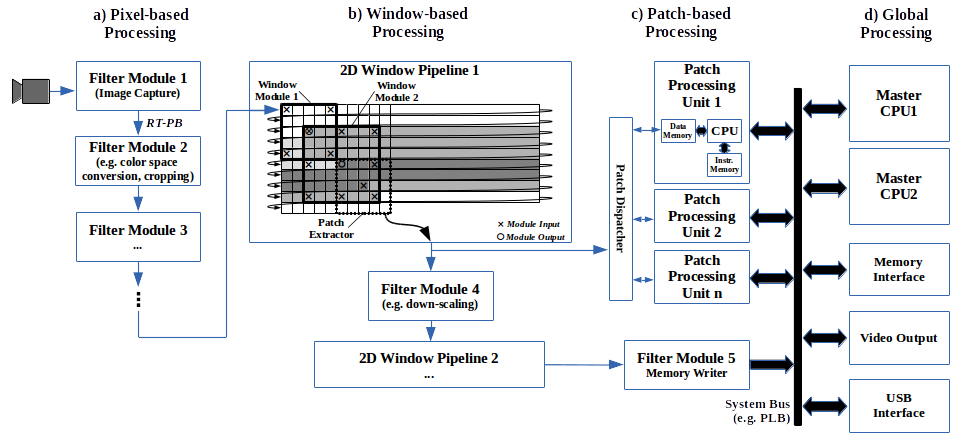
\includegraphics[width=15cm]{figs/01-asterics-example}
        \par\end{centering}
    \caption{Example \asterics system\label{fig:01-asterics-example}}
\end{figure}


\subsection{Interfaces}
\asterics utilizes a modular principle for combining its modules to arbitrary image processing chains.
Great effort has been made to create a set of interfaces for defining the inter-module communication and hardware-software interaction to guarantee a certain behavior within the processing chain and to prevent data loss. 
The interfaces of \asterics are organized as following:

\begin{itemize}
    \item General Interfaces (Chapter~\ref{ch:05-01-interfaces-general})
    \item Common Per-Module Signals (Chapter~\ref{ch:05-02-interfaces-module_signals})
    \item The \asterics Streaming Interface (\texttt{as\_stream}) (Chapter~\ref{ch:05-03-interfaces-as_stream})
    \item The \asterics 2D Window Filter Interface (Chapter~\ref{ch:05-03-interfaces-as_window})
\end{itemize}

\subsubsection{General Interfaces}
This type of interfaces covers general concepts for interaction between hardware and software for a single module as well as a processing chain as whole.
Here, the software is accessing the hardware for obtaining status information and influencing the behavior of the hardware.
This includes the types of errors which may occur within the hardware which have to be addressed by software and the expected behavior of the hardware in case the software \textit{resets} single modules or the processing chain as a whole.
Additional topics are the version management and the i2c bus interface for communicating with external hardware components, which are not part of the programmable logic.

\subsubsection{The Common Per-Module Signals}
These interfaces are used for hardware internal communication to request status information and trigger certain operations, which affect modules as a whole.
These status information include the \texttt{READY} signal, which indicates whether the hardware module is currently operable or the \texttt{SYNC\_ERROR} which signals that data has been lost at some point during operation.
Regarding the operations affecting modules as a whole, signals such as \texttt{RESET} and \texttt{FLUSH} may be present for the module.

The aforementioned interfaces can either be utilized by other \asterics hardware module or by some logic for controlling the entire image processing chain, e.g. to reset all modules at once.  

\subsubsection{The \asterics Streaming Interface (\texttt{as\_stream})}
Signals which are required for controlling the actual data transfers between hardware modules, e.g. the inter-module communication, are summarized here.
The signals \texttt{DATA} and \texttt{STROBE} are used for setting up the most basic data transfers.
The \texttt{as\_stream} interface defines additional signals, mainly for synchronization to provide more detailed information about the data layout, e.g. \texttt{HSYNC} for indicating the start of a new line.
Additionally, the \texttt{STALL} signal is defined by the \texttt{as\_stream} interface for requesting to temporarily suspend data transfers, in case data is processed at a varying pace across hardware modules.


\subsubsection{The \asterics 2D Window Filter Interface}
% TBD: Currently, there are no set rules which define a 2D window filter interface
This type of interface defines a set of signals for hardware modules which operate on a 2D sliding window buffer.


\subsection{Basic Modules}
\asterics offers a wide range of hardware modules for building image processing chains. 
Modules who fulfill a less complex or common task are categorized as basic modules within \asterics. 
The memory modules for transferring data between hardware and software (e.g. \texttt{as\_memreader/-writer}), converters (e.g. \texttt{as\_invert}) or adapters (e.g. \texttt{as\_disperse}, \texttt{as\_mux}) fall into this category.
Although there is no set rule or checklist for defining \textit{basic modules} within \asterics, modules belonging to this category are usually not particularly relevant for the image processing task itself but rather serve a supporting role. 
For this reason, multiple instances of modules of this type can be commonly found across an image processing chain.

The currently available basic modules of \asterics are presented in detail in chapter~\ref{ch:07-modules}.
Some modules may not yet be publicly available due to being currently in development or being in the staging process to be released.
In case you cannot find the documentation for a specific module, please contact one of the authors.
Depending on the stage of the module, its documentation (if already available) or further information regarding the module will be provided.

\subsection{Sophisticated Modules}
Contrary to basic modules, sophisticated modules serve a distinct image processing task which is rather complex and requires a dedicated hardware design in order to be performed efficiently regarding resource consumption and processing speed.
Modules belonging to this category are for example the \textit{Universal Hough Transform} (\texttt{as\_uht}), the \textit{Non-Linear Image Transformation} (\texttt{as\_nitra}) or the \textit{Canny Edge Detector} (\texttt{as\_edge\_and\_scale}).
Due to their unique design and efficient implementation, there is usually also one or more scientific publications associated with the module. 

A detailed description of the sophisticated modules of \asterics are presented in chapter~\ref{ch:08-modules-complex}. 
Some modules may not yet be publicly available due to being currently in development or being in the staging process to be released.
In case you cannot find the documentation for a specific module, please contact on of the authors.
Depending on the stage of the module, its documentation (if already available) or further information regarding the module will be provided.

\subsection{Tools}
A tool is a piece of software, which aids its user at a regularly required or tedious task regarding building or using an image processing chain as a whole or certain aspects of it.
Tools are usually script-based and perform their task in a (semi-)automatic manner.
This includes the \asterics system generator tool \textit{Automatics}.

A detailed documentation of the available tools of \asterics are provided in chapter~\ref{ch:06-tools}.

\subsection{Software Stack and Options}
The software stack is an accumulation of software drivers for the various modules of \asterics, abstraction layers from vendor and platform dependencies and definitions of the actual image processing chain as well as the environment of the software.
The contents of the software stack allows to operate any \asterics-based image processing chain in a convenient manner bare-metal and applications with operating system support.

The contents of the software stack and data transfer schemes are outlined in chapter~\ref{ch:04-software}.

\subsection{Reference and Demo Systems}
The \asterics framework includes at least one reference system and usually some additional demonstration systems featuring specific modules or technologies.
Not all systems described in this document may be available in the repository.
Similarly, not all systems in the repository may be fully documented here.
In case you are interested in a system described here or in an undocumented system, please contact the authors.


%\subsection{Addressing Technology Trends}
%TBD



%\begin{verbatim}
%[[ TBD (AZ/CS/MS/GK) - Zusammenfassung aus FPL2014/EW2015/ASAP2018-Papers ]]
%
%- Typical chain of operations (Bild von FPL mit Puppe)
%- Classification of IP operations (4 classes, Zitat Johnson/Bailey + FPL2014)
%  (Tabelle mit Klassifikation nach FPL-Paper)
%
%- Current trends & how this is addressed in ASTERICS:
%  - complex operations -> 2D Window Filters etc. (-> FPL2014)
%  - SoC chips: Software stack, OS integration
%  - OpenCV integration (in progress)
%  - ROS integration
%\end{verbatim}






\section{Organization of this Document}

This document is divided in two parts. The first part is a user guide and contains all material necessary to understand the basic concepts and to get started using \asterics or eventually developing new \asterics modules or tools.
\begin{itemize}
\item Chapter \ref{ch:01-overview} gives an overview on the \asterics project as a whole.
\item Chapter \ref{ch:02-using} contains all information necessary to start using \asterics and to develop systems containing \asterics chains.
\item Chapter \ref{ch:03-developing} contains all information required to contribute to the \asterics project by developing new modules or tools.
\end{itemize}

The second part serves as a reference guide. 
\begin{itemize}
\item Chapter \ref{ch:04-software} describes the organization of the highly configurable and portable software stack together with all aspects related to the hardware-software interfaces.
\item Chapters \ref{ch:05-interfaces}, \ref{ch:06-tools}, and \ref{ch:07-modules} refer to the three main dimensions of \asterics and give a reference on the interfaces, tools, and commonly used modules, respectively.
\item Chapter \ref{ch:08-modules-complex} gives an overview of the more complex modules of \asterics, such as feature detection or object recognition.
\item Chapter \ref{ch:09-systems} lists a number of "ready-to-use" systems, deploying a specific \asterics chain.
\end{itemize}

In summary, if you are...
\begin{itemize}
\item ... new to \asterics and want to learn about its capabilities and get the demos running on your computer, you should read Chapter \ref{ch:02-using}.
\item ... a new member or partner of the \textit{Efficient Embedded Systems (EES)} group or for some other reason plan to work on the \asterics framework, you should read Chapter \ref{ch:03-developing} to get acquainted with the code organization of the project.
\item ... already an experienced \asterics developer, you will certainly always remember that Chapters \ref{ch:04-software} through \ref{ch:09-systems} serve as a reference manual where you can find any information you may ever need. However, the evolution of this document itself is part of the \asterics development process. If you come across anything missing or outdated, you will also certainly feel the responsibility to add or correct the missing information.
\end{itemize}



\section{Further Reading}

Although the present document covers most information required for utilizing and developing for \asterics, there are also a number of additional resources available.
These resources mainly address more general topics regarding \asterics.


\begin{itemize}
\item The \href{https://ees.hs-augsburg.de/asterics/index_en.html}{\textit{\asterics homepage}} of the \textit{EES} group introduces the framework and lists recent work.
%\item The \href{http://asterics-wiki.informatik.hs-augsburg.de/doku.php}{\asterics wiki} page gives a detailed overview of the framework's structure. 
%The source code can also be obtained from here.
\item The public, open source core of the \asterics framework is available on \href{https://github.com/hsa-ees/asterics}{GitHub} 
\item The source code of \asterics is documented using Doxygen:
\begin{itemize}
\item Hardware module (VHDL) documentation: \refdoxyvhdl
\item Software, driver and support library (C) documentation: \refdoxyc
\item Automatics, the \asterics system generator (Python) documentation: \refdoxypython
\end{itemize}
\item The various concepts and ideas revolving around \asterics are presented in a series of \href{https://ees.hs-augsburg.de/publikationen/index_en.html}{\textit{publications}}.
These comprise, among others, the system generator \textit{Automatics}~\cite{manke_ew2020}, a configurable architecture for the \textit{Generalized Hough Transform}~\cite{kiefer_configurable_2016}, a pipelined architecture for \textit{feature detection}~\cite{pohl_efficient_2014} as well as a module for removing distortion and rectifying images~\cite{pohl_efficient_2012}.
\end{itemize}

%\begin{verbatim}
%- Scientific papers for concepts and ideas: FPL2014, EW2015, ASAP2018, (JImaging 2019)
%- EES Wiki for up-to-date information
%- Doxygen site for code documentation
%- ...?
%\end{verbatim}



\section{Terminology and Conventions}


\subsection{Terminology}

An \textit{ASTERICS~module} is an image processing module, which may be implemented in hardware, in software, or in a combination of both. Modules primarily implemented in hardware (e.~g. filter modules) are referred to as \textit{hardware modules}, those primarily implemented in software (e.~g. \texttt{as\_memio}) are referred to as \textit{software modules}.

An \textit{ASTERICS~chain} is a complete sub-system of connected \asterics modules, typically implementing one or even multiple complete image processing chains. At system level, an \textit{ASTERICS chain} is represented by an IP core on the hardware side and by an \textit{ASTERICS Support Package} in the software side.



\subsection{Conventions}

Throughout this book, the following conventions are used:

\begin{itemize}

\item Signal, variable of function names that can also be found in the code, are written in a \texttt{typewriter font}. Hardware signals are written in \texttt{UPPER\_CASE}, C code functions and module names in \texttt{lower\_case}.

\item \textit{Italic font} is used for emphasis.

\item \textbf{Bold font} is used for definitions.



\end{itemize}

%%%%%%%%%%%%%%%%%%%%%%%%%%%%%%%%%%%%%%%%%%%%%%%%%%%%%%%%%%%%%%%%%%%%%%%%%%%%%%
%%
%% This file is part of the ASTERICS Framework. 
%%
%% Copyright (C) Hochschule Augsburg, University of Applied Sciences
%% Efficient Embedded Systems Group
%%
%% Author(s): Gundolf Kiefer <gundolf.kiefer@hs-augsburg.de>
%%
%%%%%%%%%%%%%%%%%%%%%%%%%%%%%%%%%%%%%%%%%%%%%%%%%%%%%%%%%%%%%%%%%%%%%%%%%%%%%%



%%%%%%%%%%%%%%%%%%% 2. Using ASTERICS %%%%%%%%%%%%%%%%%%%


\chapter{Using \asterics}\label{ch:02-using} 

\secauthor{Michael Schäferling, Gundolf Kiefer, Philip Manke}


\section{Installation}
\label{sec:02-installation}

Prerequisites for the core parts of \asterics:

\begin{itemize}
\item A Linux based operating system. \asterics is tested for Debian 10
\item We strongly recommend the use of the Bourne-Again-Shell \texttt{bash} for \asterics scripts and Makefiles
\item GNU \texttt{make}
\item Python3, version \texttt{3.5} or higher
\item Python packages: \texttt{numpy} (for generating CNN systems)
\end{itemize}

\asterics-GUI prerequisites:

\begin{itemize}
\item Python packages: \texttt{pyqt5}, \texttt{pandas}.
\item QT5, version \texttt{5.5} or higher
\end{itemize}

Optional prerequisites:

\begin{itemize}
\item Xilinx Vivado 2019.1 (IP-Core packaging and/or synthesizing systems)
\item GraphViz, version \texttt{2.38} or higher (SVG graph generation)
\item Python package \texttt{graphviz}, version \texttt{0.8} or higher (SVG graph generation)
\end{itemize}


The \asterics framework can be used in two ways:

\begin{itemize}
\item As a \textit{portable} installation or
\item as a \textit{fixed} system installation.
\end{itemize}

The \textit{portable} installation is essentially a clone of the \asterics Git repository (Chapter \ref{ch:03-developing}) or an extracted a repository snapshot.
To utilize \asterics in this form, \textit{source} the file \texttt{settings.sh} in the repository's root folder, using:

\begin{lstlisting}[style=shell]
  $ source settings.sh
\end{lstlisting}

\bigskip

The \textit{fixed} installation requires a clone or extracted snapshot of the \asterics Git repository.
To install \asterics to your system, use the provided makefile install target:

\begin{lstlisting}[style=shell]
  $ make install PREFIX=<install path>
\end{lstlisting}

You may need to provide root permissions depending on your installation path.
To now use the installation, you need to source the file \texttt{settings.sh}, as you would for the portable installation.

\begin{lstlisting}[style=shell]
  $ source <install path>/settings.sh
\end{lstlisting}

Optionally, for convenience, we suggest adding an alias for the sourcing command to your \texttt{.bashrc} file.


\section{Getting Started with the Supplied Demo System}
\label{sec:02-getting_started}

The \asterics framework provides at least one demonstration system to get in touch with the concepts of the framework and its modules.
The system may also be used as a basis for further development.

The demo system is equipped with a \texttt{Make} based build system.
With this, a specific \asterics chain is prepared, which is then integrated into the system during the build step.
During the build step, the required embedded software for proper operation is also supplied.
After hardware synthesis and software compilation, the demo system can be put into operation on the specific board.
The system is tested using Vivado versions 2019.1 and 2020.2.


In section \ref{sec:06-02-user_guide} a short user guide describes the necessary steps for building the demo system \texttt{as\_refdesign\_zynq} with a focus on the \asterics system generator \textit{Automatics}.
Here, \textit{Automatics} is described in less detail with more focus on the build process itself.

The following prerequisites are necessary to build and use the demo system:

\begin{itemize}
\item (optional) A hardware target. To run the demo system as is, the Zybo\footnote{\url{https://store.digilentinc.com/zybo-zynq-7000-arm-fpga-soc-trainer-board/}} board and an OmniVision OV7670 camera module are required. Necessary cable drivers and board files need to be installed.
For other hardware targets, the constraint files and the Vivado project (block design) need to be modified manually.
\item (optional) To view the demo system in action, a monitor with a VGA or HDMI input connected to the hardware is required.

\bigskip
\emph{NOTE:} If your Linux distribution does not support the \texttt{source} command by default (Ubuntu, Debian, ...), it does not use \textit{bash} as the standard shell. You need to either modify this setting system-wide or explicitly run each of the files that is passed to the \texttt{source} command in the steps below.


\end{itemize}

Follow the following steps to build the demo system \texttt{"as\_refdesign\_zynq/"}:

\begin{enumerate}

\item Setup and optionally install \asterics. Refer to Section \ref{sec:02-installation} for this step.
\item Source your \asterics installation:
	\begin{lstlisting}[style=Shell]
 > source <asterics root / installation>/settings.sh
  \end{lstlisting}
\item Set up a workspace directory and move into it:
  \begin{lstlisting}[style=Shell]
 > mkdir asterics-workspace && cd asterics-workspace
  \end{lstlisting}
\item Copy the directory \texttt{asterics/systems/as\_refdesign\_zynq/} to your workspace:
  \begin{lstlisting}[style=Shell]
 > cp -a <asterics root / installation>/systems/as_refdesign_zynq/ .
  \end{lstlisting}
\item Optional: If you intent to build the Vivado IP-Core (also needed to build the whole system), you need to source your Vivado installation:
  \begin{lstlisting}[style=Shell]
 > source <VIVADO-DIR>/settings64.sh
  \end{lstlisting}
\item Move into \texttt{as\_refdesign\_zynq/} in your workspace:
  \begin{lstlisting}[style=Shell]
 > cd as_refdesign_zynq
  \end{lstlisting}
\item Now you can build the system. You can generate only the \asterics source files using:
  \begin{lstlisting}[style=Shell]
 > make asterics_core
  \end{lstlisting}
  \textbf{This generates the \asterics hardware (VHDL) and software (C) files for the demo system to \texttt{./asterics\_core}.
  From here you can inspect the files, modify them and/or include them in your projects or FPGA toolchains other than Xilinx Vivado.}

\item If Vivado is available, you can generate Xilinx-specific output products:
	{
    \begin{enumerate}
	\item You can generate the \asterics IP-Core (to be used in a Vivado project) using:
    \begin{lstlisting}[style=Shell]
 > make asterics_vivado_cores
    \end{lstlisting}
    The IP-Core will be generated to the directory \texttt{vivado\_cores}.
    From here you can include this directory into the IP-Catalogue of Vivado.
    Now you can inspect the IP-Core and add it to block designs.
  \item You can build the entire FPGA project (after the Vivado IP-Core was generated, see above), using:
    \begin{lstlisting}[style=Shell]
 > make build_system
    \end{lstlisting}
  Note that this will take some time, depending on the capabilities of your development system.
  This creates and builds a full Vivado project with a block design targeting the ZYBO board.
  After synthesis and implementation you can open the project in the GUI using:
  \begin{lstlisting}[style=Shell]
 > vivado hardware/build/system.xpr
  \end{lstlisting}
  \item If you have a ZYBO board and OV7670 image sensor board handy, you can program the hardware and software onto the target boards FPGA by running:
    \begin{lstlisting}[style=Shell]
 > make run
    \end{lstlisting}
  \item Alternatively: To build, implement and compile the hardware and software and flash it onto the board in one step, you can execute:
    \begin{lstlisting}[style=Shell]
 > make build_and_run
    \end{lstlisting}
  or
    \begin{lstlisting}[style=Shell]
 > make all
    \end{lstlisting}
	\end{enumerate}
	}
\end{enumerate}


\section{Getting Started with the \asterics GUI}

\infobox{The \asterics-GUI is still in development and not fully tested. See the application and this documentation as in-flux and experimental.}

The \asterics framework provides a Graphical User Interface (GUI), which is currently under development, with some basic features already available.
Currently, the GUI provides a module browser with information about all modules that come with \asterics and a wizard for setting up Automatics scripts for demo systems and simple systems from scratch.

For more information on the \asterics-GUI and for a user guide, see Section \ref{ch:06-05-tools-gui}.


\section{How to Design \asterics Systems}
\secauthor{Philip Manke}

The \asterics system generator tool \textit{Automatics} automates most of the process of generating an \asterics system and packaging it into an IP-Core and is the official way to create \asterics systems.

\subsection{Design Flow Overview and Terminology}

To start working with \asterics, first an \asterics installation must be procured.
For instructions refer to section \ref{sec:02-installation}.


Generally, we recommend using a Linux based operating system for working with \asterics, as most tools are used on the command line and Makefiles are supplied to automate portions of the process of building \asterics systems.
Furthermore, MAC OS and Microsoft Windows have not been tested.

\subsubsection*{Terminology}

\begin{itemize}
\item \textbf{\asterics:} The entire framework. This includes everything within the git repository.
\item \textbf{\asterics Installation:} A local copy of the \asterics git repository at a known location.
\item \textbf{\asterics Settings File:} A short script that is used to set certain environment variables required by some tools to function correctly and be available from the command line. Used best with the \texttt{source} command.
\item \textbf{IP-Core:} An Intellectual Property - Core (IP-Core) is a packaged hardware and software subsystem for integration into a larger system.
\item \textbf{Hardware Module:} A module with purely hardware source files. 
\item \textbf{Software Module:} A module with purely software source files.
\item \textbf{\asterics Module:} A hardware and / or software module included with \asterics. These modules are manually developed and provide common functionality. They may describe image processing operations, common data management tasks, infrastructure or support other modules similar to a library. They are contained in the \texttt{modules} folder.
\item \textbf{Module Repository:} A directory containing \asterics modules using the file structure laid out in section \ref{sec:02-file_structure}.
\item \textbf{\asterics Chain / \asterics System / \asterics IP-Core:} A specific configuration built from \asterics modules, comprising both hardware and software.
It must be integrated into a larger system to be synthesized and programmed onto an actual hardware target.
These terms are often used interchangeably, though generally \asterics chain specifically refers to the concept of the \asterics subsystem of modules, \asterics system may also refer to a larger system that has an \asterics chain integrated into it and \asterics IP-Core may refer specifically to an \asterics chain that was packaged to an IP-Core to be integrated into a larger system.
\item \textbf{Generic:} A configuration parameter for an \asterics module. This name comes from the hardware description language VHDL, that all modules are written in.
\item \textbf{Port:} A single input or output for data or control signals of a hardware module.
\item \textbf{Interface:} A standardized arrangement of ports. The name, data type, direction and function of each port is defined.
\item \textbf{Automatics:} The \asterics system generator tool.
\item \textbf{Chain Description Script:} Build instructions for Automatics in Python syntax to build an \asterics chain.
\item \textbf{Module Specification Script:} A small Python script providing meta-information for each \asterics module.
Automatics requires this script to analyse an \asterics module - one script per module.
\item \textbf{2D Window Pipeline:} A hardware architecture for the efficient implementation of sliding window buffers, required by systems with multiple window modules.
\item \textbf{Window Module / Filter Module}: An \asterics module for use within a 2D Window Pipeline.
This kind of module has a special input port to receive multiple pixels from different locations in the image simultaneously.
\end{itemize}

\subsubsection*{\asterics Design Flow}
The following list describes the broad steps of the typical design flow for \asterics systems:

\begin{enumerate}
\item The process of using \asterics always begins with sourcing the \asterics settings file, as described in section \ref{sec:02-getting_started}.
\item We recommend to start the command line interface (CLI) or the graphical version (GUI) of the \asterics module browser to get an overview of available \asterics module, their interfaces, ports and configuration generics.
Using the tools, \asterics modules for use in the processing chain and functionalities that may require new modules are identified.
\item To get started quickly, we recommend to copy an existing system from \texttt{asterics/systems/}.
At least a new (blank) chain description script for the \asterics chain and any hardware specific files, such as constraint files, are required.
\item To describe your system using Automatics, the chain description script must be edited.
In the example system it can be found in \lsthdlinline{as\_refdesign\_zybo/asterics/image\_differencing/asterics-gen.py}
\item Using a module browser (GUI or CLI) to identify the names of the desired modules they are added to the chain description, configured and connected with each other.
\item If hardware modules not provided by \asterics are to be used:
	\begin{enumerate}
	\item The module source files are organized in a separate module repository, according to the file structure laid out in section \ref{sec:02-file_structure}.
	\item A module specification script is created for the module detailed in section \ref{sec:06-02-new_modules}.
	\item The module browser is used to analyze the modules by adding the module repository.
	The modules are inspected to make sure they were analyzed correctly.
	\item The module repository import is added to the chain description script.
	\end{enumerate}
\item Desired output products are added to the chain description script and Automatics is run.
\item The generated hardware files may be inspected for any errors.
\item If the Xilinx toolchain is used, Automatics can automatically package the \asterics chain as a Vivado-compatible IP-Core, otherwise the resulting hardware and software files have to be packaged manually.
\item The \asterics IP-Core is integrated into the larger system. \asterics provides AXI slave and master ports for communication.
\end{enumerate}

These major steps are described in detail in the following subsections.


\subsection{Settings up a new Project with Automatics}
\label{ssec:02-setup}

This section details the typical steps necessary to set up a new project using Automatics.


\subsubsection{Setup Steps:}

\begin{enumerate}
\item Install \asterics. See Section \ref{sec:02-installation}.
\item Open a command line interface (preferably using \texttt{bash})
\item Source the \asterics settings file in the installation directory using:
\begin{lstlisting}[style=Shell]
 > source <path to installation>/settings.sh
\end{lstlisting}
\item Create a new project directory and change into it:
\begin{lstlisting}[style=Shell]
 > mkdir <new project system name>
 > cd <new project system name>
\end{lstlisting}
\item Create a new chain description script:
\begin{lstlisting}[style=Shell]
 > touch asterics-gen.py
\end{lstlisting}
\item Open the chain description script in your editor of choice.
We recommend a Python-capable IDE, with the Automatics source files added to the list of auto-complete sources for the best experience.
\end{enumerate}

The entire \asterics chain will now be described in the chain description script using Python commands.
Using Automatics with this description, all necessary hardware files implementing the described chain will be generated and all module source files necessary to implement and use the chain will be collected.

To get started with the chain description script, the following two lines need to be added:
\begin{lstlisting}[style=AutomaticsPython]
 import asterics
 chain = asterics.new_chain()
\end{lstlisting}

The first line imports the \lstapyinline{asterics} Python module.
This makes the highest level functions of Automatics available in the rest of the file.
The second line makes use of the \lstapyinline{asterics} Python module, creating a new \lstapyinline{chain}.
Writing \lstapyinline{chain} to the left of the equals sign, assigns the newly created chain to the keyword (variable) \lstapyinline{chain}.
Using \lstapyinline{chain}, the rest of the \asterics chain can now be described.

\subsubsection{Configuring Automatics for the Hardware Target}
\label{ssec:02-hwtargetconfig}

By default Automatics is configured to generate IP-Cores compatible with ZYNQ-7000 series FPGA-SoCs by Xilinx, specifically, the ZYBO development board by Digilent Inc is used as the reference board.

Certain parameters have to be explicitly provided in the chain description script to target a different FPGA.

The following commands are provided by Automatics:\\
\begin{itemize}
\item \lstapyinline{chain.define_hardware_target("partname", "design name", "board")}\\
This command defines which FPGA part the generated IP-Core is compatible with (\texttt{"partname"}), the internal name of the packaged IP-Core (\texttt{"design name"}) and the specific FPGA board it is packaged for (\texttt{"board"}).
These parameters only apply to automatic IP-Core packaging using Automatics and Xilinx Vivado.
\item \lstapyinline{chain.set_ipcore_name("name", "description")}\\
This command sets display name of the packaged IP-Core (\texttt{"name"}) and its description (\texttt{"description"}).
These values will be visible in the IP Repository of Xilinx Vivado.
These parameters only apply to automatic IP-Core packaging using Automatics and Xilinx Vivado.
\item \lstapyinline{chain.set_asterics_base_address(<address>, <address space size>)}\\
This command changes the base address and optionally the size of the address space for the \asterics IP-Core.
The base address is required as the slave register manager of \asterics requires to know the base address in order to decode them.
The address space size has no impact on the hardware generated.
Automatics uses it to warn the user if too many registers are present in an \asterics chain, not mappable to the register address space.
\end{itemize}

\subsection{Adding Modules to the \asterics Chain}
\label{ssec:02-adding}

An \asterics chain consists of \asterics modules that each fulfill cohesive tasks to comprise a complete image, video or general data processing system.
Modules may have tasks such as data management, general infrastructure, image processing, general processing, etc.

The \asterics installation provides a collection of modules, free to use.
To browse the available modules in a graphical user interface using QT5, use:
\begin{lstlisting}[style=Shell]
 > as-module-browser
\end{lstlisting} 

Alternatively, a command line interface is available with:
\begin{lstlisting}[style=Shell]
 > as-module-browser-cli
\end{lstlisting}

Once a desired module is determined, it can be added to the \asterics chain using the following command:
\begin{lstlisting}[style=AutomaticsPython]
module = chain.add_module("entity name")
\end{lstlisting} 

To tell Automatics which module should be added to the chain, provide the entity name of the module to the command \lstapyinline{add_module}.
Both the CLI and GUI module browser list this name for each module.
As with the chain object, the newly added module is also assigned to a new keyword, so it can be referenced later in the chain description script.
Use a short but memorable and easily identifiable name for each module you add to the chain, for example:
\begin{lstlisting}[style=AutomaticsPython]
result_writer = chain.add_module("as_memory_writer")
\end{lstlisting}

Additionally, two further parameters can be provided to the command \lstapyinline{add_module}:

The second parameter, \texttt{user name}, will optionally name the hardware module instantiated in the generated files.
Signals that connect from the module will also be generated with the provided name included, making the generated code easier to read and especially making it easier to distinguish external interfaces of the resulting IP-Core.

The third parameter, \texttt{repo\_name}, optionally defines from which module repository the requested module should be selected.
It is only necessary to define the repository, if two modules with the same \texttt{entity name} exist, for example, if a modified version of a standard \asterics module exists.

The \lstapyinline{add_module} command with all three parameters may look like this:
\begin{lstlisting}[style=AutomaticsPython]
camera = chain.add_module("as_sensor_ov7670", "cam0", "default")
\end{lstlisting}

If custom modules are to be used with Automatics, they first have to be imported.
To import new modules to Automatics, the following command is used in the chain description script:
\begin{lstlisting}[style=AutomaticsPython]
asterics.add_module_repository("path", "repository name")
\end{lstlisting}
The parameter \texttt{"path"} of the command tells Automatics, where to look for new modules.
The path to a directory that is organized in the same way as the \texttt{modules} directory of \asterics, as described in section \ref{sec:02-file_structure}, should be provided.
The parameter \texttt{"repository name"} is optional and can be set to any name desired.
It may prove useful to differentiate between multiple imported module repositories, as specific repository can be defined when using the \lstapyinline{add_module()} command is used.
The command can be used at any point after \lstapyinline{import asterics} in the chain description script, however, we recommend putting it before the command creating a new chain.

\subsection{Configuring \asterics Modules}
\label{ssec:02-configuring}

This section gives a basic overview of the most common configuration options for \asterics modules.
Section \ref{ssec:02-example-script} provides a short example script with valid configuration commands.

\subsubsection{Configuring Module Parameters: Generics}

Modules added to the chain can be configured with their own parameters, using \textit{Generics}.
Each module has a different set of generics, most with default values, if they are not explicitly assigned a value in the chain description script.

The generics and their default values of a module are available using a module browser or by directly consulting the source code of the module.
The effect of each generic is currently only explained either in the source code of the module of in the reference of the module in this manual.

Assigning a new value to the generic is done using the following command:
\begin{lstlisting}[style=AutomaticsPython]
module.set_generic_value("GENERIC NAME", "value")
\end{lstlisting}

To tell Automatics which generic to modify, the \texttt{GENERIC NAME} specifies the generic using its name as it appears in the source code.
The module browsers list the generic's names for all modules.

The \texttt{value} is what the generic will be assigned.
This parameter can be any number (integer or float) or string.

\emph{Note:}
The value provided for the \texttt{value} parameter will be directly written into the generated source code.
For example: To set the generic \texttt{KERNEL\_TYPE} of the module \texttt{conv\_filter} to \lsthdlinline{"laplace"}, the following command has to be used:
\begin{lstlisting}[style=AutomaticsPython]
conv_filter.set_generic_value("KERNEL_TYPE", '"laplace"')
\end{lstlisting}

Note how the double quotes of the value \lsthdlinline{"laplace"} are only carried over to generated VHDL code if they are inside a string themself, by using single quotes to encompass the entire value.
The same can be achieved using triple double quotes: \lstapyinline{""" "laplace" """} or by escaping the double quotes: \lstapyinline{"\\"laplace\\""}.
Similarly, for \lsthdlinline{std_logic} values, delimited in VHDL by single quotes, these have to be encased in double quotes in the chain description script, for example:
\begin{lstlisting}[style=AutomaticsPython]
module.set_generic_value("EXAMPLE_GENERIC", "'0'")
\end{lstlisting}

\subsubsection{Configuring Module Ports}

For some ports of modules you may want to assign a static value, for example if the functionality of the port is not used in the specific chain that is described.
By default Automatics will assign a \textit{neutral value} to ports that are left unconnected.
This value depends on the data type and direction of the port, for further details, refer to section \ref{sec:06-02-default}.
To assign a static value to a port, use the following command:
\begin{lstlisting}[style=AutomaticsPython]
module.set_port_fixed_value("port name", value)
\end{lstlisting}
To tell Automatics which port should be modified, the name of the port must be provided as the first parameter to this command.
To assure that the correct port is selected, the full name of the port should ideally be provided.
As with assigning values to generics, the value of the parameter \texttt{value} will be directly inserted into the generated VHDL code and must therefore follow VHDL syntax.
The following are examples for the correct use of the command:
\begin{lstlisting}[style=AutomaticsPython]
result_writer.set_port_fixed_value("mem_req_ack", "'1'")
image_reader.set_port_fixed_value("stall_out", "open")
edge_filter.set_port_fixed_value("threshold", 'X"C418"')
inverter.set_port_fixed_value("data_in", "s_camera_data(7 downto 0)")
\end{lstlisting}

Furthermore, ports may also be configured to face the outside of the entire \asterics chain.
For example, if an external device, such as a video camera, is to be connected to the \asterics chain, the module that should be connected to the device needs to provide the necessary ports for it.
These ports must be available as ports of the \asterics IP-Core, at the highest level of the chain, or \textit{external}.
For this and similar purposes, ports can be \textit{made external} using the following command:
\begin{lstlisting}[style=AutomaticsPython]
module.make_port_external("port name", value)
\end{lstlisting}
To tell Automatics which port of the module to modify, the port's name must be provided as the first parameter for this command.
The second parameter is optional and by default is taken to be set to \lstapyinline{True}.
If set to \lstapyinline{True}, the command will make the port external.
If set to \lstapyinline{False}, the command can make reverse the effect of making a port external.
Some ports are set to be external by default, this command can make these ports "internal" again.
The following are examples for the correct use of the command:
\begin{lstlisting}[style=AutomaticsPython]
result_writer.make_port_external("flush")
camera.make_port_external("data_in", True)
image_reader.make_port_external("flush_in", False)
\end{lstlisting}

\subsubsection{Configuring Module Interfaces}

An interface of an \asterics module is a collection of ports.
As with ports, an entire interface may also be configured to face the outside of the \asterics chain to be connected with other IP-Cores or external devices later.
For this a similar command is available:
\begin{lstlisting}[style=AutomaticsPython]
module.make_interface_external("interface name", "direction",
                               "interface type", value)
\end{lstlisting}
To tell Automatics which interface to modify, the first three parameters are used to provide identifying information about the interface.
The interface's name suffices in many cases, which is why the other parameters are optional.
If the name is ambiguous, the interface's direction and type should be provided to uniquely identify the desired interface.
The parameter \texttt{value} can be used to invert the functionality of this command, making already external interfaces internal, by setting the parameter to \lstapyinline{False}.

\subsection{Describing Connections}
\label{ssec:02-connecting}

\asterics chains process data that flows through the system in a way akin to a pipeline.
Data is passed from module to module, being processed each step of the way.
In Automatics, the connections are handled in a per-port manner, each port is connected individually.
However, not every connection of every port has to be explicitly described.
Section \ref{ssec:02-example-script} provides a short example script with valid connection commands.

\subsubsection{Connection Commands}

Automatics provides the following ways to connect ports, entire interfaces and entire modules with each other:\\
\begin{itemize}
\item \lstapyinline{module0.connect(module1)}\\
The most general way to describe a connection.
For all unconnected source ports and source interfaces of \lstapyinline{module0} a connection with any matching sink port and sink interface of \lstapyinline{module1} is attempted.
Automatics has several built-in checks to prevent connections between incompatible ports.
For example, the port direction and the data type are checked before a connection is committed.
Similarly, for interfaces, their direction and interface types are also checked to match.
Modules must always be connected in the direction of data flow:
The data source module must be to the left of the \lstapyinline{connect()} command, the data sink module within the parenthesis of the \lstapyinline{connect()} command.
\item \lstapyinline{module0.get_interface("interface name").connect(module1)}\\
To more precisely describe a connection of an interface, the command \lstapyinline{module.get_interface("interface name", "direction", "interface type")} can be used.
The second and third parameters are optional and only required if the interface name alone would be ambiguous.
Use a module browser to find interface names, directions and types of modules.
The \lstapyinline{get_interface()} command followed by \lstapyinline{connect()} tells Automatics to apply the connection only to the interface specified.
If an entire module is provided for the connection target, Automatics will connect the interface to the first matching interface that is found in the module.
\item \lstapyinline{module0.get_port("port name").connect(module1)}\\
To define a single port that should be connected, the \lstapyinline{get_port("port name")} command can be used.
Use a module browser to find the port names of modules.
This command followed by the \lstapyinline{connect()} command tells Automatics to apply the connection only to the port specified.
If an entire module is specified, Automatics will connect the port to the first matching port of the target module.
\item \lstapyinline{module0.get_interface("interface name").connect(module1.get_interface("interface name"))}\\
For precise interface to interface connections, an interface can be provided to the \lstapyinline{connect()} as well.
In this case, Automatics will only attempt a connection between the specified interface of \lstapyinline{module0} and the specified interface of \lstapyinline{module1}.
For example, the following command will connect the output interface of \lstapyinline{camera} with the input of \lstapyinline{writer}:\\
\lstapyinline{camera.get_interface("out").connect(writer.get_interface("in"))}
\item \lstapyinline{module0.get_port("port name").connect(module1.get_interface("interface name"))}\\
This command causes Automatics to attempt connections between the port specified of \lstapyinline{module0} and the ports of the interface specified of \lstapyinline{module1}.
The port will be connected to the first matching port of the interface.
\item \lstapyinline{module0.get_port("port name").connect(module1.get_port("port name"))}\\
This command is the most precise connection command, specifying only a source and target port, therefore only a single connection is attempted.
This command is special, as an important check of the connection process is skipped.
Specifically, the check for equality of the ports' names, allowing the connection between two ports with different names. 
\end{itemize}

\subsubsection{Recommendations and General Rules}

The following list contains general rules and recommendations that apply to the \lstapyinline{connect()} command:

\begin{itemize}
\item Connections to multiple targets, from a port or interface with the direction \lstapyinline{"out"} to ports or interfaces with the direction \lstapyinline{"in"}, are possible by simply using the two necessary connect commands.
Connections from multiple sources to the same target are not allowed as they would in most cases result in problems when synthesizing the resulting hardware description.
\item The \lstapyinline{connect()} command is mostly direction agnostic.
Except when specifying an entire module, the interfaces and ports provided will be internally sorted into source and sink.
However, to be more consistent and readable in the chain description script, we strongly recommend to always write the data source, direction \texttt{out}, to the left of the \lstapyinline{connect()} command and the data sink, direction \texttt{in}, within the parentheses of the \lstapyinline{connect()} command.
\item We recommend to use the commands \lstapyinline{get_interface()} and \lstapyinline{get_port()} especially for modules with many ports and or interfaces.
For simple modules the short-hand command \lstapyinline{get()} generally suffices.
\lstapyinline{get("name", "direction", "interface type")} is a combination of the interface and port specification commands, first searching for an interface of the provided name and then for ports.
As it is possible that a port and interface have the same name, using this method is only recommended when used with simple modules or by more experienced users of Automatics.
\end{itemize}

\subsubsection{Example Chain Description Script}
\label{ssec:02-example-script}

For complete example chain description scripts, refer to section \ref{sec:06-02-user_guide} and the reference designs provided with \asterics in \texttt{asterics/systems/}.

The following are examples for the correct usage of the \lstapyinline{connect()} command in the context of an example chain description script:
\begin{lstlisting}[style=AutomaticsPython]
# Setup:
import asterics
chain = asterics.new_chain()

# Add modules to the chain:
camera = chain.add_module("as_sensor_ov7670")
collect = chain.add_module("as_collect")
writer = chain.add_module("as_memwriter")

# Configuration examples using the writer module:
# Define generic values
writer.set_generic_value("DIN_WIDTH", 32)
writer.set_generic_value("MEMORY_DATA_WIDTH", 32)
# Configure "flush_in" port: 
# Make it available in the interface of the IP-Core
writer.make_port_external("flush_in")

# Connection examples
# Connecting camera and collect (interfaces of type "as_stream"):
camera.connect(collect)
# or
camera.get_interface("out").connect(collect)
# or
camera.get("out", "out", "as_stream").connect(
    collect.get("in", "in", "as_stream")
)
# or
camera.get_port("data_out").connect(collect.get_port("data_in"))
camera.get_port("strobe_out").connect(collect.get_port("strobe_in"))
# ...
camera.get_port("vsync_out").connect(collect.get_port("vsync_in"))

# Connecting collect with writer
# Valid
collect.connect(writer)
# Incorrect, not consistent with the direction of data flow
writer.connect(collect)
# Valid, data flow restriction only applies to modules,
#    not interfaces and ports
writer.get_interface("in").connect(collect.get_interface("out"))
\end{lstlisting}


\subsection{2D Window Pipeline Subsystems}
\label{ssec:02-2dwpl}

This section first provides a brief explanation of the concept of 2D Window Pipeline architectures,  followed by the steps required to describe a 2D Window pipeline implementation using Automatics.
The makeup of window modules and difference to regular \asterics modules will also be touched upon.

\subsubsection{What is a 2D Window Pipeline?}

In a nutshell: The 2D Window Pipeline is a hardware architecture for the efficient implementation multiple sliding window buffers.

\subsubsection{Sliding Window Buffers}

A sliding window buffer is required for processing modules that need access to multiple pixels of the input image at once.
This includes modules that implement image convolution with a kernel, such as Gauss, Sobel and Laplace filters, as well as morphological operations, such as opening and closing and comparison operations such as non-maximum-suppression.

\begin{figure}[htb]
\centering
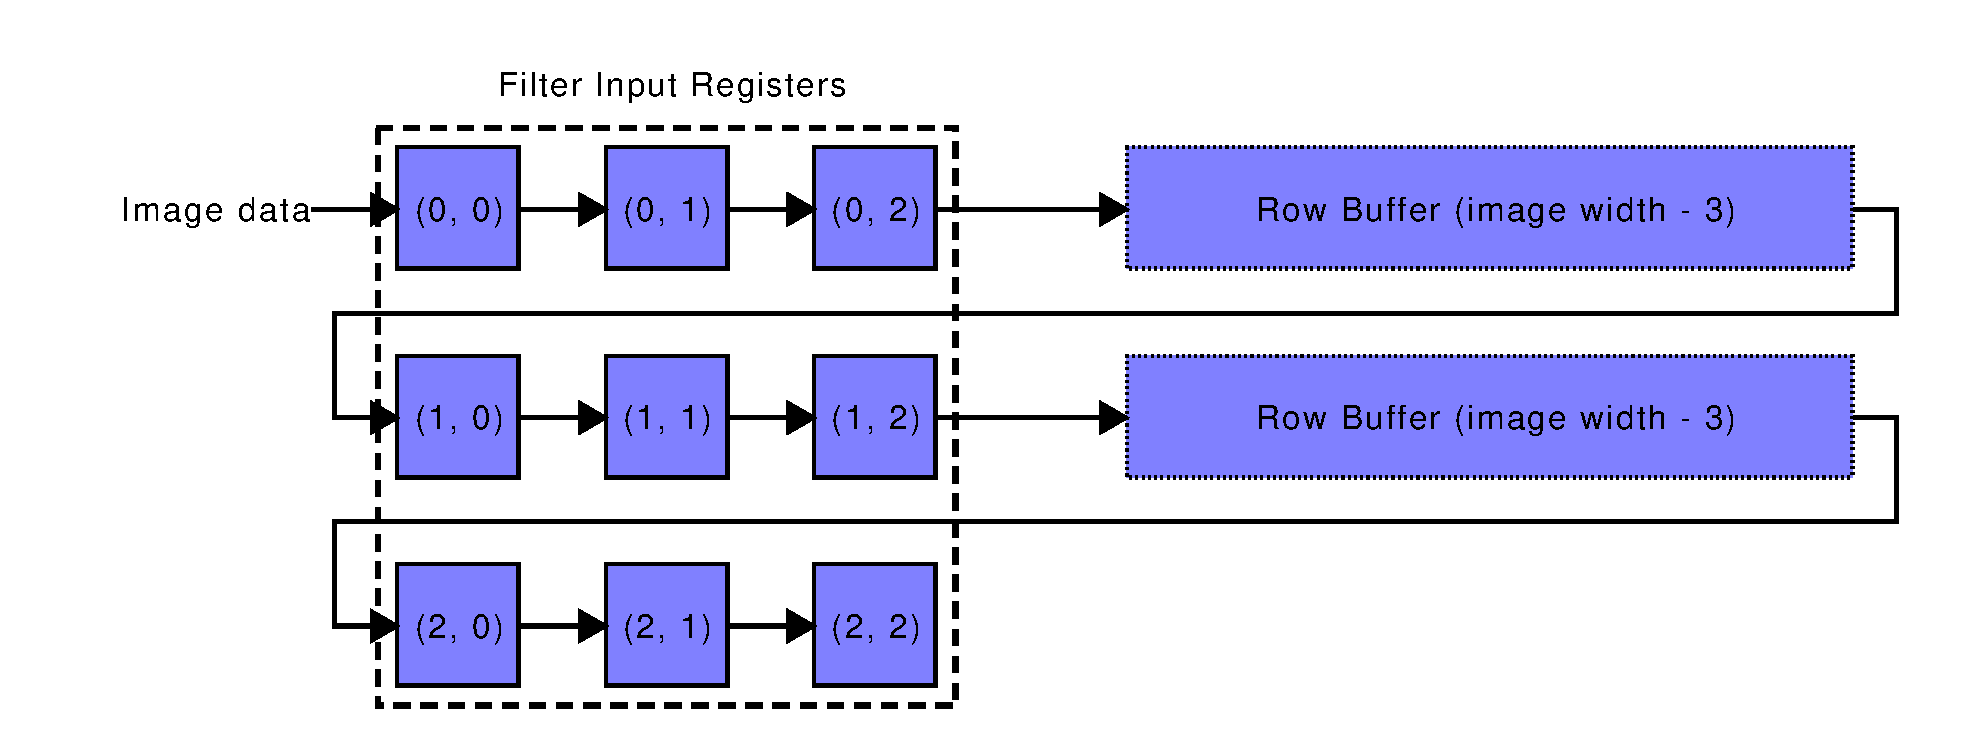
\includegraphics[width=\textwidth]{figs/02-window_buffers_visual.pdf}
\caption{Representation of a sliding window buffer with window size 3 by 3.}
\label{fig:02-sliding_window_buffer}
\end{figure}

Figure \ref{fig:02-sliding_window_buffer} shows a representation of a sliding window buffer as it may be implemented in hardware.
The small cubes represent the hardware registers required to store a single pixel of the image.
Each register contains the relative pixel coordinates.
As the image processing module must have direct and simultaneous access to all pixels in the \textbf{Filter Window}, registers \textit{have} to be used to store those pixels.
The \textbf{Row Buffer}s each store the remaining pixels of a single image row.
For the window size of 3 by 3, as shown in the figure, two complete rows of the image, plus three pixels have to be stored in hardware to implement immediate access to all pixels used by the filter.
This \textbf{sliding window buffer} effectively implements a hardware component that provides a small section of the image to the processing module, the filter window.
By feeding a pixel stream into the buffer, the section moves across the image one pixel at a time for every pixel inserted into the buffer.
The row buffers effectively delay the pixels that are input to them, so they line up with the other pixels within the filter window.
This means that, per pixel input to the sliding window buffer, only one pixel is read from the row buffer  and only one pixel is written to the buffer.
Thus, more efficient memory components, such as block RAM, can be used to implement the buffers.

\subsubsection{2D Window Pipelines}

Oftentimes, image processing systems require multiple filter operations that each require access of multiple pixels simultaneously, for example the Canny edge detector.
In the case of a simple implementation of a Canny edge detector, five processing modules require filter windows of various sizes.
Most modules require a window of the image after it was processed by a previous filter module in the image processing chain.
For these kind of systems, the 2D Window Pipeline architecture can optimize the row buffers required for all of the sliding window buffers.
By merging the row buffers and using block RAM memory components to store large amounts of pixel data, the 2D Window Pipeline can substantially reduce the amount of hardware resources required by the sliding window buffers.

\begin{figure}[htbp]
\centering
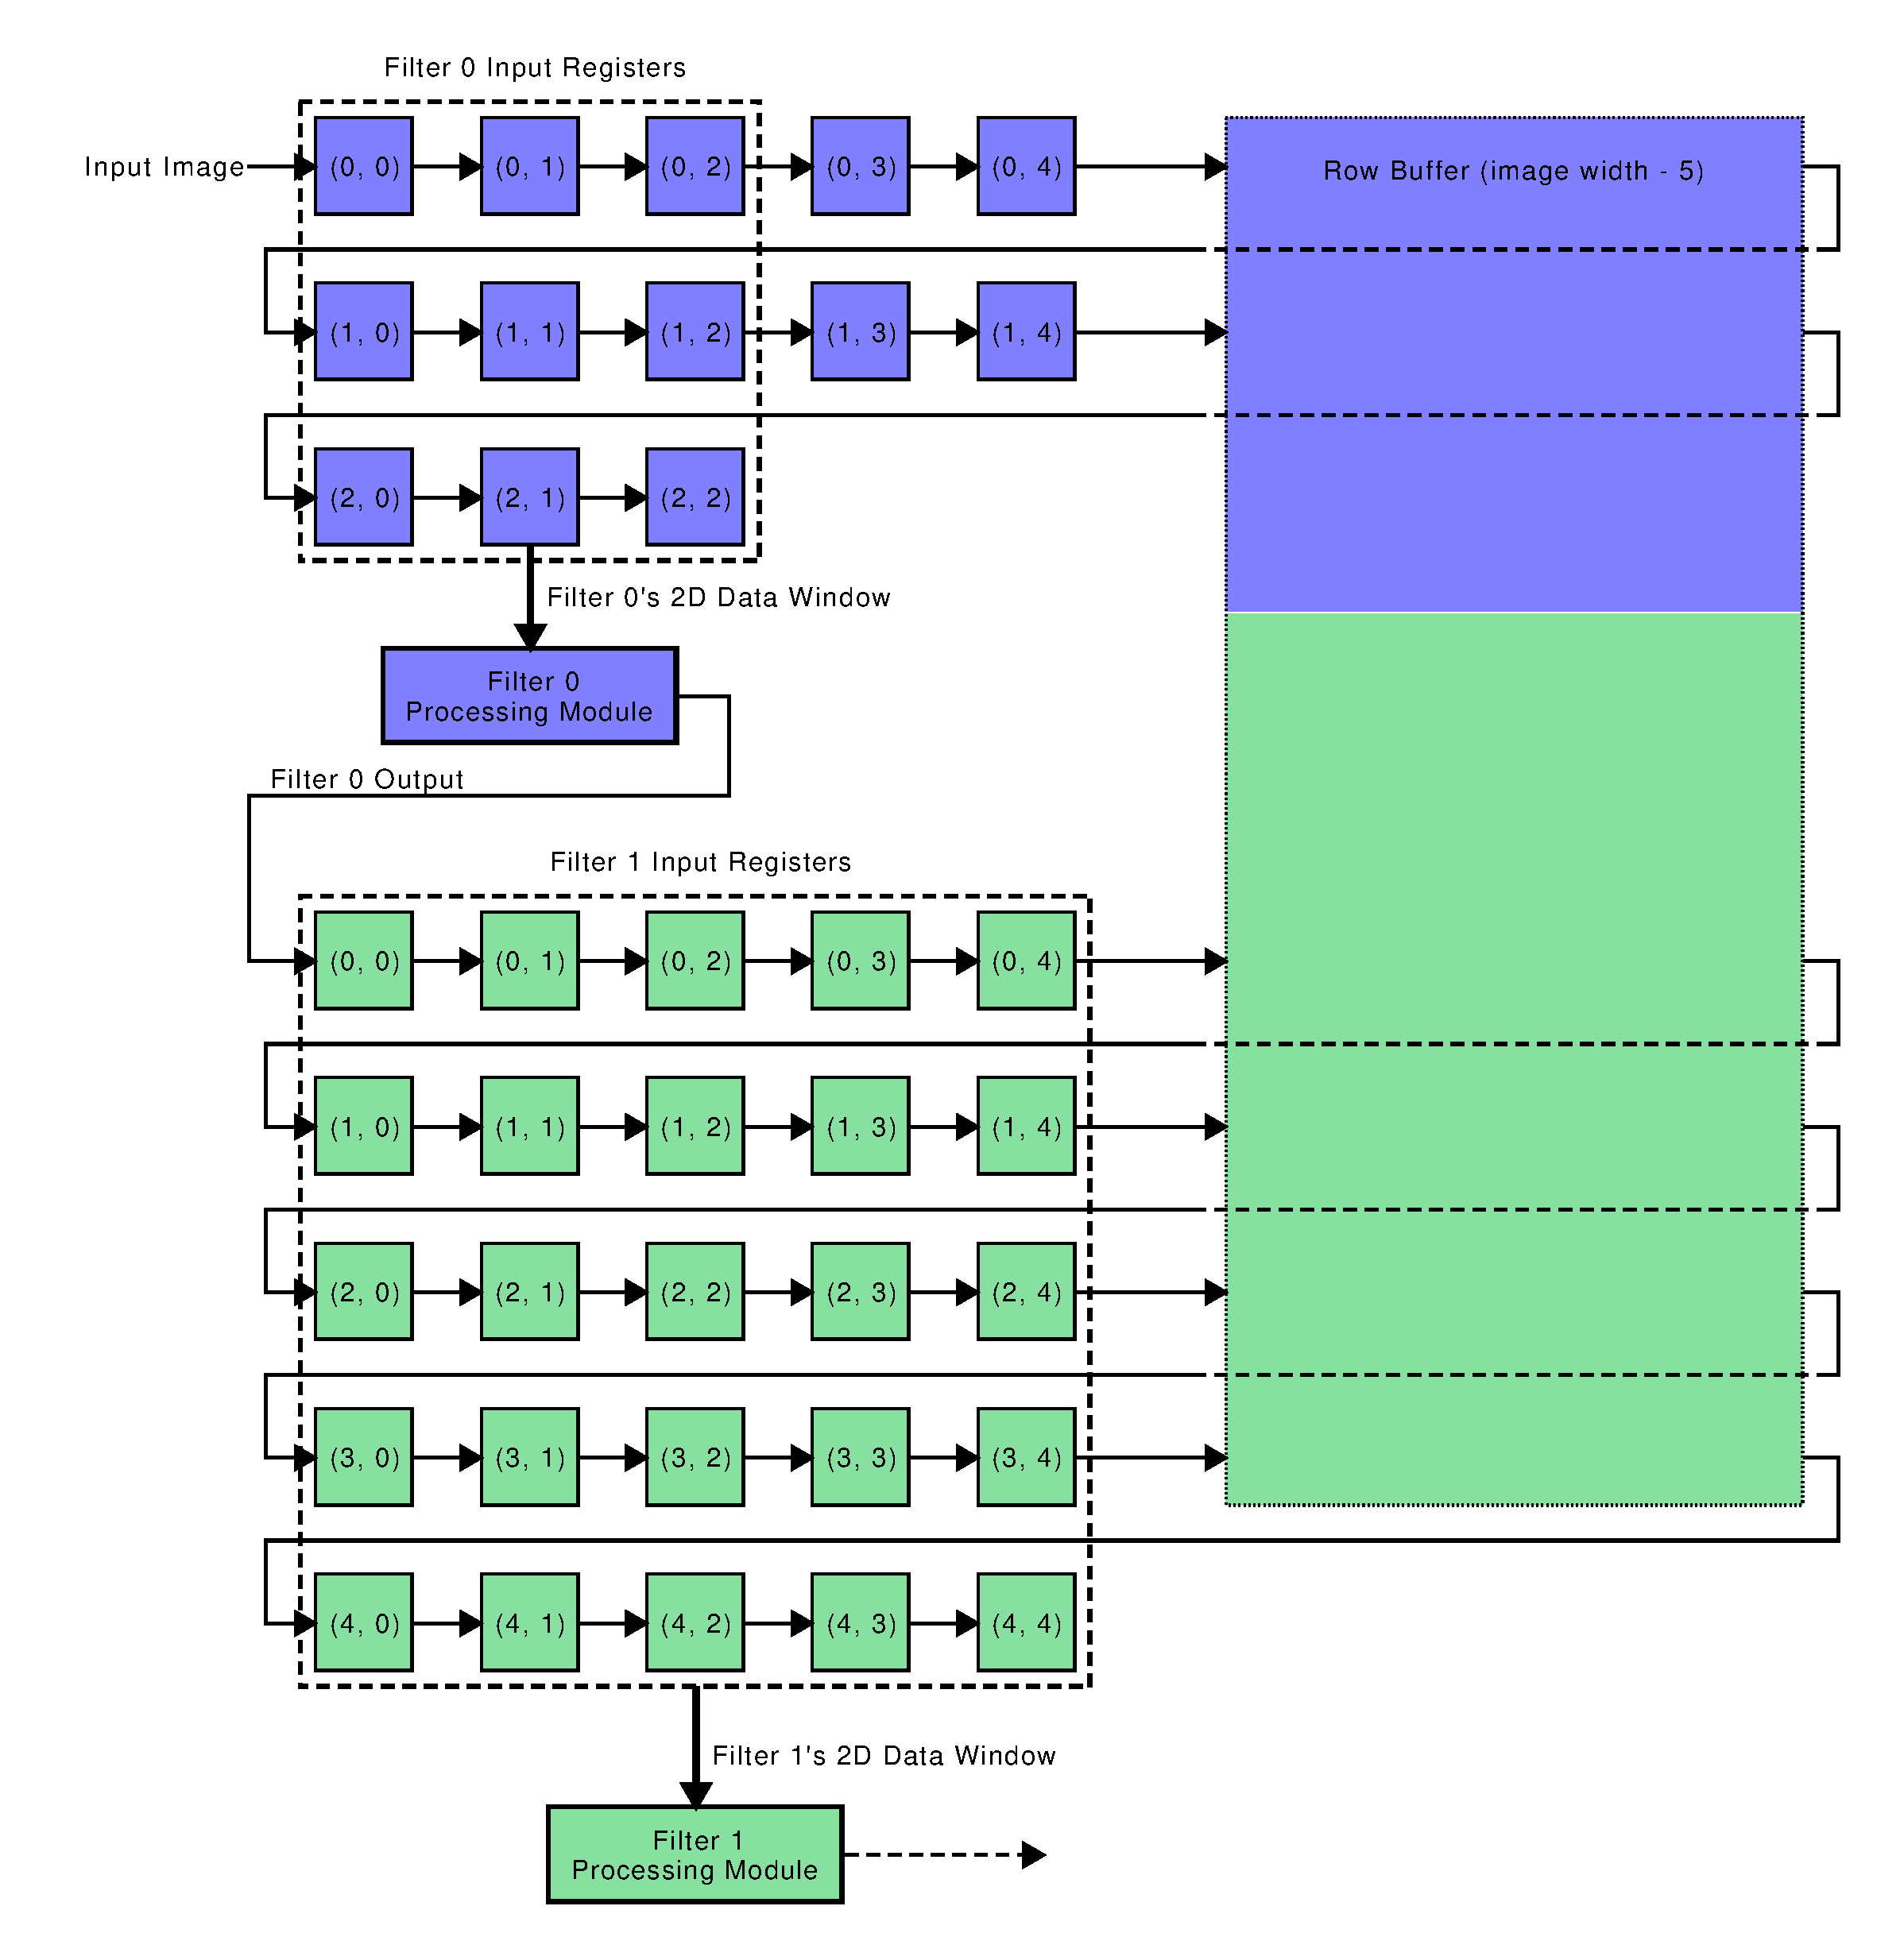
\includegraphics[width=\textwidth]{figs/02-window_buffers_opt_visual.pdf}
\caption{Two sliding window buffers optimized in the 2D Window Pipeline architecture.}
\label{fig:02-buffers_optimized}
\end{figure}

Figure \ref{fig:02-buffers_optimized} shows how two sliding window buffers for filter modules with differing window sizes can be optimized in the 2D Window Pipeline architecture.
All row buffers are merged into a single block RAM component which the synthesis toolchain can further optimize.
The filter window, implemented using registers, is extended for the smaller filter, to enable the merging of all row buffers in this case.
Using different optimization strategies available in the system generator Automatics, the optimizations automatically applied to the pipeline can be configured.


\subsubsection{2D Window Pipelines with Automatics}

Automatics can generate the hardware description code for a 2D Window Pipeline subsystem integrated into an \asterics chain.
Within the pipeline, all data signals that are part of sliding window buffers and all input signals of filter modules are analysed and tagged with delay information.
This data on pixel delays is used to automatically generate a flushing management component used to flush the pipeline when the last image data is to be extracted from it.
Further, delay information is used to generate buffers to synchronize data signals with the main image data stream that is input into the pipeline.
The placement and generation of all sliding window buffer components is fully automatic.

Some of the features of automatically generated 2D Window Pipeline systems include:
\begin{itemize}
\item Fully automatic buffer generation and optimization.
\item Configurable buffer optimization strategies.
\item Arbitrarily shaped filter windows are supported.
\item Automatic generation of synchronization buffers for input signals.
\end{itemize}

Some limitations apply to automatically generated 2D Window Pipeline systems:
\begin{itemize}
\item No border management. The outer pixels will be invalid data.
\item Only a single output per pipeline. Only the output with the highest pixel delay will be correctly handled by the pipeline data management component.
\item No user adjustable delays. Individual signals or modules cannot currently be adjusted in their delay and therefore their logical placement in the pipelines data streams.
\end{itemize}


\subsubsection{Creating a 2D Window Pipeline Subsystem}

To create a 2D Window Pipeline using Automatics use the following command \emph{after} having created a chain object:
\begin{lstlisting}[style=AutomaticsPython]
import asterics
chain = asterics.new_chain()
# Chain object created, now pipelines can be created
pipe = asterics.new_2d_window_pipeline(640)
\end{lstlisting}

The command \lstapyinline{asterics.new_2d_window_pipeline(width, height, name)} can be provided with three parameters.
The width of the image that the pipeline will process is mandatory.
The second parameter, the height of the image is optional and currently not used.
The third parameter can be used to name the pipeline.
For each pipeline a separate VHDL file will be generated, using the name provided.
If no name is provided the pipeline will be named \texttt{as\_window\_pipeline\_<num>}, replacing the \texttt{<num>} placeholder with the number of pipelines in the system.
Similar to the \lstapyinline{asterics.new_chain()} and \lstapyinline{chain.add_module()} commands, this command also returns the object that it creates, assigning it to the keyword (variable) provided to the left of the equals sign.
We recommend using a variable name along the lines of \lstapyinline{pipe}, which will be used in this manual to refer to a 2D Window Pipeline object.

The pipeline has a few advanced configuration options, mostly relating to the optimization of automatically inserted data buffer components, that can be set.
These options have sensible defaults, generally not requiring modification.
For detailed information on these configuration parameters, refer to section \ref{sec:06-02-2dpipe_general}.


\subsubsection{Window Modules of 2D Window Pipeline Subsystems}

A window module is an \asterics module with a special \textbf{Window Port}.
This port in conjunction with other standardized ports are collectively referred to as a \textbf{Window Interface}, as detailed in section \ref{05-04-as_2d_window_filter_signals}.
Window modules differ from regular modules, also referred to as \textbf{Streaming Modules}, mainly by the inclusion of a window interface.
To be used with Automatics correctly, window modules require a special module specification script, declaring the module as a window module, for details refer to section \ref{sec:06-02-custom_window_modules}.
By declaring a module as a window module to Automatics, it may only be used in a 2D Window Pipeline subsystem.
In a pipeline, special connection rules apply to standard ports of window modules, to correctly integrate the window module into the hardware architecture of the pipeline.

\subsubsection{Adding, Configuring and Connecting Window Modules}

In general, only window modules can be used within 2D Window Pipeline subsystems.
To add a window module to the pipeline, the same command used with the \lstapyinline{chain} object is used:\\
\lstapyinline{pipe.add_module("module name", "user name", "repository")}\\
The parameters of the command are also the same as when used with a \lstapyinline{chain} object.
For example:\\
\lstapyinline{gauss_filter = pipe.add_module("as_2d_conv_filter_internal", "fgauss")}

Furthermore, all configuration commands available, including those discussed in section \ref{ssec:02-configuring} work for window modules.

To connect window modules with each other, the \lstapyinline{connect()} command can be used as described in section \ref{ssec:02-connecting}, however, for window interfaces and ports and when connecting into and out of the pipeline, special rules have to be followed, as detailed in section \ref{sec:06-02-2dpipe_general}.

The following chain description script excerpt serves as an example of two window modules being added, configured and connected within a pipeline:
\begin{lstlisting}[style=AutomaticsPython]
# Add a camera and memory writer to the system
camera = chain.add_module("as_sensor_ov7670")
writer = chain.add_module("as_memwriter")

# Create new 2D Window Pipeline
pipe = asterics.new_2d_window_pipeline(640, name="filterpipe")

# Add two filter modules named gauss and laplace:
gauss = pipe.add_module("as_2d_conv_filter_internal", "gauss")
laplace = pipe.add_module("as_2d_conv_filter_internal", "laplace")

# Configure generics of the window modules
gauss.set_generic_value("KERNEL_SIZE", 5)
gauss.set_generic_value("KERNEL_TYPE", '"gauss"')
laplace.set_generic_value("KERNEL_SIZE", 3)
laplace.set_generic_value("KERNEL_TYPE", '"laplace"')
laplace.set_generic_value("NORMALIZE_TO_HALF", "true")

# Connect from the camera into the pipeline to gauss
# This connection will create a sliding window buffer
# for gauss' window port
camera.connect(gauss)

# Connect the data output of gauss with the window port of laplace
# This connection will also create a sliding window buffer
gauss.get_port("data_out").connect(laplace.get_port("window_in"))

# Connect the port vsync of camera to laplace
# This connection will create a synchronization buffer,
# so the data from the vsync port will arrive synchronized 
# with the data originally from the data port of camera.
# Note: For example only, laplace does not have a suitable port here
camera.get_port("vsync_out").connect(laplace.get_port("vsync_in"))

# Connect the data output of laplace with writer
laplace.get_port("data_out").connect(writer.get_interface("in"))
\end{lstlisting}


\subsection{Neural Network Layer Subsystems}

\asterics includes generic convolution modules that are capable of computing certain layers of neural networks, more specifically convolutional neural networks (CNNs).
Convolutional layers and pooling layers can currently be implemented with \asterics.
The development of systems containing such CNN layer accelerators is supported by Automatics.

A CNN accelerator system using \asterics is build using a separate \lstapyinline{AsNNLayer} object to accelerate each layer you want to compute using \asterics.
Currently, only networks quantized using TensorFlow-Lite to 8 bit integer weights are supported.
A delegate software exists for use with TensorFlow-Lite to let the framework delegate the computation of one or multiple layers to \asterics hardware.

\begin{lstlisting}[style=AutomaticsPython]
# Create a new layer operating on a 300x300 image
layer1 = asterics.new_nn_layer(image_width=300, name="CONV2D1")
# Set layer type, weights, biases,
# quantization values and meta-parameters
layer1.parametrize_and_build(
    operation="CONV2D",
    input_bit_width=8,
    output_bit_width=8,
    kernel_size=3,
    input_channel_count=3,
    filter_count=64,
    strides=2,
    activation_function="none",
    weights_npy_file=weights_file_1,
    biases_npy_file=biases_file_1,
    quantization_factors_npy_file=operators_file_1,
    filters_per_module=4,
    quantization_offset_value=-128,
    weight_accuracy=8,
)
\end{lstlisting}

The above listing shows an excerpt of an Automatics script where a neural network layer is added to an \asterics chain and configured.
The first command, \lstapyinline{asterics.new\_nn\_layer}, creates a new layer acceleration subsystem for a specific width of image data to process.
Optionally, a name can be provided, which makes the generated code easier to read.
This method returns a layer acceleration object, just like when a new module is added or a 2D Window Pipeline subsystem is created.

The second command \lstapyinline{<layer object>.parametrize\_and\_build} takes a large number of parameters defining the exact behaviour of the neural network layer.
Some basic parameters, such as the type of operation the layer should implement (\texttt{operation}), the bit width of the data to be processed and generated (\texttt{input\_bit\_width, output\_bit\_width}) and the number of channels of the input image data (\texttt{input\_channel\_count}) must be provided.
The dimensions of the weight data must be provided for convolution layers, comprising the kernel height and width (\texttt{kernel\_size}) and the number of filters (\texttt{filter\_count}).

Furthermore, the bias, weight and quantization values are required, either in the form of a Numpy file or a direct textual form in the script.
For more and detailed information on the parameters and the generation of CNN accelerator systems with Automatics, see section \ref{sec:06-02-cnns}.


\subsection{Advanced Configuration Using Signals and Module Groups}

Automatics has the capability to handle generic VHDL signals.
Using signals is generally not required to build most systems and should only be used if necessary for advanced configurations.
This functionality is only available in the context of \textbf{Module Groups}.
Both the main VHDL file generated by Automatics, \texttt{as\_main.vhd}, representing most of the \asterics chain and the 2D Window Pipeline subsystems are represented using module groups and can make use of signals.
The module group \texttt{as\_main} can be accessed using: \lstapyinline{chain.as_main}.


To define a new VHDL signal, use the following command:
\begin{lstlisting}[style=AutomaticsPython]
chain.as_main.define_signal("name", "data type", 
                            <data width>, "fixed value")
\end{lstlisting}
For more details on the command, refer to its description in section \ref{sec:06-02-config_methods}.

As with modules, the added signals are returned by the command and can be assigned using a variable:
\begin{lstlisting}[style=AutomaticsPython]
flush = chain.as_main.define_signal("custom_flush")
\end{lstlisting}

Signals are treated much like ports of modules, that can be connected to both a source and multiple sinks.
Signals with vector types can be partially assigned from multiple ports or signals and to multiple ports and signals.
Refer to the descriptions of the commands \lstapyinline{assign_to_this_vector()}, \lstapyinline{assign_from_this_vector()} and \lstapyinline{define_vector_assignment()} in section \ref{sec:06-02-config_methods}.

As the 2D Window Pipeline subsystem is modeled using a module group, signals can also be created in pipelines.
Automatics supports creating a connection from a signal within a pipeline to the outside, creating an \texttt{as\_stream} interface with the signal as the data source.
This is useful when the outputs of multiple window modules should be bundled and output as a single signal.


\subsection{Selecting Output Products and Running the Synthesis Toolchain}
\label{ssec:02-output}

Automatics provides multiple output products.
This includes generating only the source files for the described \asterics chain, generating an IP-Core using Xilinx Vivado, and generating a system template along with the IP-Core.
Furthermore, additional output products are available, providing further information about the generated chain.

The following list provides a brief overview of the available output products and the accompanying commands for the chain description script:
\begin{itemize}
\item \lstapyinline{chain.write_asterics_core("location", <use symlinks>, <force>, <module driver dirs>)}\\
This command only generates the \asterics chain source files to the \texttt{"location"} path provided.
The parameter \texttt{<use symlinks>}, by default \lstapyinline{False} can be set to \lstapyinline{True} to link source files that are not generated for the system instead of copying them.
The parameter \texttt{<force>}, by default \lstapyinline{False} can be set to \lstapyinline{True} to allow Automatics to delete anything from the provided \texttt{"location"} path, instead of stopping the generation process. \emph{Warning:} Any files in the location are permanently deleted!
The parameter \texttt{<module driver dirs>}, by default \lstapyinline{False} can be set to \lstapyinline{True} to have Automatics generate separate directories for the software driver of each \asterics module.
\item \lstapyinline{chain.write_ip_core_xilinx("location", <use symlinks>, <force>, <module driver dirs>)}\\
This command generates the source files for the described \asterics chain and packages them to an IP-Core using Xilinx Vivado.
For this command to work, Vivado has to be installed on the system and sourced before running Automatics.
All parameters function the same as for the command \lstapyinline{chain.write_asterics_core()}.
\item \lstapyinline{chain.write_system("location", <use symlinks>, <force>, <module driver dirs>, <add vears>)}\\
This command generates and packages the source files for the \asterics chain into an IP-Core using Xilinx Vivado and additionally generates an example folder structure to use as the start of an FPGA project.
The first four parameters are identical with the command \lstapyinline{chain.write_asterics_core()}.
The parameter \texttt{<add vears>}, by default \lstapyinline{False} can be set to \lstapyinline{True} to automatically add the IP-Core of VEARS, a video output generator, included with \asterics, to the system.
\item \lstapyinline{chain.write_system_graph("output file", ..)}\\
Generate and write a graph representation of the described system to \texttt{"output file"}.
This command must be called \emph{after} a command that generates the source files for the \asterics chain.
Parameters are not explained here for brevity, refer to this commands description in section \ref{sec:06-02-config_methods} for details.
\item \lstapyinline{chain.list_address_space()}\\
This command causes Automatics to output the address space that the \asterics IP-Core will occupy and the addresses and type of all registers on the command line used to run Automatics.
This command must be called \emph{after} a command that generates the source files for the \asterics chain.
\item \lstapyinline{pipe.print_pipeline_buffer_report(<verbosity>)}\\
This command lists a summary report for the buffers required by the 2D Window Pipeline it was called from on the command line used to run Automatics.
The parameter \texttt{<verbosity>}, by default \texttt{0} can be set to \texttt{1} to additionally print a report per buffer.
This command must be called \emph{after} a command that generates the source files for the \asterics chain.
\end{itemize}

Any or all of the commands to generate output products listed above may be present in the chain description script.
To actually generate the system, at least one of \lstapyinline{chain.write_asterics_core()}, \lstapyinline{chain.write_ip_core_xilinx()} or \lstapyinline{chain.write_system()} should be present and must be positioned \emph{after} any module connection, add or configuration commands.

To run Automatics simply execute the chain description script using Python 3 on the command line.
Note that the \asterics settings file must have been sourced before Automatics can be used.
For example, for the chain description script \texttt{example-script.py}:
\begin{lstlisting}[style=shell]
 > python3 example-script.py
\end{lstlisting}

After Automatics has completed, the resulting output can be either packaged into an IP-Core manually, if you want to use a toolchain other than Xilinx Vivado, or integrated into a Vivado block-design by adding the IP-Core to the IP Catalog in Vivado.
After the IP-Core is added to the block-design and connected, synthesis may be run.

The reference designs included with \asterics provide a Makefile automating much of the manual process after running Automatics, for details refer to section \ref{sec:02-02-build-process}.

\subsection{Software Development}

In general, \asterics systems can be operated either using bare metal software, without an operating system, or using Linux.
For the operation under Linux, a kernel driver is available in \texttt{asterics/support/software/as-linux/}.
At this time, the driver has not been integrated into the generation process of Automatics and requires manual configuration.
For more information about the kernel driver, refer to section \ref{ch:04-05-software-linux}.

For bare metal operation, Automatics generates the \asterics Support Package (ASP) on a system by system basis.
The user application only has to include a single header file, \texttt{asterics.h}, to access all functionality of the hardware.
For more information on the ASP, refer to the first sections of chapter \ref{ch:04-software}.

\subsubsection{Developing a Bare Metal Application that Uses \asterics}

To gain access to all functionality of an \asterics chain integrated into the hardware, only the \texttt{asterics.h} header file has to be included in the user application:
\begin{lstlisting}[style=CStyle]
#include "asterics.h"
\end{lstlisting}

The \asterics Support Package (ASP) including the main header is located in \texttt{ASTERICS/driver/} in the IP-Core generated by Automatics or in \texttt{asterics\_core/software/} if the \asterics core output product is used.
\texttt{asterics.h} contains the include statements for driver files of the modules used in the chain, as well as the definition statements for slave register address mapping.

Before using any \asterics specific function, the function \texttt{as\_support\_init()} must be called to initialize the hardware.
Analogously, before shutdown the function \texttt{as\_support\_done()} must be called.

To develop the software, refer to section \ref{ch:04-software} for general information, and chapter \ref{ch:07-modules} for information on each of the modules used in the chain, to inform about the software interface and functions available.

\subsubsection{General Conventions of Module Drivers}

\begin{itemize}
\item In general, the functions for modules are prefixed with the module name for better readability and a clear association, for example: Functions for the module \texttt{as\_iic} are all named \texttt{as\_iic\_<function name>}.
\item Module drivers generally provide initialization functions that must be called before normal operation and configuration. They usually have \texttt{init} in their name.
\item Many functions require the module's base address of its slave registers, using the parameter \texttt{base\_addr}.
These addresses are defined in the main header file \texttt{asterics.h}.
Module base addresses are all named \texttt{AS\_MODULE\_BASEADDR\_<module name>}.
The \texttt{<module name>} is the user name of the module as defined in the chain description script.
If no user name is provided when the module is added, Automatics uses the module's entity name and concatenates a running number at the end.
\end{itemize}


\subsubsection{Hardware-Software Communication}

Every \asterics module may include a slave register interface to facilitate communication with the software.
Slave registers are used to communicate the current state of the hardware, the modules of the \asterics chain, to the software, to set configuration values that need to be changed during run-time and to control the behaviour of the modules.
To transmit large amounts of data to the hardware and vice-versa, the data should first be written to main memory, for example using the modules \texttt{as\_memwriter} and \texttt{as\_memreader} (refer to section \ref{ch:07-basic-mods-in_out}).

For all slave register interfaces of all modules in a chain, Automatics automatically generates a mapping of the registers to the address space of the target hardware.
This address space is defined by a configurable base address and its size.
These values can be defined in the chain description script to match the target hardware and system configuration, refer to section \ref{ssec:02-hwtargetconfig}.
During the mapping process, first, the module with the largest number of registers is identified.
Based on that number an address space per module is defined by the next highest power of two.
Each module is then assigned its own register space and base address.

For information on how to integrate a slave register interface into a custom hardware module, refer to section \ref{sec:05-01-05-register_interface}.


\subsubsection{Slave Registers of 2D Window Pipeline Subsystems}

Regular, streaming \asterics modules, can implement registers directly, using the slave register interface.
As window modules are part of a subsystem, the register interface may not be used in the modules directly.
Instead, each pipeline provides its own register interface.
This interface can be managed using commands in the chain description script.


By default, two registers are included with every pipeline:
A control register at index 0, providing a reset control bit at bit index 0 and a start flush control bit at bit index 1.
A status register at index 1, by default only providing a status bit at bit index 0 providing the "ready"-status of the pipeline.
Each \asterics module, the pipelines included, are assigned a number of registers, starting at index 0.
As the pipeline includes 2 registers already, any new registers, not impeded by the functionality of the default registers, meant to function as control and status register respectively, must be assigned to index 2 and higher.

Automatics provides two commands to add and modify registers of the 2D Window Pipeline:
\begin{itemize}
\item \lstapyinline{pipe.assign_port_to_register(<register number>, <port>, <bit index>)}\\
This command adds a port or signal to the register with the index \texttt{<register number>}.
If the register at index \texttt{<register number>} does not exist yet, it is created automatically.
The value of the register bits starting at bit index \texttt{<bit index>}, are then assigned by the provided \texttt{<port>}.
The number of bits of the register that are assigned by \texttt{<port>} depend on the data type of the port provided.
\item \lstapyinline{pipe.assign_register_to_port(<register number>, <port>, <bit index>}\\
This command function analogously to the command described above.
The only difference is the data direction: In this case data from the register is assigned to the port or signal provided, instead of the other way around. 
\end{itemize}

The following are examples of the commands used correctly:\\
Assign register with index 2 from bit index 0 to the port \texttt{threshold\_in} of module \texttt{ffeature}:
\begin{lstlisting}[style=AutomaticsPython]
pipe.assign_register_to_port(2, ffeature.get_port("threshold_in"), 0)
\end{lstlisting}
Assign bit 1 of register with index 1 to the value of the port \texttt{ready} of module \texttt{ffeature}:
\begin{lstlisting}[style=AutomaticsPython]
pipe.assign_port_to_register(1, ffeature.get_port("ready"), 1)
\end{lstlisting}

%\subsection{Simulating and Debugging \asterics Chains}
%\label{ssec:02-debugging}

% [MS] TODO / TBD


\subsection{Manually Modifying an \asterics System}
\label{ssec:02-manual}

Generally, it should not be necessary to manually modify the hardware source code generated by Automatics, as the tool is capable of generating most system configurations.
However, in some edge cases, it may be impossible to achieve the configuration desired using Automatics alone.
As manual modification on generated files may be necessary, the files are generated with human readability in mind.

An \asterics system consists of the following generated / modifiable hardware components:
\begin{itemize}
  \item \texttt{asterics.vhd} is the top level file of the \asterics IP-Core. It instantiates modules for master and slave bus access and the \texttt{as\_main} hardware component module.
  \item \texttt{as\_main.vhd} implements the actual image processing chain by instantiating and connecting the appropriate \asterics modules.
  	It also contains any 2D Window Pipeline hardware components included in the system, which in turn contain their respective \asterics modules.
  	These files will have the name specified for the chain description script or, if none is defined, will be called \texttt{as\_window\_pipeline\_[0-9].vhd}
\end{itemize}

\emph{Note:}
All \asterics modules included in the system are static hardware descriptions only configurable via VHDL generics.
Module hardware files must not be modified to prevent affecting other \asterics systems that are generated from or link to the same source files.
Instead, if a modification of a module is desired, the module should be copied \emph{and} renamed (the entity of the module) and then modified.



%\section{The \asterics Installation Tree}
%\begin{verbatim}
%TBD (MS/GK):
%
%- Es sollte einen "make; sudo make install"-Vorgang geben, um auf 
%  einem Linux-Host eine gewöhnliche Installation nach dem 
%  FHS-Standard, z.B. unter /usr/local oder /opt zu ermöglichen. 
%  Als nächster Schritt werden damit auch .deb-Pakete etc. möglich.
%  
%- Der Baum könnte wie folgt aussehen 
%  (<prefix> z.B. = /usr, /usr/local/ oder /opt):
%
%	<prefix>/bin:            
%       Binaries aller Tools
%	<prefix>/lib: 
%       evtl. Bibliothekten zu den Binaries
%	<prefix>/share/asterics:
%       Kopie des Teils des Source Tree, der auf dem Entwicklungs-PC
%       als Daten benötigt wird:
%       - 'ipcores', 'modules', 'support' unbedingt
%       - 'tools', 'systems' nicht
%
%- Makefile pro Modul:
%    - optional
%    - falls nicht vorhanden: beim globalen "make install" wird nach <prefix>/share/asterics kopiert
%    - falls vorhanden: 'make install' wird aufgerufen
%    - Pflicht-Target: install
%    - Optionale:: sim, syn
%    
%- Modul-spezifische Tools (z.B. UHT, NITRA): liegen im Modul-Ordner, werden mit 'make install' nach ../bin installiert
%
%
%
%\end{verbatim}
%Presently, the \asterics installation tree corresponds to the \asterics source tree since there are no installation steps needed to use the \asterics framework.\\
%This is likely to change in the near future as there's a lot of ongoing development, especially in the field of the \asterics development tools (as-builder).

%%%%%%%%%%%%%%%%%%%%%%%%%%%%%%%%%%%%%%%%%%%%%%%%%%%%%%%%%%%%%%%%%%%%%%%%%%%%%%
%%
%% This file is part of the ASTERICS Framework. 
%%
%% Copyright (C) Hochschule Augsburg, University of Applied Sciences
%% Efficient Embedded Systems Group
%%
%% Author(s): Gundolf Kiefer <gundolf.kiefer@hs-augsburg.de>
%%
%%%%%%%%%%%%%%%%%%%%%%%%%%%%%%%%%%%%%%%%%%%%%%%%%%%%%%%%%%%%%%%%%%%%%%%%%%%%%%



%%%%%%%%%%%%%%%%%%% 3. Developing ASTERICS %%%%%%%%%%%%%%%%%%%


\chapter{Developing \asterics} \label{ch:03-developing}

\secauthor{Michael Schäferling, Alexander Zöllner, Gundolf Kiefer}

\section{Organization of the GIT repositories}

The \asterics Frameworks code base is organized in a set of GIT repositories.\\
\emph{Note:} The GIT repositories mentioned here are only accessible from \emph{within the local network} of the University of Applied Sciences Augsburg.
Visit the website \texttt{\url{http://ees.hs-augsburg.de/asterics}} for access to a snapshot of the repository or visit the GitHub page linked on the website.

The \asterics GIT repository contains a subset of publicly accessible modules, systems and tools and is organized according to the source tree structure (see section \ref{ch:02-using}).
You can view the codebase online by browsing

\begin{footnotesize}
    \begin{lstlisting}[style=shell]
$ https://ti-srv.informatik.hs-augsburg.de/gitweb/?p=asterics.git
    \end{lstlisting}
\end{footnotesize}

\noindent or download it by 

\begin{footnotesize}
    \begin{lstlisting}[style=shell]
$ git clone https://ti-srv.informatik.hs-augsburg.de/repo/asterics.git
    \end{lstlisting}
\end{footnotesize}

\ifdefined\astericsinternal
\noindent The \asterics-nonfree GIT repositories contents are not publicly available, e.g. due to copyright or other reasons. 
Its directory structure conforms to the source tree structure (see section \ref{ch:02-using}). 
In order to be able to make use of the contents of the (free) \asterics GIT repository, it is included as a submodule (in 'external/asterics') with its contents being sym-linked to the \asterics-nonfree GIT repositories source tree. 
If you are authorized, you can get the codebase by 

\begin{footnotesize}
    \begin{lstlisting}[style=shell]
$ git clone \
https://ti-srv.informatik.hs-augsburg.de/repo/asterics-nonfree.git
    \end{lstlisting}
\end{footnotesize}

\noindent Additionally, the are GIT repositories for specific projects, research activities or studies, which may also include \asterics(-nonfree) GIT repositories.
\fi

\section{License and Copyright}


This document and the mentioned download link refer to the free and publicly available part of ASTERICS. This part is generally licensed under the LPGL (see the LICENSE file in the root folder of the repository for details).

However, there are more ASTERICS modules available, which are presently not published under an open source license, but that can be made available individually on a per-project basis. These include modules for:
\begin{itemize}

\item the Generalized Hough Transform and other variants of the Hough Transform \cite{kiefer_configurable_2016}, \cite{hough_object_recog}

\item low latency lense distortion removal and stereo rectification (NITRA) \cite{nitra_paper0}, \cite{nitra_paper1}

\item efficient, on-the-fly point feature extraction (SURF algorithm) \cite{pohl_efficient_2014}
\end{itemize}

Please contact the Efficient Embedded Systems (EES) group at the University of
Applied Sciences Augsburg (see "authors" section on top of the file) for
further information on using these modules and collaborating with the EES group.

If you add something to the project that is licensed under a different license, please append to the LICENSE file.
Make sure that the license you are using is compatible with the LGPL.

\bigskip

\textit{Acknowledgments:}\linebreak
Parts of this work have been supported by the German Federal Ministry for
Economic Affairs and Energy (BMWi), grant number ZF4102001KM5 (2015-2018).

Parts of this work have been supported by the German Federal Ministry of
Education and Research (BMBF), grant number 17N3709 (2009-2013).

\section{The \asterics Source Tree}
\label{sec:02-file_structure}
The \asterics source tree consists of the following elements:
\begin{itemize}
  \item \texttt{doc}: Documentation directory. The output of Doxygen and the PDF of this manual are generated here
  \item \texttt{doc-src}: Documentation source files, including this manual and Doxygen \texttt{doxyfile}s to generate full code documentation 
  \item \texttt{ipcores}: IP-Cores which are part of the \asterics project
  \item \texttt{modules}: Image processing, data management and supporting modules. A separate subfolder should be created for each module or groups of similar modules.\\
  Each subfolder contains: 
  \begin{itemize}
  	\item \texttt{/doc}: Additional documentation for the module
  	\item \texttt{/hardware/automatics}: Module specification scripts for the system generator Automatics 
  	\item \texttt{/hardware/hdl}: Hardware source files of the module
  	\item \texttt{/software}: Software driver for the module
  \end{itemize}
  
  \item \texttt{support}: \asterics support files (including base for \asterics software support package 'ASP')
  \item \texttt{systems}: Small ready-to-use systems with preconfigured core structures
  \item \texttt{tools}: Supporting tools (e.g. Automatics)
\end{itemize}

\section{Contributing Modules to \asterics}

This section provides guidance for developers who want to integrate an existing or new hardware or software module into the \asterics framework.


\begin{enumerate}

\item
For new and existing modules alike, make sure that the VHDL entity of you module's toplevel file follows the coding rules laid out in section \ref{sec:06-02-vhdl_quirks}.

\item
If your module should be able to easily interface with other existing \asterics modules, you should make use of the existing interfaces used in the framework, presented in section \ref{ch:05-interfaces}.

Optionally, you may create an interface definition for your own interface and integrate it into Automatics, as described in section \ref{sec:06-02-new_interface_template}.
This allows Automatics to recognize the interfaces of your modules and enables it to connect them more simply using Automatics scripts.

Alternatively, a separate module, converting between interfaces used by existing modules and common interfaces of \asterics modules, could also prove to be a simpler solution, than editing multiple modules to conform to \asterics interfaces.

\item
The source files, both hardware and software, should be integrated either into the \asterics source tree or into a separate module repository mimicking the folder structure of the \texttt{modules} folder of the \asterics source tree, shown in section \ref{sec:02-file_structure}.
Separate module repositories are encouraged as it keeps the \asterics repository clean and allows for a clear distinction between \asterics native modules and external modules.
Automatics enables the inclusion of external repositories using a single method call in Automatics scripts, see \lstapyinline{asterics.add_module_repository()} in section \ref{ssec:06-02-asterics_pymodule}.

\item 
For each module that you want to be individually configurable and accessible by Automatics, a separate specification Python script must be created.
This process is described in section \ref{sec:06-02-new_modules}.

\item
We recommend to double-check that your module is correctly imported by Automatics using the \asterics GUI.
If all ports, generics, interfaces and files are recognized, you can use the module in the same way as any other module in Automatics scripts.

\end{enumerate}





\section{Coding Conventions}

%%%%%%% Begin of document %%%%%%%


\subsection{C Code}

\secauthor{Michel Zink}

\subsubsection{Introduction}\label{C-Introduction}

This chapter defines rules and requirements for maintaining and developing C source code for the \asterics framework. The main emphasis hereby lies on the style and coding conventions of C source code itself, files- and directory-naming included.

The purpose of this section is to enable good comprehensibility of the developed C source code across various software developers and increase its general quality.
Thus, reducing the initial time required for acquiring understanding of a given source code and simplify its maintenance as well as accelerate the integration of new newly developed functionalities into the \asterics framework.

The given requirements outlined in this document are based on the C99 standard as common ground.

This chapter uses the expressions \textit{must/has to}, \textit{strongly recommended}, \textit{should} and \textit{can} to give information about the relevance of the coding convention in question.
Rules or sections marked as \textit{must} are binding and are to be applied without exception.
\textit{Strongly recommended} parts are to be always applied unless there is a valid reason for this rule being circumvented.
Sections using the expression \textit{should} are considered good practice and usually improve the quality of the code.
However, software developers are not obliged to conform to this kind of rule but are encouraged to do so.
The least restrictive expression used in this document is \textit{can}.
These parts generally provide only suggestions or general guidelines which may be applied.
Software developers are free to choose equivalent or different rules for the sections marked as \textit{can}. 


\subsubsection{General Requirements}\label{C-General-Requirements}

All file names, comments, code and documentation must be written in English or have to be based on the English language. Further, only letters a-z, the underscore character \_ or numerals 0-9 must be used.

For enabling compiler independent code, utilization of common language construct are strongly recommended.

The line length of the code should be limited to 80 characters as much as possible. Longer lines tend to be more difficult to read. For this reason, it is strongly recommended to only use a single statement in each line.

Only \textit{soft tabulators} (i.e. a sequence of single white spaces) must be used instead of \textit{hard tabulators} (i.e. tabulator key).
The inferred space of hard tabulators are editor dependent and thus the actual indentation is likely to vary.
A sequence of single white spaces are uniformly displayed across editors.
It is strongly recommended to use a number of white spaces ranging from 2 to 4 for a single indentation.
More white spaces make it easier to find blocks in the source code but increases the overall line length.


\subsubsection{File Naming Convention}

File names are made up of a base name, and an optional period and suffix. The first character of the name should be a letter and all characters (except the period) should be lower-case letters and numbers. The base name should be eight or fewer characters and the suffix should be three or fewer characters (four, if you include the period). These rules apply to both program files and default files used and produced by the program (e.g., "foobar.sav").

In addition, it is conventional to use Makefile (not makefile) for the control file for make (for systems that support it) and "README" for a summary of the contents of the directory or directory tree.


\subsubsection{Documentation}\label{C-Documentation}

\paragraph{General:}
All developed source code has to contain appropriate comments to simplify maintenance and to reduce the required time for other software developers to understand the code. For this reason, meaningful comments have to be written which clearly state the purpose of the following code instead of repeating the code in textual form (e.g. This is an assignment). The following sections cover the parts of the software which require comments. Further comments can be added as seen fit.

\paragraph{Doxygen:}
Variables and function prototypes should be commented with a doxygen compatible comment syntax to easily create a class documentation for the project. The syntax looks like:
\begin{verbatim}
/// Brief description.
/** Detailed description. */
\end{verbatim} 

\paragraph{Standard Top Comment:}
Each source file must contain a standardized comment at the start of the file, which contains important information. \ref{CHEADER} shows the structure of an exemplary header comment. The author must provide information for each entry (marked with \textless\textgreater). The \textit{Modified} entry has to be updated each time something has been changed on the current version of the module. Each file has to contain information about the license for this file. Since \asterics is an open framework, \textit{GNU GPL} is the most common license, however, a different license can be chosen.

\begin{lstlisting}[style=CStyle, label=CHEADER, caption=\asterics C source file header]
/**
----------------------------------------------------------------------
--  This file is part of the ASTERICS Framework. 
--  (C) <year> Hochschule Augsburg, University of Applied Sciences
----------------------------------------------------------------------
-- File:           <file_name>.c/h
--
-- Company:        Efficient Embedded Systems Group 
--                 University of Applied Sciences, Augsburg, Germany
--                 http://ees.hs-augsburg.de
--
-- Author:         <main_author> [<year>], [<second_author> <year>]
--
-- [Modified:       <modification_author> - <year>: <description>]
--
-- Description:    <Detailed information about the purpose of this 
--                 module>
--                 
----------------------------------------------------------------------
--  <License text>
----------------------------------------------------------------------
--! @file <file_name>.c/h
--! @brief <concise description about the purpose of this module>
----------------------------------------------------------------------
*/
\end{lstlisting}


\subsubsection{Naming Conventions}

\paragraph{Pointer Declarations:}
The pointer qualifier "*" should be written at the variable name, instead of the type.
This prevents misreading when multiple variables are declared in one line like:
\begin{verbatim}
CORRECT:    char *s, *d, *o;  // All variables are pointers
WRONG:      char* s, d, o;    // Only s is a pointer
\end{verbatim}
This also affects function parameters.


\paragraph{Typedefs and Structs:}

Typedefs are an easy way of creating a synonym for data types and change them later if needed.
To identify typedefs easily, they have to be named with a \textit{"\_t"} suffix.
When using a typedef on a struct a suffix \textit{"\_s"} has to be appended to the typedef name to differentiate it from typedefs of simple data types.
Struct names without typedefs do not require the suffix, as they have to be explicitly referenced using the \textit{struct} keyword, though it is recommended to keep a consistent coding style.


\paragraph{Constants, Enumerations and Macros:}

Constants have to be added with the \textit{\#define} feature of the C preprocessor.
Symbolic constants make the code easier to read.
Defining the value in one place also makes it easier to administer large programs since the constant value can be changed uniformly by changing only the define.
The enumeration data type is a better way to declare variables that take on only a discrete set of values, since additional type checking is often available. 

Constants, Enumerations and Macros must be named with capital letters.
When the name has more than one word, the words should be separated with underscores to guarantee the readability.

\paragraph{Functions:} Words in function names have to be in written in lowercase and separated with underscores. 





\subsection{VHDL Code}

\secauthor{Alexander Zöllner}


\subsubsection{Purpose}

This chapter defines rules and requirements for maintaining and developing VHDL code for the \asterics framework. The main emphasis hereby lies on layout and naming convention of VHDL source code, files and directories involved.
Further, guidelines for VHDL modeling are covered to some extent as seen fit.

The purpose of this document is to enable good comprehensibility of the developed VHDL models across various software developers and increase its general quality. Thus, reducing the initial time required for acquiring understanding of a given VHDL model and simplify its maintenance as well as accelerate integration of newly developed VHDL models into the \asterics framework.

The given requirements outlined in this document are based on the VHDL-93 standard as common ground.

Since VHDL is the prevalent language throughout the \asterics framework, Verilog is not explicitly covered. However, similar rules are recommended.


\subsubsection{Conventions}

This chapter uses the expressions \textit{must/has to}, \textit{strongly recommended}, \textit{should} and \textit{can} to give information about the relevance of the coding convention in question.
Rules or sections marked as \textit{must} are binding and are to be applied without exception.
\textit{Strongly recommended} parts are to be always applied unless there is a valid reason for this rule being circumvented.
Sections using the expression \textit{should} are considered good practice and usually improve the quality of the code.
However, software developers are not obliged to conform to this kind of rule but are encouraged to do so.
The least restrictive expression used in this document is \textit{can}.
These parts generally provide only suggestions or general guidelines which may be applied.
Software developers are free to choose equivalent or different rules for the sections marked as \textit{can}. 

\subsubsection{General Requirements}\label{VHDL-General-Requirements}
All file names, comments, code and documentation must be written in English or have to be based on the English language.
Further, only letters a-z, the underscore character \_ or numerals 0-9 must be used.

For enabling compiler independent code, utilization of common language construct are strongly recommended.


The line length of the code should be limited to 80 characters as much as possible.
Longer lines tend to be more difficult to read.
For this reason, it is strongly recommended to only use a single statement in each line.

Only \textit{soft tabulators} (i.e. a sequence of single white spaces) must be used instead of \textit{hard tabulators} (i.e. tabulator key).
The inferred space of hard tabulators are editor dependent and thus the actual indentation is likely to vary.
A sequence of single white spaces are uniformly displayed across editors.
It is strongly recommended to use a number of white spaces ranging from 2 to 4 for a single indentation.
More white spaces make it easier to find blocks in the source code but increases the overall line length. 

\subsubsection{Name Style Rules}\label{VHDL-Name-Style}

The following table~\ref{Mandatory_Identifier} shows the requirements on identifiers used in the \asterics framework.
Using meaningful non-cryptic identifiers are strongly recommended.
Except for \textit{generics}, all identifiers have to be written in lower case, using the underscore character for separation to increase readability.
Camel case must not be used. 

\begin{longtable}[ht]{|c|c|c|}
\hline 
\textbf{Description} & \textbf{Extension} & \textbf{Example}\\
\hline
\hline
\endhead

\texttt{General Signal} & prefix s\_ & s\_load\_address \\
\hline
\texttt{Signal Inferring Register} & prefix r\_ & r\_memory\_addr \\
\hline
\texttt{Constants} & prefix c\_ & c\_bit\_per\_pixel \\
\hline
\texttt{Types} & suffix \_t & filter\_t \\
\hline 
\texttt{Generics} &  & DIN\_WIDTH \\
\hline 
\texttt{Keywords} &  & downto \\
\hline 
\texttt{Low Active Signal or Variable} & suffix \_n & s\_reset\_n \\
\hline 
\caption{Mandatory extensions used for signals, constants, ...}\label{Mandatory_Identifier}
\end{longtable}

The following table~\ref{Optional_Identifier} gives a recommendation for the naming convention of ports.
If a given port has a counterpart with a different direction, the corresponding identifier has to be used (e.g. data\_in, data\_out). 

\begin{longtable}[ht]{|c|c|c|}
\hline 
\textbf{Description} & \textbf{Extension} & \textbf{Example}\\
\hline
\hline
\endhead

\texttt{Input Port} & suffix \_in & data\_in \\
\hline 
\texttt{Output Port} & suffix \_out & data\_out \\
\hline 
\texttt{In/Out Port} & suffix \_inout & sda\_inout \\
\hline 
\caption{Recommended extensions used for ports}\label{Optional_Identifier}
\end{longtable}


The software developer is strongly encouraged to use meaningful labels for all sequential blocks, such as process or generate statements.
Table~\ref{Blocks} shows the identifier for the corresponding labels. 

\begin{longtable}[ht]{|c|c|c|}
\hline 
\textbf{Description} & \textbf{Extension} & \textbf{Example}\\
\hline
\hline
\endhead

\texttt{Process} & prefix p\_ & p\_data\_counter \\
\hline
\texttt{Generate} & prefix gen\_ & gen\_instantiate\_counters \\
\hline
\texttt{Loop} & prefix l\_ & l\_sample\_input \\
\hline 

\caption{Label prefix for process, generate, ...}\label{Blocks}
\end{longtable}


The entity name has to use the prefix \textit{as\_} if the corresponding module is meant to be used in an \asterics IP core. 

The architecture name has to be \textit{behavior}, \textit{structure}, \textit{rtl} or \textit{testbench} according to the content of the architecture.
It is possible for an entity to contain more than one architecture.
In this case, the architecture name has to be extended by a meaningful identifier (e.g. rtl\_sim, rtl\_synth).

All source files of a module which are related to the \asterics framework have to start with the prefix \texttt{as\_} if they are meant to be used in an \asterics \textit{IP core}.
Further, the file name has to contain a short description of the purpose of the module.
If the module instantiates submodules, the submodule is strongly recommended to contain the name of the module in its name.
The following example~\ref{Code:FILE_NAMES} shows some modules with their corresponding files.
In this case the indented names are submodules to the previous module.
Since \texttt{as\_memreader} and \texttt{as\_memwriter} both use the same submodule, the submodule does not contain \textit{reader/writer} in its name.
VHDL files must have the ending \textit{.vhd} or \textit{.vhdl}. 

\begin{lstlisting}[style=hdl, label=Code:FILE_NAMES, caption=\asterics module file names]
as_invert.vhd
as_nitra.vhd
	as_nitra_ctrl_unit.vhd
as_memreader.vhd
	as_mem_address_generator.vhd
as_memwriter.vhd
	as_mem_address_generator.vhd
\end{lstlisting}

A testbench file has to be named after the module which is tested. If more than one module is tested, the name of the top-level module has to be chosen. Testbench files have to be suffixed with \textit{\_tb}.

Package files must contain the prefix \textit{as\_}, the suffix \textit{\_pkg} and the package name has to match the file name containing the package without the file type extension. 


\subsubsection{Documentation}\label{VHDL-Documentation}
All developed source code has to contain appropriate comments to simplify maintenance and to reduce the required time for other software developers to understand the code.
For this reason, meaningful comments have to be written which clearly state the purpose of the following code instead of repeating the code in textual form (e.g. "This is an assignment").
The following sections cover the parts of the software which require comments.
Further comments can be added as seen fit.

Important code sections require a doxygen compatible comment syntax, which consists of \textit{--!}. 

Each source file must contain a standardized header, which contains important information about the file.
The following code snippet~\ref{Code:HEADER} shows the structure of an exemplary file header.
The author must provide information for each entry (shown as $\langle\ \rangle$).
Each file has to contain information about the license for this file.
Since \asterics is an open framework, \textit{GNU LGPLv3} is the most common license, however, a different license can be chosen.

\begin{lstlisting}[style=hdl, label=Code:HEADER, caption=\asterics header file]
---------------------------------------------------------------------
--  This file is part of the ASTERICS Framework. 
--  (C) <year> Hochschule Augsburg, University of Applied Sciences
---------------------------------------------------------------------
-- File:           <file_name>.vhd
-- Entity:         <entity_name>
--
-- Company:        Efficient Embedded Systems Group
--                 University of Applied Sciences, Augsburg, Germany
--                 http://ees.hs-augsburg.de
--
-- Author:         <main_author>, [<second_author>]
--
-- [Modified:      <modification_author> - <date>: <description>]
--
-- Description:    <Detailed information about the purpose of this 
--                 module>
--                 
---------------------------------------------------------------------
--  <License text>
---------------------------------------------------------------------
--! @file <file_name>.vhd
--! @brief <concise description about the purpose of this module>
---------------------------------------------------------------------
\end{lstlisting}

The description of the entity has to be partially covered in the file header by describing the purpose of the module.
The entity section has to contain comments for each generic and port by describing their purpose.
If ports can be grouped to a common interface, it is sufficient to name the corresponding interface.
The following code~\ref{Code:ENTITY} shows exemplary comments for the as\_invert module.

\begin{lstlisting}[style=hdl, label=Code:ENTITY, caption=\asterics entity comments]
entity as_invert is
    generic (
        -- Width of the input and output data port
        DATA_WIDTH : integer := 8
    );
    port (
        clk         : in  std_logic;
        reset       : in  std_logic;
        ready       : out std_logic;

        -- AsStream in ports
        vsync_in      : in  std_logic;
        vcomplete_in  : in  std_logic;
        hsync_in      : in  std_logic;
        hcomplete_in  : in  std_logic;
        strobe_in     : in  std_logic;
        data_in       : in  std_logic_vector(DATA_WIDTH - 1 downto 0);
        data_error_in : in  std_logic;
        sync_error_in : in  std_logic;
        stall_out     : out std_logic;

        -- AsStream out ports
        vsync_out      : out std_logic;
        vcomplete_out  : out std_logic;
        hsync_out      : out std_logic;
        hcomplete_out  : out std_logic;
        strobe_out     : out std_logic;
        data_out       : out std_logic_vector(DATA_WIDTH - 1 downto 0);
        data_error_out : out std_logic;
        sync_error_out : out std_logic;
        stall_in       : in  std_logic;

        --! Slave register interface:
        --! Control registers. SW -> HW data transport
        slv_ctrl_reg   : in slv_reg_data(0 to 0);
        --! Status registers. HW -> SW data transport
        slv_status_reg : out slv_reg_data(0 to 0);
        --! Aquivalent to a write enable signal
        slv_reg_modify : out std_logic_vector(0 to 0);
        --! Slave register configuration table.
        slv_reg_config : out slv_reg_config_table(0 to 0)
    );
end as_invert;
\end{lstlisting}

Blocks, such as \textit{generate} statements, or processes must be preceded by a comment section, which gives detailed information about the purpose of the following code.
The following code~\ref{Code:PROCESS} shows comments for a process which detects a synchronization error inside the module.
The first three lines are optional, however, grouping logical units and precede them with a distinctive comment makes it easier to find them.

\begin{lstlisting}[style=hdl, label=Code:PROCESS, caption=Exemplary comment for process]
---------------------------------------------------------------------
-- Process for Detecting Synchronization Error
---------------------------------------------------------------------
    --! A sync_error is detected when a strobe is received despite 
    --  the fifo buffer 
    --! being full. The error can only be lifted by resetting the 
    --  memwriter.
    p_sync_error : process(clk)
    begin
        if rising_edge(clk) then
            if reset = '1' or s_reset_soft = '1' then
                s_sync_error <= '0';
            else
                if strobe_in = '1' and s_fifo_full = '1' then
                    s_sync_error <= '1';
                end if;
            end if;
        end if;
    end process;
\end{lstlisting}

State machines are a special type of data processing and usually comprises one or more processes.
For this reason, each state of the state machine has to be commented individually by describing its purpose and listing the condition(s) to be met to transition to the following state.
The following code~\ref{Code:STATE} shows the comment section for the \texttt{s\_idle} state of the \texttt{as\_memwriter} state machine. 

\begin{lstlisting}[style=hdl, label=Code:STATE, caption=Exemplary comment of a state]
        --! Default state of as_memwriter if hw module is ready 
        --! for receiving order to conduct writing memory data.
        --! During idle state config parameters are continuously 
        --! copied into shadow registers to begin memory access 
        --! right away after receiving "go" signal. The state 
        --! machine transitions to "s_init" after receiving a 
        --! "go" signal.
            when s_idle =>
                s_mem_sm_done <= '1';
                s_mem_sm_save_config_reg <= '1';
                if s_mem_sm_go = '1' then
                    mem_sm_next_state <= s_init;
                end if;
\end{lstlisting}

Adding comments for declaration of signals, variables and constants is strongly recommended to make their purpose transparent.
Further, related declarations should be grouped together to make it easier to find them.
The following code~\ref{Code:STATE2} shows signal declarations of the \texttt{as\_iic} module. 

\begin{lstlisting}[style=hdl, label=Code:STATE2, caption=Exemplary comment for a declaration]
  --! Used to locally store the "scl_div" signal and compare with 
  --  "r_scl_counter"
  signal r_scl_div_local : std_logic_vector(SCL_DIV_REGISTER_WIDTH-1 
                                            downto 0);  
  
  --! A counter running with the system clock, as long as 
  --  "enable_sclcntr" is high
  signal r_scl_counter : std_logic_vector(SCL_DIV_REGISTER_WIDTH-1 
                                          downto 0);
\end{lstlisting}

Assignments are strongly recommended to be accompanied by appropriate comments to indicate the purpose of the statement.
A tolerated exception is so-called \textit{glue logic} between modules, which is used to map in and out ports between modules.
The comments for glue logic may be omitted.
The following code~\ref{Code:ASSIGNMENT} shows exemplary comments for signal assignments. 

\begin{lstlisting}[style=hdl, label=Code:ASSIGNMENT, caption=Exemplary comment for an assignment]
---------------------------------------------------------------------
-- Status Information for Hardware
---------------------------------------------------------------------
-- Signal previous hardware module being ready for operation
    ready           <= not s_mem_sm_busy;
-- Signal other hardware modules that a sync error has been detected
    sync_error_out  <= s_sync_error;
\end{lstlisting}


\subsubsection{Generator specific conventions}

The \asterics chain generator \textit{as-automatics} is used to analyse part of the VHDL files of \asterics modules.
To make sure that as-automatics can precisely identify the modules ports and generics, certain naming conventions should be followed:

\begin{itemize}
\item Port and generic name fragments should be delimited using underscores '\_'
\item When implementing an interface, such as \texttt{as\_stream}, the interface port names must be used
\item When multiples of the same interface is implemented, the port names must be differentiated using suffixes or prefixes, delimited using underscores
\item When implementing custom ports, names matching interfaces used in \asterics should be avoided to mitigate false positives from Automatics. Alternatively, different delimiters may be used, keeping the generator from fully parsing the port name, effectively avoiding false positives.
\end{itemize}

Port name examples:

\begin{itemize}
\item \texttt{activity}: Unproblematic name for a custom port
\item \texttt{activity\_strobe\_out}: Possible false positive, \texttt{as\_stream} uses a port named \texttt{strobe}! The name fragments are correctly delimited using underscores, which allows the generator to parse and compare the name.
\item \texttt{activity-strobe-out}: Less problematic, the generator will not be able to extract the name fragment \texttt{strobe}, which might cause a false positive.
\end{itemize}

\subsection{Python Code}

\secauthor{Philip Manke}

This section briefly outlines the coding style and rules for Python code within the \asterics Framework.
All code \textit{must} be compatible with Python version 3.5. Python 2 must not be used. 

\subsection{Coding Style Guidelines}

All Python code within \asterics should follow the conventions described in PEP 8 released on Python.org:
\url{https://www.python.org/dev/peps/pep-0008/}.

Where necessary or to increase the readability of short sections of code, rules described in PEP 8 may be purposefully broken.
Specifically the line length limit may be longer than 80 characters, as long as it is consistent within a (sub-) project.
We recommend to keep the line length within 80 characters as a general rule.
When it helps with readability of the code, longer lines are permitted.
Lines longer than 120 characters should always be avoided.
Before checking code into the Git repositories, developers should run a code formatter like \texttt{autopep8}, \texttt{black} or similar.

\subsection{Documentation}

Python code documentation in \asterics is automatically generated using Doxygen.
Additionally, we encourage users to make use of the built-in Python features using documentation strings (docstrings).

\subsubsection*{Python Docstrings:}

Developers should write docstrings for the following constructs:
\begin{itemize}
\item Every Python class
\item Any method or function that is sufficiently complex that its behaviour cannot be guessed from its name alone
\item Any highly important class variable (especially if it observes complex behaviour) 
\end{itemize}

Any method, function, class or variable which should be used by users of \asterics, for example in the case of Automatics scripts, must be especially thoroughly documented.


\subsubsection*{Doxygen:}

To allow Doxygen to generate a more helpful documentation, developers should use some additional features of Doxygen.
We suggest to manage the code by creating groups (Doxygen modules) and adding each class, function and method to one or more classes, unless they are standard methods (such as \lstapyinline{__str__()}).

The following listing shows an example of code a documented with both docstrings and Doxygen groups:

\begin{lstlisting}[style=AutomaticsPython]
##
# @defgroup example_group Doxygen Python Examples
# These classes and methods show how to use Doxygen with Python code!

## @ingroup example_group
class ExamplePythonClass:
  """! @brief Class showing documentation best practices.
  This docstring describes the class "ExamplePythonClass".
  This class shows how we expect Python code to be documented within
  the ASTERICS project.
  This class does nothing functionally."""

  ## This adds everything between @{ and @} to example_group
  # @addtogroup example_group
  # @{
  
  def demand_cake(self, cake_amount):
    """! @brief Returns the amount of cake demanded.
    @param cake_amount  The amount of cake you demand.
    @return The demanded amount modified by 'cake_size'.
    @note The cake is a lie."""
  	return self.cake_size * cake_amount

  def set_cake_size(self, size):
    """! @brief Set cake_size to a new value."""
    self.cake_size = size
    
  ## @} (addtogroup)
\end{lstlisting}

Doxygen commands are used in code comments.
Only comments started with two hash-signs (\texttt{\#}) are parsed by Doxygen, including all comments in lines below until a non-comment line is reached, as shown in lines 1 to 3.
Furthermore, Doxygen commands can also be used within docstrings, if an exclamation mark (\texttt{!}) is added to the beginning triple quotation marks, as seen in line 7.
Doxygen commands are prefixed with an at-sign (\texttt{@}) or a backslash.
Docstrings are included as part of the documentation generated for each class, method and function.
However, we recommend to always use the Doxygen legible docstring format as shown in the code example above.
This generates a more legible documentation and allows the use of the \texttt{@brief} Doxygen tag, which we highly encourage the use of.

The organization of code by function into Doxygen groups provides an additional way for new contributors to the project to explore the code using the Doxygen documentation.
Lines 1 to 3 show how a group is created.
The text in line 3 is used as the description of the group.
Line 5 shows the command to add a single member to a group, while lines 13 to 15 and 28 show the commands used to add multiple members to a group.

Within the docstring typical Doxygen tags and commands can be used to generate a documentation that is both legible as plain text and nicely formatted in the generated Doxygen documentation.
Lines 18 to 21 show an example for the method \texttt{demand\_cake}.

A method as simple as \texttt{set\_cake\_size} in line 24 does not necessarily require documentation, though a docstring with a single \texttt{@brief}, as shown here, can help in confirming the functionality already described by the method's name.
This establishes certainty as to the code's (intended) functionality in developers working with it. 

\subsection{File Structure}

Each Python file must include a standardized header, a template of which is available here, in listing \ref{lst_python_header}.
Everything marked with pointy brackets (\texttt{< >}) must be replaced by values for the respective file.
Parts marked in square brackets (\texttt{[ ]}) are optional and may be omitted.
This header is somewhat redundant to provide information using both Python's built-in docstrings and Doxygen.


\begin{lstlisting}[style=AutomaticsPython, caption={Template for the standard header of a python source file.}, label=lst_python_header]
# --------------------------------------------------------------------
# This file is part of the ASTERICS Framework.
# (C) <year> Hochschule Augsburg, University of Applied Sciences
# --------------------------------------------------------------------
"""
<filename>.py

Company:
Efficient Embedded Systems Group
University of Applied Sciences, Augsburg, Germany
http://ees.hs-augsburg.de

Author:
<author> [<year>][, <second author> <year>]

[Modified:]
[<author> - <year>: <modification>]

Description:
<description of the module/class purpose and functionality>
"""
# --------------------- LICENSE --------------------------------------
#
# <license text here>
#
# --------------------- DOXYGEN --------------------------------------
##
# @file <filename>.py
# @author <main author[s]>
# @brief <concise description>
# --------------------------------------------------------------------
\end{lstlisting}

In general each Python file should only include a large class, multiple smaller classes, only class-independent functions or constant values.
Typically, a Python file should contain less than 1000 lines of code.
Developers should use typing hints, where applicable, for example:
\lstapyinline{def example_function(number: int, text: str) -> bool:}

\part{Reference Guide}

%%%%%%%%%%%%%%%%%%%%%%%%%%%%%%%%%%%%%%%%%%%%%%%%%%%%%%%%%%%%%%%%%%%%%%%%%%%%%%
%%
%% This file is part of the ASTERICS Framework. 
%%
%% Copyright (C) Hochschule Augsburg, University of Applied Sciences
%% Efficient Embedded Systems Group
%%
%% Author(s): Gundolf Kiefer <gundolf.kiefer@hs-augsburg.de>
%%
%%%%%%%%%%%%%%%%%%%%%%%%%%%%%%%%%%%%%%%%%%%%%%%%%%%%%%%%%%%%%%%%%%%%%%%%%%%%%%





%%%%%%%%%%%%%%%%%%%%%%%%%%%%% 4. Software Interface %%%%%%%%%%%%%%%%%%%%%%%%%%


\chapter{The \asterics Software Stack} \label{ch:04-software}


%%%%%%%%%%%%%%%%%%%%%%%%%%%%% 4.1. Overview %%%%%%%%%%%%%%%%%%%%%%%%%%%%%%%%%%


\section{Overview on the \asterics Software Stack}

\secauthor{Alexander Zöllner, Philip Manke, Gundolf Kiefer}

\asterics offers a sophisticated software stack, which allows to conveniently interface any kind of \asterics-based hardware image processing chain. 
The software stack is divided into layers, which gradually abstract from the actual hardware. 
Figure~\ref{fig:software-stack} shows the layers of the \asterics software stack, ranging from implementation specifics at the bottom, up to user application software at the top. 
\textit{Layer 0} comprises vendor and platform specific libraries of the utilized FPGA and CPU, which are included depending on the chosen settings in the \asterics configuration. 
The \asterics configuration contains supported features available to \asterics, such as the type of operating system.
 
The \asterics \textit{Support Library} (\textit{ASL}), located in \textit{Layer 1}, adopts the settings of the \asterics configuration, includes required vendor and platform libraries. 
The \textit{ASL} performs actual accesses to the underlying hardware and thus is the only part of the \asterics software stack with external dependencies. 
Unified interfaces are offered to the higher layers, which are unaffected by the settings of the \asterics configuration. 
Merely their underlying implementation in the \textit{ASL} are altered. 

\textit{Layer 2} contains the \asterics module drivers, which offer methods for accessing the corresponding hardware module and obtaining its status information by using the interfaces provided by the \textit{ASL}. 
The module drivers also define descriptive aliases for address calculation and proper bit masking. 

The \texttt{asterics.h} library in \textit{Layer 3} is the resulting library for the application software and includes the \asterics module drivers as well as  the \textit{ASL}.
It also contains specific information about the hardware image processing chain implemented on the FPGA, such as absolute addresses of the hardware modules.

The application software in \textit{Layer 4} is able to access the interfaces of each layer directly by including \texttt{asterics.h}.


\begin{figure}[ht]
    \centering
    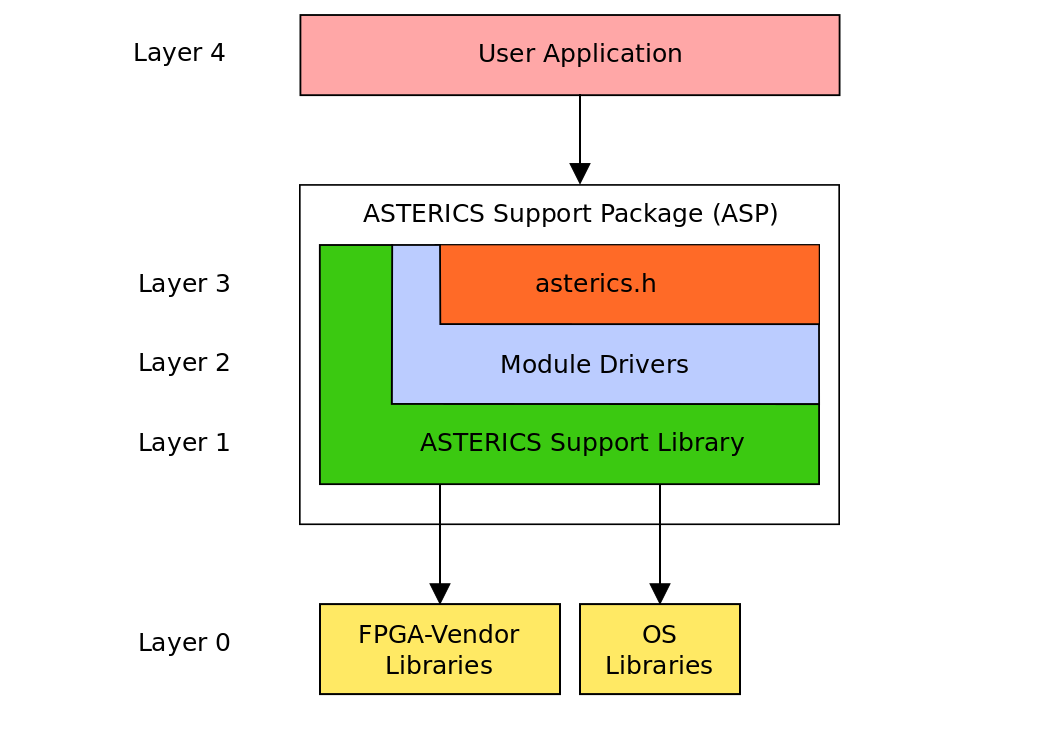
\includegraphics[width=0.8\linewidth,clip]{figs/software_stack.png}
    \caption{Overview of the \asterics software stack}
    \label{fig:software-stack}
\end{figure}



%%%%%%%%%%%%%%%%%%% 4.2. ASTERICS Support Library %%%%%%%%%%%%%%%%%%%%%%%%%%%%


\section{The \asterics Support Library (ASL)}

\secauthor{Alexander Zöllner, Gundolf Kiefer}


The \textit{\asterics Support Library} is the main interface between hardware and application software within the \asterics framework.
It contains all vendor and platform dependencies for performing the actual hardware accesses.
Towards software, the \textit{ASL} offers static register-based interfaces to the \asterics hardware modules of the hardware image processing chain and a number of utilities, such as for synchronization or memory allocation.
The \textit{ASL} uses the appropriate implementation for the corresponding functionality, depending on the environment parameter settings within \texttt{as\_config.h}.
Therefore, the \textit{ASL} has to be included across the \asterics software stack, whenever a piece of software indents to access the hardware or utilizing mechanics which are platform dependent.




%%%%%%%%%%%%%%%%%%% 4.3. ASTERICS Support Package %%%%%%%%%%%%%%%%%%%%%%%%%%%%


\section{Contents of an \asterics Support Package (ASP)}

\secauthor{Alexander Zöllner, Philip Manke, Gundolf Kiefer}

Table~\ref{table:asp-contents} shows the contents of an \textit{\asterics Support Package}, used for describing a specific hardware image processing chain and choosing the target environment of the \textit{ASP}.
If a given hardware image processing chain is to be utilized for several environments, a corresponding \textit{ASP} has to be provided for each one.
Although most contents of the \asterics software stack can be copied for multiple \textit{ASPs} and processing chains, some parts have to be replaced, since they depend on the actual hardware implementation and the environment.
The files \texttt{asterics.h} and \texttt{as\_config.mk} are the only ones which are affected.
The former has to be updated each time the underlying hardware image processing chain is altered in regards of its modules.
This mainly includes adding or removing hardware modules, changing their pre-synthesis parameters or their absolute start address.
Therefore, it is recommended to update the \textit{asterics.h} header file each time one of the parameters of the hardware image processing chain is touched.
On the other hand, the \texttt{as\_config.mk} file reflects the settings of the environment, on which the \textit{ASP} and hardware image processing chain is deployed.
Prominent parameters are the whether an operating system is utilized or the SoC vendor, who usually provides low level software drivers for interfacing the hardware.
Thus, it only needs to be replaced when the target environment changes (which usually occurs less frequent than changing the hardware implementation during development).
The remaining files of the \textit{ASP} are left untouched across multiple hardware image processing chains and environments.


\begin{longtable}[ht]{|l|l|l|}
    \hline
    \multicolumn{1}{|c|}{\textbf{File Name}} & \multicolumn{1}{c|}{\textbf{Includes}} & \multicolumn{1}{c|}{\textbf{Description}}\\
    \hline 
    \hline 
    \endhead
    
    asterics.h & \parbox{5cm}{\ \\
        as\_support.h\\
        as\_\texttt{<}\textit{module}\texttt{>}.h\\
    } &
    \parbox{7cm}{\ \\
        Library to be included by the user application software.\\
        Inlcudes all module driver headers and defines hardware addresses.\\
    }\\
    \hline
    as\_support.h & \parbox{5cm}{\ \\
        as\_config.h\\
        as\_kernel\_linux\_if.h(*)\\
    } &
    \parbox{7cm}{\ \\
        The \textit{\asterics Support Library} for vendor abstraction and interfacing the hardware.\\
        (*) Only included when compiled for Linux kernel or POSIX compliant operating systems.\\
    }\\
    \hline
    as\_support.c & \parbox{5cm}{\ \\
        as\_support.h\\
    } &
    \parbox{7cm}{\ \\
        Contains the function definitions for the \textit{\asterics Support Library}.\\
    }\\
    \hline
    as\_\texttt{<}$module$\texttt{>}.h & \parbox{5cm}{\ \\
        as\_support.h\\
    } &
    \parbox{7cm}{\ \\
        Provides macros and interface functions of the associated hardware module.\\
        $module$ is replaced by the actual name of the hardware module.\\
    }\\
    \hline
    as\_\texttt{<}module\texttt{>}.c & \parbox{5cm}{\ \\
        as\_\texttt{<}$module$\texttt{>}.h\\
    } &
    \parbox{7cm}{\ \\
        Implements the functionality of the module driver.\\
    }\\
    \hline
    as\_config.h &  &
    \parbox{7cm}{\ \\
        Contains macros for defining the environment the \textit{ASP} is built for.\\
        It is generated from as\_config.mk.\\
    }\\
    \hline
    as\_config.c &  &
    \parbox{7cm}{\ \\
        Contains an identification number and build date of config.h.\\
        It is generated from as\_config.mk or by \textit{Automatics}.\\
    }\\
    \hline
    as\_config.mk &  &
    \parbox{7cm}{\ \\
        Sets the platform and operating system configuration of the \textit{ASP}\\
        Makefile fragment.\\
    }\\
    \hline
    
    \caption{Contents of an \textit{\asterics Support Package (ASP)} for a specific \textit{\asterics chain}.}
    \label{table:asp-contents}
\end{longtable}




%%%%%%%%%%%%%%%%%%%%%%%%%%%%% 4.4. as_memio %%%%%%%%%%%%%%%%%%%%%%%%%%%%%%%%%%


%%%%%%%%%%%%%%%%%%%%%%%%%%%%%%%%%%%%%%%%%%%%%%%%%%%%%%%%%%%%%%%%%%%%%%%%%%%%%%
%%
%% This file is part of the ASTERICS Framework. 
%%
%% Copyright (C) Hochschule Augsburg, University of Applied Sciences
%% Efficient Embedded Systems Group
%%
%% Author(s): Gundolf Kiefer <gundolf.kiefer@hs-augsburg.de>
%%
%%%%%%%%%%%%%%%%%%%%%%%%%%%%%%%%%%%%%%%%%%%%%%%%%%%%%%%%%%%%%%%%%%%%%%%%%%%%%%



\section{Transferring Data between Hardware and Software}\label{ch:04-software-data-trans}

\secauthor{Alexander Zöllner, Gundolf Kiefer}

\subsection{Brief Description}

The main purpose of the \asterics framework is enhancing image processing tasks using codesigns of hardware and software.
This requires transferring data between both subsystems in a convenient and efficient manner.
For accomplishing this task, the memory modules of \asterics are used for performing the actual data transfer. 
Since setting up data transfers has to be managed by the software stack, respective methods are provided.
These methods vary in their complexity and required overhead expected from the user.
The appropriate method can be chosen depending on the requirements of the application.

\subsection{Manual Data Transfer Management}
This method is the most direct way for transferring data by interfacing the corresponding memory module, using their module driver (see Chapter~\ref{ch:07-basic-mods-in_out}).
Here, a sufficient physically concurrent memory area has to be provided to the corresponding memory module, which is referred to as \textit{buffer} for (intermediately) storing data.
The user is supposed to manage the contents of the \textit{buffer} manually, to prevent its under- or overflows as well as inadvertently overwriting data.
Further, the status of the memory module has to be read from its hardware registers in order to determine whether a data transfer has been finished (\textit{state/control} register) or which parts of the \textit{buffer} have already been processed (\textit{current hw addr} register).
The double buffering scheme of the memory modules for queuing data transfers may be used for utilizing more than one \textit{buffer}.

Managing the data transfers directly gives the user exclusive control, allowing to also implement customized data transfer strategies.
However, preventing data loss has to be taken care of explicitly.


\subsection{POSIX-like Data Transfer Management}
For transferring data in a more convenient manner, the \asterics framework offers POSIX-like interfaces to the user, which are part of the software module \texttt{as\_memio} (memory input/output).
This module includes implementations for \textit{open}, \textit{read}, \textit{write} and \textit{close}, respectively.
Instead of having the user manage the data transfers and organizing the \textit{buffer(s)} for the memory module manually, these tasks are carried out by \textit{as\_memio}.
The user has to simply call \textit{open}, where the actual memory module is referenced.
The \texttt{as\_memio} module handles the internal specifics required for setting up data transfers.
These can be requested by calling either \textit{write} for transferring data to the hardware, using an \texttt{as\_memreader} module, or \textit{read} for obtaining data from the hardware processing chain, using an \texttt{as\_memwriter}.
Here, an opaque structure is provided to \texttt{as\_memio} (which is obtained by \textit{open}), along with the desired amount of data and a \textit{user buffer}.
This \textit{user buffer} is used for providing the data to be transferred or receiving data from \texttt{as\_memio}.
Once the request from the user has been served, the actual number of transferred bytes are returned to the user, which may be equal or less than the requested number.
Further, the \textit{user} buffer contains the amount of data, which has been served by the \texttt{as\_memio} module for \textit{read} calls.
For \textit{write} calls, the \textit{user buffer} is left untouched and may be used immediately by the user again after the function returns.
The \texttt{as\_memio} module internally manages the data for either direction and interfaces the associated memory module accordingly for transferring the data.
Provided the hardware processing chain supports the \texttt{STALL} mechanic (see Chapter~\ref{ch:05-03-interfaces-as_stream}), the \texttt{as\_memio} module can guarantee that no data is lost.









%%%%%%%%%%%%%%%%%%%%%%%%%%%%% 4.5. Linux Driver %%%%%%%%%%%%%%%%%%%%%%%%%%%%%%


%%%%%%%%%%%%%%%%%%%%%%%%%%%%%%%%%%%%%%%%%%%%%%%%%%%%%%%%%%%%%%%%%%%%%%%%%%%%%%
%%
%% This file is part of the ASTERICS Framework. 
%%
%% Copyright (C) Hochschule Augsburg, University of Applied Sciences
%% Efficient Embedded Systems Group
%%
%% Author(s): Gundolf Kiefer <gundolf.kiefer@hs-augsburg.de>
%%
%%%%%%%%%%%%%%%%%%%%%%%%%%%%%%%%%%%%%%%%%%%%%%%%%%%%%%%%%%%%%%%%%%%%%%%%%%%%%%



\section{The Linux Kernel Driver} \label{ch:04-05-software-linux}

\secauthor{Alexander Zoellner}

\infobox{The Linux kernel driver is currently in development. The following text is in reference to an older version of the kernel driver - some information may be out of date.}

\subsection{Brief Description}

Within \asterics great emphasis is put on its usability for developing new image processing applications in a fast and convenient manner.
Utilizing an operating system is a common practice since it already provides a great deal of functionality, such as a network stack and memory management.
Further, required software is either already available or can be easily installed by using the package manager.
Being able to seamlessly integrate \asterics into own applications

As Linux is commonly used for embedded applications, the Linux character device driver \texttt{as\_driver} has been developed for \asterics.
This driver is able to operate with any \asterics-based image processing chain by providing a set of interfaces between hardware and software.
\asterics-chains can be exchanged on the FPGA without having to reload or recompile \texttt{as\_driver}.
The driver covers standard POSIX file operations, mapping memory regions to user as well as basic register-based hardware accesses.
The driver provides methods for altering the interfaces to hardware at runtime to cater to any \asterics-chain.


\subsection{Architecture}

Figure~\ref{fig:driver-architecture} shows the principle architecture of \texttt{as\_driver}.
It consists of the main parts \textit{device class}, \textit{device array}, \textit{file operation structures}, \textit{Init} and \textit{Exit}.
The latter two are methods which are the constructor and destructor of the kernel module, respectively.
They are called when the kernel module is loaded to the kernel or unloaded.
\textit{Init} performs the minimal required amount of initialization of the kernel module, such as registering it to the kernel and publishing its file operations.
For this reason, a \textit{device class} is created, which consists of a \textit{major number}, which refers to the kernel module itself and a number of \textit{minor numbers}.
Each \textit{minor number} is associated with a specific device of the kernel module, whereas the \textit{major number} indicates the responsible device driver for the device.
As shown in the figure, a number of \textit{minor numbers} are requested but not published immediately, indicated by \textit{empty} slots in the \textit{device class}.
The \asterics device driver organizes its devices in a \textit{device array} of a static size.
Devices may be added or removed from the \textit{device array}.
Slots which are not yet occupied by a device are indicated by \textit{uninitialized}.
Each device is associated with a \textit{minor number} and a \textit{file operation structure}.
The five \textit{file operation structures} are the actual device types available to \texttt{as\_driver}.
Each structure defines a set of \textit{methods}, which are used to overwrite the default file operation methods provided by the kernel.
This is accomplished by linking to one of these \textit{file operation structures} when initializing the device.
As shown by the \texttt{as\_memio} device, devices of the same type also point to the same \textit{file operations structure} and use its \textit{methods}.
The first device, namely the \texttt{as\_control} device, is created by \textit{Init} and the first \textit{minor number} is used.
Additional devices can be added or removed by using the \textit{methods} of the \texttt{as\_control} device, which publishes the device to the kernel by adding the associated \textit{minor number} to the \textit{device class} and linking to the appropriate \textit{file operation structure}.
\textit{Exit} on the other hand, deletes all allocated parts of the \asterics device driver and unregisters the kernel module and all its devices.
Resources obtained by the kernel module during its lifetime are released to the operating system again.

Up to this point, devices contained in the \textit{device array} are only known by the kernel but not yet accessible by the user application.
This requires to link the devices to the file system of the operating system in order to perform operations on the it.
A device can be published to the user space by creating a \textit{device node}, which is an entry point on the file system.
A \textit{device node} is associated with a certain device, by specifying its \textit{major} and \textit{minor number} upon creating the node.
As aforementioned, the \textit{major number} is used to tell the kernel which kernel module it should use when calling the file operations of the device.
The \textit{minor number} is used by the kernel module to identify the actual device to be accessed.
For creating the \textit{device node}, a path and a name on the file system has to be chosen where the node should appear.
When working with Linux, the location \textit{/dev/} is usually used for devices.
Once the \textit{device node} has been created, it can be used for the path argument for the open file operation to access the device and subsequently perform additional actions by calling the appropriate file operations.
Since the \textit{device node} is only a link to a device, it can also be created before the actual device exists, provided that the \textit{major} and \textit{minor number}, which is going to be used, is already known at this point.
Trying to access the \textit{device node}, without the actual device existing, will fail for obvious reasons.
The node can be used as soon as the associated device has been published to the kernel.
Naturally, if the device is removed, the node will cease to perform any accesses to the device.

The structure of \texttt{as\_driver} allows to create additional devices at runtime and therefore can be used for any \asterics-based image processing chain implemented on hardware.
Moreover, devices can also be deleted at runtime, with the kernel module displaying similar behavior as if it has just been loaded to the kernel.
Therefore, the processing chain can also be replaced at runtime, by simply instructing the kernel module to delete all devices and subsequently creating new ones.

\begin{figure}[ht]
    \centering
    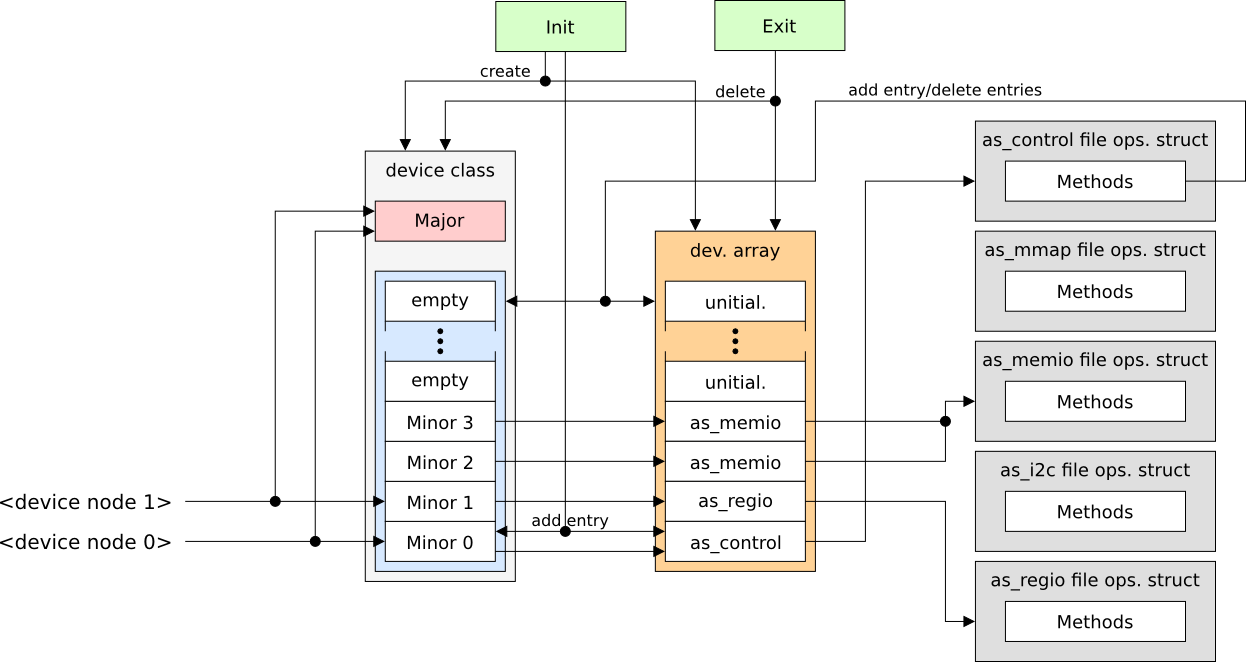
\includegraphics[width=0.8\linewidth,clip]{figs/driver_architecture.png}
    \caption{Architecture of the \asterics Linux kernel driver (\texttt{as\_driver})}
    \label{fig:driver-architecture}
\end{figure}

Table~\ref{table:device_driver:driver-files} lists the files of \texttt{as\_driver} and their meaning.
They can be found at "tools/as-linux/src/kernel\_module/asterics-driver".

\begin{longtable}[ht]{|l|c|l|l|}
    \hline
    \multicolumn{1}{|c|}{\textbf{Name}} & \multicolumn{1}{c|}{\textbf{Type}} & \multicolumn{1}{c|}{\textbf{Description}} \\
    \hline
    \texttt{as\_driver} & c source file & \parbox{7.5cm}{\ \\
        Implementation of the \asterics device driver.\\
    }\\
    \hline
    \texttt{as\_driver} & c header file & \parbox{7.5cm}{\ \\
        Compile time parameters and data structure of the \asterics device driver.\\
    }\\
    \hline
    \texttt{as\_linux\_kernel\_if} & c header file & \parbox{7.5cm}{\ \\
        Data structures and commands for \texttt{ioctl}/\texttt{unlocked\_ioctl} and device types used by the \texttt{as\_control} device. \\
    }\\
    \hline
    \texttt{as\_config} & c header file & \parbox{7.5cm}{\ \\
        Flags used for determining the features and environment the software has been compiled for. \\
        It is used for determining the appropriate implementation for functions provided by the \asterics software stack. \\
    }\\
    \hline
    \texttt{Makefile} & GNU makefile & \parbox{7.5cm}{\ \\
        Builds the kernel module.\\
    }\\
    \hline
    \caption{Files of the \asterics device driver}
    \label{table:device_driver:driver-files}
\end{longtable}


\subsection{Compile-Time Options}

The \texttt{as\_driver} offers a set of configuration parameters, which can be set at compile-time and therefore take effect, once the device driver is loaded.
Table~\ref{table:device_driver:config} lists the available parameters.
The device driver manages its devices in a list, with a fixed number of entries.
The parameter \texttt{NUM\_MAX\_DEVICES} is used to define the number of entries in the list, which correlates to the maximum number of devices which can be created by the \texttt{as\_control} device.
The number of devices has to be at least set to two, since one entry will be already occupied by the \texttt{as\_control} device.
As for the maximum number of entries, it is best to make use of the define found in the library \textit{kdev\_t.h}, which defines the maximum available amount of supported minor numbers for device drivers.
Each device requires a minor number in order for the kernel to distinguish between them.

The parameter \texttt{TIMER\_INTERVAL} is used to define the interval in jiffies for generating a timer interrupt.
The actual interval depends on the settings for \textit{HZ} of the platforms. 
For embedded platforms, it usually defaults to 100 Hz, which means the interval has a granularity of 10 ms.
Although the kernel provides an interface for converting a desired time in milliseconds to the appropriate number of jiffies, it cannot forgo the configured granularity of the interval.
This means, the resulting time may not match the actual requested time by the user, which could lead to confusion.
Thus, the parameter \texttt{TIMER\_INTERVAL} uses jiffies to clearly indicate its platform dependency.
An appropriate comment has also been added to the header file of the device driver to state this circumstance.
Depending on the expected amount of data to be transferred between software and hardware, this value can be increased or lowered accordingly.
For a low amount of data, the user may consider to increase the timer value, since calls to read or write of the \texttt{as\_memio} device may block for an extended period of time, until data becomes available again.
Since the interrupt is also used to wake up any sleeping processes, they might block immediately again, since no data has been become available between two consecutive interrupts.

\begin{longtable}[ht]{|l|c|c|l|}
    \hline
    \multicolumn{1}{|c|}{\textbf{Name}} & \multicolumn{1}{c|}{\textbf{Type}} & \multicolumn{1}{c|}{\textbf{Range}} & \multicolumn{1}{c|}{\textbf{Description}} \\
    \hline
    \texttt{NUM\_MAX\_DEVICES} & unsigned & 2 - MINORMASK & \parbox{5.5cm}{\ \\
        Maximum number of devices available to the driver \\
    }\\
    \hline
    \texttt{TIMER\_INTERVAL} & unsigned & 1 - 4294967295 & \parbox{5.5cm}{\ \\
        Timer interval in jiffies \\
    }\\
    \hline
    \caption{Configuration options for the ASTERICS device driver}
    \label{table:device_driver:config}
\end{longtable}


\subsection{Register-based IO Device}

In order to access the physical addresses of the hardware registers, they have to be mapped to a virtual kernel address area first.
Listing~\ref{code:regio-mapping} shows the functions, which have to be called for being able to access the physical address region.
The first function, \texttt{request\_mem\_region} is used to reserve a named address region from the kernel. 
By calling this function the driver tells the kernel, that it is going to use this address region.
No actual mapping is performed at this point, only a reservation request.
This prevents other drivers from mapping the same address region and thus competing accesses.
The first parameter \texttt{start} specifies the physical address, where the requested region starts, with a size of \texttt{n} bytes.
The last parameter \texttt{name} provides a pointer to a string, containing the name of the region.
If the request has failed, a NULL value is returned by these function, otherwise a non-NULL value.

The function \texttt{ioremap} is used to perform the actual mapping of the memory region.
It also requires the physical start address \texttt{start} of the region as well as its \texttt{size} in bytes.
The return value is a virtual kernel address, which can be used to perform the actual accesses to hardware.

The mapping of the memory region is performed by the \texttt{as\_control} device upon creating the \texttt{as\_regio} device.
Similarly, unmapping and releasing the memory region is either performed by the \texttt{as\_control} device or at the point \texttt{as\_driver} is unloaded.

\begin{lstlisting}[style=CStyle, label=code:regio-mapping, caption=Functions for allowing to access physical addresses]
struct resource * request_mem_region (
		unsigned long start, unsigned long n, const char *name)

void * 	ioremap (unsigned long phys_addr, unsigned long size)

\end{lstlisting}

The following Listing~\ref{code:regio-access} shows the functions used by the \texttt{as\_regio} device of the \asterics device driver for accessing the hardware registers of the hardware.
For obtaining the currently stored data in the hardware register, \texttt{ioread32} is used.
As the name suggests, it is used to read the value from the register at \texttt{addr}, which is the virtual kernel address, previously mapped by calling the aforementioned functions.
The return value is the current register content.
For writing data to the register, \texttt{iowrite} is used, which takes two parameters, the value to be written (\texttt{val}) and the virtual kernel address \texttt{addr}.
It is worth to note, that the currently used platforms, on which the device driver is used, are exclusively 32 bit systems and the hardware registers have also a size of 32 bits.

\begin{lstlisting}[style=CStyle, label=code:regio-access, caption=Functions for accessing hardware registers]
unsigned int ioread32(void __iomem *addr)

void iowrite32(u32 val, void __iomem *addr)

\end{lstlisting}

The \texttt{as\_regio} device provides only an implementation for the \textit{unlocked\_ioctl} method, whereas for open and close the default implementations provided by the kernel are used.
Similar to the \texttt{as\_control} device (Chapter TBD), the \texttt{cmd} parameter is used to inform the device, whether the method has been called by user or kernel space, in order to copy the data of \texttt{arg} appropriately.
The \texttt{unlocked\_ioctl} method can also be called by kernel space, since other devices of the \asterics device driver are also required to configure the hardware.
Instead of performing accesses to the hardware registers on their own, they make use of the \texttt{as\_regio} device.
The \texttt{arg} parameter of \texttt{unlocked\_ioctl} is a pointer to a \texttt{as\_ioctl\_params\_t} structure, which is part of \texttt{as\_linux\_kernel\_if.h}.
The \texttt{cmd} parameter of this structure can either be \texttt{AS\_IOCTL\_CMD\_READ} or \texttt{AS\_IOCTL\_CMD\_WRITE}.
In order to access the register correctly, the field \texttt{address} has to hold the physical address of the register.
This address may be obtained by the tools used for implementing the hardware design (e.g. Vivado).
For write accesses, the parameter \texttt{value} is written to the register, whereas for read accesses, the value of the register is directly returned by \textit{unlocked\_ioctl}, instead of copying it to the field of the structure.
The \texttt{user\_addr\_start} is not used by the \texttt{as\_regio} device and the user may decide to not explicitly assigning a value to it.

The user calls the associated \textit{ioctl} method with the same parameters.


\subsection{I2C Device}

The \textit{i2c device} works identically to the \texttt{as\_regio} device and uses the same kernel mechanisms for obtaining a memory region and accessing the hardware registers.
A separate device has been added to the \asterics device driver, to be able to map the hardware addresses of the used hardware registers to a different address region, which is not adjacent to the one used for the \texttt{as\_regio} device.
The actual functionality for the I2C uses the \texttt{as\_i2c} module driver, which utilizes the device driver for performing accesses to its hardware registers.


\subsection{Memory IO Device}

The \texttt{as\_memio} device utilizes the \texttt{as\_memio} module driver for conveniently transferring data between application software and FPGA.
For being able to transfer data, the \texttt{as\_memio} device has to be associated with a memory module, which in turn is forwarded to the \texttt{as\_memio} module driver.
In order to use a specific \texttt{as\_memio} device right away, this task is carried out upon creating the device with the \texttt{as\_control} device.
Here, the \textit{base address}, \textit{memory bus interface width} and \textit{direction} has to be provided.
The \textit{base address} is the address of the first hardware register used by the corresponding memory module, which is required for configuring the module correctly.
This address can usually be obtained by the tool used for implementing the processing chain on the FPGA (e.g. Vivado by Xilinx).

Similarly, the \textit{interface width} is needed for aligning the data correctly for its transfers. 
The memory modules are synthesized for a certain bit width, which is also used for its port towards other hardware modules.
For this reason, \emph{byte enables} are currently not supported, which results in having to transfer a multiple of the \textit{interface width} of bytes.

Since the \textit{direction} of the data flow is determined by either using an \texttt{as\_memreader} (to FPGA) or a an \texttt{as\_memwriter} (from FPGA) module, it has also to be provided to the \texttt{as\_memio} device.
Although the \texttt{as\_memio} module driver supports both directions, only one can be used at a time, since an instance of the driver only manages one memory module at a time.

The file operation structure for the \texttt{as\_memio} device provides implementations for five methods, namely \texttt{open}, \texttt{read}, \texttt{write}, \texttt{unlocked\_ioctl} and \texttt{close}.
Principally, the \texttt{open} method performs a number of checks and sets up the \texttt{as\_memio} module driver for the specific memory module.

In a first step, the \textit{device array} is iterated to find the \texttt{device\_data\_t} structure (part of \texttt{as\_driver.h}), which represents the requested \texttt{as\_memio} device. 
Multiple instances of the \texttt{as\_memio} module driver using the same memory module conflict with each other, due to relying on status information of the module regarding the current data transfer.
Therefore, only one instance of a given \texttt{as\_memio} device is allowed.
This is guaranteed by using the variable \texttt{busy} of the \texttt{device\_data\_t} structure, which is of type \textit{atomic\_t}.
Since the access to the variable is atomic, only one process can successfully acquire the \texttt{as\_memio} device.

After having acquired the corresponding \texttt{as\_memio} device, the directions \texttt{flags} provided upon \texttt{open} are compared to the one set at the point the device has been created.
In this way, the user is informed if the wrong device has been accidentally requested, e.g. data is to be transferred from memory to the FPGA but the device only supports inverse direction.
If this has been the case, the \texttt{as\_memio} device is released again and provides an error message to the user, pointing out this mismatch.

Otherwise, \texttt{as\_memio\_open} of the \texttt{as\_memio} module driver is called with a set of configuration parameters.
Except for the \textit{interface width}, the default settings defined in the header file of the \texttt{as\_memio} module driver are used.
The allocation of the \textit{Ring Buffer} and the \textit{Buffer Handler} is carried out by the module driver internally, without requiring the device driver to explicitly allocate structures on its own.
The module driver returns a pointer to the \texttt{struct as\_memio\_file\_s} structure, which is used by the module driver for managing the memory module.
The pointer is assigned to the \texttt{memio\_file} field of the \texttt{device\_data\_t} structure of the device.

As the \texttt{as\_memio} device supports blocking and nonblocking data transfers, the presence of the \texttt{O\_NONBLOCK} flag is checked.
If this flag has not been provided upon calling \texttt{open}, a \textit{wait queue} is set up for the device, allowing it to sleep if the request number of bytes cannot be served right away.
Lastly, the variable \texttt{memio\_active} is set to inform the interrupt logic to serve this device.
Figure~\ref{fig:memio-open} summarizes the steps performed by the \textit{open} file operation method.

\begin{figure}[ht]
    \centering
    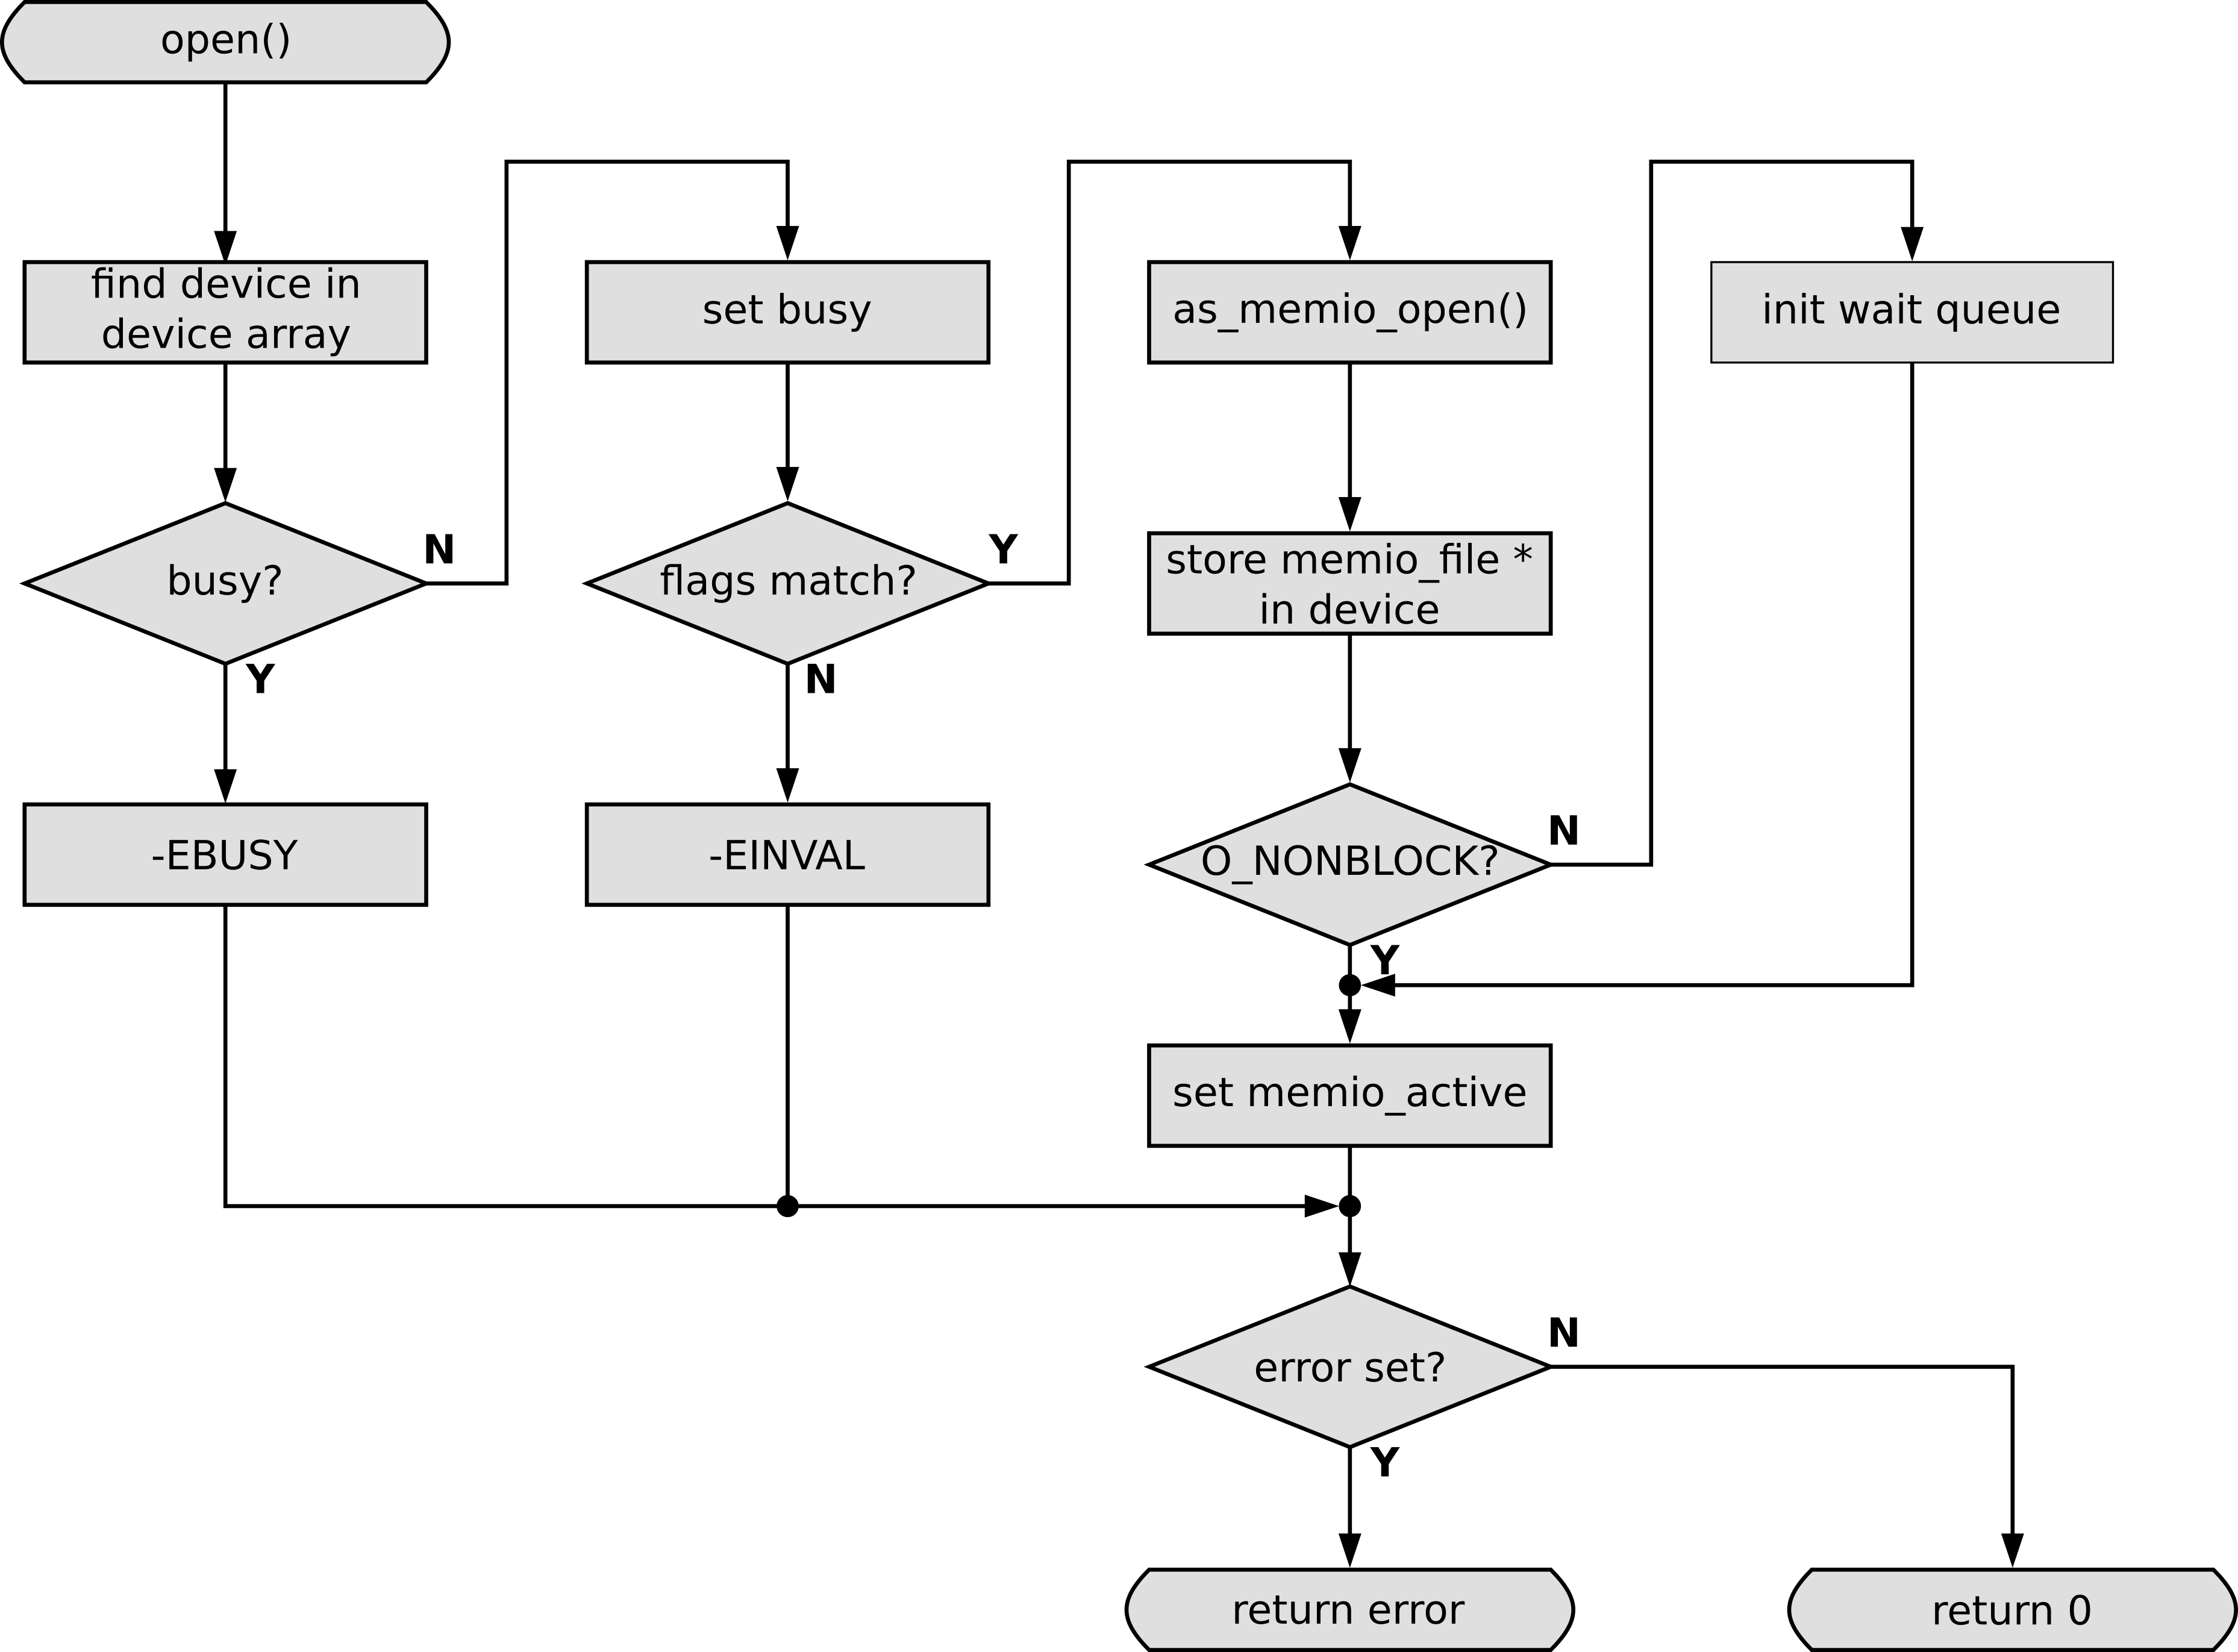
\includegraphics[width=0.7\textwidth,height=0.7\textheight,keepaspectratio]{figs/memio_open.png}
    \caption{Processing steps performed by the \texttt{open} method of the \texttt{as\_memio} device.}
    \label{fig:memio-open}
\end{figure}

For actually transferring data between main memory and the FPGA, the methods \texttt{read} and \texttt{write} are used.
In order to prevent race conditions of multiple processes trying to read or write data at a given time, using the same \texttt{as\_memio} device, a \textit{mutex} is used.
For this purpose, the \texttt{device\_data\_t} structure of the device provides the variable \texttt{access\_lock}.
Similar to \texttt{open}, the provided direction flag is evaluated, since only either of the two file operations is supported, depending whether a \texttt{as\_memreader} or \texttt{as\_memwriter} module is associated.
If the requested file operation is not supported by the specific \texttt{as\_memio} device, an error message points out the mismatch and a negative value is returned.
For this reason, the user has to evaluate the return value of the used function, at least for the first call.

Subsequently, the presence of \texttt{O\_NONBLOCK} is checked.
If the flag has been provided, the specified number of bytes and the \textit{User Buffer} is passed to the \texttt{as\_memio\_[read/write]} function of the \texttt{as\_memio} module driver.
The \textit{Buffer Handler} tries to serve the request as far as possible by transferring data between the \textit{User Buffer} and the \textit{Ring Buffer} and configuring the associated memory module accordingly.
Since the data cannot be directly copied between user and kernel space, the function  \textit{copy\_[to/from]\_user} has to be used.
Therefore, the module driver checks whether it has been compiled for the Linux kernel or for a bare-metal application, using the setting provided by \texttt{as\_config.h}.
The actually transferred number of bytes is returned to the \texttt{as\_memio} device, which is equal or less than the requested number of bytes.
This number is then passed to the user, returning immediately without blocking even if the requested number has not been met.
The POSIX standard states, that a negative return value shall be passed to the user, in case no data has been transferred at all and the device would block with the \texttt{O\_NONBLOCK} flag being set.
However, since the \texttt{as\_memio} device does not block under any circumstance if the \texttt{O\_NONBLOCK} flag has been provided, no error code is returned in this case.
The \texttt{read/write} functions simply returns with a "0" for the number of bytes, which have been transferred.
The caller of the corresponding function is expected to evaluate the return value and call the function again, if the requested amount has not been served entirely.

If the \texttt{O\_NONBLOCK} flag is absent, the \texttt{as\_memio} device performs the same call to the \texttt{as\_memio} module driver.
If the module driver has been able to perform the data transfer completely, the method behaves in the same manner as if the flag had been provided.
However, in case the transferred number of bytes is less than specified, the \texttt{as\_memio} device sets up the condition variable \texttt{wake\_up\_cond} and sets the flag \texttt{register\_intr} before blocking by calling the function \texttt{wait\_event\_interruptible}.
The processor stops executing the blocking process.
When the interrupt handler wakes up the process again by setting the condition variable appropriately and calling the function \texttt{wake\_up\_interruptible}, the device driver calls \texttt{as\_memio\_[read/write]} function again with the remaining bytes to be transferred.
If the request has been served entirely, the file operation method of the \texttt{as\_memio} device exits.
Otherwise, the above mentioned procedure is repeated.
When exiting, the mutex is released again.
Figure~\ref{fig:memio-transfer} summarizes the processing steps performed by the \texttt{read} and \texttt{write} method of the \texttt{as\_memio} device.

\begin{figure}[ht]
    \centering
    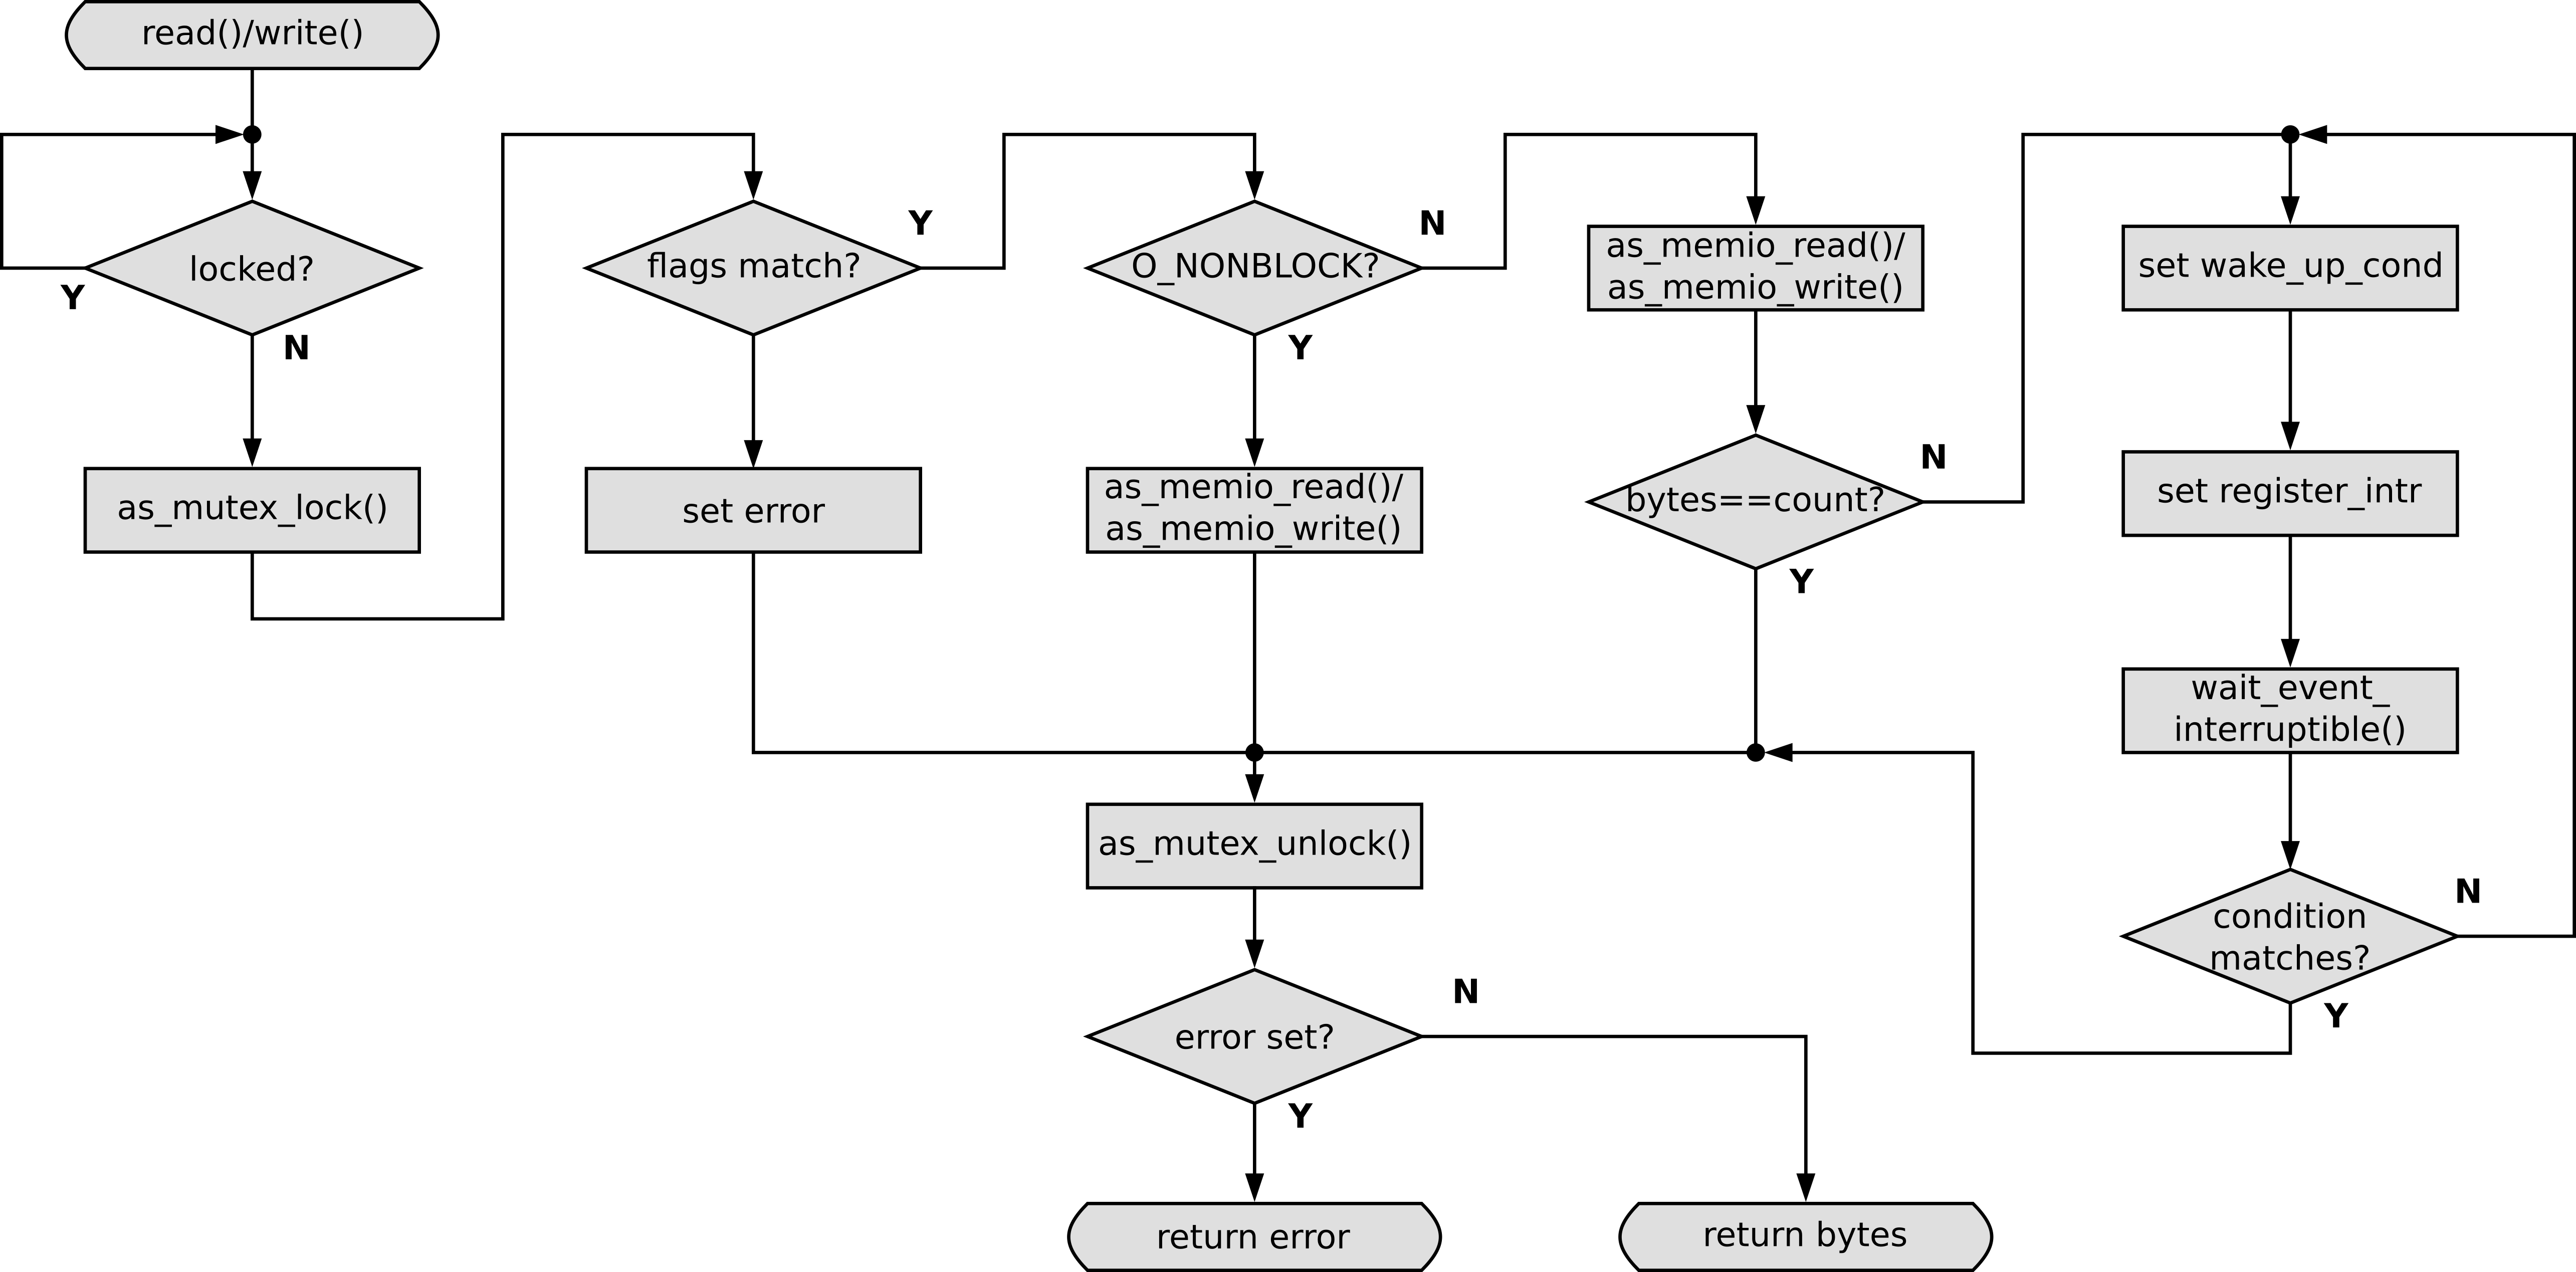
\includegraphics[width=\textwidth,height=\textheight,keepaspectratio]{figs/memio_transfer.png}
    \caption{Processing steps performed by the \textit{read} and \textit{write} method of the \texttt{as\_memio} device.}
    \label{fig:memio-transfer}
\end{figure}

The \texttt{unlocked\_control} method of the \texttt{as\_memio} device is used to trigger the \textit{Buffer Handler} of the \texttt{as\_memio} module driver to check whether there is data within its \textit{Ring Buffer} to be transferred.
The \texttt{as\_memio\_hw\_update} function of the module driver is used, by providing the pointer to the \texttt{memio\_file}.
Although this function is called by the module driver for every read and write request, it may occur that two calls to this function are required for transferring all data.
This is caused by the discrepancy of the differing access types of the \textit{Buffer Handler} and memory module to the \textit{Ring Buffer}.
The former writes or reads circularly to or from the \textit{Ring Buffer}, i.e. if the upper boundary is reached, it continuous at the lower boundary automatically.
The memory module, however, can only perform data transfers on physically concurrent memory addresses.
If a wrap around is required, the \textit{section} of the memory module has to be configured up to the upper boundary of the \textit{Ring Buffer} and the second one starting at the lower boundary again.
Usually, an explicit call to the \texttt{unlocked\_ioctl} method is not required, since the interrupt handler of the \asterics device driver regularly calls \texttt{as\_memio\_hw\_update} for its \texttt{as\_memio} devices, which are currently being used (see Chapter~\ref{device_driver:interrupts}).\newline

The \texttt{close} method of the \texttt{as\_memio} device resets the two variables, which are used for the interrupt logic of the device driver, \texttt{memio\_active} and \texttt{register\_intr}. 
In order to return the acquired resources by the \texttt{as\_memio} module driver back to the kernel, it calls the function \texttt{as\_memio\_close}.
Additionally, the module driver performs a reset on the associated memory module.
This terminates all ongoing data transfers, since the allocated \textit{Ring Buffer} is deleted and thus the memory area is no longer valid.
The \texttt{as\_memwriter} assumes a passive behavior, which prevents it from blocking any associated hardware processing chain.


\subsection{Memory Mapped IO Device}

The \texttt{as\_mmap} device circumvents having to copy data on memory by utilizing a dedicated memory area, which is published to the user. 
This memory can be shared between hardware and software.
Since the Linux operating system utilizes virtual address spaces, actual physical memory cannot be accessed from user space in the same way as its virtual addresses.
However, this limitation can be lifted to some degree, by utilizing mechanisms provided by the kernel to publish certain areas of physical memory to the user.
This is accomplished by implementing the file operation method \texttt{mmap} in a device driver for mapping a physically concurrent area of memory into the virtual address space of the user.
For this reason, the \texttt{as\_mmap} device has to provide a memory area which meets the requirements for being able to be mapped.
Regarding the lifetime of a device driver, the required memory can be acquired at several stages, such as at the time being loaded as kernel module, upon device creation or when the corresponding device is actually used.
Since \texttt{as\_driver} aims at being operable for any kind of image processing chain without having to reload the kernel module, the actual number of devices required by the user cannot be determined at the time it is being loaded to the kernel.
As the aforementioned memory areas are only utilized by devices of the \texttt{as\_mmap} type, a single memory area is allocated for each \texttt{as\_mmap} device upon creation, using the \texttt{as\_control} device.
The size of the memory area is configurable by providing the appropriate parameter to the \texttt{as\_control} device.
The memory area is acquired by using the kernel function \texttt{\_\_get\_free\_pages}, which allocates a physically concurrent amount of memory and returns the start address of it, i.e. a virtual kernel address.
This address is stored within the device to be used later on for the file operation methods.
As a side note, only sizes up to 4 MB have been used.
Allocations are to the power of two.
For preventing memory leaks, the memory has to be released when the corresponding device is no longer needed, i.e. when it is deleted.

As already stated, it would also be possible to allocate the memory when using a file operation method, such as \texttt{open}.
However, allocating memory can take quite some time, especially when trying to acquire larger areas of memory.
Additionally, it tends to get worse the longer the system runs, as memory gets fragmented.
Usually, when the user attempts to interacts with a certain device, the associated functionality is to be utilized immediately without further downtime.
For this reason, the memory allocation has been shifted to the point, where the device is created, i.e. the \texttt{as\_control} device.

Once \texttt{open} has been called on the device, the allocated memory region can be mapped using the file operation \texttt{mmap}.
For the \texttt{open} and \texttt{close} file operations, the default implementations provided by the kernel are used.
For actually mapping the allocated memory to the user space, the \texttt{vm\_end} and \texttt{vm\_start} field of the provided \textit{virtual memory aread (vma)} structure for \texttt{mmap} is used.
The difference between both is used for determining the number of bytes to be mapped.
If the number of bytes is equal or less than the one of the allocated area, the requested amount is mapped into the virtual address space of the user.
Listing~\ref{code:regio-mapping} lists the functions used for the actual mapping.
The first one, \texttt{virt\_to\_pfn}, is a macro for determining the \textit{page frame number (pfn)} of a given virtual address.
Since \texttt{\_\_get\_free\_pages} returns a virtual kernel address for the allocated memory area, this address is used.
The page frame number is required by the following function \texttt{remap\_pfn\_range}, which performs the actual mapping.
For the argument \texttt{virt\_addr}, the \texttt{vm\_start} field of the \texttt{vma} structure is used and for \texttt{size} the aforementioned difference of the \texttt{vm\_end} and \texttt{vm\_start} field.
Similar, the \texttt{vm\_page\_prot} field is used for the \texttt{prot} argument.
Usually, the user has to provide \texttt{PROT\_READ} and \texttt{PROT\_WRITE} when calling \texttt{mmap} from user space in order to be allowed to read and write to the mapped region.
The kernel provides the virtual address to user after the mapping, without requiring the developer of the device driver to perform any additional tasks.

\begin{lstlisting}[style=CStyle, label=code:regio-mapping, caption=Functions for allowing to access physical addresses]
#define virt_to_pfn(kaddr)

int remap_pfn_range(struct vm_area_struct *vma, unsigned long virt_addr,
				unsigned long pfn, unsigned long size, pgprot_t prot);

\end{lstlisting}

% unlocked\_ioctl
% - search mmap device
% - check if provided address is within mapped area 
Although the user can perform read and write accesses to the mapped memory area, transferring data to or from the hardware requires an explicit configuration of an appropriate memory module, depending on the desired direction.
This task is accomplished by using the file operation \texttt{ioctl} in user space, which results in calling the \texttt{unlocked\_ioctl} method of the \texttt{as\_mmap} device by the kernel.
For its \texttt{arg} parameter, the \texttt{as\_ioctl\_params\_t} structure is used.
The \texttt{cmd} field is used for determining the direction of the transfer, which can either be \texttt{AS\_IOCTL\_CMD\_READ} or \texttt{AS\_IOCTL\_CMD\_WRITE}.
The commands are defined in the interface header file \texttt{as\_linux\_kernel\_if.h} of the device driver.
The former requires a \texttt{as\_memwriter} module, whereas the latter requires a \texttt{as\_memreader} module.

The following parameter \texttt{address} specifies the base address of the memory module to be used for the data transfer.
Since the \texttt{as\_mmap} device is not bound to a specific memory module, an appropriate memory module has to be associated, which is either a \texttt{as\_memreader}, if the parameter \texttt{AS\_IOCTL\_CMD\_WRITE} has been provided, or a \texttt{as\_memwriter} for \texttt{AS\_IOCTL\_CMD\_READ}.
In order to find an appropriate memory module, the \textit{device array} is iterated to check if a \texttt{as\_memio} device exists, which is associated with the desired memory module.
This way, the \texttt{as\_mmap} device can use any of the defined memory modules within \texttt{as\_driver}.
If the memory module is defined within a \texttt{as\_memio} device, it checks the \texttt{busy} flag of the device, whether it is currently in use, i.e. the file operation \texttt{open} has been called on the requested \texttt{as\_memio} device.
By checking the flag, the device driver prevents interfering with any ongoing data transfers or the \textit{Buffer Handler}.
The flag is a variable of the type \textit{atomic\_t} which also helps to prevent possible race conditions for acquiring the shared resource, i.e. the memory module.

The \texttt{value} parameter is used to specify the number of bytes to be transferred between hardware and software.
Here, the device driver checks whether the requested amount can be transferred with the memory bus interface width used by the memory module.
The number of bytes has to be a multiple of the interface width.
Otherwise, a message is printed by the device driver to indicate the mismatch.

Lastly, the parameter \texttt{user\_addr\_start} is used to choose the start address within the memory mapped area, where the data transfer is supposed to begin.
The address is desired starting point within the virtual address space mapped to the user and is translated into the associated physical memory address.
Figure~\ref{fig:ioctl_mapping} illustrates the combination of the \texttt{user\_addr\_start} and \texttt{value} parameter for determining the memory area to be used for the data transfer.
The sum of both parameters must not exceed the boundaries of the memory area, as the device driver will perform any data transfer.

\begin{figure}[ht]
    \centering
    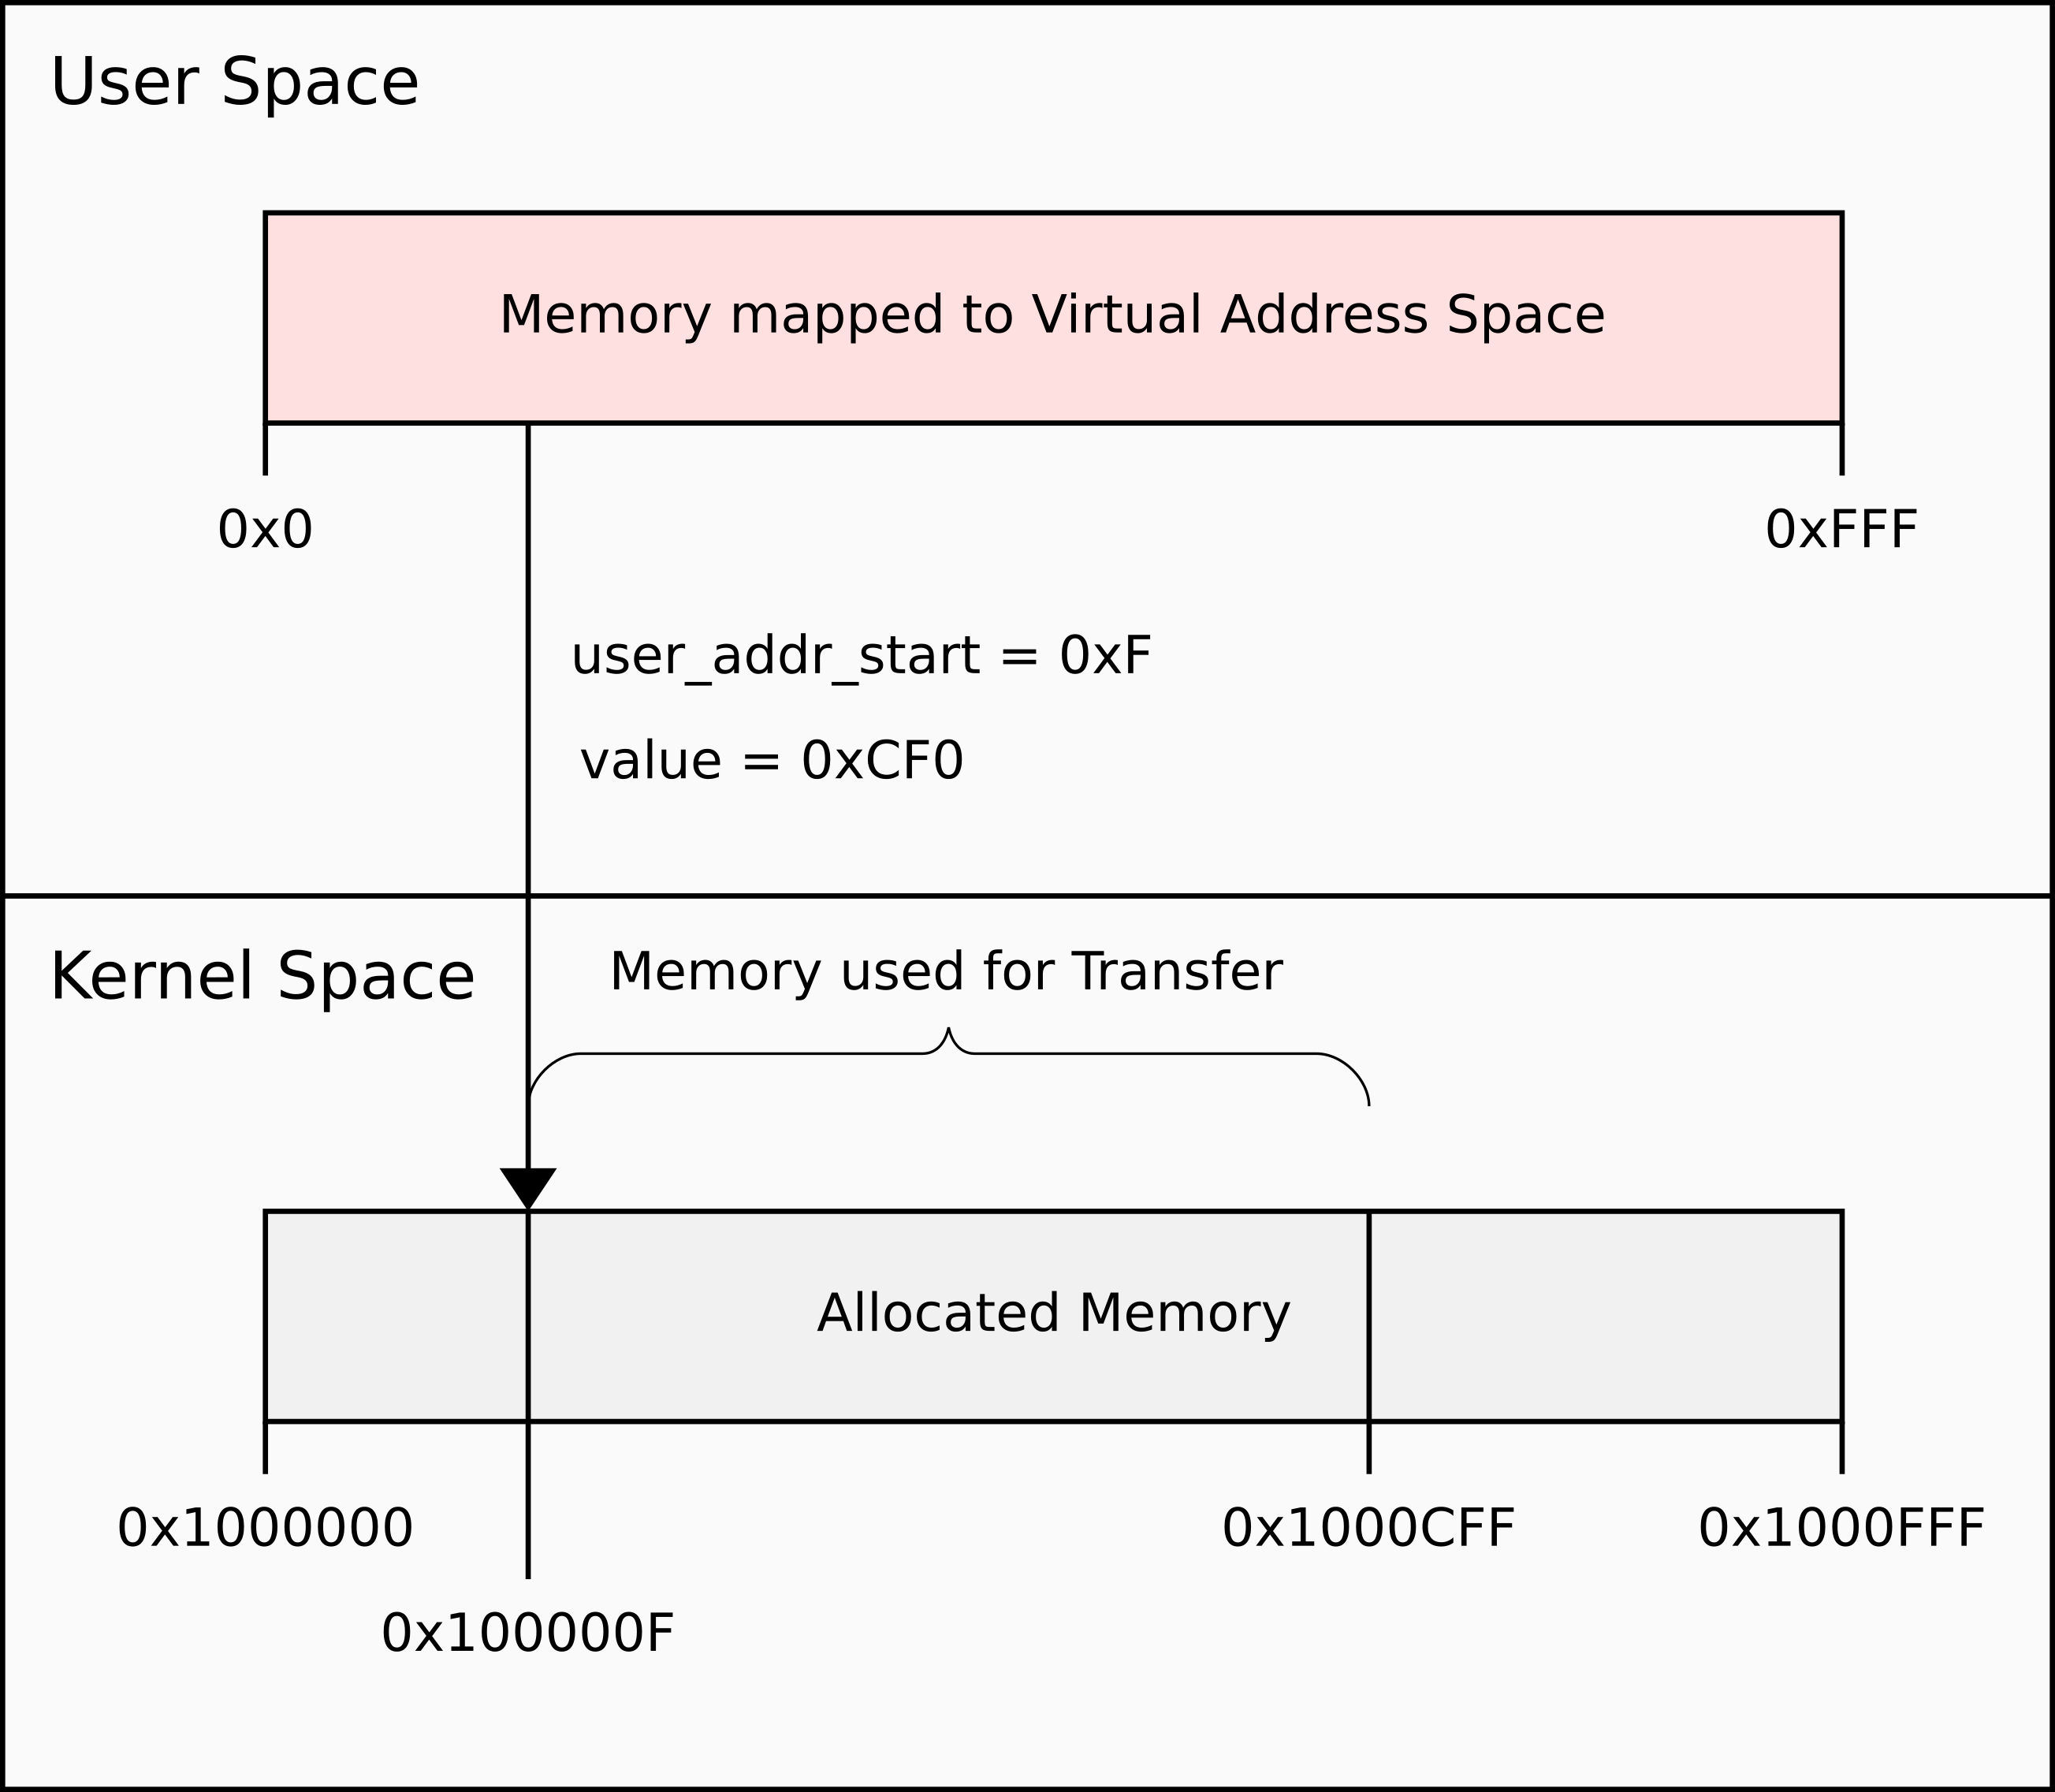
\includegraphics[width=0.5\textwidth,height=0.5\textheight,keepaspectratio]{figs/ioctl_mmap.png}
    \caption{Determining memory area for data transfer.}
    \label{fig:ioctl_mapping}
\end{figure}

After successfully determining the physical address area for the data transfer and acquiring the corresponding memory module, the device driver configures the memory module accordingly.
This is task is accomplished by using the interface functions of the \texttt{as\_reader\_writer} driver, which, in turn, uses the \texttt{as\_regio} device for accessing the hardware registers.
Thereby, the \textit{size} and the \textit{start address} of the \textit{section} is written to the hardware register.
For the remaining parameters, the default values specified in the \texttt{as\_reader\_writer} module driver are used.
As of the \texttt{as\_memwriter}, the \texttt{enable} and \texttt{disable\_on\_no\_go} flags are set.
This prevents the \texttt{as\_memwriter} to store any additional data in its \textit{Fifo Buffer} and thus negatively impacting other parts of the processing chain.
Subsequently, regardless of the memory module being used, the \texttt{go} flag is set to start the operation of the module.

Since the memory module is occupied with a data transfer at this point, it cannot be released by the \texttt{unlocked\_ioctl} method immediately, as the \texttt{as\_memio} device performs a reset on the memory module upon \texttt{open}.
This would terminate the current data transfer and thus has to be prevented.
Therefore, the status flag \texttt{done} is checked for determining whether the memory module has already finished its operation.
Depending on the image processing chain, this may take quite some time, which makes having to actively wait on the operation to finish undesirable.
For this reason, the \texttt{as\_memio} device utilizes a \textit{wait queue}, which is initialized upon creating the \texttt{as\_memio} device.
After checking the \texttt{done} flag, the process executing the \texttt{unlocked\_ioctl} method blocks by calling \texttt{wake\_event\_interruptible}.
If the process is woken up by the \textit{interrupt handler}, it checks the flag again.
In case the flag is still not set, the procedure is repeated.
Otherwise, the \texttt{busy} flag of the utilized \texttt{as\_mmap} device is unset, thus releasing the memory module.
Due to the aforementioned reason, the \texttt{as\_mmap} device currently does not support the \texttt{O\_NONBLOCK} flag.


\subsection{Control Device}

The \texttt{as\_control} device is used for creating and deleting additional devices at runtime.
It is the only device, which is created upon loading the device driver to the kernel and is always associated with the first \textit{minor number}, i.e. "0".
Similarly, it is the device with the first index within the \textit{device array}.
Since it is only used for managing the other devices of the driver, it only utilizes the mutex \texttt{access\_lock} of its associated \texttt{device\_data\_t} structure, which is also initialized upon loading the device driver.
For obvious reasons, \texttt{as\_control} device cannot delete itself or add additional instances of this device type to the device driver.

The functionality of the \texttt{as\_control} device is covered by the file operation method \texttt{unlocked\_ioctl}, which is the only method within its file operation structure.
As for all devices, \texttt{open} has to be called first, before being able to utilize it, however, no implementation is provided for neither \texttt{open} nor \texttt{close}.
This results in using the default methods provided by the kernel.

The mutex \texttt{access\_lock} is utilized to tackle potential race conditions.
Therefore, it always locks its mutex first, when executing its \texttt{unlocked\_ioctl} method.
Since the \texttt{as\_control} device is the only one being available after having loaded the \asterics device driver, adding further devices is the first task performed by the device and is therefore covered first.
In addition to the pointer to the structure representing the device (filp), \texttt{unlocked\_ioctl} method requires two parameters, namely \texttt{cmd} and \texttt{arg}.
The first parameter is used tell the \textit{as\_control} device whether the call to its method stems from the user or kernel space.
This is represented by providing either \texttt{CALLED\_FROM\_USER} or \texttt{CALLED\_FROM\_KERNEL}, respectively.
Both defines are part of the header file \texttt{as\_linux\_kernel\_if.h}, which is part of the \asterics device driver, but is also included for the application software.
Depending on the origin of the call, the \texttt{arg} parameter has to be handled differently.
For calls from kernel space, the data fields of the parameter can be accessed directly using common assignments.
However, if the call originates from user space, the function \texttt{copy\_from\_user} has to be used for copying the data fields of \texttt{arg} into a local structure of the same type, in order to be able to access them.
Generally, the request for creating or deleting devices is performed from user space, since the applications software determines the required devices for operating with the hardware residing on the FPGA.
Nonetheless, the access from kernel space is also supported, in case a different device driver is used for requesting additional devices.
As of the current state, this is mainly for future developments and applications of \texttt{as\_driver}.

The \texttt{arg} parameter, as already suggested, contains the information required by the \texttt{as\_control} device for creating devices.
In order to retrieve the information in a more convenient manner, a structure is used, which posses a number of fields.
This structure is of the type \texttt{as\_ctrl\_params\_t}, which is part of \texttt{as\_linux\_kernel\_if.h}.

The first field of this structure indicates, whether a new device has to be created, by providing \texttt{CMD\_CREATE\_DEVICE} for it.
If this parameter has been provided, the \texttt{as\_control} device checks, whether there are remaining entries in the \textit{device array} for adding an additional device.
This is done by comparing the global variable \texttt{initialized\_devices}, used for tracking the number of currently present devices, with \texttt{MAX\_DEVICES}, defining the maximal number of supported devices.
Each time a new device is added to the device driver, this variable is incremented.
Conveniently, this can also be used for index within the \textit{device array} for inserting the next device.
If the maximal number of devices has been reached, the \texttt{as\_control} device exits with an error message and return value, pointing out this circumstance.
Otherwise, the structure of the current device is initialized with default values, which mainly consists of setting pointers to NULL.
In the next step, the type of the requested device is determined by evaluating the parameter \texttt{dev\_type} of the \texttt{arg} parameter.
The type has to be one of the supported ones, which are also defined in \texttt{as\_linux\_kernel\_if.h}.
Currently supported devices are the \texttt{as\_regio}, \texttt{as\_i2c}, \texttt{as\_memio} and \texttt{as\_mmap} device.
The appropriate file operation structure is assigned to the \texttt{fops} field of the device structure.
The \texttt{interface\_width} and \texttt{flags}, for specifying the memory bus interface and supported direction for data transfer,  are assigned to fields with the same name of the device structure, respectively.
Subsequently, the \texttt{address\_range\_size} size field is assigned with the field with the same name.
The device is then created by using \texttt{cdev\_init} with the appropriate file operation structure.

For the \texttt{as\_regio} and \texttt{as\_i2c} device, a named memory region is requested.
The fields \texttt{dev\_address} and \texttt{address\_range\_size} of the \texttt{arg} parameter are used for specifying the physical start address and the size of the mapped region.
The address of the mapped region is assigned to the \texttt{baseaddress\_virt} field of the device structure.
The offset between the physical and virtual address is stored in the field \texttt{offset}.
Since the memory region has to have a name, \texttt{as\_iic} and \texttt{as\_regio} are used for the devices, respectively. 
However, as the names for the regions are unique, the device driver currently only supports one instance for each of the two device types.

For \texttt{as\_memio} devices, only the field \texttt{dev\_address} of the \texttt{arg} parameter is assigned to the field  \texttt{hw\_module\_addr}, to associate the memory module.
No further resources have to be allocated, since it is handled in its entirety within the file operation methods of the device.
Since the device is the only one associated with a specific hardware module, the aforementioned field is only used for this device.

Regarding the \texttt{as\_mmap} device, a new \texttt{mmap\_info\_t} structure is allocated for storing the \texttt{address\_range\_size} and the allocated physically concurrent memory, using \textit{\_\_get\_free\_pages}.
The size is used for determining the one for the memory allocation.
The start address of the allocated structure is assigned to the \texttt{mmap} field of the device structure.
Lastly, the \textit{wait queue} \texttt{wait} is initialized for allowing the device to block later on.

After the successful initialization of the device, it is published to the kernel by using \texttt{cdev\_add}.
For the \textit{minor number}, the current value of \texttt{initialized\_devices} is added to the first number, which has been used by the device driver.
In this case, the first \textit{minor number} is 0.
Lastly, the \texttt{initialized\_devices} variable is incremented and the mutex is unlocked again.


In order to prevent having to reload the kernel module of the \asterics device driver for removing devices, the \texttt{CMD\_REMOVE\_DEVICE} has been introduced to the \texttt{as\_control} device.
Since an array of a static size is used for managing the devices, deleting single devices would result in holes within the array, which would require a specific handling to avoid trying to access non-existing devices.
Alternatively, an array with a generic size could be used, where the size is increased or decreased each time a new device is created or deleted, respectively.
This approach would necessitate to allocate and reallocate major parts of the device representation at runtime.
As resources may grow scarce the longer the operation system runs, trying to create new devices are more likely to fail.
Usually, devices are deleted and replaced when the hardware processing chain is replaced.
Often times, the majority of the devices are affected, which is the main reason for having the \texttt{as\_control} device delete all other devices at once.
This is accomplished by looping the \textit{device array} and releasing all previously acquired resources.
The variable \texttt{initialized\_devices} is used as the upper boundary of the loop, since it represents the number of devices, which are currently used.
After the \texttt{as\_control} device has finished its task, \texttt{initialized\_devices} is set to 1 again, as only one device is present at this time, i.e. the \texttt{as\_control} device itself.

When deleting devices, care has to be taken, that none of these devices is currently used to prevent undesired behavior.
For this reason, it is recommended to call \texttt{close} on all devices except the \texttt{as\_control} device.


Figure~\ref{fig:control-dev} summarizes the essential functionality and the required steps of the \texttt{as\_control} device.

\begin{figure}[ht]
    \centering
    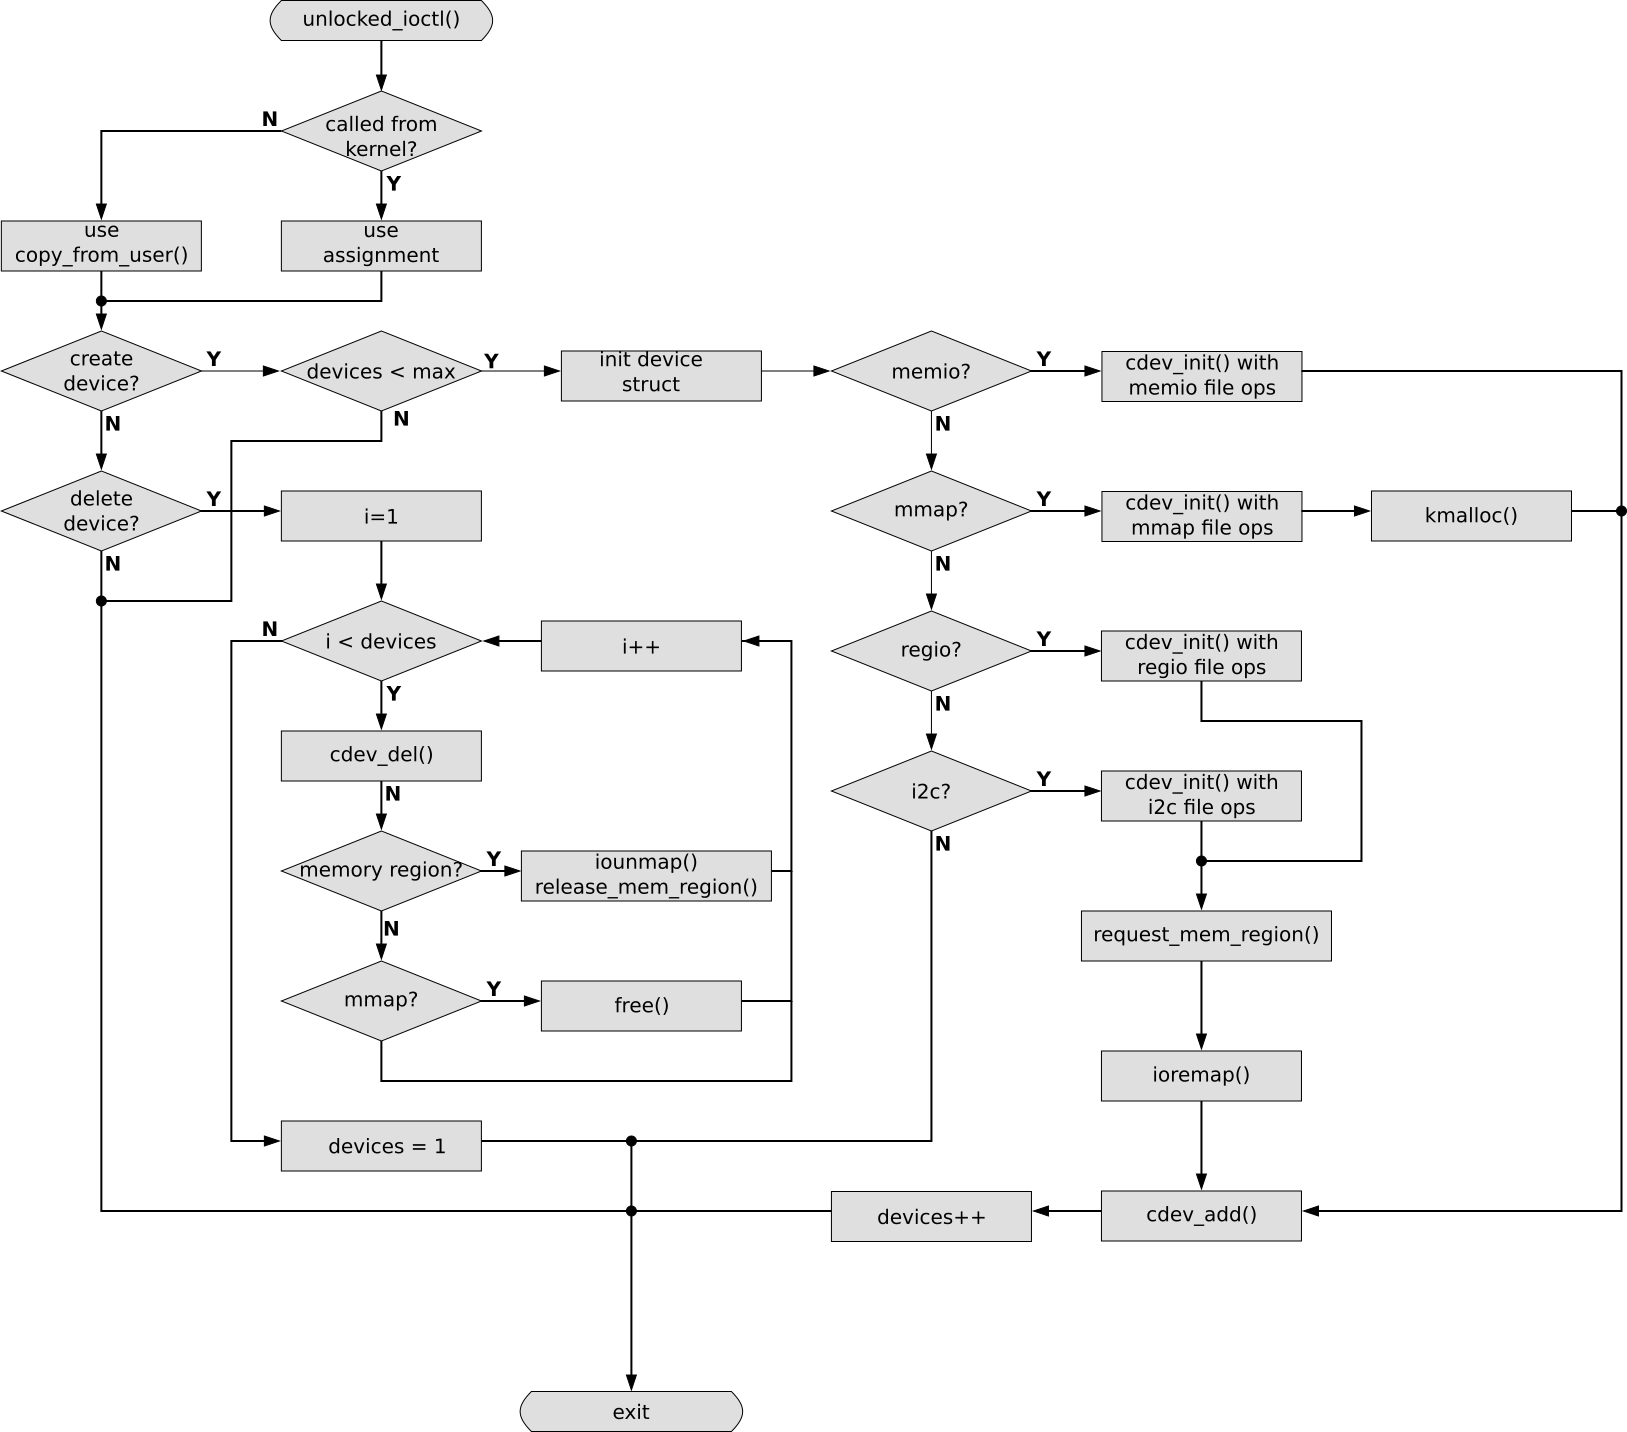
\includegraphics[width=\textwidth,height=\textheight,keepaspectratio]{figs/control_dev.png}
    \caption{Flow chart of the unlocked\_ioctl file operation for the control device}
    \label{fig:control-dev}
\end{figure}


\subsection{Interrupts}
\label{device_driver:interrupts}

\subsubsection{Kernel Timer}

For introducing interrupts to the \texttt{as\_driver}, a global timer has been added for periodically generating interrupt events. 
The timer \texttt{interrupt\_timer} is of the type \texttt{struct timer\_list}, which is part of the timer API of the kernel. 
The timer uses jiffies for determining its interval between interrupt events. 
For the Zynq platform, the default setting of the system uses the value 100 for its HZ definition (param.h which is part of the system). 
This results in a granularity for the timer interval of 10 ms. 
The timer is initialized upon loading the device driver into the kernel, where the parameter \texttt{TIMER\_INTERVAL} is used for the actual interval of the timer. 
For its interrupt handler, the timer is associated with the function \texttt{timer\_callback}, which is called when the timer expires, i.e. after the configured interval. 
The timer is triggered for the first time at the end of the initialization of the device driver and registers itself within its interrupt routine. 
In order to prevent race conditions when the device driver is unloaded, the flag \texttt{timer\_shutdown} is used. This flag is set exit method of the device driver before trying to delete the timer. 
The timer checks this flag before trying to register itself to run again. 
If this flag is set, the timer does not run again.

As aforementioned, the main purpose of the interrupt handler is to manage blocking \texttt{as\_memio} and \texttt{as\_mmap} devices. 
Since interrupt routines have to be executed in a timely manner, the amount of operations of it are rather limited. As \texttt{as\_driver} may utilize several devices, serving them can be time consuming task and is therefore not suited to be performed within the interrupt handler itself.
For this reason, the shared work queue by the kernel is used, into which the work item \texttt{timer\_wq}, is inserted. 
This work item is associated with a function, which is executed when the work item is scheduled to run by the work queue. 
The function in turn is used for carrying out the actual operations required for handling the \texttt{as\_memio} and \texttt{as\_mmap} devices. 
The work item is set up and associated with the function \texttt{data\_transfer\_update\_task} by calling the macro \texttt{INIT\_WORK}. 
The function is then scheduled by the \texttt{timer\_callback} function of the timer.
This allows the interrupt handler of the timer to return in a timely manner, since the only two operations performed by it is calling \texttt{schedule\_work} for the inserting the work item into the queue and registering itself to run again. 
The initialization of the work item is done just before configuring the timer, in order to be used.

The first part of the \texttt{data\_transfer\_update\_task} function handles any \texttt{as\_memio} devices, which are currently in use. 
In a first step, the function iterates all currently initialized devices within the \textit{device array} to find \texttt{as\_memio} devices. 
This is determined by examining the \texttt{fops} field of the device structure, whether it points to the file operation structure used for the \texttt{as\_memio} device. 
If this is the case, it checks if the \texttt{memio\_active} flag is set, which means the user has called open on the corresponding device. 
Subsequently, the \texttt{register\_intr} flag has been set, if the device is currently sleeping. 
The \texttt{data\_transfer\_update\_task} sets the condition variable \texttt{wake\_up\_cond} and calls \texttt{wake\_up\_interruptible} on the device, which causes it to wake up and check if new data has become available. 
For \texttt{as\_memio} devices which are in use but the \texttt{register\_intr} flag has not been set, the function \texttt{as\_memio\_hw\_update} of the \texttt{as\_memio} module driver is called. 
This guarantees, that data in the \textit{Ring Buffer} is not "stuck" for an extended period of time, before being transferred. 
Otherwise the user may wait indefinitely for the data to actually appear on memory or at the processing chain on the FPGA.
For the \texttt{as\_mmap} devices, the \texttt{fops} field is also checked for determining the device. 
This is performed at the same time as for the \texttt{as\_memio} devices, to prevent having to loop the devices twice. 
Similar to the \texttt{as\_memio} device, the \texttt{register\_intr} flag is examined before setting the \texttt{wake\_up\_cond} variable and calling \texttt{wake\_up\_interruptible} on the \texttt{as\_mmap} device.

\subsubsection{Hardware Module}
%TBD ?!

\construction{section}


\subsection{Driver Initialization and Deinitialization}
Once \texttt{as\_driver} has been successfully compiled, it can be loaded as a kernel module.
The device driver requests a single major number and the configured amount of minor numbers, starting with 0.
The major number is used to tell the kernel which driver is associated with a given device.
Since a device driver may be responsible for more than one device, as is the case for the \asterics device driver, the minor number is used to distinguish between the devices.
Currently, the device driver is assigned a major number dynamically by the operating system, instead of having it request a specific number itself.
This prevents potential conflicts with other drivers, if the requested major number is already in use or a different driver tries to request the same major number at a later point.
After the major number and minor numbers have been acquired, a device class is created for grouping the devices.\newline

Since the devices depend on a specific \asterics-chain, they have to be created dynamically by the \texttt{as\_control} device.
For this reason, the device driver creates the \texttt{as\_control} device upon initialization and assigns the first minor number (0) to it.
The \texttt{as\_control} device is created, by initializing the first device in the device list as the \texttt{as\_control} device.
Additionally, the number of initialized devices is incremented by one.
However, the device driver does not create a device node on the file system itself, in order for the user to choose the name and location on his own.
Rather, the user is expected to create the device node to the actual device.

Lastly, the interrupt timer is set up by mapping its service routine and configuring the time interval, at which the service routine is to be executed.
The time interval can be configured as part of the compile-time options of \texttt{as\_driver}.

As for unloading the \asterics device driver, the \texttt{timer\_shutdown} flag is set to prevent the interrupt timer to run again before deleting it using \texttt{del\_timer\_sync}.
Subsequently, all currently initialized devices, except for the \texttt{as\_control} device, are deleted by releasing all resources to the operating system and removing any memory mappings, first.
After this step, the device driver requests the kernel to delete the devices with their corresponding minor number.
Once their is no device remaining, the \texttt{control} device is deleted in the same way, before the \textit{device class} is destroyed and the driver itself is unregistered.
The major number and all minor numbers are released and may be assigned to a different driver.


\subsection{Application Notes}

\subsubsection{Building the Kernel Module}
There are two options for building the Linux kernel module, either using a cross-compiler on the host platform or the native compiler on the target platform itself.
Both require the proper \textit{kernel headers} to be installed (usually at "/lib/modules") for building Linux kernel modules for the target architecture.
A \texttt{Makefile} is provided for the \texttt{as\_driver} with options for building the Linux kernel module on either the host or the target.
Comments within the \texttt{Makefile} describe how either one can be used.
The option for compiling on the host platform, however, has only been tested for Xilinx platforms so far.
Xilinx ships ships its own libraries and tools, such as the compiler.
Additional steps may be required for other vendors but should work in the same manner, by simply referring to the path where the kernel headers have been installed.

More information for installing the kernel headers are provided at the \href{http://ti-wiki.informatik.hs-augsburg.de/doku.php?id=linux_microzed}{\textit{Technical Wiki}}.

\subsubsection{Creating Devices}
Except for \texttt{as\_control}, all devices have to be created within \texttt{as\_driver} since they depend on the actual \asterics-chain.
Devices are defined within \texttt{as\_hardware.c}, which provides interfaces for obtaining the number and list of devices.
The source file \texttt{create-devices.c} shows the required steps for creating and deleting devices using the interfaces of \texttt{as\_hardware.c(/h)}.
This file can be found at "tools/as-linux/src/kernel\_module/create-devices"
The shell script files \texttt{load\_devices.sh} and \texttt{unload\_devices.sh} use the executable of \texttt{create-devices.c}.

The whole directory ("create-devices") can be copied into the one of the system for using the system specific \texttt{as\_hardware.h/c}.

\subsubsection{Creating Device Nodes}

In order to use the devices of the \asterics driver, corresponding device nodes have to be created on the file system.
The \textit{minor} numbers are assigned in the same order as the devices are created, starting with "1" ("0" is the \texttt{as\_control} device).
However, the \textit{major} number of the kernel module has to be looked up, since it is dynamically assigned by the Linux kernel.
This can be achieved by searching for \texttt{as\_driver} in "/proc/devices".
The actual device node is then created with \textit{mknod}.

The two shell scripts \texttt{load\_devices.sh} and \texttt{unload\_devices.sh} are provided for creating and deleting device nodes.
The \textit{minor} numbers of the device nodes have to match the devices listed in \texttt{as\_hardware.c}.
 



%%%%%%%%%%%%%%%%%%%%%%%%%%%%%%%%%%%%%%%%%%%%%%%%%%%%%%%%%%%%%%%%%%%%%%%%%%%%%%
%%
%% This file is part of the ASTERICS Framework. 
%%
%% Copyright (C) Hochschule Augsburg, University of Applied Sciences
%% Efficient Embedded Systems Group
%%
%% Author(s): Gundolf Kiefer <gundolf.kiefer@hs-augsburg.de>
%%
%%%%%%%%%%%%%%%%%%%%%%%%%%%%%%%%%%%%%%%%%%%%%%%%%%%%%%%%%%%%%%%%%%%%%%%%%%%%%%



%%%%%%%%%%%%%%%%%%% 5. Interfaces %%%%%%%%%%%%%%%%%%%


\chapter{Interfaces} \label{ch:05-interfaces}

%%%%%%%%%%%%%%%%%%%%%%%%%%%%%%%%%%%%%%%%%%%%%%%%%%%%%%%%%%%%%%%%%%%%%%%%%%%%%%
%%
%% This file is part of the ASTERICS Framework. 
%%
%% Copyright (C) Hochschule Augsburg, University of Applied Sciences
%% Efficient Embedded Systems Group
%%
%% Author(s): Gundolf Kiefer <gundolf.kiefer@hs-augsburg.de>
%%            Philip Manke <philip.manke@hs-augsburg.de>
%%
%%%%%%%%%%%%%%%%%%%%%%%%%%%%%%%%%%%%%%%%%%%%%%%%%%%%%%%%%%%%%%%%%%%%%%%%%%%%%%



\section{General Interfaces} \label{ch:05-01-interfaces-general}

\secauthor{Alexander Zöllner, Gundolf Kiefer}


\subsection{Common Control and Status Registers} \label{ch:05-01-interfaces-general-common}

\infobox{Note: The following base registers are currently planned and will be integrated into the Automatics system generator in future version of \asterics.}

\begin{longtable}[ht]{|l|l|l|l|}
    \hline
    \multicolumn{1}{|c|}{\textbf{Name}} & \multicolumn{1}{c|}{\textbf{Address Off.}} & \multicolumn{1}{c|}{\textbf{Width}} & \multicolumn{1}{c|}{\textbf{Description}}\\
    \hline
    
    \texttt{asterics\_id} & 0x0 & 32 & \parbox{7cm}{\ \\
        Indicates whether the processing chain is \asterics-based.\\
    }\\
    \hline
    
    \texttt{asterics\_version} & 0x4 & 32 & \parbox{7cm}{\ \\
        Major, minor and revision of the \asterics installation this chain has been built with.\\
    }\\
    \hline
    
    \texttt{asterics\_driver\_id} & 0x8 & 32 & \parbox{7cm}{\ \\
        Compatible flavor of the software stack.\\
    }\\
    \hline
    
    \texttt{asterics\_state/control} & 0xC & 32 & \parbox{7cm}{\ \\
        Global \asterics-chain instructions and status information.\\
    }\\
    \hline
    
    \caption{Common control and status registers of an \asterics image processing chain.}
\end{longtable}

\begin{longtable}[ht]{|l|l|l|l|l|}
    \hline
    \multicolumn{1}{|c|}{\textbf{Field Name}} & \multicolumn{1}{c|}{\textbf{Bit Index}} & \multicolumn{1}{c|}{\textbf{Type}} & \multicolumn{1}{c|}{\textbf{Description}}\\
    \hline
    \texttt{asterics\_id} & 31:0 & ro & \parbox{5cm}{\ \\
        The identification field of \asterics (for example: 0x0ee500a5).\\
    }\\
    \hline
    \caption{Bit fields of the \texttt{asterics\_id} register of the \asterics-chain.}
    \label{table:common-control_asterics_id}
\end{longtable}

\begin{longtable}[ht]{|l|l|l|l|l|}
    \hline
    \multicolumn{1}{|c|}{\textbf{Field Name}} & \multicolumn{1}{c|}{\textbf{Bit Index}} & \multicolumn{1}{c|}{\textbf{Type}} & \multicolumn{1}{c|}{\textbf{Description}}\\
    \hline
    
    \texttt{major} & 31:16 & ro & \parbox{5cm}{\ \\
        Major number of the \asterics installation.\\
    }\\
    \hline
    
    \texttt{minor} & 15:8 & ro & \parbox{5cm}{\ \\
        Minor number of the \asterics installation.\\
    }\\
    \hline
    
    \texttt{revision} & 7:0 & ro & \parbox{5cm}{\ \\
        Revision of the \asterics installation.\\
    }\\
    \hline

    \caption{Bit fields of the \texttt{asterics\_version} register of the \asterics installation.}
    \label{table:common-control_asterics_version}
\end{longtable}

\begin{longtable}[ht]{|l|l|l|l|l|}
    \hline
    \multicolumn{1}{|c|}{\textbf{Field Name}} & \multicolumn{1}{c|}{\textbf{Bit Index}} & \multicolumn{1}{c|}{\textbf{Type}} & \multicolumn{1}{c|}{\textbf{Description}}\\
    \hline
    
    \texttt{driver\_id} & 31:0 & ro & \parbox{5cm}{\ \\
        Identification number of compatible software stack flavor.\\
        First 8 characters of the SHA1 hash of \texttt{as\_hardware.c}.\\
    }\\
    \hline
    
    \caption{Bit fields of the combined \texttt{asterics\_driver\_id} register of the \asterics-chain.}
    \label{table:common-control_asterics_driver_id}
\end{longtable}

\begin{longtable}[ht]{|l|l|l|l|l|}
    \hline
    \multicolumn{1}{|c|}{\textbf{Field Name}} & \multicolumn{1}{c|}{\textbf{Bit Index}} & \multicolumn{1}{c|}{\textbf{Type}} & \multicolumn{1}{c|}{\textbf{Reset Value}} & \multicolumn{1}{c|}{\textbf{Description}}\\
    \hline
    
    \texttt{reset} & 16 & wo & 0x0 & \parbox{5cm}{\ \\
        Reset the entire \asterics-chain at once.\\
    }\\
    \hline
    
    \texttt{sync\_error} & 3 & ro & 0x0 & \parbox{5cm}{\ \\
        Data synchronization error occurred anywhere within the \asterics-chain which led to data loss.\\
    }\\
    \hline
    
    \texttt{data\_error} & 2 & ro & 0x0 & \parbox{5cm}{\ \\
        A data error occurred anywhere within the \asterics-chain.\\
    }\\
    \hline
    
    \texttt{ready} & 0 & ro & n/a & \parbox{5cm}{\ \\
        \asterics-chain is ready for operation.\\
    }\\
    \hline
    
    \caption{Bit field overview of the combined \texttt{asterics\_state/control} register of the \asterics-chain.}
    \label{table:common-control_asterics_state_control}
\end{longtable}

The \texttt{READY} signal described in Table~\ref{table:common-control_asterics_state_control} is a "AND" combination of the \texttt{READY} signals of all hardware modules.
Similarly, the \texttt{DATA\_ERROR} and \texttt{SYNC\_ERROR} signal are "OR" combinations of their respective signals of all hardware modules.

Usually, the hardware modules also poses a \texttt{state/control} register with the same bit fields as the \texttt{asterics\_state/control} register.

\subsection{Error Handling}

There are two distinct error types available to \asterics, namely \texttt{SYNC\_ERROR} and \texttt{DATA\_ERROR}, which are handled separately.
The former is a per-module signal, as described in Table~\ref{05-02-module_signals} of Chapter~\ref{ch:05-02-interfaces-module_signals}, which may be forwarded to the \texttt{asterics\_state/control} register of the \asterics-chain.
The \texttt{SYNC\_ERROR} cannot be cleared by software directly. Rather, a reset has to be performed on the \asterics-chain (see Chapter~\ref{ch:05-02-interfaces-module_signals-error_handling}).
 
The \texttt{DATA\_ERROR} is part of the \texttt{as\_stream} interface (see Chapter~\ref{ch:05-03-interfaces-as_stream}).
As opposed to the \texttt{SYNC\_ERROR}, the software is responsible for clearing the \texttt{DATA\_ERROR}, as described in Chapter~\ref{ch:05-03-interfaces-as_stream-error_handling}.


\subsection{Module and Chain Reset Behavior}

Under certain circumstances, the need for reseting the \asterics image processing chain may arise, for example for having a defined state of the processing chain before using it for the first time or if an error occurred.

An \asterics-chain can either be reset at once using the \texttt{RESET} signal of the \texttt{asterics\_control} register or per-module.
The latter requires to perform the reset in the correct order, starting from the data source to sink.

If a module receives a \texttt{RESET} signal, the corresponding \texttt{READY} and \texttt{STROBE} signals have to be unset (0) after the following clock cycle.
\texttt{READY} and \texttt{STROBE} must not be set (1) as long as \texttt{RESET} is set (1).
The \texttt{RESET} signal has to persist for at least one clock cycle.
Once the \texttt{RESET} is unset (0), the module sets its \texttt{READY} signal as soon as data can be accepted or the \texttt{STALL} signal can be set correctly.

The software is expected to read the \texttt{READY} signal of all modules or the one of the \texttt{asterics\_state} register before starting any module.

\subsection{Version Management}

\asterics allows to build a wide variety of image processing chains, each being accompanied with their own \textit{\asterics Support Package}.
Thus, the \textit{\asterics Support Package} has to match the configuration of the \asterics-chain, which includes address offsets or the type of modules which have been used.
If the software does not match the hardware, unexpected behavior or the \asterics-chain not working at all is to be expected.
The most common error is software drivers trying to access the module's corresponding hardware registers at a certain address but inadvertently configure registers of a different type due to mismatch of addresses.

For this reason, the \asterics-chain poses version registers as described in Chapter~\ref{ch:05-01-interfaces-general-common}.
The software can read these registers to check whether the current version of the software stack is compatible with the \asterics-chain it is trying to operate.

The \textit{\asterics Support Package} also poses a version, which is a SHA1 hash of the source file \texttt{as\_hardware.c}.
This file describes the configuration of the \asterics-chain, along with pre-synthesis parameters of the used modules.



\subsection{\textit{i2c} Bus Master for Module Configuration}

\secauthor{Philip Manke}

%[[ TBD (PM): Prinzipielle Einführung, wie Module mit i2c-Slave-Schnittstelle %angebunden werden (Schnittstellen-Sicht); Details im Kapitel "Modules" (s.u.) ]]


External modules used with the \asterics framework (particularly cameras) often require to be configured using the \textit{i2c} bus. To provide a universal solution across platforms for this problem, \asterics implements its own \textit{i2c} hardware module.

This section will give a brief overview on what \textit{i2c} is and how to get started using the \texttt{as\_iic} module. 

\subsubsection{What is \textit{i2c}?}

\textit{i2c} is a bus system which allows for multiple devices to be connected using just two signals/wires in total. There are two types of devices which connect to the bus: masters and slaves.
Only masters are allowed to start a transaction on the bus. Having multiple masters on a single bus is not supported by the \texttt{as\_iic} module, though generally possible.

The two wires of the \textit{i2c} bus carry a clock signal (SCL \^= Serial CLock) and a data signal (SDA \^= Serial DAta).

The \textit{i2c} protocol uses device addresses to talk to the different devices on the bus. This address is 8 bits in length, with the last bit differentiating between read and write transactions.

\subsubsection{How to Configure \texttt{as\_iic} for Operation}

The \texttt{as\_iic} module only requires one function to be run before it is fully operational: \texttt{as\_iic\_init()}.
This configures the SCL frequency of the \textit{i2c} bus and is effective immediately.
The supported standard \textit{i2c} bus frequencies are 100 kHz and 400 kHz for \textit{standard mode} and \textit{fast mode i2c} respectively. With the \texttt{as\_iic} module it is possible to configure the frequency freely in a range from 10 kHz to 1 MHz.
This allows for faster transactions, provided the slave devices support the faster bus frequency. 
The function \texttt{as\_iic\_reset()} resets the module to the uninitialized state.

\subsubsection{Using \texttt{as\_iic}}

The software driver for \texttt{as\_iic} provides easy-to-use high level functions for executing transactions on the \textit{i2c} bus.
After connecting the hardware and initializing the \texttt{as\_iic} module correctly, the high level driver functions can be used immediately.

The two most useful functions are:

\begin{itemize}
    \item \texttt{as\_iic\_read\_reg()}
    \item \texttt{as\_iic\_write\_reg()}
\end{itemize}

These two functions will read and write the registers of \textit{i2c} slaves connected to the bus.
They both need the \textit{i2c} modules' base-address, the \textit{i2c} address of the slave and a pointer to the address of the register to read or write.
The forth pointer required by the functions points to the byte to send to the \textit{i2c} slave (\texttt{as\_iic\_write\_reg()}) or to the variable to store the content of the \textit{i2c} slave register in (\texttt{as\_iic\_read\_reg()}).

Section \ref{07-05-as-iic-connect-devices} briefly describes how to connect hardware devices to the \textit{i2c} bus. 

Details on the software driver for \texttt{as\_iic} and other modules, can be found in the \asterics Doxygen documentation.
The implementation of \texttt{as\_iic} is explained in detail in \ref{ch:07-05-modules-i2c}.

It is recommended to check out \ref{07-05-04-as-iic-quirks} before using \texttt{as\_iic}, to avoid common pitfalls.


\subsection{Generic Register Interface for \asterics Modules}
\label{sec:05-01-05-register_interface}
\secauthor{Philip Manke}

\asterics provides a generic and configurable register interface that all modules can use.
Configuring it becomes very easy when used in conjunction with Automatics, the \asterics chain generator.
Table \ref{table:05-01-slave_register_interface_signals} lists the ports comprising the slave register interface from the viewpoint of an ASTERICS module.

\begin{longtable}[ht]{|l|l|l|l|}
    \hline
    \multicolumn{1}{|c|}{\textbf{Name}} & \multicolumn{1}{c|}{\textbf{Data Type}} & \multicolumn{1}{c|}{\textbf{Direction}} & \multicolumn{1}{c|}{\textbf{Description}}\\
    \hline
    
    \texttt{slv\_status\_reg} & \texttt{slv\_reg\_data} & out & \parbox{6cm}{\ \\
        Data transport to software. An array of 32 bit registers.\\
    }\\
    \hline
    
    \texttt{slv\_ctrl\_reg} & \texttt{slv\_reg\_data} & in & \parbox{6cm}{\ \\
        Data transport to hardware. An array of 32 bit registers.\\
    }\\
    \hline
    
    \texttt{slv\_reg\_modify} & \texttt{std\_logic\_vector} & out & \parbox{6cm}{\ \\
        Data modify enable signals for the status registers. A vector as wide as the number of registers. Every clock cycle that a bit is set to \texttt{'1'} in this vector, the register will update it's value as set from the hardware.\\
    }\\
    \hline
    
    \texttt{slv\_reg\_config} & \texttt{slv\_reg\_config\_table} & out & \parbox{6cm}{\ \\
        A port to export the register configuration. An array of two bit \texttt{std\_logic\_vectors}, designating how the registers are configured.\\
    }\\
    \hline
    
    \caption{Overview of the signals comprising the slave register interface of \asterics modules.}
    \label{table:05-01-slave_register_interface_signals}
\end{longtable}

Each module using the interface must implement all four ports.
The \texttt{helpers} package from the \texttt{asterics} library must also be used in the VHDL file.
This makes the custom data types used to bundle the register signals available within the module.

Additionally, the module must contain a constant named \texttt{slave\_register\_configuration} towards the top of the architecture defintion:\\
\texttt{constant slave\_register\_configuration : slv\_reg\_config\_table(0 to <reg\_count>) := (<config>)}

The width of the constant and all ports must manually be set to the number of the desired register count.
Then the constant can be configured:
For each register a two bit wide \texttt{std\_logic\_vector} is required, table \ref{table:05-01-slave_register_config_values} lists all possible values.

\begin{longtable}[ht]{|c|c|}
    \hline
    \textbf{Value} & \textbf{Description}\\
    \hline
    
    \texttt{AS\_REG\_NONE} or \texttt{"00"} & \parbox{11cm}{\ \\
        No register generated.\\
    }\\
    \hline
    
    \texttt{AS\_REG\_STATUS} or \texttt{"01"} & \parbox{11cm}{\ \\
        Only generate a status register: Data transport only from the hardware module to the software. This saves some hardware resources and increases data security, as the software won't be able to overwrite the register contents.\\
    }\\
    \hline
    
    \texttt{AS\_REG\_CONTROL} or \texttt{"10"} & \parbox{11cm}{\ \\
        Only generate a control register: Data transport only from software towards the hardware module. This mainly just saves some hardware resources.\\
    }\\
    \hline
    
    \texttt{AS\_REG\_BOTH} or \texttt{"11"} & \parbox{11cm}{\ \\
        Generate a full slave register with data transport enabled in both directions.\\
    }\\
    \hline
    
    \caption{Possible values in the slave register configuration constant.}
    \label{table:05-01-slave_register_config_values}
\end{longtable}


\textbf{Example configuration:}\\
\texttt{constant slave\_register\_configuration : slv\_reg\_config\_table(0 to 3) := ("11", "11", "10", "01");}\\
For this configuration, all ports also need to have a data width of \texttt{(0 to 3)}. Also note that all register ports and the constant have data widths in an ascending direction (using \texttt{to} instead of \texttt{downto})!

\textbf{Note:} You may use an "others" construct to assign the register configuration (\texttt{:= ("11", (others => "01"))}. This is supported by Automatics for automatic IP-Core generation. \textit{Important:} This causes an error when using the constant definitions \texttt{AS\_REG\_XX} and may thus only be used with string literals (eg. \texttt{"01"})!

\textbf{Note:} If the module only has a single register, the "normal" assignment of the configuration constant using \texttt{:= ("10")} will usually fail. Either use an \texttt{others} construct or a direct assignment using \texttt{:= (0 => "10")} to assign the register configuration. Both ways are supported by Automatics.

\bigskip

\textbf{Using Automatics:}

Automatics can automatically instantiate the required register manager for the register interface.
This requires the following:
\begin{itemize}
\item The ports of the register interface must contain the names as mentioned above. They may have a \textit{common suffix}, which is required if a module contains multiple interfaces. The suffix must be separated by an underscore from the specified signal names and the configuration constant must have the same suffix. Note: The suffix is only required if the module has multiple register interfaces.
\item The configuration constant must be defined in the architecture definition, before any \texttt{begin} keyword, as Automatics stops parsing the architecture at the first \texttt{begin} keyword.
\end{itemize} 

\textbf{Manual configuration:}

The register interface ports must be connected to the register manager component \texttt{as\_regmgr}.
The register manager has an interface consisting of the same ports with identical names as the register interface of the hardware modules:
\begin{itemize}
\item \texttt{slv\_status\_reg => slv\_status\_reg}
\item \texttt{slv\_ctrl\_reg => slv\_ctrl\_reg}
\item \texttt{slv\_reg\_modify => slv\_reg\_modify}
\item \texttt{slv\_reg\_config => slv\_reg\_config}
\end{itemize}
\bigskip

And an interface roughly matching an AXI interface, ommiting unnecessary signals.
Table \ref{table:05-01-slave_register_axi_signals} lists these ports.
\begin{longtable}[ht]{|l|l|l|l|}
    \hline
    \multicolumn{1}{|c|}{\textbf{Name}} & \multicolumn{1}{c|}{\textbf{Data Type}} & \multicolumn{1}{c|}{\textbf{Direction}} & \multicolumn{1}{c|}{\textbf{Description}}\\
    \hline
    
    \texttt{sw\_address} & \texttt{std\_logic\_vector} & in & \parbox{6cm}{\ \\
        The read and write address. \texttt{as\_regmgr} does NOT support simultanious read and write accesses.\\
    }\\
    \hline
    
    \texttt{sw\_data\_out} & \texttt{std\_logic\_vector} & out & \parbox{6cm}{\ \\
        Data transport towards software.\\
    }\\
    \hline
    
    \texttt{sw\_data\_in} & \texttt{std\_logic\_vector} & in & \parbox{6cm}{\ \\
        Data transport towards hardware modules.\\
    }\\
    \hline
    
    \texttt{sw\_data\_out\_en} & \texttt{std\_logic} & in & \parbox{6cm}{\ \\
        Enable signal for read accesses from software.\\
    }\\
    \hline
    
    \texttt{sw\_data\_in\_en} & \texttt{std\_logic} & in & \parbox{6cm}{\ \\
        Enable signal for write accesses from software.\\
    }\\
    \hline
    
    \texttt{sw\_byte\_mask} & \texttt{std\_logic\_vector} & in & \parbox{6cm}{\ \\
        Byte-wise mask for partial write operations. Fully supported by \texttt{as\_regmgr}.\\
    }\\
    \hline
    
    \caption{Overview of the signals comprising the ports connected to the AXI Slave manager of the \asterics slave register manager.}
    \label{table:05-01-slave_register_axi_signals}
\end{longtable}


\textbf{Integration details:}

The software address is only as wide as the addressing of the hardware modules requires.
Therefore the required bits have to be extracted from the address provided by the AXI Slave manager.
The address will also have to be multiplexed from the read and write addresses.

The \texttt{sw\_data\_out} signal will also have to be multiplexed towards software (the AXI Slave manager).

Static HDL code has been developed and is used by Automatics to accomplish these tasks, shown in listing \ref{Code:05-01-06-regmgr_static}.
Note that the constants have to be assigned values chosen for the system that the code is used in.

\begin{lstlisting}[style=hdl, label=Code:05-01-06-regmgr_static, caption=Static code used to manage multiple \texttt{as\_regmgr} modules]
  -- Register interface constants and signals:
  -- Register address width in as_regmgr
  constant c_slave_reg_addr_width : integer := 6;
  -- Module addressing width: ceil(log2(module count))
  constant c_module_addr_width: integer := 2;
  -- Register addressing width: ceil(log2(register count per module))
  constant c_reg_addr_width : integer := 4;
  -- Number of as_regmgrs
  constant c_reg_if_count : integer := 4;
  -- Which module / as_regmgr is addressed?  
  signal read_module_addr : integer;
  -- Current address for as_regmgrs
  signal sw_address : std_logic_vector
                        (c_slave_reg_addr_width - 1 downto 0);
  -- Collect the sw_data_out signals of all as_regmgrs
  signal mod_read_data_arr : slv_reg_data(0 to c_reg_if_count - 1);

begin

  -- Extract the module address from the AXI read address
  read_module_addr <= to_integer(unsigned(
    axi_slv_reg_read_address(c_slave_reg_addr_width + 1 
                               downto c_reg_addr_width + 2)));

  -- Connect the read data out port
  --    of the register manager of the addressed module
  read_data_mux : process(mod_read_data_arr, read_module_addr, reset_n)
  begin
      if reset_n = '0' then
          axi_slv_reg_read_data <= (others => '0');
      else
          if read_module_addr < c_reg_if_count 
                and read_module_addr >= 0 then
              axi_slv_reg_read_data <= 
                  mod_read_data_arr(read_module_addr);
          else
              axi_slv_reg_read_data <= (others => '0');
          end if;
      end if;
  end process;

  -- Select between read and write address of the AXI interface
  --   depending on the read/write enable bits
  -- The register managers can only handle a single
  --   read/write per clock cycle
  -- Write requests have priority
  sw_addr_mux:
  process(axi_slv_reg_write_address, axi_slv_reg_read_address, 
            axi_slv_reg_write_enable, axi_slv_reg_read_enable)
  begin
    sw_address <= (others => '0');
    -- Disregarding lowest two bits
    --   to account for byte addressing on 32 bit registers
    if axi_slv_reg_write_enable = '1' then
        sw_address <= axi_slv_reg_write_address
                        (c_slave_reg_addr_width + 1 downto 2);
    elsif axi_slv_reg_read_enable = '1' then
        sw_address <= axi_slv_reg_read_address
                        (c_slave_reg_addr_width + 1 downto 2);
    else
        sw_address <= (others => '0');
    end if;
  end process;
\end{lstlisting}

\bigskip

The register managers have five Generics, configuring data widths and which address they should listen for, listed in table \ref{table:05-01-slave_register_manager_generics}.

\begin{longtable}[ht]{|l|l|l|l|}
    \hline
    \multicolumn{1}{|c|}{\textbf{Name}} & \multicolumn{1}{c|}{\textbf{Data Type}} & \multicolumn{1}{c|}{\textbf{Default Value}} & \multicolumn{1}{c|}{\textbf{Description}}\\
    \hline
    
    \texttt{REG\_ADDR\_WIDTH} & \texttt{integer} & 12 & \parbox{6cm}{\ \\
        The register address width: ceil(log2(number of register managers)) + ceil(log2(number of registers per module)).\\
    }\\
    \hline
    \texttt{REG\_DATA\_WIDTH} & \texttt{integer} & 32 & \parbox{6cm}{\ \\
        The register data width. Usually 32 bit.\\
    }\\
    \hline
    \texttt{MODULE\_ADDR\_WIDTH} & \texttt{integer} & 6 & \parbox{6cm}{\ \\
        Number of bits used to address \texttt{as\_regmgr} in this system.\\
    }\\
    \hline
    \texttt{REG\_COUNT} & \texttt{integer} & 32 & \parbox{6cm}{\ \\
        The number of registers for this \texttt{as\_regmgr}.\\
    }\\
    \hline
    \texttt{MODULE\_BASEADDR} & \texttt{integer} & None & \parbox{6cm}{\ \\
        The address for this \texttt{as\_regmgr}.\\
    }\\
    \hline
    
    \caption{Overview of Generics of the \asterics slave register manager.}
    \label{table:05-01-slave_register_manager_generics}
\end{longtable}

%%%%%%%%%%%%%%%%%%%%%%%%%%%%%%%%%%%%%%%%%%%%%%%%%%%%%%%%%%%%%%%%%%%%%%%%%%%%%%
%%
%% This file is part of the ASTERICS Framework. 
%%
%% Copyright (C) Hochschule Augsburg, University of Applied Sciences
%% Efficient Embedded Systems Group
%%
%% Author(s): Gundolf Kiefer <gundolf.kiefer@hs-augsburg.de>
%%
%%%%%%%%%%%%%%%%%%%%%%%%%%%%%%%%%%%%%%%%%%%%%%%%%%%%%%%%%%%%%%%%%%%%%%%%%%%%%%



\section{Common Per-Module Signals} \label{ch:05-02-interfaces-module_signals}

\secauthor{Gundolf Kiefer}

\subsection{Signal Overview}

Table~\ref{05-02-module_signals} shows the common signals that should be present in every\asterics module. Optional signals are marked with an asterisk (*). The column "Default" denotes the value that should be assumed for outer modules if the respective signal is absent.

All \asterics chains are synchronous designs the one common clock signal \texttt{CLK} with all flipflops being triggered with the raising edge of \texttt{CLK}. Unless noted otherwise, all other signals are active-high.

\begin{longtable}[ht]{|c|c|c|c|}
\hline 
\textbf{Signal} & \textbf{Direction} & \textbf{Default} & \textbf{Description} \\
% (* = optional) & (in / out) & (if optional) & \\
\hline
\hline
\endhead

\texttt{RESET} (*) & in & 0 &
\parbox{7cm}{ ~ \\ Reset the module. \\ ~ \\ \small
This signal may only be omitted if the module is purely combinational.
If set for 1 clock cycle, the module must reset itself.
\\ ~ } \\

\hline 

\texttt{READY} (*) & out & 1 &
\parbox{7cm}{ ~ \\ Module is ready to operate. \\ ~ \\ \small
This is the response signal to RESET. If the reset process requires more than 1 clock cycle, the module may keep the READY signal low until the module is ready for normal operation. Once set (1), the module is not allowed to unset the signal unless a reset request was received.
The READY signal may be omitted if the module is purely combinational or if the reset process is guaranteed to complete within one clock cycle.
\\ ~ } \\

\hline 

\texttt{SYNC\_ERROR} (*) & out & 0 &
\parbox{7cm}{~ \\ A Synchronization error occured. \\ ~ \\ \small
If the module encounters an error related to a potential loss of data or synchronization information, the module must raise this signal. At the same time, the module must go into a fail-safe state in which it does not generate any out potentially unexpected for subsequent modules. The SYNC\_ERROR output set to 1 and the fail-safe behaviour must persist until the
RESET input is set.
\\ ~ } \\

\hline 

\texttt{FLUSH} (*) & in & 1 &
\parbox{7cm}{~ \\ Write out all internal buffers. \\ ~ \\ \small
All modules with internal buffers that do not flush automatically must implement this signal.
If set, the module processes all internally buffered data, regardless whether new input data is arriving. If the signal is unset again while there is still data buffered, the module should, but is not required to stop processing.
\\ ~ } \\

\hline 

\caption{Per-Module Signals ( (*) = optional)} \label{05-02-module_signals}\\
\end{longtable}



\subsection{Module Reset and Error Handling} \label{ch:05-02-interfaces-module_signals-error_handling}

The signals \texttt{RESET}, \texttt{READY}, and \texttt{SYNC\_ERROR} should all be made accessible to software (i.~e. as I/O register bits and as part of the module driver).

On chain level, it is recommended to introduce global signals with the same names and make them accessible via I/O register bits. The global \texttt{READY} bit should be a logical "and" of all module-level \texttt{READY} signals. The global \texttt{SYNC\_ERROR} bit should be a logical "or" of all module-level \texttt{SYNC\_ERROR} signals.

The provision of a global \texttt{RESET} signal is particularly helpful to avoid potential errors due to an incorrect reset order if the modules are reset individually by software. If a global reset mechanism is missing, the software must reset the modules in a correct topological (half-)order, starting at the input modules and proceeding towards the output modules. Otherwise, a module that has just been reset may receive input data from a not-yet reset module and get into an unwanted state or produce undesired output.



\subsection{Module Flushing}

Modules may contain internal data buffers. For example, memory writer modules collect a number of data words in order to write them out efficiently using burst transfers. 2D Window Pipelines must buffer multiple lines of image data for their operation. If a frame-oriented processing chain is operated in a single-shot mode with potentially long periods of time without new incoming frame data, it can thus happen that data of a previous frame resides inside such buffers without being processed further. In consequence, follow-up (software) modules waiting for the completion of a frame cannot proceed. In the worst case, this results in a deadlock: The application software is waiting for the \asterics chain to deliver the last results of the current frame and would trigger a new frame afterwards. The \asterics chain, on the other hand, is inactive since now new data is coming in. This, however, does not happen, because the software is waiting.

The main purpose of the \texttt{FLUSH} signal is to circumvent such deadlock conditions. If set, the module is requested to completely process all of its internal data. In particular, if a unit of data (e.g. a frame) has been received completely at the input side, all output data of that frame must be emitted at its output side.

The \texttt{FLUSH} signal should be made available both to hardware (i.~e. as an input signal) and to software (i.~e. as a bit inside a slave register). In a typical use case, it is controlled by software.

%%%%%%%%%%%%%%%%%%%%%%%%%%%%%%%%%%%%%%%%%%%%%%%%%%%%%%%%%%%%%%%%%%%%%%%%%%%%%%
%%
%% This file is part of the ASTERICS Framework. 
%%
%% Copyright (C) Hochschule Augsburg, University of Applied Sciences
%% Efficient Embedded Systems Group
%%
%% Author(s): Gundolf Kiefer <gundolf.kiefer@hs-augsburg.de>
%%
%%%%%%%%%%%%%%%%%%%%%%%%%%%%%%%%%%%%%%%%%%%%%%%%%%%%%%%%%%%%%%%%%%%%%%%%%%%%%%



\section{The \asterics Streaming Interface (\texttt{as\_stream}) } \label{ch:05-03-interfaces-as_stream}

\secauthor{Gundolf Kiefer}

\subsection{Signal Overview}

An \texttt{as\_stream} bus is used to transport mostly image, but also other types of data from one \textit{source} module to one or multiple \textit{sink} modules. The bus consists of an arbitrary number of data bits and a set of control signals.

The \texttt{as\_stream} bus signals are listed in Table~\ref{05-03-as_stream_signals}. Signals denoted with a right arrow ($\rightarrow$) in column "Direction" are outputs for the source module and inputs for the sink module(s). Accordingly, signals denoted with a left arrow ($\leftarrow$) are directed from the sink module to the source module. Presently, only the \texttt{STALL} signal is directed backwards (from sink to source). If an \texttt{as\_stream} bus connects to multiple sinks, an OR gate must be inserted to combine all their \texttt{STALL} outputs to feed the \texttt{STALL} input of the source module.

Optional signals are marked with an asterisk (*). The column "Default" denotes the value that should be connected to the input signal of a module if the respective output is missing on the peer side.

\begin{longtable}[ht]{|c|c|c|c|}
\hline 
\textbf{Signal} & \textbf{Direction} & \textbf{Default} & \textbf{Description} \\
%% \small (* = optional) & \small (source <dir> sink) & \small (if optional) & \\%%
\hline 
\hline 
\endhead

\texttt{DATA<$n$>} & $\rightarrow$ &  &
\parbox{7cm}{ ~ \\ User data. \\ ~ \\ \small
The width $n$ and the data type are application-dependent, can be chosen arbitrarily with $n \geq 1$ and are not defined by the \texttt{as\_stream} specification.
\\ ~ } \\

\hline 

\texttt{STROBE} & $\rightarrow$ & &
\parbox{7cm}{ ~ \\ A new valid data item is present at the \texttt{DATA} bus.
\\ ~ } \\

\hline 

\texttt{DATA\_ERROR} (*) & $\rightarrow$ & &
\parbox{7cm}{~ \\ The present data item is invalid/unknown.
\\ ~ } \\

\hline 

\texttt{STALL} (*) & $\leftarrow$ & 0 &
\parbox{7cm}{~ \\ Request to pause sending data. \\ ~ \\ \small
This signal allows the sink module to put back pressure on its predecessor module if it is not able to process its incoming data in time. See Section \ref{05-03-stall} for detailed explanations on the mechanism.
\\ ~ } \\

\hline 

\texttt{VSYNC} (*) & $\rightarrow$ & -- &
\parbox{7cm}{~ \\ Vertical (image) synchronization. \\ ~ \\ \small
This signal is optional. However, if it is present on the sink side, it must also be provided by the source. A clock cycle during which this signal is set marks the beginning (first pixel) of a new 2D image. \\ ~ \\
Note: Some modules may operate incorrectly if this signal is set while \texttt{STROBE=0}.
%[[ TBD: Im Wiki steht, dass STROBE auch für HSYNC/VSYNC gilt. Wäre das nicht so, könnte diese Notiz entfallen. ]]
\\ ~ } \\

\hline 

\texttt{VCOMPLETE} (*) & $\rightarrow$ & \texttt{=VSYNC} &
\parbox{7cm}{~ \\ Image transfer completed. \\ ~ \\ \small
The signal indicates that an image has just been transferred completely and serves as a hint for subsequent modules. It should ideally be set during the clock cycle immediately following the cycle during which the last data item has been transferred. \\ ~ \\
\\ ~ } \\

\hline 

\texttt{HSYNC} (*) & $\rightarrow$ & -- &
\parbox{7cm}{~ \\ Horizontal (line) synchronization. \\ ~ \\ \small
This signal is optional. However, if it is present on the sink side, it must also be provided by the source. A clock cycle during which this signal is set marks the beginning (first pixel) of a new line. \\ ~ \\
Note: Some modules may operate incorrectly if this signal is set while \texttt{STROBE=0}. 
%[[ TBD: Im Wiki steht, dass STROBE auch für HSYNC/VSYNC gilt. Wäre das nicht so, könnte diese Notiz entfallen. ]]
\\ ~ } \\

\hline 

\texttt{HCOMPLETE} (*) & $\rightarrow$ & \texttt{=HSYNC} &
\parbox{7cm}{~ \\ Line transfer completed. \\ ~ \\ \small
The signal indicates that an image has just been transferred completely and serves as a hint for subsequent modules. It should ideally be set during the clock cycle immediately following the cycle during which the last data item has been transferred.
\\ ~ } \\

\hline 

\caption{Signals of an \texttt{as\_stream} bus ( (*) = optional)} \label{05-03-as_stream_signals}\\
\end{longtable}




\subsection{General Design Rules}

\subsubsection{Registered outputs}

All output signals of an \texttt{as\_stream} port have to be driven immediately by (a) a flipflop, or (b) an input signal, if there is absolutely no logic between this input and the output (not even a single gate!). Case (b) is particularly useful for the \texttt{STALL} signal to avoid long stall latencies requiring in potentially area-consuming buffers. In all other cases, it is safe and good to just always insert flipflops at the outputs.

%\subsubsection{[[ TBD: weitere ]]}



\subsection{Error handling} \label{ch:05-03-interfaces-as_stream-error_handling}

The \texttt{DATA\_ERROR} signal indicates whether the value of a dedicated data item is incorrect or unreliable. Ideally, this information should be propagated through the whole chain up to the output, so that the application can read which parts of the data are correct and which are not.

In some cases, the \texttt{DATA\_ERROR} information cannot be propagated up to the end. Examples are: 
\begin{itemize}
\item The chain may end with an \texttt{as\_memwriter} module, and the output data format has no fields to indicate the validity of individual pixels / data units.
\item There are modules in the chain that do not support the \texttt{DATA\_ERROR} signal.
\end{itemize}
In such cases, it is recommended to add a global status register bit \texttt{GLOB\_DATA\_ERROR}, which is set to one if the last element of a chain propagating the data error information raises its \texttt{DATA\_ERROR} output and must be reset by software. This way, the application software can at least determine if some data units may be reliable between two polls of this status bit.



\subsection{Stall Mechanism} \label{05-03-stall}

The \texttt{STALL} signal enables modules which cannot guarantee to process a new input data word in each clock cycle to send a break signal towards their predecessor modules and slow them down just enough to let the whole chain operate correctly and at optimum speed.

Unlike all other signals, which are all directed forward and together allow build well-formed, very long pipelines without encountering serious physical problems, the \texttt{STALL} signal is directed backwards. To avoid over-long signal paths, it may need to be buffered and may thus require a certain (system- or chain-dependent) number of clock cycles until it is handed over from the overloaded module to the first, data-generating module of a complex chain. This must be taken into account by the chain designer, and buffer registers or FIFOs must be inserted into the chain to avoid data loss due to data latencies.

To help the chain designer in this task and to allow an automatic insertion of such buffers in the future, the following rules apply:

\begin{enumerate}

\item \texttt{STROBE} has precedence over \texttt{STALL}. A \texttt{STROBE} signal set to 1 strictly and unequivocally defines that there the \texttt{DATA} signal carries a new data item \textit{now}, which will never be repeated. The sink module must take the data or raise a \texttt{SYNC\_ERROR} condition, even if it has already set its \texttt{STALL} signal. In other words, \texttt{STALL} can be seen as a request or a hint, which may or may not be followed. Any module that cannot take over a new data item each clock cycle must be designed to deal with such a situation and do a correct \texttt{SYNC\_ERROR} error handling.

\item An \texttt{as\_stream} \textit{source} port can be \textit{stall-absorbing} or not. Whether or not a port is \textit{stall-absorbing} should be indicated by the presence of the optional \texttt{STALL} signal, which should only be present for \textit{stall-absorbing} modules. Exceptions must clearly be identified in the module documentation.

\item An \texttt{as\_stream} \textit{sink} port can be \textit{stall-generating} or not. Whether or not a port is \textit{stall-generating} should be indicated by the presence of the optional \texttt{STALL} signal, which should only be present for \textit{stall-generating} modules. Exceptions must clearly be identified in the module documentation.

\item Certain filter modules which do not need to generate stalls themselves and cannot buffer much data internally may still implement the \texttt{STALL} port signals and simply propagate the \texttt{STALL} signal from their outgoing to their incoming \texttt{as\_stream} port. Such modules are referred to as \textit{stall-propagating} modules. Towards their successor, they act as a \textit{stall-absorber}. Towards their predecessor, they act as a \textit{stall-generator}.

\item Any sink port must accept the last data unit during the clock cycle in which the \texttt{STALL} signal is raised without errors. \label{05-03-cond_stall_sink}

\item A source port which is declared to be \textit{stall absorbing} must not set its \texttt{STROBE} signal one clock cycle after which \texttt{STALL} has been raised.

\end{enumerate}

In order to fullfil the condition \ref{05-03-cond_stall_sink}, modules which forward their \texttt{STALL} signal from an output to an input must do this within the same clock cycle, i.~e. by pure combinational logic without and flipflops. This may lead to overlong combinational paths during synthesis. Timing issues can be overcome by inserting dedicated \texttt{as\_stall\_buffer} modules into overlong paths, which insert a flipflop into the \texttt{STALL} line and a buffering register for all other lines.


%\begin{verbatim}
%[[
%
%TBD(alle):
%
%1. Werden diese Regeln so von allen Modulen eingehalten? 
%
%2. Gibt es irgendwo Schwierigkeiten, Module ggfs. auf diese 
%   Regeln hin anzupassen?
%
%3. Gibt es das Modul 'as_stall_buffer' o.ä. schon? Wer könnte 
%   es implementieren bzw. validieren? (Code-Skizze folgt als 
%   TeX-Kommentar)
%   
%4. Ein etwas flexiblerer Ansatz, der die FFs in STALL-Leitungen 
%   von der Pufferung der vorwärts gerichteten Signale trennen 
%   würde und z.B. die FIFOs in MemWritern nutzen könnte, folgt 
%   (skizziert) als TeX-Kommentar. Nach einigem Überlegen würde 
%   ich persönlich aber eher zu dieser einfacheren Lösung stimmen.
%   
%]]   
%\end{verbatim}

%  entity as_stall_buffer is
%    generic (DATA_WIDTH: integer);
%    port (
%		CLK, RESET: in std_logic;
%       I_DATA : in std_logic_vector (0 to DATA_WIDTH - 1);
%       I_STROBE: in std_logic;
%       I_DATA_ERROR : in std_logic;
%       I_STALL : out std_logic;
%       I_VSYNC : in std_logic;
%       I_HSYNC : in std_logic;
%       I_VCOMPLETE : in std_logic;
%       I_HCOMPLETE : in std_logic;
%       O_DATA : out std_logic_vector (0 to DATA_WIDTH - 1);
%       O_STROBE: out std_logic;
%       O_DATA_ERROR : out std_logic;
%       O_STALL : in std_logic;
%       O_VSYNC : out std_logic;
%       O_HSYNC : out std_logic;
%       O_VCOMPLETE : out std_logic;
%       O_HCOMPLETE : out std_logic;
%    );
%  end entity;
%
%
%  architecture rtl of as_stall_buffer is
%    signal REG_STALL: std_logic;
%    signal REG_BUF, BUS_OUT, BUS_IN: std_logic_vector (0 to DATA_WIDTH + 4);
%    signal REG_BUF_FULL: std_logic;
%  begin
%
%    -- Split/combine all I/O signals from/to single busses...
%    BUS_IN <= I_DATA & I_DATA_ERROR & I_VSYNC & ... & I_HCOMPLETE;
%    O_DATA <= BUS_OUT (0 to DATA_WIDTH - 1);
%    O_DATA_ERROR <= BUS_OUT (DATA_WIDTH);
%    O_VSYNC <= BUS_OUT (DATA_WIDTH + 1);
%    ...
%    O_HCOMPLETE <= BUS_OUT (DATA_WIDTH + 4);
%
%
%    -- State transition process...
%    process (clk)
%    begin
%      if rising_edge (clk) then
%        if reset = '1' then BUF_FULL <= '0';
%        else 
%          REG_STALL <= O_STALL;
%          if REG_STALL = '1' and I_STROBE = '1' then
%            assert REG_BUF_FULL = '0';
%            REG_BUF <= I_DATA & I_DATA_ERROR & I_VSYNC & ... & I_HCOMPLETE;
%            REG_FULL <= '1';
%          elseif I_STROBE = '0' then
%            REG_FULL <= '0';
%          end if;
%        end if;
%      end if;
%    end process;
%
%
%    -- Output processes...
%    BUS_OUT <= REG_BUF when REG_BUF_FULL = '1' else IN_BUF;
%      -- Strictly speaking, this is a violation of the "registered outputs" rule.
%      -- However, if that rule is obeyed in all other module and only violated in
%      -- special modules like this (and there is only little logic in the path),
%      -- we can hopefully live with it and save a big register.
%    O_STROBE <= I_STROBE or REG_FULL;
%
%  end architecture;
          

%\item The documentation of each module shall contain the following pieces of information:
%\begin{itemize}
%\item \textit{Stall tolerance.} This is the number of data items a module is able to consume starting from the clock cycle in which it has raised its \texttt{STALL} output to 1 due to an \textit{internal} contention. If by design no internal contention can occur (i.~e. the module can process a new item in each clock cycle), this shall be indicated in the documentation by stating "Internal stall is impossible". For modules with multiple incoming \texttt{as\_stream} busses, this information must be provided for each incoming bus.
%\item \textit{Stall output latency.} This is the maximum number of data items a module will send starting from the clock cycle in which its \texttt{STALL} input has been raised to 1 under the hypothetical assumption that the module itself does not receive any data at its input (id existing). For modules with multiple outgoing \texttt{as\_stream} busses, this information must be provided for each outgoing bus.
%\item \textit{Stall pass-through latency.} For a module which just forwards the stall signal from its outgoing \texttt{as\_stream} bus to its incoming \texttt{as\_stream} bus, this is the number of clock cycles by which the \texttt{STALL} signal is delayed. For modules with multiple incoming and/or outgoing \texttt{as\_stream} busses, this information must be provided for each combination of incoming/outgoing busses.
%\end{itemize}

%\item Modules with internal buffers should have an option to reserve part of the buffer to increase their \textit{stall tolerance} to a configurable value $n$.

%\end{enumerate}

%[[ TBD(GK/alle): Examples ]]



%\subsection{[[ TBD(alle): Weitere Abschnitte zu Erläuterungen ]]}

%%%%%%%%%%%%%%%%%%%%%%%%%%%%%%%%%%%%%%%%%%%%%%%%%%%%%%%%%%%%%%%%%%%%%%%%%%%%%%
%%
%% This file is part of the ASTERICS Framework. 
%%
%% Copyright (C) Hochschule Augsburg, University of Applied Sciences
%% Efficient Embedded Systems Group
%%
%% Author(s): Gundolf Kiefer <gundolf.kiefer@hs-augsburg.de>
%%
%%%%%%%%%%%%%%%%%%%%%%%%%%%%%%%%%%%%%%%%%%%%%%%%%%%%%%%%%%%%%%%%%%%%%%%%%%%%%%



\section{The \asterics 2D Window Filter Interface (\texttt{as\_window})} \label{ch:05-03-interfaces-as_window}

\secauthor{Philip Manke}

\subsection{Signal Overview}

The \texttt{as\_window} interface is used for modules requiring access to multiple pixels simultaneously from the image stream.
This is the case with filter modules, such as blurring, sharpening and edge detection filters and for operations such as non-maximum-suppression.
This interface provides the module with a rectangular window of pixels from the image stream, within the architecture of the 2D Window Pipeline, which is based on \cite{pohl_efficient_2014}.

The \texttt{as\_window} interface signals are listed in Table~\ref{05-04-as_2d_window_filter_signals}. Signals denoted with a right arrow ($\rightarrow$) in column "Direction" are outputs of the filter module. Accordingly, signals denoted with a left arrow ($\leftarrow$) are inputs for the filter module.
Optional signals are marked with an asterisk (*).

\begin{longtable}[ht]{|c|c|c|c|}
\hline 
\textbf{Signal} & \textbf{Direction} & \textbf{Data type} & \textbf{Description} \\
%% \small (* = optional) & \small (source <dir> sink) & \small (if optional) & \\%%
\hline 
\hline 
\endhead

\texttt{WINDOW<$x$><$y$><$b$>} & $\rightarrow$ & \texttt{t\_generic\_window} &  
\parbox{5,25cm}{ ~ \\ Data from 2D-sliding window buffer. \\ ~ \\ \small
The data type \texttt{t\_generic\_window} must be used for this interface and is defined in the \asterics VHDL library in the package \texttt{generic\_filter}.
The dimensions $x$ and $y$ describe the window width and height in pixels and $b$ describes the bit-width of the pixels.
A filter module may have more than one \texttt{window\_in} port, though they must both be differentiated using suffixes and/or prefixes.
\\ ~ } \\

\hline 

\texttt{STROBE} & $\rightarrow$ & \texttt{std\_logic} &
\parbox{5,25cm}{ ~ \\ A new valid data item is present at the \texttt{WINDOW} port. \\ ~ \\ \small
\\ ~ } \\

\hline 

\texttt{STALL (*)} & $\leftarrow$ & \texttt{std\_logic} &
\parbox{5,25cm}{ ~ \\ Request to pause sending data. For details, see Section \ref{05-03-stall}.
\\ ~ } \\

\hline

\caption{Signals of a \texttt{2D window filter} interface} \label{05-04-as_2d_window_filter_signals}\\
\end{longtable}







%%%%%%%%%%%%%%%%%%%%%%%%%%%%%%%%%%%%%%%%%%%%%%%%%%%%%%%%%%%%%%%%%%%%%%%%%%%%%%
%%
%% This file is part of the ASTERICS Framework. 
%%
%% Copyright (C) Hochschule Augsburg, University of Applied Sciences
%% Efficient Embedded Systems Group
%%
%% Author(s): Gundolf Kiefer <gundolf.kiefer@hs-augsburg.de>
%%
%%%%%%%%%%%%%%%%%%%%%%%%%%%%%%%%%%%%%%%%%%%%%%%%%%%%%%%%%%%%%%%%%%%%%%%%%%%%%%



%%%%%%%%%%%%%%%%%%%%%%%%%%%%% 6. Tools %%%%%%%%%%%%%%%%%%%%%%%%%%%%%%%%%%%%%%%

%% NOTE: Only tools from the public ASTERICS are documented here.
%%       Please add documentation for the 'asterics-nonfree' and 
%%       project-specific repos to '06int-tools.tex'!


\chapter{Tools} \label{ch:06-tools}

%%%%%%%%%%%%%%%%%%%%%%%%%%%%%%%%%%%%%%%%%%%%%%%%%%%%%%%%%%%%%%%%%%%%%%%%%%%%%%%
%%
%% This file is part of the ASTERICS Framework. 
%%
%% Copyright (C) Hochschule Augsburg, University of Applied Sciences
%% Efficient Embedded Systems Group
%%
%% Author(s): Gundolf Kiefer <gundolf.kiefer@hs-augsburg.de>
%%
%%%%%%%%%%%%%%%%%%%%%%%%%%%%%%%%%%%%%%%%%%%%%%%%%%%%%%%%%%%%%%%%%%%%%%%%%%%%%%



\section{General Tools} \label{ch:06-01-tools-general}

\construction{section}
%%%%%%%%%%%%%%%%%%%%%%%%%%%%%%%%%%%%%%%%%%%%%%%%%%%%%%%%%%%%%%%%%%%%%%%%%%%%%%
%%
%% This file is part of the ASTERICS Framework. 
%%
%% (C) 2019 Hochschule Augsburg, University of Applied Sciences
%% Efficient Embedded Systems Group
%%
%% Author(s): Philip Manke <philip.manke@hs-augsburg.de>
%%
%%%%%%%%%%%%%%%%%%%%%%%%%%%%%%%%%%%%%%%%%%%%%%%%%%%%%%%%%%%%%%%%%%%%%%%%%%%%%%



\section{Automatics - The Chain Generator} \label{ch:06-02-tools-generator}

\secauthor{Philip Manke}

This chapter introduces and describes the functionality of Automatics, the \asterics processing chain generator.

Automatics uses a short, user-editable Python script to generate, several possible output products, including hardware source files, software source files, a functional IP-Core (currently only in the Vivado-format) and an SVG graph.

Section \ref{sec:06-02-user_guide} gives a brief overview of the functionality of Automatics and section \ref{sec:06-02-interactive} briefly explains the module browsers available with Automatics which we recommend to use while developing \asterics chains.
Sections \ref{sec:06-02-default}, \ref{sec:06-02-new_modules}, \ref{sec:06-02-interactive}, \ref{sec:06-02-quirks} and partly \ref{sec:06-02-config_methods}, provide more details for a deeper understanding of Automatics.
Information about developing 2D Window Pipeline systems using Automatics is provided in section \ref{sec:06-02-2dpipe_general}.
The steps required to add and use your own hardware modules with Automatics are described in section \ref{sec:06-02-new_modules}.
Section \ref{sec:06-02-objects} provides additional information about the internal structure of Automatics and more advanced configuration methods, which may be of interest when developing complex \asterics chains, when investigating errors reported by Automatics and especially when developing Automatics itself.

\subsection{User Guide}
\label{sec:06-02-user_guide}

This section gives a summarized explanation of how to generate an \asterics system using Automatics.

This guide will walk through the generation of a demo system as included with \asterics.
All necessary steps are explained, with a focus on steps involving Automatics.


\subsubsection{Step 0: Prerequisites}

\begin{itemize}
\item An \asterics installation: Check Section \ref{sec:02-installation}
\item Python 3.5 or a higher version
\item (mostly optional) Basic knowledge of VHDL syntax
\item (optional) GraphViz tool (\texttt{>= 2.38}) and Python module \texttt{graphviz} (\texttt{>= 0.8}) for visualization 
\item (optional) A synthesis tool for your type of FPGA
\item (optional) A hardware target - we suggest the ZyboBoard with an OmniiVision OV7670 camera module 
\item For CNN systems: Python package \texttt{numpy}
\end{itemize}

\infobox{For correct operation, your system needs to use a UTF-8 based locale.}

\subsubsection{Step 1: Setting up the Work Environment}

\begin{enumerate}
\item Locate your ASTERICS installation and move there using the command line.
\begin{lstlisting}[style=shell]
 > cd <path to asterics>
\end{lstlisting}
\item If Vivado is installed on the system and you want to use it for this guide, source the Vivado settings file at this time.
In the Xilinx installation directory, it should be located under \texttt{"Xilinx/Vivado/<version>/settings64.sh"}.
ASTERICS requires the environment variable \texttt{XILINX\_VIVADO} to be set to start Vivado automatically.
\begin{lstlisting}[style=shell]
 > source <installation path>/Xilinx/Vivado/<version>/settings64.sh
\end{lstlisting}
\item Source or run the script \texttt{"settings.sh"} in the root of the ASTERICS installation.
\begin{lstlisting}[style=shell]
 > source settings.sh
\end{lstlisting}
\item Navigate to the folder \texttt{"<asterics>/systems/"} and copy the folder \texttt{"as\_refdesign\_zynq"} to the location where you want to generate the system.
\begin{lstlisting}[style=shell]
 > cd systems
 > cp -a as_refdesign_zynq <target path>
\end{lstlisting}
\end{enumerate}


\subsubsection{Step 2: Modifying the Chain Description (optional)}

Move into the directory \lsthdlinline{as_refdesign_zynq/asterics/image_differencing/}.
In this folder the chain description script, \lsthdlinline{asterics-gen.py}, is located, containing the method calls in Python syntax that describe the makeup of the \asterics chain / system.

An \asterics chain is comprised of modules that execute specific image processing and general data management tasks. Modules are added to the chain using the \lstapyinline{chain.add_module()} method.
This method takes two parameters: \lstapyinline{chain.add_module(<module name>, <custom name>)}.
The \lstapyinline{<module name>} is identical to the name of the VHDL entity of the module's toplevel VHDL file.
The optional \lstapyinline{<custom name>} parameter can be anything, as long as there are no duplicates in a system.
This name is used to associate signal, port and address names to the module.
To find out which modules are available, the interactive Automatics environment or GUI can be used by calling \texttt{as-module-browser-cli} or \texttt{as-module-browser} on the console, after sourcing the \asterics settings file.
Alternatively the \texttt{modules} folder of the \asterics installation can be manually browsed, as the names of the contained folders are usually identical to the VHDL entities (there are exceptions and folders containing more than one module).

The \lstapyinline{add\_module()} method returns a reference to the newly created module object, which should be assign to a new variable.
With this object, a \lstapyinline{connect()} method can be used to connect two modules to each other. Several objects within Automatics provide \lstapyinline{connect()} methods:
\begin{itemize}
\setlength\itemsep{0.3em}
\item Module objects: \lstapyinline{<source module>.connect(<target>)}\\Example: \lstapyinline{camera.connect(collect)}
\item Interface objects: \lstapyinline{<source>.connect(<target>)}\\Example: \lstapyinline{splitter.get("1").connect(invert)}
\item Port objects: \lstapyinline{<source>.connect(<target>)}\\Example: \lstapyinline{camera.get_port("vcomplete_out").connect(collect)}
\item The \lstapyinline{chain} object: \lstapyinline{chain.connect(<source>, <target>)}\\Example: \lstapyinline{chain.connect(camera, collect)}
\end{itemize}

The target used in a \lstapyinline{connect()} method does not need to be of the same "type" as the source.
Note: Before using an object as a target in a \lstapyinline{connect()} method, it must have been created and added to the chain using the \lstapyinline{chain.add_module()} method.

Using the \lstapyinline{module.get(<name>, <direction>)} method or the more specific \lstapyinline{module.get_interface(<interface name>)} and \lstapyinline{module.get_port(<port name>)} methods, \lstapyinline{connect()} methods can be used to connect individual ports and interfaces.
Additionally, the module objects returned by the \lstapyinline{chain.add_module()} method can be used to configure many aspects of the modules and how they are integrated into the \asterics system.
For a reference of the available methods, refer to section \ref{sec:06-02-config_methods}.

Here are two examples for system definition functions:

\medskip

\textit{Example 1 (Listing \ref{Code:06-02-define_invert}):} A simple processing chain, reading an image from an Omniivision camera in grayscale, inverting all pixels and writing the result into memory.
This system uses just four hardware modules.

\begin{lstlisting}[style=AutomaticsPython, label=Code:06-02-define_invert, caption=Definition of a simple invert system]

# as_invert demo system:
# (HW ->) camera -> invert -> collect -> writer (-> RAM)

# Setup
import asterics
chain = asterics.new_chain()

# -------- Module instantiations ------------------------
camera = chain.add_module("as_sensor_ov7670", "camera0")
invert = chain.add_module("as_invert")
collect = chain.add_module("as_collect")
writer = chain.add_module("as_memwriter", "writer")

# -------- Module configurations ------------------------
camera.add_iic_master("XILINX_PL_IIC")
writer.set_generic_value("MEMORY_DATA_WIDTH", 32)
writer.set_generic_value("DIN_WIDTH", 32)

# -------- Module connections ---------------------------
camera.connect(invert)
invert.connect(collect)
collect.connect(writer)
\end{lstlisting}

\bigskip

\textit{Example 2 (Listing \ref{Code:06-02-define_diff}):} A processing chain with multiple branches calculating the differences in pixel values of two subsequent video frames.
This is the description for the reference design used in this guide (\texttt{as\_refdesign\_zynq}).
\medskip

\begin{lstlisting}[style=AutomaticsPython, label=Code:06-02-define_diff, caption=Definition of a system calculating pixel value differences over time]
# Difference demo system:
# (HW ->) camera -+-> collect0 -> writer0 (-> RAM)
#                 \-------------->\ 
# (RAM ->) reader -> disperse -> sync => pixel_diff -> ... 
#              ... -> collect1 -> writer1 (-> RAM)

# Setup
import asterics
chain = asterics.new_chain()

# -------- Module instantiations ------------------------
# Camera
camera = chain.add_module("as_sensor_ov7670", "camera")
camera.add_iic_master("XILINX_PL_IIC")
# Reader
reader = chain.add_module("as_memreader")
# Disperse
disperse = chain.add_module("as_disperse")
# Stream Sync
sync = chain.add_module("as_stream_sync")
sync.set_generic_value("BUFF_DEPTH", 1024)
# Pixel Diff
diff = chain.add_module("as_pixel_diff")
# Collect modules
collect0 = chain.add_module("as_collect", "collect0")
collect1 = chain.add_module("as_collect", "collect1")
# Writer 0
writer0 = chain.add_module("as_memwriter", "writer0")
writer0.set_generic("MEMORY_DATA_WIDTH", 32)
writer0.set_generic("DIN_WIDTH", 32)
# Writer 1
writer1 = chain.add_module("as_memwriter", "writer1")
writer1.set_generic("MEMORY_DATA_WIDTH", 32)
writer1.set_generic("DIN_WIDTH", 32)

# -------- Module connections ---------------------------
# original image path:
camera.connect(collect1)
collect1.connect(writer1)

# previous image read path:
reader.connect(disperse)

# sync image pixels, diff and write back the result:
disperse.connect(sync.get("0", "in"))
camera.connect(sync.get("1", "in"))
sync.get("0", "out").connect(diff.get("0", "in"))
sync.get("1", "out").connect(diff.get("1", "in"))
diff.connect(collect0)
collect0.connect(writer0)
\end{lstlisting}

\bigskip

Below, a brief list of the most important commands for use in the chain description script is included, for quick reference.
A full list of commands provided for use in the chain description script is available in section \ref{sec:06-02-config_methods}.

\begin{itemize}
\item \lstapyinline{chain.add_module(<entity name>, <custom name>)}: Add the module with \lstapyinline{<entity name>} to the system and optionally name it \lstapyinline{<custom name>}.
This method returns the added module as an object which should be assigned to a variable, for example:
\lstapyinline{inverter = chain.add_module("as_invert", "myinverter")}
\item \lstapyinline{module0.connect(module1)}: Create connections between any compatible interfaces and ports from \lstapyinline{module0} to \lstapyinline{module1}.
The \lstapyinline{connect()} method can be used from any module, interface and port to any module interface and port, for example:\\
\lstapyinline{module0.get_port("data").connect(module1)}\\
\lstapyinline{module0.get_interface("0").connect(module1.get_interface("in"))}\\
\lstapyinline{module0.connect(module1.get("image"))}
\item \lstapyinline{module.make_port_external(<port name>)}: Automatics will pull this port to toplevel, so it faces the outside of the generated hardware
\item \lstapyinline{module.make_interface_external(<interface name>)}: Same functionality as \lstapyinline{make_port_external} but for an entire interface.
\item \lstapyinline{module.set_port_fixed_value(<port name>, <value>)}: Set this port to the specified value. Note: Automatics directly writes the parameter \lstapyinline{<value>} into VHDL code, so its value must not violate VHDL syntax.
\item \lstapyinline{module.set_generic_value(<generic name>, <value>)}: Same as the above command, but for VHDL Generics instead of ports. Generics are used to configure the functionality and properties of hardware modules.
\item \lstapyinline{module.make_generic_external(<generic name>)}: Automatics will propagate the generic to the toplevel - the interface of the generated hardware / IP-Core.
This allows to adjust the value of the generic using the synthesis tool.
\item \lstapyinline{module.get_interface(<interface name>, <direction>)}: Return the interface with the name \lstapyinline{<interface name>} of \lstapyinline{module}. Use in conjunction with a \lstapyinline{connect()} method to connect specific interfaces.
\item \lstapyinline{module.get_port(<port name>)}: Return the port \lstapyinline{<port name>} of \lstapyinline{module}. Use in conjunction with a \lstapyinline{connect()} method to connect specific ports.
\item \lstapyinline{module.get(<name>, <direction>)}: Return the interface or port \lstapyinline{<name>} of \lstapyinline{module}. This convenience method first calls \lstapyinline{get_interface()} and, if no interface \lstapyinline{<name>} was found, then calls \lstapyinline{get_port()}. Note that the parameter \lstapyinline{<direction>} only applies to interfaces. This method may be used as a shorthand for either of the more explicit methods.
\end{itemize}

You may edit the system described in \texttt{asterics-gen.py}, note however, that the supplied software in the file \texttt{asterics-demo.c} might not be compatible with any changes to the systems hardware.
We suggest to first generate the system without having made changes to verify that the generator works as expected on your system.
Afterwards a copy of the script and software - or the entire project - may be used as a basis for your own ideas.


\subsubsection{Step 3: Generating Output Products}

In the root of the demo system \texttt{as\_refdesign\_zynq} a Makefile is provided.
The Makefile can automatically generate the entire system, implement it using Vivado, compile the software and flash it to hardware.
If you have a ZyboBoard and OV7670 camera, you can obtain a functional system by connecting the board to you computer and calling 
\begin{lstlisting}[style=shell]
 > make
\end{lstlisting}
on the commandline, provided your Vivado installation already includes the board files for the ZyboBoard.

Optionally, with Vivado installed the bitfile can be generated and the software compiled by running 
\begin{lstlisting}[style=shell]
 > make asterics_vivado_cores && make build_system
\end{lstlisting}
on the commandline.
The output will be generated to the folders \texttt{hardware}, \texttt{vivado\_cores} and \texttt{software}.

The system generator can also be run alone by executing the \texttt{asterics-gen.py} script using Python 3.
In the commandline run:
\begin{lstlisting}[style=shell]
 > python3 asterics/image_differencing/asterics-gen.py vivado vivado_cores
\end{lstlisting}
or using the Makefile:
\begin{lstlisting}[style=shell]
 > make asterics_vivado_cores
\end{lstlisting}
This will generate the ASTERICS IP-Core to \texttt{vivado\_cores}.

If Vivado is not installed, the IP-Core packaging step can be skipped to just obtain the source files, both hardware and software for the ASTERICS system by running:
\begin{lstlisting}[style=shell]
 > python3 asterics/image_differencing/asterics-gen.py core asterics_core
\end{lstlisting}
or using the Makefile:
\begin{lstlisting}[style=shell]
 > make asterics_core
\end{lstlisting}
The output will be generated to \texttt{asterics\_core}.\\
For all generator targets of this demo system, an SVG graph of the internal processing chain will be generated to the root folder of the system with the name \texttt{asterics\_system\_graph.svg}.
In the Automatics script, this is achieved by the following command:
\begin{lstlisting}[style=AutomaticsPython]
chain.write_system_graph()
\end{lstlisting}

For more information on this demo system, refer to section \ref{sec:09-01-as_refdesign_zybo}.\\

For future systems, consider copying the script \texttt{asterics-gen.py} or the more generic script in  \lsthdlinline{<asterics>/tools/as-automatics/user_script.py} to use as a template.


\subsection{\asterics Module Browser}
\label{sec:06-02-interactive}

\subsubsection{Command Line Interface}

The command line interface (CLI) of Automatics provides a basic \asterics module browser.
This allows you list the available modules in \asterics, inspect modules and issue Automatics methods calls in a command line environment.
Furthermore, new module repositories can be imported, including your own modules, which can be helpful to make sure that Automatics correctly analyzed your modules.


To start the CLI module browser the \asterics settings file has to be sourced first on the command line:
\begin{lstlisting}[style=shell]
 > source <asterics installation path>/settings.sh
\end{lstlisting}

Then it can be started using:
\begin{lstlisting}[style=shell]
 > as-module-browser-cli
\end{lstlisting}

Now Automatics is loaded and the modules present in the \asterics installation path are automatically imported.
The functions available for exploring the modules and adding new repositories can be listed with the command \lstapyinline{as_help()}.
Further details about the functions can be shown using \lstapyinline{<function name>?}.
For example:
\lstapyinline{module_detail?}

\subsubsection*{Prerequisites:}

\begin{itemize}
\item An \asterics installation
\item Python (version \texttt{>= 3.5}) 
\item Python package \texttt{ipython} (version \texttt{>= 2.4})
\end{itemize}

\subsubsection{Graphical User Interface}
\label{sec:06-02-gui}

\infobox{Note: The module browser GUI is deprecated and will be removed in future version of \asterics.}

The graphical user interface (GUI) for the \asterics module browser provides a more convenient way to see available modules and to get a quick overview of their interfaces and configuration options.
It provides mostly the same functionality as the command line interface in GUI form.

Currently, two GUIs exist:

\begin{itemize}
\item The newer, more feature-rich \asterics GUI, detailed in Chapter \ref{ch:06-05-tools-gui},
\item and the legacy module browser GUI, described here.
\end{itemize}


To start the legacy module browser GUI, just as with the CLI module browser, the \asterics settings file has to be sourced first, using the command line:
\begin{lstlisting}[style=shell]
 > source <asterics installation path>/settings.sh
\end{lstlisting}

Then the GUI can be started using:
\begin{lstlisting}[style=shell]
 > as-module-browser
\end{lstlisting}

\subsubsection*{Prerequisites:}

\begin{itemize}
\item An \asterics installation
\item Python (version \texttt{>= 3.5}) 
\item QT5 (version \texttt{>= 5.5})
\item The PyQt5 GUI library: \texttt{pyqt5} (version \texttt{>= 5.14})
\end{itemize}


\subsection{Default Behaviour}
\label{sec:06-02-default}

This section briefly explains the default behaviour of Automatics when handling Generics, Interfaces and Ports of the modules you add to a new ASTERICS system.

\textit{Generics} that are left unconfigured will use the default value which is usually present in the VHDL code.
If no default value is available, it will be left blank, causing an error during synthesis.
Therefore, you should check which default values are set for each generic, using the \lstapyinline{module_detail()} function in the interactive mode, the GUI or directly in the VHDL source code, described in section \ref{sec:06-02-interactive}.
Alternatively, \lstapyinline{module.make_generic_external()} can be used to enable editing of the Generic value using the synthesis tool or set a fixed value using \lstapyinline{module.set_generic_value()}.

\textit{Ports} that are left unconnected will be handled individually.
After all connection methods from the Automatics script are handled and all standard ports, such as \lsthdlinline{clk} and \lsthdlinline{reset}, are connected, the modules are scanned for unconnected ports.
For each port, their ruleset is scanned for applicable conditions.
At this point, the \lstapyinline{"sink_missing"} condition usually applies for unconnected ports and the associated action is executed.
With the default ruleset in place, this means an info message is printed to the console and the port is left unconnected.
During the code generation process, ports that are still without a connection target, are set to their \textit{neutral value}.
For data outputs that means \texttt{open}, no connection.
For data inputs that means \lsthdlinline{'0'} or \lsthdlinline{(others => '0')} if it's a vector data type.
If no info messages about unconnected ports are reported by Automatics, the loglevel for the console may have to be set to at least "INFO" using the \lstapyinline{asterics.set_loglevel()} method.
The messages may also be found in the log file \texttt{automatics.log}.

Unconnected \textit{Interfaces} are handled much the same as unconnected ports.
Their associated ports are added to the list of unconnected ports and are handled in the same step as unconnected ports which are not part of interfaces.
Some Interfaces may still be automatically connected if a matching interface template exists within Automatics (see the file \texttt{as\_automatics\_templates.py}) and the template calls for the interface to be connected externally.
This is indicated by the boolean attribute \lstapyinline{interface.to_external}, which can be set using the method \lstapyinline{interface.make_external()}.


\subsection{2D Window Pipeline Generator Extension}
\label{sec:06-02-2dpipe_general}

Automatics supports the generation of 2D Window Pipelines.
A 2D Window Pipeline is an architecture for efficient implementations of systems that make use of multiple filter operations, such as blurring, sharpening and edge detection filters.
In general, any module that requires image information from multiple locations, especially across multiple image rows, can be used in a 2D Window Pipeline.

In Automatics, these modules are called \textit{Window Modules} or \textit{Filter Modules}.
They are represented by \texttt{AsWindowModule} Python objects.
Window modules do not necessarily have a pixel window input, called a \textit{Window Interface} or, when referring to the specific port of the module, the \textit{Window Port}.

The generation of 2D Window Pipelines is enabled through the \texttt{As2DWindowPipeline} Python class, managing a single pipeline instance.
An \asterics system may have multiple 2D Window Pipelines, each represented by a separate instance of the \texttt{As2DWindowPipeline} class.
 
Before a pipeline instance or object can be created, first a \texttt{chain} object has to be created using the usual \lstapyinline{chain = asterics.new_chain()} method call.
To start the description of a pipeline, the method \lstapyinline{asterics.new_2d_window_pipeline()} is used to create a pipeline object.
The method call has to be provided with the required parameters.
We recommend using the name \texttt{pipe} for the pipeline object, however, you will have to use different variable names for systems with multiple pipelines.
A complete command to create a new pipeline may look like this:
\begin{lstlisting}[style=AutomaticsPython]
pipe = asterics.new_2d_window_pipeline(image_width=1280, name="pipe1")
\end{lstlisting}

Each new pipeline is initialized with a default configuration:
A flush managing module is automatically added to the pipeline, accessible using \lstapyinline{pipe.flush_module}.
This module manages the internal \texttt{strobe} signal used by all modules of the pipeline by default and the outgoing \texttt{strobe} signals for any \texttt{as\_stream} interfaces of the pipeline, deactivating them while the pipeline fills with data and forcing them active during the flush process.
It also manages the insertion of new data into the pipeline, inserting generated data during the flush process.
Further, two management registers are included by default:
A control register at index 0, by default providing a reset control bit at bit index 0 and a start flush control bit at bit index 1. 
A status register at index 1, by default only providing a status bit at bit index 0 providing the "ready"-status of the pipeline.
The functions that these bits enable are accessible through the common window pipeline driver that is included by default.
The pipeline can be reset and flushed and its ready state can be checked using the driver.

The pipeline object is special as it can both be treated as normal \asterics module within the processing chain as well as an object that manages further \asterics modules.
The \texttt{pipe}, object can be used in a very similar fashion to the \texttt{chain} object to add and manage modules to the pipeline.
Note that only the special \textit{Window Modules} can be added to and used within a pipeline.
For information on how to create a custom window module, refer to section \ref{sec:06-02-custom_window_modules}.
The method \lstapyinline{pipe.add_module()}, just as the same method of the \texttt{chain} object, returns the module object, so you can configure it further, for example:
\begin{lstlisting}[style=AutomaticsPython]
gauss = pipe.add_module("as_2d_conv_filter_internal", "gauss_0")
\end{lstlisting}

A window module is for the most part a regular \asterics module and can be treated as such.
For example, all configuration methods that work for regular modules also work for window modules, for example:
\begin{lstlisting}[style=AutomaticsPython]
module.set_generic_value(<generic name>, <value>)
module.set_port_fixed_value(<port name>, <value>)
\end{lstlisting}

Similarly, most methods for describing module connections also work within the pipeline for window modules.
Window module connections, just as for regular modules, are based on connecting individual ports of modules using glue signals.
They may be connected to ports of other modules within or outside of the pipeline or left unconnected.
For example:
\begin{lstlisting}[style=AutomaticsPython]
module0.connect(module1)
module.make_port_external(<port name>)
\end{lstlisting}

For window modules with a window interface and for connections into or out of the pipeline, only a subset of the possible ways of describing connections should be used.
Broad connection methods, such as \lstapyinline{module0.connect(module1)}, may result in undesired or too few connections in some cases and generally describe module connections relying on conventions of interfaces.
No such conventions have currently been integrated for the window interface \texttt{as\_window}.
Below the recommended connection methods are listed accompanied by the connection situations requiring special care:
\begin{itemize}
\item \lstapyinline{module0.connect(module1)}
	\begin{itemize}
	\item Connections from outside (\lstapyinline{module0}) into the pipeline (\lstapyinline{module1}). Only between \texttt{as\_stream} interfaces or from an \texttt{as\_stream} to a module with a single window port.	
	\item Connections within the pipeline between modules without window interfaces
	\end{itemize}
\item \lstapyinline{module0.get(<port name>).connect(module1)}\\
	Connections from inside the pipeline (\lstapyinline{module0}) to the outside (\lstapyinline{module1})
	An \texttt{as\_stream} interface will be created using the port specified of \lstapyinline{module0} as the data signal to connect to \texttt{module1}.
\item \lstapyinline{module0.get(<interface name>).connect(module1)}\\
	Connections from inside the pipeline (\lstapyinline{module0}) to the outside (\lstapyinline{module1}).
	Compared to specifying a port, this method is only possible if the \texttt{as\_window} interface of \lstapyinline{module0} has both a \texttt{strobe\_out} and \texttt{data\_out} or an \texttt{as\_stream} interface.
\item \lstapyinline{module0.get(<port name>).connect(module1.get(<port name>)}
	\begin{itemize}
	\item Connections from a data source port to a window port of a window module.
	Only when specifying a module to module connection on the port-level the necessary buffers to build the pixel window will be created.
	The only exception to this rule when specifying a connection from outside the pipeline into it.
	\item Connections from outside the pipeline (\lstapyinline{module0}) into it (\lstapyinline{module1}).
	Using this method, buffers to synchronize the incoming data signal with the other data inputs of  \texttt{module1} will be created.
	\end{itemize}
\item \lstapyinline{module0.get(<interface name>).connect(module1.get(<interface name>)}\\
	Connections from within the pipeline (\lstapyinline{module0}) to a module outside the pipeline (\lstapyinline{module1}).
	This is only applicable to \texttt{as\_stream} interfaces.
\item \lstapyinline{module0.connect(module1.get(<interface name>)}\\
	Connections from outside (\lstapyinline{module0}) into the pipeline (\lstapyinline{module1}), specifying the window interface to connect to.
	Necessary for target modules with more than one window interface.
\item \lstapyinline{pipe.connect(module0.get(<port name>), module1.get(<port name>), no\_delay=True)}\\
	Connections from outside (\lstapyinline{module0}) into the pipeline (\lstapyinline{module1}).
	Specifying the additional parameter \texttt{no\_delay} will cause Automatics to add no synchronization buffers.
	This may be desired for time-critical control signals or in similar cases.
\item \lstapyinline{pipe.connect(module0.get(<interface name>), module1, no\_stall=True)}\\
	Connections from inside the pipeline (\lstapyinline{module0}) to the outside (\lstapyinline{module1}).
	Specifying the additional parameter \texttt{no\_stall} causes Automatics to not connect the \texttt{stall\_out} signal of \lstapyinline{module1} into the pipeline.
	This prevents the entire pipeline from stalling if \lstapyinline{module1} sends a stall signal.
\item \lstapyinline{signal.connect(module)}\\
	Connections from inside the pipeline (\lstapyinline{signal}) to the outside (\lstapyinline{module}).
	Generic data signals defined inside the pipeline may also be used as data sources for connections to modules outside the pipeline.
\end{itemize}

For general connections within the pipeline, not regarding window interfaces or connecting into or out of a pipeline, no special rules have to be followed.

Below an example for a pipeline description is given.

\begin{lstlisting}[style=AutomaticsPython, label={lst:06-02-2dpipe_script}, caption=Example definition of a small 2D Window Pipeline using Automatics]
import asterics

# New processing chain
chain = asterics.new_chain()

# Add camera module
cam = chain.add_module("as_sensor_ov7670", "camera")
cam.add_iic_master("XILINX_PL_IIC")

# Add collect module and memory writer module
collect = chain.add_module("as_collect")
writer = chain.add_module("as_memwriter", "writer")

# Configure writer
writer.set_generic_value("MEMORY_DATA_WIDTH", 32)
writer.set_generic_value("DIN_WIDTH", 32)

# Define new pipe
pipe = asterics.new_2d_window_pipeline(image_width=1280)

# Add custom driver files
pipe.add_software_driver_file("example_pipe_driver.c")
pipe.add_software_driver_file("example_pipe_driver.h")

# Configure pipeline generics
pipe.set_generic_value("MINIMUM_BRAM_SIZE", 1024)

# Configure pipeline buffer optimization strategies
pipe.set_main_buffer_optimization_strategy(pipe.optimize_all_same_length)
pipe.set_reshape_long_buffers_optimization(active=True)
pipe.set_similar_length_optimization(active=True)


# Add and configure convolution filter for Gauss 5x5
fgauss = pipe.add_module("as_2d_conv_filter_internal", "fgauss")
fgauss.set_generic_value("KERNEL_SIZE", 5)
fgauss.set_generic_value("KERNEL_TYPE", '"gauss"')

# Add and configure convolution filter for Sobel X 3x3
fsobel = pipe.add_module("as_2d_conv_filter_internal", "fsobelx")
fsobel.set_generic_value("KERNEL_SIZE", 3)
fsobel.set_generic_value("KERNEL_TYPE", '"sobel_x"')
fsobel.set_generic_value("OUTPUT_SIGNED", "true")
fsobel.set_generic_value("DOUT_WIDTH", 8)

# Connect into the pipeline: Camera -> Gauss filter
cam.connect(fgauss)

# Connect: Gauss filter -> Sobel filter
fgauss.get_port("data_out").connect(fsobel.get("window_in"))

# Connect out of pipeline: Sobel filter -> writer
fsobel.get("data_out").connect(collect)

# Connect: collect module -> memory writer module
collect.connect(writer)

# Build system
chain.write_asterics_core("example_system")
\end{lstlisting}

Listing \ref{lst:06-02-2dpipe_script} shows several of the connection methods listed above to describe a small pipeline.

In lines 1 to 16 a regular chain with a camera module, a collect and a memory writer module is created.

In line 19 a new 2D Window Pipeline subsystem is created and assigned to the variable \lstapyinline{pipe}.

Line 22 and 23 associate two software driver files to this pipeline.
Automatics is now aware of these files and can package them into the generated system.

Line 26 configures a configuration option, a generic, of the pipeline.
A blank window pipeline module is also available in all module browsers of Automatics, showing the available configuration options.

Line 29 sets the main buffer optimization strategy for the pipeline.
Available optimization strategies are attributes of the pipeline object and prefixed with \lstapyinline{optimize\_}.
Available options are:
\begin{itemize}
\item \lstapyinline{optimize\_none}: Do not optimize window buffers.
\item \lstapyinline{optimize\_row\_number\_sensitive}: Merge all rows with the same index. Results in more readable code but does not save many hardware resources.
\item \lstapyinline{optimize\_window\_width\_sensitive}: Merge all window buffers with the same window width (default). Saves the highest amount of registers. Slightly higher look-up table and possibly block-RAM tile usage.
\item \lstapyinline{optimize\_all\_same\_length}: Merge all window buffers into a single buffer. Best block-RAM and look-up table resource usage reduction. Uses more registers than the window width sensitive optimization strategy. May use even more registers, if the window widths are unfavorably sized. E.g. window sizes of 3x3 and 5x5 merged with this strategy will add 4 extra registers. 3x3 and 9x9 as well as 7x7 and 9x9 both add 12 registers, while 5x5 and 9x9 add 16 registers. The number of extra registers can be calculated by: \(r = (s - 1) \cdot (l - s) \cdot b\) with \(s\) as the size of the smaller window size and \(l\) as the size of the largest window in the system and \(b\) as the bit width of the smaller window. The total number of extra registers is the sum of this equation applied to all smaller window and largest window size combinations.
\end{itemize}

Line 30 configures the "reshape long buffers" buffer optimization step.
Using the \lstapyinline{active} parameter, the optimization can be turned on (\lstapyinline{True} (default)) and off (\lstapyinline{False}).
The \lstapyinline{minimum_length_to_reshape} parameter defines the minimum buffer length to be reshaped.
With default value (-1) a value will be calculated from the pipeline's attribute \lstapyinline{minimum_bram_size}, namely 2.5 times the attribute's value.
The \lstapyinline{maximum_width_to_reshape} parameter defines a maximum bit width of buffers to reshape.
This optimization will potentially reduce the number of block-RAM tiles required and reduces look-up table resources required by the pipeline.
\emph{However} too small values of the minimum length and too large values of maximum width may have the opposite effect.
Experimentation is encouraged, though the default values will return usable results.
\emph{Note:} The effects of this optimization are very system and hardware target dependent.

Line 31 configures the "similar length" buffer optimization step.
Using the \lstapyinline{active} parameter, the optimization can be turned on (\lstapyinline{True} (default)) and off (\lstapyinline{False}).
The \lstapyinline{max_length_difference} parameter defines the maximum length in pixels that buffers are merged.
Higher numbers will result in less block-RAM tile usage but higher register usage (default: 100). 

Lines 35 to 44 add two window modules, \lstapyinline{fgauss} and \lstapyinline{fsobel} and configure some of their generics.

In line 47 a connection from the regular chain, the camera module, is made to the \lstapyinline{fgauss} module, into the pipeline.

Line 50 then connects the data output of the \lstapyinline{fgauss} module, the port named \lstapyinline{"data_out"} to the window input port named \lstapyinline{"window_in"} of the \lstapyinline{fsobel} module.

Line 53 creates a connection from within the pipeline, the data output port \lstapyinline{"data_out"} of the \lstapyinline{fsobel} module to the collect module outside of the pipeline.

Line 56 creates a final connection between the collect and memory writer modules.

Lastly, in line 59, the system is generated using the output product "asterics core".


\subsection{CNN Layer Accelerator Extension}
\label{sec:06-02-cnns}

Using the hardware module \texttt{as\_cnn\_serial\_convolution}, \asterics systems for the acceleration of Convolutional Neural Networks (CNNs) can be created.
Automatics provides facilities to automate part of the procedure of creating such systems.

\textbf{Prerequisites:}
\begin{itemize}
\item Python package \texttt{numpy}
\end{itemize}

\begin{lstlisting}[style=AutomaticsPython, caption=Example script CNN accelerator system.]
import asterics

# New processing chain
chain = asterics.new_chain()

# Add camera module
camera = chain.add_module("as_sensor_ov7670", "camera")
camera.add_iic_master("XILINX_PL_IIC")

# Add memory writer module
writer = chain.add_module("as_memwriter", "writer")

# Configure writer
writer.set_generic_value("MEMORY_DATA_WIDTH", 32)
writer.set_generic_value("DIN_WIDTH", 32)

# Create a new layer operating on a 300x300 image
layer1 = asterics.new_nn_layer(image_width=300, name="CONV2D1")
# Set layer type, weights, biases, 
# quantization values and meta-parameters
layer1.parametrize_and_build(
    operation="CONV2D",
    input_bit_width=8,
    output_bit_width=8,
    kernel_size=3,
    input_channel_count=3,
    filter_count=64,
    strides=2,
    activation_function="none",
    weights_npy_file=weights_file_1,
    biases_npy_file=biases_file_1,
    quantization_factors_npy_file=operators_file_1,
    filters_per_module=4,
    quantization_offset_value=-128,
    weight_accuracy=8,
)

# Connections:
# Connect into AsNNLayer "layer1" from camera
camera.connect(layer1)

# Connect out of AsNNLayer "layer1" to writer module
layer1.connect(writer)

# Generate system VHDL and software
chain.write_asterics_core("CNN_example")
\end{lstlisting}

The above listing shows an Automatics script for a system accelerating the first layer of a CNN, including the only two methods required to instantiate and configure an \lstapyinline{AsNNLayer} subsystem.
The first method call \lstapyinline{asterics.new\_nn\_layer()} in line 18 instantiates and returns an \lstapyinline{AsNNLayer} object, which represents and manages a CNN layer subsystem.
The returned object, just as 2D Window Pipeline objects and general \asterics module objects, is used to further configure and connect the \lstapyinline{AsNNLayer} subsystem in the rest of the Automatics script.
The second method \lstapyinline{layer1.parametrize\_and\_build()} in lines 21 to 36 performs the entire configuration of the \lstapyinline{AsNNLayer} object, involving a large number of parameters, which are briefly explained further below in section \ref{ssec:06-02-cnn_accel_module}.

After configuration, the layer object can be connected to and from in the same manner as any other module, with one restriction: No direction connections between two \lstapyinline{AsNNLayer} objects are possible. As it is likely desired to connect layer objects sequentially, in order to create systems accelerating multiple layers of a network, this limitation may be circumnavigated by inserting an intermediate module with no real functionality, such as the \texttt{as\_stream\_splitter} module.
Connecting to and from the \lstapyinline{AsNNLayer} object is supported using the regular \lstapyinline{connect} method, as seen in lines 40 and 43.

\textbf{Note:} In order to support the \textit{Stride} functionality (parameter \texttt{strides} other than 1), the \texttt{vsync} and \texttt{hsync} signals must be present in the \texttt{as\_stream} interface.
The \lstapyinline{AsNNLayer} objects do \textbf{not} output these signals, as does the \texttt{as\_memreader} module.
To generate these synchronization signals as needed, insert the module \texttt{as\_gensync} before any \lstapyinline{AsNNLayer} objects.

\subsubsection*{The \asterics CNN Accelerator Module}
\label{ssec:06-02-cnn_accel_module}

The module \texttt{as\_cnn\_serial\_convolution}, used to implement convolution layers in \asterics systems, is not a straight forward matrix multiplication accelerator, as found in other neural network accelerators, such as Xilinx' DPU.
Thus some parameters found in \lstapyinline{AsNNLayer}'s \lstapyinline{parametrize\_and\_build} method require some additional explanation, which this section provides.

First and foremost, \texttt{as\_cnn\_serial\_convolution} integrates the weight values by generating different hardware, depending on the values of each weight.
This eliminates the repeat transfer of weight values from main memory to the programmable logic and the use of any memory to store the weight values.
Furthermore, this results in smaller hardware, when the accuracy of the weight values is reduced, allowing for a area-accuracy trade-off.
Internally, each weight value is represented by a number of power of two values.
Using four power of two values, all numbers between -128 and 127, all 8 bit signed integers, can be represented without accuracy loss.
By reducing the number of powers of two the hardware is allowed to implement per weight value to three or less, the hardware size can be reduced at a reduction of computational accuracy (parameter  \texttt{weight\_accuracy}). 

The hardware module is capable of implementing a variable number of convolution filters per hardware module.
If multiple filters per module are configured, these are processed in a serial manner, reducing both the FPGA resources required and the processing speed (parameter \texttt{filters\_per\_module}).
 
The hardware module explicitly implements a quantized convolution operation using up to 8 bit signed integer weight values and a variable signed integer bit width for inputs and activations.
This can be configured per layer.
The quantization scheme from TensorFlow Lite \cite{tflite_website} is used, implementing a quantization factor per filter after the convolution (parameter \texttt{quantization\_factors}) and a quantization offset per layer (parameter \texttt{quantization\_offset\_value}).

The following listing details each of the parameters of the \lstapyinline{parametrize\_and\_build} method:
\begin{itemize}
\item \texttt{operation}: Defines the logical operation of the layer, either \texttt{"CONV2D"} or \texttt{"POOL"}. This is used to either implement a pooling and convolution layer.
\item \texttt{filter\_count}: Defines the number of filters to implement in this layer. Must match with the weight values provided using a separate parameter.
\item \texttt{kernel\_size}: Defines the kernel size of the implemented convolution operation. Both kernel height and width are identical and must match the weight values provided using another parameter.
\item \texttt{input\_channel\_count}: Defines the number of input channels to implement for this layer. Must match with the weight values provided using a separate parameter.
\item \texttt{strides}: Defines the Stride to use in horizontal and vertical direction. Note that to use this functionality, the layer requires synchronization signals (\texttt{hsync} and \texttt{vsync}).
\item \texttt{activation\_function}: Defines the function applied to the activation value before the layer outputs it. Available activation functions are \texttt{"relu"} and \texttt{"none"}. For pooling layers this defines the pooling mechanism, either \texttt{"max"} for max-pooling or \texttt{"none"} to implement a stride functionality instead of pooling.
\item \texttt{filters\_per\_module}: Define the number of filters / output channels that are implemented in a single convolution hardware module. This is an area (FPGA resources) / speed trade-off. More filters per module results in smaller hardware but slower processing speed. Processing speed scales linearly, twice the filters per module results in twice the processing duration per inference. Resource usage does not. Twice the filters per module does not reduce usage by 50\%, with less benefit for high numbers of filters per module (\texttt{<} 16). Also especially increases potential signal congestion / difficulty for the synthesis tool to route the hardware design.
\item \texttt{weight\_accuracy}: Defines the number of powers of two utilized by the hardware to represent each weight value. Highest and default value is 4 (full accuracy, largest hardware). Lowest value is 1 (least accuracy, smallest hardware).
\item \texttt{input\_bit\_width}: Defines the bit width of the input values that are pooled or convolved. May differ from the bit width of the weight values.
\item \texttt{output\_bit\_width}: Defines the bit width of the activation values computed by the CNN layer subsystem.
\item \texttt{weight\_values}: Use this parameter or \texttt{weights\_npy\_file} to provide the weight values to Automatics. The weight values must be 8 bit signed integers, but may contain lower bit width numbers, the hardware analyses the actual bit width of the values provided, separate of the number format. The values must be provided with the dimensions in the following order (from slowest changing to fastest changing): 'NHWC' (TensorFlow denomination); output channels / filters, kernel rows, kernel columns, input channels / filter kernels.
\item \texttt{weights\_npy\_file}: Define the path to a numpy array file to load the weight values from instead of using the \texttt{weight\_values} parameter.
\item \texttt{bias\_values}: Use this parameter or \texttt{biases\_npy\_file} to provide the bias values to Automatics. The bias values must be 32 bit signed integers and must be formatted in the same order as the output channels of the weight values (the 'N' dimension).
\item \texttt{biases\_npy\_file}: Define the path to a numpy array file to load the bias values from instead of using the \texttt{bias\_values} parameter.
\item \texttt{quantization\_factors}: Use this parameter or \texttt{quantization\_factors\_npy\_file} to provide the quantization factors to Automatics. The values must be 32 bit floating point values formatted in the same order as the output channels of the weight values (the 'N' dimension).
\item \texttt{quantization\_factors\_npy\_file}: Define the path to a numpy array file to load the quantization factor values from instead of using the \texttt{quantization\_factors} parameter.
\item \texttt{quantization\_offset\_value}: Define the quantization offset used for this layer. This value should be specific to the quantization scheme used for the neural net or specific to the NN framework in use.
\end{itemize}

For default values and additional information check the \lstapyinline{parametrize\_and\_build} method in the doxygen documentation of Automatics.


\subsection{Quirks of Automatics}
\label{sec:06-02-quirks}
This section describes some possibly quirky, confusing or unexpected behaviour of Automatics.

\begin{itemize}
\item \textbf{Handling of the tilde character ($\sim$):} Automatics can not resolve the tilde character at the moment. It will be handled as a regular character part of the path, making it potentially annoying to clean up after.
\item \textbf{Parsing VHDL of custom or new modules:} As the VHDL analyzer is relatively limited, not all valid VHDL syntax is parsed correctly. Refer to section \ref{sec:06-02-vhdl_quirks} for a detailed account.
\item \textbf{Multiple automatically managed slave register interfaces in a module:} When implementing more than one slave register interface (refer to section \ref{sec:05-01-05-register_interface} for details) in a module managed by Automatics, the interface ports must be differentiated from the other interface(-s) using \emph{only} a suffix. Otherwise some generated signals will have identical names, causing errors later on.
\end{itemize}

\subsection{Automatics Objects}
\label{sec:06-02-objects}

This section explains the basic functionality of each major component / Python class in Automatics.
For most classes the most important attributes and / or methods are listed.
This includes attributes and / or methods that are relevant to users of Automatics - \asterics system developers.
A full account of all methods available with each Python class / module are available in the Doxygen documentation and the directly in the source code.

\textit{Note:} All paths you provide in any Python scripts can be either relative or absolute paths. The tilde character ({$\sim$}) is \emph{not} interpreted as the home directory by Automatics and must not be used as such.

\subsubsection{Python module \texttt{asterics}}
\label{ssec:06-02-asterics_pymodule}

The Python module \texttt{asterics.py} is used as a simple entry-point for all functionality of Automatics and is used to source all of Automatics in a single Python import statement.

All functions of the \texttt{asterics.py} wrapper module:
\begin{itemize}
\item \lstapyinline{asterics.new_chain()}: Instantiates a new processing chain object (\lstapyinline{AsProcessingChain}) to define a new \asterics chain.
\item \lstapyinline{asterics.new_2d_window_pipeline(image_width, image_height, name)}: Instantiates a new 2D Window Pipeline object to define a pipeline subsystem. The parameters \lstapyinline{image_width} and optionally \lstapyinline{image_height} define the size of images the pipeline will be able to process. Optionally a name can be specified using \lstapyinline{name}. \emph{Important:} A processing chain object must have been created prior to calling this method using the method \lstapyinline{asterics.new_chain()}.
\item \lstapyinline{asterics.new_nn_layer(image_width, image_height, name)}: Instantiates a new \asterics neural network layer acceleration subsystem object which is returned by this method. As this subsystem builds on the 2D Window Pipeline architecture, the usage of this method is analogous to \lstapyinline{asterics.new_2d_window_pipeline}.
\item \lstapyinline{asterics.vears(folder, use_symlinks, force)}: Links or coiesy the VEARS IP-Core to \lstapyinline{folder}. The parameter \lstapyinline{use_symlinks} defines whether files are copied or linked using symlinks. Default is \lstapyinline{True} = linking. The \lstapyinline{force} parameter set to \lstapyinline{True} allows Automatics to delete the target file or folder if it already exists. Default is \lstapyinline{False}.
\item \lstapyinline{asterics.add_module_repository(folder, repository_name)}: Automatics scans the contents of \lstapyinline{folder} for \asterics modules and adds found modules to the module library optionally under the repository with the name \lstapyinline{repository_name}.
\item \lstapyinline{asterics.set_asterics_directory(path)}: Relocates the \asterics home directory to \lstapyinline{path}. Does not automatically re-analyze the "modules" folder of this new directory. Generally for internal use only.
\item \lstapyinline{asterics.set_ipcore_name(name, description)}: Sets the name and optionally the description displayed with the generated \asterics IP-Core.
\item \lstapyinline{asterics.define_hardware_target(partname, design_name, board)}: Sets the target FPGA part name, design name and board model name used when packaging the \asterics IP-Core. \emph{Caution:} The internal values from the target synthesis tool must be used here, as they would be when setting up a FPGA project using the tool directly.
\item \lstapyinline{asterics.set_loglevel(console, logfile)}: Sets the level of messages output by Automatics to the console and the log file. Available levels in ascending order of severity are: "debug", "info", "warning", "error" and "critical". Two shorthand methods are available for setting the "info" level (\lstapyinline{asterics.verbose()}) and the "critical" level (\lstapyinline{asterics.quiet()}).
\item \lstapyinline{asterics.verbose()}: Shorthand for \lstapyinline{asterics.set_loglevel(console="info")}
\item \lstapyinline{asterics.quiet()}: Shorthand for \lstapyinline{asterics.set_loglevel(console="critical")}
\item \lstapyinline{asterics.list_errors()}: Print all errors occurred so far to the console (events that log above the "warning" log level).
\item \lstapyinline{asterics.print_version(print_only_version_number)}: Prints the version number of Automatics. If the parameter \lstapyinline{print_only_version_number} is set to \lstapyinline{True}, only the version number will be printed.
\item \lstapyinline{asterics.requires_version(version)}: Checks if the version of Automatics is the same as the passed \lstapyinline{version} in string format. Useful to use in chain description scripts to make sure a compatible version of Automatics is used to execute the script. Returns \lstapyinline{True} if the version number matches or \lstapyinline{False} if not.
\item \lstapyinline{asterics.requires_at_least_version(version)}: Same functionality as \lstapyinline{asterics.requires_version()}, though all version numbers higher than the passed \lstapyinline{version} will also match and cause the method to return \lstapyinline{True}.
\item \lstapyinline{asterics.add_global_interface_template(template)}: Adds a new interface template to Automatics. Used to bundle ports of modules to custom interfaces not included by default. \emph{Note:} Must be called before \lstapyinline{asterics.new_chain()} to also apply to modules contained in the \asterics installation path as it is analysed by default when creating a new chain.
\end{itemize}

\subsubsection{Python Class \texttt{Automatics}}

This is the main class that implements Automatics and controls all major processes used to generate output products.
In the chain description script, Automatics is started by instantiating the \lstapyinline{Automatics} class during the statement \lstapyinline{import asterics}.

The class is indirectly accessed via the \lstapyinline{AsProcessingChain} object provided by the \lstapyinline{asterics.py} module and the \lstapyinline{asterics.py} wrapper module itself.
Thus, this class does not usually need to be used directly.

\subsubsection{Python Class \texttt{Port}}
\label{ssec:06-02-class_port}

Port is the most basic Python class that Automatics uses to represent an image processing system internally.
As a user it is useful to know the most important attributes of the Port class and how they are used by Automatics.
All attributes and methods of Port can be found in the Doxygen documentation or directly in the source code.

The Port-class is inherited by multiple other classes, namely StandardPort, GenericSignal and GlueSignal to model ports that can be treated in special ways and different kinds of VHDL signals.

\subsubsection*{Important attributes of Python class Port:}

\begin{itemize}
\item \lstapyinline{name}: This string attribute defines the Ports \emph{abstract} name. It is not identical to the Port's name in VHDL code. For example: The port \texttt{strobe\_in}, part of some interface, will have a \lstapyinline{Port.name} attribute with the value \texttt{strobe}, without the suffix. The abstract names are defined in Interface templates, mentioned later.
\item \lstapyinline{code_name}: This string attribute represents the Port's actual name in VHDL code.
\item \lstapyinline{direction}: This string attribute describes the direction of data flow of this Port. Possible values are "in" and "out". "inout" is only supported for ports that are made external, such as for IIC or camera interfaces and for \lstapyinline{GenericSignal} and \lstapyinline{GlueSignal}.
\item \lstapyinline{port_type}: This string attribute contains meta information about the Port object. Valid values are: \lstapyinline{"single"} - a normal Port of an AsModule object, \lstapyinline{"external"} - the Port will be connected to the IP-Core toplevel, \lstapyinline{"interface"} - the Port is part of an interface, \lstapyinline{"register"} - the Port is part of a special slave register interface and \lstapyinline{"signal"} - the Port models a VHDL signal.
\item \lstapyinline{data_type}: This string attribute contains the data type descriptor as it is defined in VHDL code and is used to determine compatibility between Ports.
\item \lstapyinline{data_width}: This tuple describes the data width for Ports with vector data types. It contains three items: A start expression, a separator (either \lstapyinline{"to"} or \lstapyinline{"downto"}) and an end expression - e.g. \lstapyinline{(7, "downto", 0)}. For non-vector data types it is always \lstapyinline{(1, None, None)}.
\item \lstapyinline{ruleset}: This list of rules describes how Automatics will handle a Port object during system generation. Details are described below.
\item \lstapyinline{optional}: This boolean attribute can mark Ports as optional. Automatics will omit most warnings and errors for optional Ports.
\item \lstapyinline{parent}: This attribute stores the next higher object in the hierarchy. This is either an Interface object or an AsModule object.
\end{itemize}

\subsubsection*{Port rules:}

The Port class contains a namedtuple \lstapyinline{Rule}, that is used to store rules in Port objects.
Rules are stored as \texttt{condition, action}.

The following is a list of Port rule conditions:
\begin{itemize}
\item \lstapyinline{"single_port"}: Applies if the Port's \lstapyinline{port_type} attribute is \lstapyinline{"single"}
\item \lstapyinline{"external_port"}: Applies if the Port's \lstapyinline{port_type} attribute is \lstapyinline{"external"}
\item \lstapyinline{"type_signal"}: Applies if the Port's \lstapyinline{port_type} attribute is \lstapyinline{"signal"}
\end{itemize}
All other conditions are applied when two modules or interfaces are connected to each other.
Automatics tries to find a matching data source port for each data sink and vice versa.
\begin{longtable}[htbp]{|c|c|c|c|}
\hline 
\textbf{Condition} & \textbf{Source Port} & \textbf{Sink Port} & \textbf{Comment}\\
\hline
\hline
\endhead

\lstapyinline{"both_present"} & Found & Found & Default for connecting Ports\\
\hline
\lstapyinline{"source_present"} & Found & Don't care & Always true \\
\hline
\lstapyinline{"sink_present"} & Don't care & Found & Usually the same as \lstapyinline{"both_present"} \\
\hline
\lstapyinline{"sink_missing"} & Found & Missing & Useful to define default values \\
\hline 
\caption{Port rule conditions}
\label{tab:06-02-port_rule_conditions}
\end{longtable}

The following is a list of Port rule actions that can be triggered by the conditions explained above:
\begin{longtable}[htbp]{|c|c|c|}
\hline 
\textbf{Action} & \textbf{Description} & \parbox{3cm}{~ \\ \textbf{Applicable to Condition} \\ ~}\\
\hline
\hline
\endhead

\lstapyinline{"connect"} & \parbox{7cm}{~ \\Connect sink and source port to each other, after checking their compatibility. This includes a check of data type, data direction and name. \\ ~} & \lstapyinline{"both_present"}\\
\hline
\lstapyinline{"forceconnect"} & \parbox{7cm}{~ \\Connect sink and source port to each other, after a reduced number of checks. Only mandatory checks of data direction and data type are run. \\ ~} & \lstapyinline{"both_present"} \\
\hline 
\lstapyinline{"make_external"} & \parbox{7cm}{~ \\Make the port available outside the IP-Core. \\ ~} & Any \\
\hline
\lstapyinline{"set_value(<value>)"} & \parbox{7cm}{~ \\Set the port to the fixed value \lstapyinline{<value>}, which is user editable. \\ ~} & \lstapyinline{"sink_missing"} \\
\hline
\parbox{3cm}{~ \\ 
\texttt{\footnotesize\color{lst-darkgreen}"fallback\_port\\(<port name>)"}
\\~} & \parbox{7cm}{~ \\Search for port \lstapyinline{<port name>} in the or interface module the port should be connected to, and connect to it, if present. \\ ~} & \lstapyinline{"sink_missing"} \\
\hline 
\parbox{3cm}{~ \\ \texttt{\footnotesize\color{lst-darkgreen}"fallback\_signal\\(<signal name>)"}\\~} & \parbox{7cm}{~ \\The same functionality as \lstapyinline{"fallback_port"}, however, the signals of the module group this port's module is contained in is searched for a signal with the \lstapyinline{<signal name>} given and will be connected with it, if found. \\ ~} & \lstapyinline{"sink_missing"} \\
\hline 
\lstapyinline{"bundle_and"} & \parbox{7cm}{~ \\Add this port to an and-gate and make the result external. Ports with the same name with this rule set will be bundled together. Useful for example when used with \texttt{ready} or \texttt{error} ports. \\ ~} & Any \\
\hline 
\lstapyinline{"bundle_or"} & \parbox{7cm}{~ \\Same as \lstapyinline{"bundle_and"} but with an or-gate. \\ ~} & Any \\
\hline 
\lstapyinline{"error"} & \parbox{7cm}{~ \\Stop generation of the system and cite this rule as the cause. Includes information of the port and module that caused the action. \\ ~} & Any \\
\hline 
\lstapyinline{"warning"} & \parbox{7cm}{~ \\Print a warning message and cite this rule as the cause. Includes information of the port and module that caused the action. \\ ~} & Any \\
\hline 
\lstapyinline{"note"} & \parbox{7cm}{~ \\Print an info message and cite this rule as the cause. Includes information of the port and module that caused the action. \\ ~} & Any \\
\hline 

\caption{Port rule conditions}
\label{tab:06-02-port_rule_actions}
\end{longtable}

For information on how to edit the ruleset of a Port object, refer to section \ref{sec:06-02-config_methods}.


\subsubsection{Python Class \texttt{Interface}}
\label{ssec:06-02-interface}

The Interface class is an abstraction layer above the Port class.
An Interface contains a list of Ports and usually an Interface template.
Using the template, Automatics identifies interfaces by matching the Ports' abstract names, including pre- and suffixes, data type and data direction.

Custom Interface templates can also defined to have them automatically recognized and connected by Automatics.
Below is an example Interface template definition using \asterics \texttt{as\_stream}:

\begin{lstlisting}[style=AutomaticsPython, label=Code:06-02-define_as_stream, caption=Definition of the \texttt{as\_stream} Interface template]
class AsStream(Interface):
    """Template definition for ASTERICS' 'as_stream' interface."""

    def __init__(self):
    		# Interface name:
        super().__init__("as_stream")
        self.add_port(Port("strobe"))
        self.add_port(Port("data", data_type="std_logic_vector",
                           data_width=Port.DataWidth("DATA_WIDTH - 1",
                                                     "downto", 0)))
        self.add_port(Port("data_error", optional=True))
        self.add_port(Port("stall", direction="out", optional=True))
        self.add_port(Port("vsync", optional=True))
        vcomplete = Port("vcomplete", optional=True)
        vcomplete.add_rule("sink_missing", 
                           "fallback_port(vsync)", False)
        self.add_port(vcomplete)
        self.add_port(Port("hsync", optional=True))

\end{lstlisting}

Other examples for template definitions can be found in Automatics source file \texttt{as\_automatics\_templates.py}.
To include a new Interface template globally, we suggest using a separate script file that is imported in the chain description script.
To add a template to Automatics globally use the following command:
\begin{lstlisting}[style=AutomaticsPython]
asterics.add_global_interface_template(MyInterface())
\end{lstlisting}
Note that the method must be called before a new chain is created using the \lstapyinline{asterics.new_chain()} method, as all modules included in the \asterics installation are analysed at that time.
If the custom interfaces added do not apply to any modules in the \asterics installation the interface templates must be added before any modules are with the interfaces are analysed using the method:
\begin{lstlisting}[style=AutomaticsPython]
asterics.add_module_repository()
\end{lstlisting} 
If an interface should only be added to select modules, instead use:
\begin{lstlisting}[style=AutomaticsPython]
module.add_local_interface_template(MyInterface())
\end{lstlisting}
This command must be placed in the module specification script before the call to \lstapyinline{module.discover_module()}.
Note that the template script has to be imported in each module specification script using it.
For more information on the module specification scripts, refer to section \ref{sec:06-02-new_modules}.

The following list includes important attributes of the Interface Python class.
For a full account of all attributes and methods available for Interface, refer to the Doxygen documentation or directly to the source code.

\subsubsection*{Important attributes of Automatics class Interface:}
\begin{itemize}
\item \lstapyinline{name}: The interface name given by Automatics during the import of the interface's module. This name is later updated after the system is connected internally.
\item \lstapyinline{name_prefix}, \lstapyinline{name_suffix}: Prefix and suffix strings that apply to all ports of the interface.
\item \lstapyinline{unique_name}: A unique name given to every interface automatically, so they can be securely identified during the build process.
\item \texttt{\footnotesize type}: The interface type as defined by the template via the \lstapyinline{super().__init__("type")} method. Identifies the interface type, e.g. \lstapyinline{"as_stream"}
\item \lstapyinline{direction}: The abstract direction of the Interface. The direction of interface templates is always \lstapyinline{"in"}. The direction is only swapped if all ports have the inverse direction to that of the template.
\item \lstapyinline{to_external}: Boolean attribute; Whether this interface will be made external to the \asterics IP-Core.
\item \lstapyinline{instantiate_in_top}: Tuple attribute. Automatics will automatically instantiate the module specified in this attribute to the specified module group; tuple: \lstapyinline{("module name", "module group")}. The first element is the entity name of the module to instantiate, the second the name of the module group where the module should be instantiated. If no group name is specified, the module will be instantiated in the toplevel (\texttt{asterics.vhd}). 
For example: This attribute is used in the \lstapyinline{InternalMemoryInterface} template that the \texttt{as\_reader\_writer} modules use to connect to the AXI bus. The required AXI Master controller is automatically instantiated in toplevel.
\item \lstapyinline{ports}: This is the list of all Port objects part of this Interface.
\item \lstapyinline{generics}: This is the list of all Generic objects associated to the Interface's Ports
\item \lstapyinline{template}: The Interface template that was used to automatically group this Interface. Not all Interfaces have this attribute set.
\item \lstapyinline{parent}: The module object this Interface belongs to.
\end{itemize}

For information on how to configure interfaces of modules in the chain description script, read section \ref{sec:06-02-config_methods}.


\subsubsection{Python Class \texttt{Generic}}

The Python class Generic is a basic class in Automatics that represents a single VHDL generic.
The following is a list of important attributes of Generic.
A complete account of all attributes and methods of Generic can be found in the Doxygen documentation or directly in the source code.

\subsubsection*{Important attributes of Automatics class Generic:}

\begin{itemize}
\item \lstapyinline{name}: Abstract name of the Generic.
\item \lstapyinline{code_name}: Name as written in the VHDL code.
\item \lstapyinline{default_value}: Default value of this Generic, as read in through the VHDL code.
\item \lstapyinline{data_type}: The Generic's data type.
\item \lstapyinline{value}: The Generic's value as set by Automatics or the in the user script. Can also be a reference to another Generic object.
\item \lstapyinline{to_external}: Default behaviour if no \lstapyinline{default_value} is available: Make the Generic adjustible through the IP-Cores toplevel VHDL file.
\item \lstapyinline{link_to}: Find a Generic on higher levels than this Generic to link to (to take on its value). For example: The user added a Generic to the toplevel that sets the system resolution. By setting \lstapyinline{link_to} to that Generics name, Automatics will automatically set this Generic to the user Generics value.
\item \lstapyinline{value_check_function}: A Python function that runs when the Generic is assigned a new value. Generates an error if the function returns \lstapyinline{False}. The function can be changed using the method \lstapyinline{set_value_check(function)}.
\item \lstapyinline{parent}: The Port, Interface or AsModule object this Generic belongs to.
\end{itemize}

The value check function for Generics can only check constant values assigned in the chain description script.
This function will normally validate any value. It can be exchanged by the user.
We expect users to add custom value check functions in the module specification files, where useful.
For example: If a Generic specifying the data width of a bus can only have values divisible by eight, the module developer may associate a value check function that tests for this to the Generic.
If a user then tries to assign an invalid value to the Generic, an error message will automatically be generated.
The value check function can be set using the Generic object's method:
\begin{lstlisting}[style=AutomaticsPython]
generic.set_value_check(function)
\end{lstlisting}

The value check function will be triggered, if the Generic's value is changed using \lstapyinline{module.set_generic()} or \lstapyinline{module.set_generic_value(...)} methods.

\subsubsection{Python Class \texttt{SlaveRegisterInterface}}

The SlaveRegisterInterface class is an abstraction of the Interface class and very similar.
It contains additional methods for dealing with register specific tasks.

The following is a list of the ports that an automatically managed slave register interface consists of:
\begin{itemize}
\item \lsthdlinline{slv_status_reg}: Data transport to software. An array of 32 bit registers.
\item \lsthdlinline{slv_ctrl_reg}: Data transport to hardware. An array of 32 bit registers.
\item \lsthdlinline{slv_reg_modify}: Data modify enable signals for the status registers. A \lsthdlinline{std_logic_vector} as wide as the number of registers.
\item \lsthdlinline{slv_reg_config}: A port to export the register configuration. An array of two bit \lsthdlinline{std_logic_vector} constants, designating how the registers are configured. 
\end{itemize}

The register interface also requires a constant to be set.\\
\emph{Important:} The constant \lsthdlinline{slave_register_configuration} must be set in the architecture description of the module's VHDL toplevel, before any \lsthdlinline{begin} keyword. Otherwise Automatics will not be able to analyse it, which results in the register interface not being recognized.

The architecture of the register managers employed by Automatics requires, that all modules with register interfaces are assigned the same number of registers.
This is increased by powers of two, as the address space grows.
Therefore each module gets assigned an address space of the same size - as large as the module with the most registers.
If you have a module that requires a large amount of registers, consider using multiple register interfaces, to avoid the problem of the address space getting too small.
Note that multiple register interfaces only increase the amount of hardware resources required by a marginal amount.

\emph{Important:} To assign multiple register interfaces to a module, duplicate all ports and the configuration constant, then differentiate them \emph{by suffix only}. Otherwise some automatically generated signals will be assigned identical names, causing the synthesis to fail. This is a quirk of Automatics and might be fixed in a future version. 

For more information about the register interface and how to integrate one into your module, refer to section \ref{sec:05-01-05-register_interface}.

\subsubsection{Python Class \texttt{AsModule}}

The Python class AsModule is the main class used to represent any \asterics module internally in Automatics.
Using the method \lstapyinline{chain.add_module()} in the chain description script a duplicate of the AsModule instance of the desired module is added to the chain object and a reference to the duplicate is returned.
This allows direct access to the methods of AsModule to configure and connect the module later.

The following list includes important attributes of the AsModule Python class.
For a full account of all attributes and methods available for AsModule, refer to the Doxygen documentation or directly to the source code.

\subsubsection*{Important attributes of Automatics class AsModule:}

\begin{itemize}
\item \lstapyinline{name}: The custom name given to the module by the user or automatically by Automatics.
\item \lstapyinline{entity_name}: The VHDL entity name of the toplevel VHDL file for this module. Automatics uses this name to search for modules when the \lstapyinline{add_module()} method is used.
\item \lstapyinline{module_dir}: Where the source files for this module are stored on your system.
\item \lstapyinline{files}: A list of paths for each source file that is part of this module.
\item \lstapyinline{driver_files}: A list of paths for each driver file that is associated with this module.
\item \lstapyinline{ports}: A list of ports of this module that are not part of any interface and are also not recognized as standard ports.
\item \lstapyinline{standard_ports}: A list of ports of this module that are recognized by Automatics as standard ports, such as \lsthdlinline{clk} or \lsthdlinline{reset}. This means that Automatics can automatically connect them in a known manner.
\item \lstapyinline{interfaces}: A list of interfaces that are part of this module.
\item \lstapyinline{register_ifs}: A list of slave register interfaces that are part of this module.
\item \lstapyinline{generics}: A list of Generics that are part of this module.
\item \lstapyinline{interface_templates}: A list of interface templates that are part of this module specifically. A second list of interface templates exists, which is accessible class-wide using \lstapyinline{AsModule.interface_tempaltes_cls}.
\item \lstapyinline{dependencies}: A list of module entity names which this module is dependend upon.
\item \lstapyinline{driver_files}: A list of paths to all software driver files designated as dependencies for this module.
\item \lstapyinline{modlevel}: A number representing the "depth" of the module in this system's hierarchy. The toplevel VHDL module \texttt{asterics.vhd} is at a module level of zero and each subsequent layer increases the level by one. Default modules have a module level of two while modules included in 2D Window Pipelines have a module level of three as they are within the pipeline - another layer down.
\end{itemize}


\subsubsection{Python Class \texttt{AsModuleLibrary}}

The Python class AsModuleLibrary is a class that contains a list of module repository objects (AsModuleRepo), each containing a list of AsModule objects.
The module repositories are filled with module objects when Automatics scans the \asterics installation for modules.
This happens when the \lstapyinline{chain} object is created using \lstapyinline{asterics.new_chain()} or when adding a new repository using \lstapyinline{asterics.add_module_repository()}.
The folder structure is scanned for modules and their module specification scripts are executed (refer to section \ref{sec:06-02-new_modules}).
Each specification is parsed into a new AsModule object based on just the specification script and the module's VHDL toplevel file.
Each location that Automatics scans is represented by a new AsModuleRepo object, unless the same repository name is specified.

The AsModuleLibrary is only instantiated once per run of Automatics and can be queried for specific modules or list modules from specific repositories or all available modules.
The library does not usually need to be used directly, instead it is called internally via calls to the processing chain object or in the interactive modes.

\subsubsection{Python Class \texttt{AsProcessingChain}}

This class represents the entire image processing chain.
AsProcessingChain contains most methods that are responsible for connecting and managing the contained modules, their interfaces, ports and generics.

The following list includes important attributes of the AsProcessingChain Python class.
For a full account of all attributes and methods available for AsProcessingChain, refer to the Doxygen documentation or directly to the source code.

\subsubsection*{Important attributes of Automatics class AsProcessingChain:}
\begin{itemize}
\item \lstapyinline{library}: A reference to the \lstapyinline{AsModuleLibrary}, storing all available \asterics modules
\item \lstapyinline{top}: A reference to the \asterics VHDL toplevel module group.
\item \lstapyinline{as_main}: A reference to the \lstapyinline{as_main} module group where all \asterics processing modules are instantiated and connected.
\item \lstapyinline{modules}: A list of all \asterics modules part of this processing chain.
\item \lstapyinline{pipelines}: A list of all \lstapyinline{As2DWindowPipeline} module groups of this processing chain.
\end{itemize}

The processing chain object provides an extensive interface for describing and building an ASTERICS IP-Core (refer to section \ref{sec:06-02-config_methods}).


\subsubsection{Python Class \texttt{AsModuleGroup}}

This class is an abstraction on top of the AsModule class and can be behave as such when connecting it with other modules.
However, it has the following four additional key capabilities:
\begin{itemize}
\item GenericSignal objects can be defined and connected within the module group
\item The module group can define Port objects that become its entity interface
\item A SlaveRegisterInterface can be created and managed using methods of AsModuleGroup
\item It can hold and manage other AsModule objects that will be instantiated and connected within the module group
\end{itemize}

The AsModuleGroup class is not meant be used in a chain description script on its own.
This class is build to be inherited by other classes to provide basic functionalities that these classes can extend.
For example, the 2D Window Pipeline extension class, As2DWindowPipeline, inherits AsModuleGroup and provides its own \lstapyinline{add_module(), connect()} and \lstapyinline{auto_connect()} methods.

The following list includes important attributes added to AsModule by the AsModuleGroup Python class.
For a full account of all attributes and methods available for AsModuleGroup, refer to the Doxygen documentation or directly to the source code.

\subsubsection*{Important attributes of Automatics class AsModuleGroup:}
\begin{itemize}
\item \lstapyinline{signals}: A list of GenericSignal objects of this module group.
\item \lstapyinline{constants}: A list of Constant objects of this module group.
\item \lstapyinline{modules}: A list of AsModule objects of this module group.
\item \lstapyinline{static_code}: A dictionary that holds static code that will be included when generating the VHDL file representing this module group. Divided into a \lstapyinline{"signals"} and a \lstapyinline{"body"} section.
\item \lstapyinline{dynamic_code_generators}: A list of methods that will provide dynamically generated VHDL code for this module group.
\item \lstapyinline{register_if}: A reference to this module's register interface, if present.
\end{itemize}


\subsubsection{Python Class \texttt{AsWindowModule}}

This class is an abstraction of AsModule.
It adds some additional rules in the form of StandardPort templates and additional attributes to describe window modules for use in 2D Window Pipeline subsystems.


The following list includes important attributes added to AsModule by the AsWindowModule Python class.
For a full account of all attributes and methods available for AsWindowModule, refer to the Doxygen documentation or directly to the source code.

\subsubsection*{Important attributes of Automatics class AsWindowModule:}
\begin{itemize}
\item \lstapyinline{window_interfaces}: A list of window interfaces that require a buffer.
\item \lstapyinline{processing_delay}: An integer defining how many pixels have to be inserted into the module to receive the first valid result on the output, i.e. the module delay in pixels.
\item \lstapyinline{pipe}: A reference to the As2DWindowPipeline object that this module is a part of.
\end{itemize}


\subsubsection{Python Class \texttt{As2DWindowPipeline}}
\label{ssec:06-02-2dpipeline_class}

This class inherits the AsModuleGroup class and implements the environment for describing 2D Window Pipeline systems using Automatics.
Using its own \lstapyinline{add_module()} method AsWindowModule objects can be added to the pipeline system.
Window modules have the special rules preset that result in the connections required to function in the pipeline subsystem.

The following list includes important attributes added to AsModuleGroup by the As2DWindowPipeline Python class.
For a full account of all attributes and methods available for AsModuleGroup, refer to the Doxygen documentation or directly to the source code.

\subsubsection*{Important attributes of Automatics class As2DWindowPipeline:}
\begin{itemize}
\item \lstapyinline{columns, rows}: These two attributes represent the image width and height respectively, set during the initialization of the pipeline class.
\item \lstapyinline{minimum_bram_size}: A configuration attribute deciding the minimum size of a buffer that will be implemented as a block RAM tile. Configurable in the chain description script.
\item \lstapyinline{pipe_manager}: Every pipeline object is automatically assigned a \textbf{pipeline manager module}, accessible through this attribute. The \texttt{as\_pipeline\_manager} hardware module is used.
\item \lstapyinline{window_ports}: A list of window port objects (Port) extracted from all window interfaces of within this pipeline.
\item \lstapyinline{buffer_rows}: A list of all buffers generated during execution of As2DWindowPipeline's  \lstapyinline{auto_connect()} method.
\end{itemize}

\subsubsection{Python Class \texttt{AsPipelineRow}}

AsPipelineRow is a management class for the \texttt{as\_pipeline\_row} hardware component.
On creation, an instance of \texttt{as\_pipeline\_row}'s AsModule is added to it.
AsPipelineRow objects are automatically created during the execution of As2DWindowPipeline's \lstapyinline{auto_connect()} method, thus they generally do not need to be manually modified.

The following list includes important attributes of the AsPipelineRow Python class.
For a full account of all attributes and methods available for AsPipelineRow, refer to the Doxygen documentation or directly to the source code.

\subsubsection*{Important attributes of Automatics class AsPipelineRow:}
\begin{itemize}
\item \lstapyinline{module}: The reference to this objects \texttt{as\_pipeline\_row} AsModule instance.
\item \lstapyinline{name}: The name of this buffer object, also the name of the \texttt{as\_pipeline\_row} AsModule instance.
\item \lstapyinline{pipe}: A reference to the pipeline object this buffer is a part of.
\item \lstapyinline{inputs, outputs}: Two lists of data signal inputs and outputs for this buffer. A special data storage class is used to populate these lists, AsPipelineDataInfo.
\item \lstapyinline{is_window_signal, to_window_ports}: Two lists that are indexed the same as \lstapyinline{inputs}. They store, for each entry in \lstapyinline{inputs}, whether the input is a window signal and to which window ports the signal should be relayed.
\end{itemize}


\subsubsection{Python Class \texttt{AsNNLayer}}

This class inherits the As2DWindowPipeline class and implements a single layer of a neural network using \asterics modules.
Using its method \lstapyinline{parametrize\_and\_build} an object of this class is configured, setting the type of layer to implement, setting the trained values of the network's layer and meta-values defining the exact implementation.

This class automatically adds the required hardware modules to itself configures and connects them to interfaces also generated and added automatically.
Furthermore, as it is a 2D Window Pipeline, a window buffer is also automatically generated, based on the parameters configured for the layer.

The following list includes important attributes of the AsNNLayer Python class.
For a full account of all attributes and methods available for AsNNLayer, refer to the Doxygen documentation or directly to the source code.

\subsubsection*{Important attributes of Automatics class AsNNLayer:}

All of the attributes set via the \lstapyinline{parametrize\_and\_build} method, see section \ref{sec:06-02-cnns}.
They are, for the most part, named identically to the parameters of this method.

The automatically added filter modules are held in the list \texttt{filter\_modules} as well as the list \texttt{modules} with all other modules of this subsystem.

Otherwise the same attributes as for the class As2DWindowPipeline apply, see section \ref{ssec:06-02-2dpipeline_class}.


\subsection{Integrating New Modules for Use with Automatics}
\label{sec:06-02-new_modules}

This section describes the process of integrating a new \asterics hardware module into the generation procedure of Automatics.

For this to work, certain prerequisites must be fulfilled:
\begin{itemize}
\item The hardware module must be written in a compatible VHDL formatting style. Existing modules may serve as a reference point. Further refer to section \ref{sec:06-02-vhdl_quirks} for a list of rules that must be followed for Automatics to correctly import a module. 
\item For the generator to recognize interfaces, port names of interfaces must have common pre- and/or suffixes. The pre- and/or suffixes \texttt{"in"} and \texttt{"out"} are always ignored.
\item The module source files must be stored in a specific folder structure described below.
\end{itemize}

\subsubsection{Integrating a New Module with Automatics: A Brief Guide}

In the user script, the method \lstapyinline{asterics.add_module_repository(<path>, <name>)} points Automatics to a module repository folder to analyse.
This folder may contain one or more folders, each for one or more modules.
Every subfolder of the repository folder contains a folder named \texttt{hardware}, which in turn contains a folder named \texttt{automatics}.
In this \texttt{automatics} subfolder, a short Python script must be created for each module that exists in each subfolder of the repository folder.
Figure \ref{fig:06-02-module_folder_structure} gives a visual overview of the folder structure.
The file \texttt{as\_automatics\_module\_spec\_template.py} in \texttt{asterics/tools/as-automatics/} is a template for the Python script required per module in the \texttt{automatics} subfolder.
The template file must be renamed according to this naming scheme: \\
\texttt{"as\_[module name]\_spec.py"}\\
After editing the module specification template, substituting markers such as \texttt{"<module name>"} or \texttt{"<module author>"}, further instructions and explanations are present in the comments of the Python code.
Automatics will search for files in the \texttt{automatics} folder that start with \texttt{as\_} and end in \texttt{\_spec.py}, running the \lstapyinline{get_module_instance()} function to import the AsModule object.

\emph{Note}: Make sure that the command \lstapyinline{return module} is present at the very end of the function \lstapyinline{get_module_instance()}.

\begin{figure}[!htb]
\centering
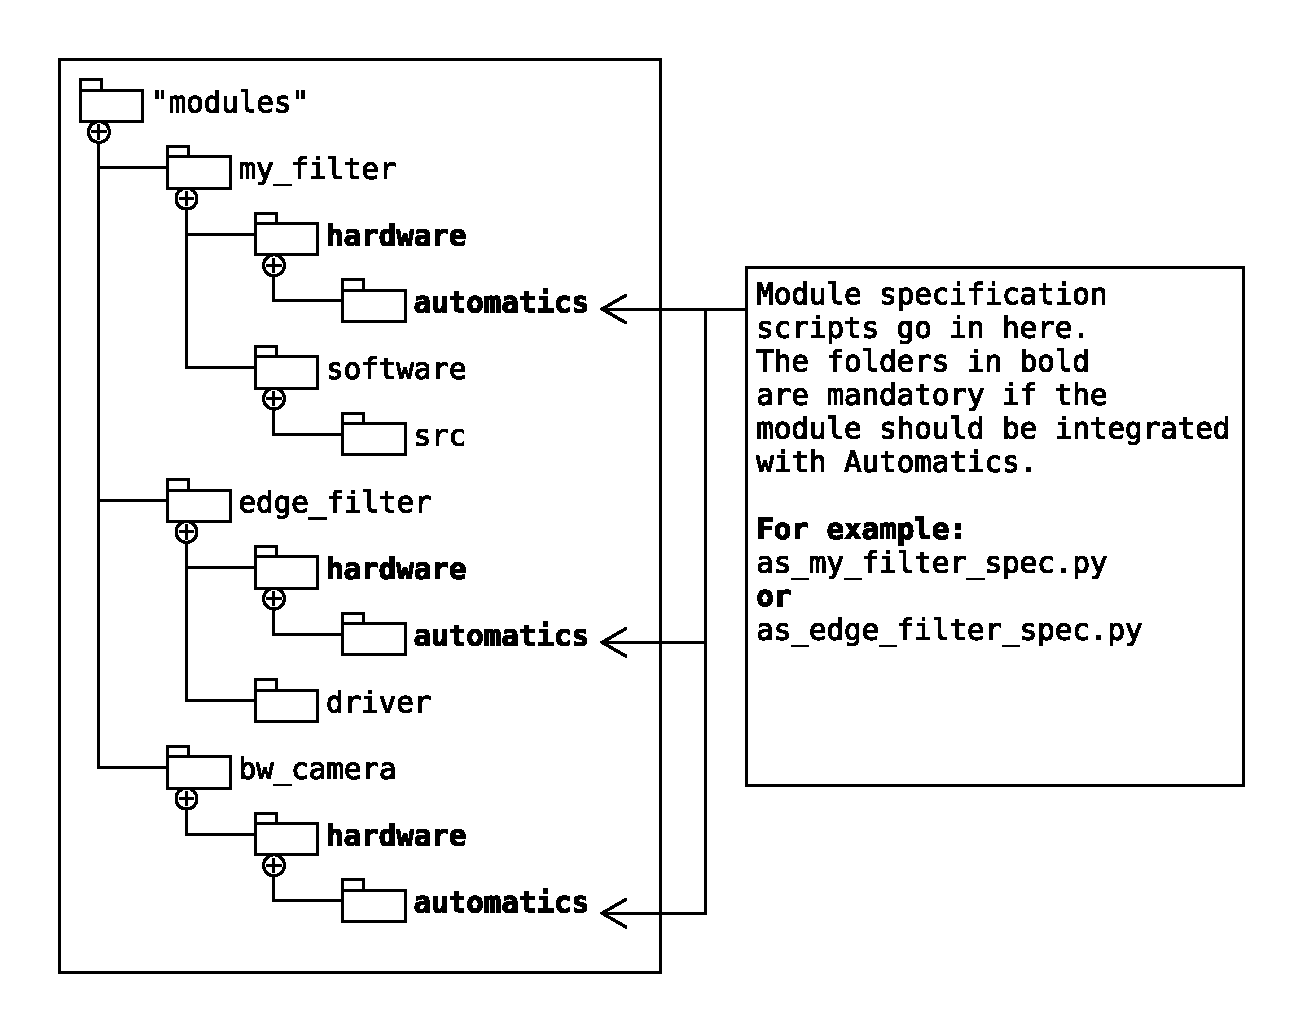
\includegraphics[width=0.9\textwidth]{./figs/06-02-Module_specification_folder_structure.eps}
\caption{Folder structure of source files of modules used with Automatics.}
\label{fig:06-02-module_folder_structure}
\end{figure}

As mentioned in section \ref{ssec:06-02-interface}, in the module specification files before the call to \lstapyinline{module.discover_module} new interface templates may be added to only this module by using the \lstapyinline{module.add_local_interface_template()} method.

Most other configuration options, such as modifying Ports, Generic and Interface settings, must be done after the call to \lstapyinline{module.discover_module()}, as this is the method Automatics uses to create all the Port, Generic and Interface objects.
Refer to the specification template file and the Doxygen documentation or the Python docstrings for explanations of the functionality of the available methods of the different Automatics objects.
Of main interest are the classes Port, Generic, Interface, AsModule, AsWindowModule, WindowInterface, Constant, AsRegisterInterface and AsModuleGroup.

To quickly get started with a custom module, one of the modules included with \asterics, contained in \texttt{asterics/modules} may be used as a starting point.

\subsubsection{Modules for Use in 2D Window Pipeline Systems - Window Modules}
\label{sec:06-02-custom_window_modules}

For modules that can be used in 2D Window Pipeline systems, certain special requisites must be fulfilled.
Firstly, to be correctly connected automatically, the module must be defined for Automatics, as an AsWindowModule Python class.
For this, a separate module specification script template is provided in the directory of all source files of Automatics (\lsthdlinline{asterics/tools/as-automatics/as_automatics_window_module_spec_template.py}).
Here is an example specification script of a window module (\texttt{as\_2d\_conv\_filter\_internal}):
\begin{lstlisting}[style=AutomaticsPython, label=lst:06-02_window_module_spec, caption=Specification script for a typical window module]
from as_automatics_2d_window_module import AsWindowModule

def get_module_instance(module_dir: str) -> AsWindowModule:

    module = AsWindowModule()
    toplevel_file = "hardware/hdl/vhdl/as_2d_conv_filter_internal.vhd"
    module.files = []
    module.dependencies = ["as_generic_filter_module"]
    module.processing_delay = 2

    # Automatics automatically parses the toplevel file and discovers
    # ports, generics, existing interfaces and register interfaces
    module.discover_module(module_dir + "/" + toplevel_file)

    return module
\end{lstlisting}

The only major differences to a regular specification script are first, instead of creating an AsModule object, an AsWindowModule object is created and, with that, all references to AsModule are replaced with AsWindowModule.
Secondly, the additional attribute \lstapyinline{processing\_delay} is set in line 9.
This attribute defines the processing delay in pixels for the module.
A processing delay of zero means that the result for an input is available in the same clock cycle as it was input into the module.
A processing delay of two means that two additional clock cycles are required by the module to process the value and that it will be available after two clock cycles on the modules output.
This value basically describes the number of register stages between the data input and output of the module.
Note that Automatics assumes that all outputs of a module have the same processing delay.
The default value for window modules is one.

Providing this additional meta data along with the same meta data as for a regular AsModule and instantiating it as an AsWindowModule are the only requisites to use a module in 2D Window Pipeline systems.\\

\emph{Note:} Modules declared as AsWindowModules are not usable in regular streaming type chains - only within an As2DWindowPipeline environment - as different connection rules apply. If you would like to use the same module in both contexts, you need to provide two separate specification scripts.
These must be analysed by Automatics either in two separate module repositories to differentiate between modules with identical entity names or point to two separate VHDL source files with different entity names.

\subsubsection{VHDL Coding Rules for \asterics Modules for Use with Automatics}
\label{sec:06-02-vhdl_quirks}

This section lists a few rules that must be followed in VHDL code for Automatics to correctly import a processing module.
These result from quirks of the VHDL Reader used in Automatics to parse the VHDL code.

\begin{itemize}
\item To end a VHDL \lsthdlinline{entity} either the entity name or the keyword \lsthdlinline{entity} must be used after the \lsthdlinline{end} keyword. Eg.: For \lsthdlinline{entity example is [...]} either \lsthdlinline{end example;}, \lsthdlinline{end entity;} or \lsthdlinline{end entity example;} must be used.
\item \lsthdlinline{port} and \lsthdlinline{generic} definitions in an \lsthdlinline{entity} must be in a single line.
\item The beginning and end of both \lsthdlinline{entity} and \lsthdlinline{architecture} must each be in a single line.
\item Port and generic names must not contain any of the following keywords: \lsthdlinline{entity, architecture} and \lsthdlinline{begin}.
\item Port and entity names should be kept all lower-case (within Automatics, they are handled and imported as all lower-case).
\item Generic names should be kept all upper-case (within Automatics, they are handled and imported as all upper-case).
\item The constant for the slave register configuration must be defined and contain the assignment operator (\lsthdlinline{:=}) in a single line. Further value assignments of the array may be spread out onto multiple lines.
\item Further, the constant must be placed before \emph{any} \lsthdlinline{begin} keyword, including \lsthdlinline{begin} as it appears in component, function or procedure declarations.
\end{itemize}

\emph{Note:} Automatics considers only the first entity in each VHDL file as an \asterics module.

All VHDL code after the \lsthdlinline{begin} statement in the \lsthdlinline{architecture} is ignored by Automatics.
No special considerations have to be followed for that code.

\subsubsection{VHDL Coding Rules for AsWindowModules}

For window inputs, VHDL ports that are the input for two dimensional matrices of pixels for filters, a special data type has to be used to facilitate automatic connection using Automatics:
\lsthdlinline{t_generic_window(0 to X, 0 to Y, bit width downto 0)}\\
A second type exists for working with lines of pixels of windows, which works in much the same way:
\lsthdlinline{t_generic_line(0 to X, bit width downto 0)}\\
These data types are specified in the \asterics VHDL package \texttt{as\_generic\_filter}, which must be included when using any of these types.

The range directions (to and downto) for these types \emph{must} be used as described here, as well as the each of the ranges defined meanings.\\

\lsthdlinline{t_generic_window} is the data type used to transfer 2D matrices of pixel data in a compact manner in \asterics.
The first dimension defines the width of the window, the X dimension.
The second dimension defines the height of the window, the Y dimension.
The third dimension defines the data width of the pixels in bits.
The following is an example definition of a 3 by 3 filter window for 8 bit data as a VHDL signal:
\lsthdlinline{signal window : t_generic_window(0 to 2, 0 to 2, 7 downto 0);}\\

\lsthdlinline{t_generic_line} is the data type used to handle single rows of pixel data (pixel arrays) in a manner compatible with \lsthdlinline{t_generic_window} in \asterics.
The first dimension defines the width of the line / row / array.
The second dimension defines the data width of the pixels in bits.
The following is an example definition of a line of 5 pixels with 9 bits each as a VHDL signal:
\lsthdlinline{signal line : t_generic_line(0 to 4, 8 downto 0);}\\

\lsthdlinline{t_integer_array} is a simple unbounded array of integers, used in the function \lsthdlinline{f_make_generic_window}.
It can be used to define fixed filter kernels for use in window modules and can be instantiated as in the following example:
\lsthdlinline{constant filter_values : t_integer_array(0 to 8) := (1,2,1,2,4,2,1,2,1);}\\
Alternatively, the type \lsthdlinline{t_generic_filter} may be used, which is a two dimensional integer array:\\
\lsthdlinline{constant filter_values : t_generic_filter(0 to 2, 0 to 2) := ((1,2,1),(2,4,2),(1,2,1));}



To make working with these data types easier, a number of helper functions are included in the package \texttt{as\_generic\_filter}.
The following is a brief list of all helper functions included for these special data types:
\begin{itemize}
\item \lsthdlinline{f_get_filter_sum_abs(gfilter)}: Calculate and return the absolute sum of all elements of \lsthdlinline{gfilter}.
\item \lsthdlinline{f_get_filter_max(gfilter)}: Find and return the largest value within \lsthdlinline{gfilter}.
\item \lsthdlinline{f_get_filter_elements_count(gfilter)}: Count and return the number of elements of \lsthdlinline{gfilter}.
\item \lsthdlinline{f_get_line_of_generic_filter(gfilter, y)}: Return a \lsthdlinline{t_integer_array} signal equal to the row at index \lsthdlinline{y} of \lsthdlinline{gfilter}.
\item \lsthdlinline{f_get_window_sum_abs(gwindow)}: Calculate and return the absolute sum of all elements of \lsthdlinline{gwindow}.
\item \lsthdlinline{f_get_vector_of_generic_window(gwindow, x, y)}: Extract and return the value of \lsthdlinline{gwindow} at the position (\lsthdlinline{x, y}) as a \lsthdlinline{std_logic_vector}.
\item \lsthdlinline{f_set_vector_of_generic_window(gwindow, x, y, vector)}: Set the value of \lsthdlinline{gwindow} at the position (\lsthdlinline{x, y}) to \lsthdlinline{vector}. Note: \lsthdlinline{vector} must have the same data width as the third dimension of \lsthdlinline{gwindow}!
\item \lsthdlinline{f_get_vector_of_generic_line(gline, x)}: Extract and return the value of \lsthdlinline{gline} at the position(\lsthdlinline{x}) as a \lsthdlinline{std_logic_vector}.
\item \lsthdlinline{f_set_vector_of_generic_line(gline, x, vector)}:  Set the value of \lsthdlinline{gline} at the position (\lsthdlinline{x}) to \lsthdlinline{vector}. Note: \lsthdlinline{vector} must have the same data width as the second dimension of \lsthdlinline{gline}!
\item \lsthdlinline{f_make_generic_window(x, y, values, data_width)}: Create and return a \lsthdlinline{t_generic_window} with the dimensions (\lsthdlinline{x, y, data_width}) and the contents of the \lsthdlinline{t_integer_array values}. Implemented for testing purposes but also useful for the definition of VHDL constants.
\item \lsthdlinline{f_get_line_of_generic_window(gwindow, y)}: Extract and return the row at position (\lsthdlinline{y}) of \lsthdlinline{gwindow} as a \lsthdlinline{t_generic_line} data type.
\item \lsthdlinline{f_set_line_of_generic_window(gwindow, y, line_in)}: Set the value of an entire or part of the row at position (\lsthdlinline{y}) of \lsthdlinline{gwindow} to the contents of \lsthdlinline{line_in}.
\item \lsthdlinline{f_get_part_line_of_generic_window(gwindow, y, from_x, width_part)}:  Extract and return part of the row at position (\lsthdlinline{y}) from position (\lsthdlinline{x}) and with a width of \lsthdlinline{width_part} data values from \lsthdlinline{gwindow} as a \lsthdlinline{t_generic_line} data type.
\item \lsthdlinline{f_cut_vectors_of_generic_line(gline, from_b, width_b)}: Return a \lsthdlinline{t_generic_line} signal based on part of the data of \lsthdlinline{gline} by cutting each data value from  bit \lsthdlinline{from_b} and only including the next \lsthdlinline{width_b} bits.
\item \lsthdlinline{f_cut_vectors_of_generic_window(gwindow, from_b, width_b)}: Return a \lsthdlinline{t_generic_window} signal based on part of the data of \lsthdlinline{gwindow} by cutting each data value from  bit \lsthdlinline{from_b} and only including the next \lsthdlinline{width_b} bits.
\end{itemize}

\subsubsection{Advanced Configuration of Custom Modules}
\label{sec:06-02-advanced_spec_scripts}

As every AsModule is at its core a Python object, they can be infinitely extended by adding methods and attributes in the specification script.
For example the module \texttt{as\_sensor\_ov7670} uses the specification script to add methods configuring the IIC masters that different modules in a system use.
For reference, the file can be found in \lsthdlinline{asterics/modules/as_sensor_ov7670/hardware/automatics/as_sensor_ov7670_spec.py}.
Note that this is an advanced configuration and should only be attempted if you are familiar with Python.
Attributes and methods configured as such will generally not be available in auto-completion features in IDEs and will not be listed for an AsModule when using the interactive modes of Automatics.


Furthermore, for a specific feature of Automatics, auto-instantiating modules, see the attribute \lstapyinline{instantiate_in_top} in section \ref{ssec:06-02-interface}, the method \lstapyinline{auto_inst_config} is defined as \lstapyinline{None} for every module.
It can be overwritten in the specification script to define actions to automatically take when the module is added to the system, as, at that point in the connection process, more information on the makeup of the system is available.
The method will always be passed the module instance itself and a reference to the module that instantiated it.
To see an example of this method being used, see the specification script of the \texttt{as\_regmgr} module in \lsthdlinline{asterics/modules/as_misc/hardware/automatics/as_regmgr_spec.py}.


\subsubsection{Adding a New Interface Template}
\label{sec:06-02-new_interface_template}

This section gives an overview of how interfaces are described in Automatics.

There are two types of interface templates in Automatics.
Both describe the general anatomy of an \lstapyinline{Interface} Automatics class, i.e. the types, directions and names of necessary and optional VHDL ports that comprise the interface.

\begin{itemize}
\item Global interface templates:
These templates are considered every time Automatics analyzes a new module.
This is potentially undesired, especially for interfaces consisting of very few and ports with potentially very generic names, as many false positives can be generated, i.e. interfaces are recognized, where ports are match by coincidence.
Templates are added to the list of global interface templates using the method \lstapyinline{asterics.add_global_interface_template()}.
These are disregarded when the modules that come with \asterics are imported.
Add your template to the file \texttt{as\_automatics\_templates.py} for the template to be considered for all modules imported.

\item Local interface templates:
These templates are only considered when importing a single module and must be added using the method \lstapyinline{module.add_local_interface_template()} within the module's specification script.
\end{itemize}

Each interface template is an abstraction of the Automatics Python class \lstapyinline{Interface}.
To define a new template, you may use the example provided below and modify it to match your interface.

\begin{lstlisting}[style=AutomaticsPython]
from as_automatics_interface import Interface
from as_automatics_port import Port

class AsStream(Interface):
    """Template definition for ASTERICS' 'as_stream' interface."""

    INTERFACE_TYPE_NAME = "as_stream"

    def __init__(self):
        super().__init__(self.INTERFACE_TYPE_NAME)
        self.add_port(Port("strobe"))
        self.add_port(Port("data", data_type="std_logic_vector"))
        self.add_port(Port("data_error", optional=True))
        self.add_port(Port("stall", direction="out", optional=True))
        self.add_port(Port("vsync", optional=True))
        vcomplete = Port("vcomplete", optional=True)
        vcomplete.add_rule("sink_missing", "fallback_port(vsync)", False)
        vcomplete.add_rule(
            "sink_missing", "fallback_port(data_unit_complete)", False
        )
        self.add_port(vcomplete)
        self.add_port(Port("hsync", optional=True))
        hcomplete = Port("hcomplete", optional=True)
        hcomplete.add_rule("sink_missing", "fallback_port(hsync)", False)
        self.add_port(hcomplete)
        self.add_port(Port("data_unit_complete", optional=True))

\end{lstlisting}

We recommend to put your interface templates into a separate file or, if it defined only for a single module, to add it into the specification file for that module.

To define a new template, you need use two classes of Automatics, \lstapyinline{Interface} and \lstapyinline{Port}, lines 1 and 2 import them from their respective Python files.

Line 4 declares a new Python class, in this case named \texttt{AsStream}, that inherits all attributes and functionality of the class \lstapyinline{Interface}.
You may name it (almost) anything you want, though we recommend the name of your interface in PascalCase.

Line 7 defines the name of the interface used by Automatics to refer to it.
Enter the name of your interface type here (must be unique).

Lines 9 and 10 initialize the template class and must be included without modifications.

All lines from line 11 on define the ports that comprise the interface.
You may use the example as guidance but should replace all lines from 11 to 26 with your own definitions.
In this section use the method \lstapyinline{self.add_port()} to add a \lstapyinline{Port} to the template.
Use the constructor \lstapyinline{Port()} to define new ports.

The following parameters can be used to define ports:

\begin{itemize}
\item \texttt{name=""}:
Define the main port name part expected by Automatics to recognize this port.
This means that even if prefixes or suffixes are added to the port name, it is still recognized.
For example: If a port is defined as \texttt{"data"}, Automatics will match the following port names to the port \texttt{"data\_1", "input\_data", "my\_data\_3", "data\_0\_additional"}.
Only if the name fragment \texttt{"data"} is not present, no match occurs.
This parameter must always be provided.
The parameter identifier (\texttt{name}) can be omitted, the first parameter is assumed to be the name of the port.

\item \texttt{direction=""}:
Data direction.
Equal to the VHDL data direction in the entity.
The possible values are: \texttt{"in", "out", "inout"}.
The default value is \texttt{"in"}.
\textit{Note:} The direction \texttt{"inout"} is only supported for external interfaces and ports, meaning interfaces and ports with no connections within the \asterics chain.

\item \texttt{data\_type=""}:
This parameter is equal to the VHDL data type.
No specific limitations exist.
The default value is \texttt{"std\_logic"}.
This parameter is purely treated as a string value and compared to the string extracted from the VHDL entity.

\item \texttt{optional=True/False}:
This boolean value defines whether the Port is necessary for the interface to be considered complete.
If any one port defined as not optional is missing in the entity of a module, that interface is not included in the module.
Inversely, any or all ports defined as optional may be missing in the entity and the interface will still be included.
The default value is \texttt{False}.
\end{itemize}

Furthermore, certain rules can be defined for each port.
To do this, assign a created \lstapyinline{Port} to a temporary variable, as seen with \texttt{vcomplete} in line 16 of the example above.
Now using the variable, the port can be further configured using methods regarding port rules.
A reference of port rule methods can be found in section \ref{sec:06-02-config_methods}.
After configuration, the port must be added to the template using the \lstapyinline{self.add_port()} method, as shown in line 21 of the example.

When using the methods \lstapyinline{asterics.add_global_interface_template()} and \lstapyinline{module.add_local_interface_template()} provide an instance of the template class, for example:
\begin{lstlisting}[style=AutomaticsPython]
# Global template
asterics.add_global_interface_template(AsStream())
# Local template (within module specification)
module.add_local_interface_template(AsStream())
\end{lstlisting}


\subsection{List of Methods for Use in Automatics Scripts}
\label{sec:06-02-config_methods}

This section lists configuration methods intended for use in Automatics scripts of Python classes of Automatics, to configure and build an \asterics processing chain.
All methods of the \lstapyinline{asterics} Python module, also used in Automatics scripts, are listed and detailed in section \ref{sec:06-02-cnns}.
The methods are listed in table \ref{tab:06-02-config_methods}.

A full account of all attributes, functions and methods available in Automatics and its classes can be found in the Doxygen documentation or directly in the source code.

\begin{longtable}[htbp]{|c|c|c|c|}
\hline 
\textbf{Object} & \textbf{Method} & \textbf{Parameters} & \textbf{Description} \\
\hline
\hline
\endhead
% ---------- AsProcessingChain --------------
\parbox{2.5cm}{~\\ \texttt{AsProcessing Chain}\\~} & \parbox{3cm}{~\\ \texttt{add\_module()}\\~} & \parbox{3cm}{~ \\ \texttt{entity\_name , user\_name, repo\_name} \\ ~} & \parbox{6cm}{~\\ Adds the module \texttt{entity\_name} from the module library to the processing chain. Optionally the module can be named using the \texttt{user\_name}, if ommitted, Automatics will enumerate using the \texttt{entity\_name}. Optionally, using the \texttt{repo\_name} a module can be chosen from a specific module repository. Useful to differentiate between modules with the same entity name imported from different repositories. \\~}\\
\hline
\parbox{2.5cm}{~\\ \texttt{AsProcessing Chain}\\~} & \parbox{3cm}{~\\ \texttt{set\_asterics\\\_base\_address()}\\~} & \parbox{3cm}{~ \\ \texttt{base\_address, address\_ space\_size} \\ ~} & \parbox{6cm}{~\\ Redefine the \asterics base address for communication between the \asterics modules and software. Set the available address space. \emph{Important:} Note that the base address must begin with all bits in the available space as zero. Eg.: OK: Base = \texttt{0x43C10000} and Size = \texttt{0xFFFF}, not OK: Base = \texttt{0x43C18000} and Size = \texttt{0x8FFF} (must be Base = \texttt{0x43C1{\color{blue}0}000}) \\~}\\
\hline
\parbox{2.5cm}{~\\ \texttt{AsProcessing Chain}\\~} & \parbox{3cm}{~\\ \texttt{connect()}\\~} & \parbox{3cm}{~ \\ \texttt{from, to} \\ ~} & \parbox{6cm}{~\\ Connect module, interface or port \texttt{from} to module, interface or port \texttt{to}. The direction of data flow is assumed to be from \texttt{from} to \texttt{to}, though an internal inspection will swap the objects if necessary. Note: The method call will be forwarded to the connect method of As2DWindowPipeline, if any object is part of a pipeline. \\~}\\
\hline
\parbox{2.5cm}{~\\ \texttt{AsProcessing Chain}\\~} & \parbox{3cm}{~\\ \texttt{write\_hw()}\\~} & \parbox{3cm}{~ \\ \texttt{folder, use\_symlinks, force} \\ ~} & \parbox{6cm}{~\\ Generate only the hardware source output files to \texttt{folder}. By default existing module source files are linked to the output folder. To copy them instead, use \lstapyinline{use_symlinks=False}. To allow Automatics to clean the output folder by permanently deleting contained files, set \lstapyinline{force=True}. \\~}\\
\hline
\parbox{2.5cm}{~\\ \texttt{AsProcessing Chain}\\~} & \parbox{3cm}{~\\ \texttt{write\_sw()}\\~} & \parbox{3cm}{~ \\ \texttt{folder, use\_symlinks, force, driver\_module\_\\\_dirs} \\ ~} & \parbox{6cm}{~\\ Generate only the software source output files to \textit{folder}. By default existing module source files are linked to the output folder. To copy them instead, use \lstapyinline{use_symlinks=False}.  To allow Automatics to clean the output folder by permanently deleting contained files, set \textit{force=True}. If you want source files sorted into subfolders per module, set \lstapyinline{driver_module_dirs=True}. \\~}\\
\hline
\parbox{2.5cm}{~\\ \texttt{AsProcessing Chain}\\~} & \parbox{3cm}{~\\ \texttt{write\_asterics\_\\ \_core()}\\~} & \parbox{3cm}{~ \\ \texttt{folder, use\_symlinks, force, driver\_module\_\\\_dirs} \\ ~} & \parbox{6cm}{~\\ Runs both \lstapyinline{write_hw()} and \lstapyinline{write_sw()}. The parameters are identical in functionality to those methods. \\~}\\
\hline
\parbox{2.5cm}{~\\ \texttt{AsProcessing Chain}\\~} & \parbox{3cm}{~\\ \texttt{write\_ip\_core\_\\ \_xilinx()}\\~} & \parbox{3cm}{~ \\ \texttt{folder, use\_symlinks, force, driver\_module\_ dirs} \\ ~} & \parbox{6cm}{~\\ Runs both \lstapyinline{write_hw()} and \lstapyinline{write_sw()}. The parameters are identical in functionality to those methods. In addition, the resulting IP-Core is packaged using Vivado. Vivado has to be installed on your system and sourced in the console environment you used to run Automatics for this step to complete. \\~}\\
\hline
\parbox{2.5cm}{~\\ \texttt{AsProcessing Chain}\\~} & \parbox{3cm}{~\\ \texttt{write\_system()}\\~} & \parbox{3cm}{~ \\ \texttt{folder, use\_symlinks, force, driver\_module\_\\\_dirs, add\_vears} \\ ~} & \parbox{6cm}{~\\ Runs both \lstapyinline{write_hw()} and \lstapyinline{write_sw()}. The parameters are identical in functionality to those methods.
The outputs are generated into a system template prepared for a Vivado-style FPGA project. In addition, the resulting IP-Core is packaged using Vivado. Vivado has to be installed on the system and sourced in the console environment used to run Automatics for this step to complete. Furthermore, the VEARS IP-Core for video output is added to the project. To omit it, set \lstapyinline{add_vears=False}. \\~}\\
\hline
\parbox{2.5cm}{~\\ \texttt{AsProcessing Chain}\\~} & \parbox{3cm}{~\\ \texttt{write\_system\_ graph()}\\~} & \parbox{3cm}{~ \\ \texttt{out\_file, show\_ toplevels, show\_auto\_ inst, show\_ports} \\ ~} & \parbox{6cm}{~\\ Generate and write a graph representation of the system represented by chain to the file \texttt{out\_file}. The other parameters are all \lstapyinline{False} by default and may be turned on (\lstapyinline{True}) to add detail. \texttt{show\_toplevels} adds "meta modules" used to connect  processing modules. \texttt{show\_auto\_inst} adds automatically instantiated modules. \texttt{show\_ports} adds a list of all ports to each edge of the graph which represent interfaces. \\~}\\
\hline
\parbox{2.5cm}{~\\ \texttt{AsProcessing Chain}\\~} & \parbox{3cm}{~\\ \texttt{list\_address \_space()}\\~} & \parbox{3cm}{~ \\ \texttt{None} \\ ~} & \parbox{6cm}{~\\ Call after building the processing chain to list the addresses and types of all allocated slave registers of the included modules. \\~}\\
\hline


% ---------- AsNNLayer --------------

\parbox{2.5cm}{~\\ \texttt{AsNNLayer}\\~} & \parbox{3cm}{~\\ \texttt{parametrize\_ and\_build()}\\~} & \parbox{3cm}{~ \\ \texttt{- omitted for brevity -} \\ ~} & \parbox{6cm}{~\\ Configure the neural network layer subsystem. The parameters are explained in section \ref{ssec:06-02-cnn_accel_module}.  \\~}\\
\hline

% ---------- As2DWindowPipeline --------------

\parbox{2.5cm}{~\\ \texttt{As2DWindow Pipeline}\\~} & \parbox{3cm}{~\\ \texttt{add\_module()}\\~} & \parbox{3cm}{~ \\ \texttt{entity\_name, user\_name, repo\_name} \\ ~} & \parbox{6cm}{~\\ Add a module to this As2DWindowPipeline with the entity name \texttt{entity\_name}. \emph{Only window modules} are considered when selecting the module. Optionally a name can be set for the module using \texttt{user\_name}. Optionally, using the \texttt{repo\_name} a module can be chosen from a specific module repository. Useful to differentiate between modules with the same entity name imported from different repositories.  \\~}\\
\hline
\parbox{2.5cm}{~\\ \texttt{As2DWindow Pipeline}\\~} & \parbox{3cm}{~\\ \texttt{connect()}\\~} & \parbox{3cm}{~ \\ \texttt{from, to, no\_delay, no\_stall} \\ ~} & \parbox{6cm}{~\\ Connect two objects, \texttt{from} and \texttt{to}, with each other within the pipeline. Additional optional parameters: \texttt{no\_delay}: if \texttt{from} is outside of the pipeline and this parameter is set to \lstapyinline{True}, no buffers to synchronize this input with all other input data will be created. \texttt{no\_stall}: if \texttt{to} is an \texttt{as\_stream} interface outside of the pipeline and \texttt{no\_stall} is set to \lstapyinline{True}, the \texttt{stall} signal of the target \texttt{as\_stream} interface will not be connected. Note: Calls to the processing chain's connect method with objects of a pipeline, will be forwarded to the pipeline's connect method, allowing for \lstapyinline{module0.connect(module1)} calls to connect modules of a pipeline.\\~}\\
\hline
\parbox{2.5cm}{~\\ \texttt{As2DWindow Pipeline}\\~} & \parbox{3cm}{~\\ \texttt{set\_flushing\_ behaviour()}\\~} & \parbox{3cm}{~ \\ \texttt{debug\_ flushdata, constant\_ flushdata\_ value} \\ ~} & \parbox{6cm}{~\\ Configure the behaviour of the flush control module included with every pipeline. Use \texttt{debug\_flushdata} to use a pixel counter as the flush data (\lstapyinline{True}) or a constant data word as flush data (\texttt{False}, default). Use \texttt{constant\_flushdata\_value} to define a custom value for the constant flush data. Default: 128. \\~}\\
\hline
\parbox{2.5cm}{~\\ \texttt{As2DWindow Pipeline}\\~} & \parbox{3cm}{~\\ \texttt{set\_main\_ buffer\_ optimization\_ strategy()}\\~} & \parbox{3cm}{~ \\ \texttt{new\_strategy} \\ ~} & \parbox{6cm}{~\\ Set the optimization strategy to use when optimizing the buffers of the window ports of the pipeline. Available optimizations are attributes of the pipeline object and prefixed with \lstapyinline{optimize\_}. Available options are: \lstapyinline{optimize\_none}, \lstapyinline{optimize\_row\_number\_sensitive}, \lstapyinline{optimize\_window\_width\_sensitive} and \lstapyinline{optimize\_all\_same\_length}; For a detailed explanation of the effects of each strategy, refer to section \ref{sec:06-02-2dpipe_general}\\~}\\
\hline
\parbox{2.5cm}{~\\ \texttt{As2DWindow Pipeline}\\~} & \parbox{3cm}{~\\ \texttt{set\_similar\_ length\_ optimization()}\\~} & \parbox{3cm}{~ \\ \texttt{active, max\_length\_ difference} \\ ~} & \parbox{6cm}{~\\ Configure the \textit{similar\_length} optimization step. Use \texttt{active} to turn the optimization on (\lstapyinline{True} (default)) and off (\lstapyinline{False}). Use \texttt{max\_length\_difference} to define the maximum length in pixels that buffers are merged. Higher numbers will result in less block-RAM tile usage but higher slice register usage (default: 100). \\~}\\
\hline
\parbox{2.5cm}{~\\ \texttt{As2DWindow Pipeline}\\~} & \parbox{3cm}{~\\ \texttt{set\_reshape\_ long\_buffers\_ optimization()}\\~} & \parbox{3cm}{~ \\ \texttt{active, minimum\_length \_to\_reshape, maximum\_width\_ to\_reshape} \\ ~} & \parbox{6cm}{~\\ Configure the \textit{reshape\_long\_buffers} optimization step. Use \texttt{active} to turn the optimization on (\lstapyinline{True} (default)) and off (\lstapyinline{False}). Use \texttt{minimum\_length\_to\_reshape} to define the minimum buffer length to be reshaped. With default value (-1) a value will be calculated from the pipeline's attribute \texttt{minimum\_bram\_size}. Use \texttt{maximum\_width\_to\_reshape} to define a maximum bit width of buffers to reshape. For additional details about the effects of this optimization, refer to section \ref{sec:06-02-2dpipe_general}. \\~}\\
\hline
\parbox{2.5cm}{~\\ \texttt{As2DWindow Pipeline}\\~} & \parbox{3cm}{~\\ \texttt{print\_pipeline\_ buffer\_report()}\\~} & \parbox{3cm}{~ \\ \texttt{verbosity} \\ ~} & \parbox{6cm}{~\\ Print a summary report of the buffer usage of the pipeline. Set \texttt{verbosity} to 1 to also print a report for every buffer. \\~}\\
\hline
% ---------- AsModuleGroup --------------

\parbox{2.5cm}{~\\ \texttt{AsModule Group} \\ and\\ \texttt{As2DWindow Pipeline}\\~} & \parbox{3cm}{~\\ \texttt{add\_register()}\\~} & \parbox{3cm}{~ \\ \texttt{register\_ type} \\ ~} & \parbox{6cm}{~\\ Create a 32 bit slave register for this module group. Use \texttt{register\_type} to define the type of register. Use \lstapyinline{asterics.Register.<type>} for the parameter. Possible types are \lstapyinline{none, control, status, both}. Refer to section \ref{sec:05-01-05-register_interface} for explanations on the different register types. \\~}\\
\hline
\parbox{2.5cm}{~\\ \texttt{AsModule Group} \\ and\\ \texttt{As2DWindow Pipeline}\\~} & \parbox{3cm}{~\\ \texttt{modify\_ register\_ type()}\\~} & \parbox{3cm}{~ \\ \texttt{register\_num, new\_type} \\ ~} & \parbox{6cm}{~\\ Modify the register type of the register with index \texttt{register\_num} to the type \texttt{new\_type}. For the value of \texttt{new\_type} use the same values as for the method \lstapyinline{add\_register} above. \\~}\\
\hline
\parbox{2.5cm}{~\\ \texttt{AsModule Group} \\ and\\ \texttt{As2DWindow Pipeline}\\~} & \parbox{3cm}{~\\ \texttt{assign\_ register\_ to\_port()}\\~} & \parbox{3cm}{~ \\ \texttt{register\_num, port, from\_bit\_ index} \\ ~} & \parbox{6cm}{~\\ Assign the value, or part of the value of a 32 bit slave register with index \texttt{register\_num} to the port or signal \texttt{port}. The port or signal will be assigned from the registers bit index \texttt{from\_bit\_index} up to the signals or ports bit width. The register will be automatically created if it doesn't exist. \\~}\\
\hline
\parbox{2.5cm}{~\\ \texttt{AsModule Group} \\ and\\ \texttt{As2DWindow Pipeline}\\~} & \parbox{3cm}{~\\ \texttt{assign\_port\_ to\_register()}\\~} & \parbox{3cm}{~ \\ \texttt{register\_num, port, to\_bit\_ index} \\ ~} & \parbox{6cm}{~\\ Assign the value of the port or signal \texttt{port} to a 32 bit slave register with index \texttt{register\_num}. The port or signals value will be assigned from the registers bit index \texttt{to\_bit\_index} up to the ports or signals bit width. The register will be automatically created if it doesn't exist. \\~}\\
\hline
\parbox{2.5cm}{~\\ \texttt{AsModule Group} \\ and\\ \texttt{As2DWindow Pipeline}\\~} & \parbox{3cm}{~\\ \texttt{define\_port()}\\~} & \parbox{3cm}{~ \\ \texttt{name, code\_name, direction, data\_type, data\_width, fixed\_value} \\ ~} & \parbox{6cm}{~\\ Create, add and return a new Port object for this module group. \texttt{name} defines the base name of the new Port. The optional \texttt{code\_name} defines the name of the port in VHDL, default is the value of \texttt{name}. The optional \texttt{direction} defines the data direction of the port. Valid values are \lstapyinline{"in"} (default), \lstapyinline{"out"} and \lstapyinline{"inout"} (only partial support for automatic connections). The optional \texttt{data\_type} defines the VHDL data type of the port. Default: \lsthdlinline{std\_logic}. The optional \texttt{"data\_width"} defines the data width for vector types. Use a Python tuple, e. g. \lstapyinline{(0, "to", 7)} or \lstapyinline{"DATA_WIDTH - 1", "downto", 0)}. Anything but single numbers must be passed as a string. The optional \texttt{fixed\_value} can be used to define a fixed value for the port as a string. Only useful for ports with direction \lstapyinline{"out"}. Note that ports with a fixed value have a limited support for connections, as they will be assigned the fixed value within the module group. \\~}\\
\hline
\parbox{2.5cm}{~\\ \texttt{AsModule Group} \\ and\\ \texttt{As2DWindow Pipeline}\\~} & \parbox{3cm}{~\\ \texttt{define\_signal()}\\~} & \parbox{3cm}{~ \\ \texttt{name, data\_type, data\_width, fixed\_value} \\ ~} & \parbox{6cm}{~\\ Create, add and return a new GenericSignal object for this module group. The parameters work analogous to the method \texttt{define\_port} above, with following exceptions: The \texttt{name} will always be used as the \texttt{code\_name} attribute of the signal. The \texttt{fixed\_value} is more useful as signals do not have a data direction and exist only within a module group. \\~}\\
\hline

% ---------- AsModule --------------

\parbox{2.5cm}{~\\ \texttt{AsModule}\\~} & \parbox{3cm}{~\\ \texttt{add\_software\_ driver\_file()}\\~} & \parbox{3cm}{~ \\ \texttt{path} \\ ~} & \parbox{6cm}{~\\ Add an additional software driver file to this module. The path may be relative from the execution location of the chain description script or absolute. \\~}\\
\hline
\parbox{2.5cm}{~\\ \texttt{AsModule}\\~} & \parbox{3cm}{~\\ \texttt{connect()}\\~} & \parbox{3cm}{~ \\ \texttt{object} \\ ~} & \parbox{6cm}{~\\ Shorthand for \lstapyinline{chain.connect(self, object)}. Can also be used for modules that are part of a 2D Window Pipeline. \\~}\\
\hline
\parbox{2.5cm}{~\\ \texttt{AsModule}\\~} & \parbox{3cm}{~\\ \texttt{get\_port()}\\~} & \parbox{3cm}{~ \\ \texttt{port\_name} \\ ~} & \parbox{6cm}{~\\ Return the Port of the module with the \texttt{code\_name} or \texttt{name} attribute \texttt{port name}. \\~}\\
\hline
\parbox{2.5cm}{~\\ \texttt{AsModule}\\~} & \parbox{3cm}{~\\ \texttt{get\_interface()}\\~} & \parbox{3cm}{~ \\ \texttt{interface\_name, direction, interface\_type} \\ ~} & \parbox{6cm}{~\\ Return the Interface of the module with the \texttt{name} and \texttt{pre-/suffix} attributes matching \texttt{interface\_name}. Optionally exclude any interfaces from the search not matching with \texttt{direction} and/or \texttt{interface\_type}. \\~}\\
\hline
\parbox{2.5cm}{~\\ \texttt{AsModule}\\~} & \parbox{3cm}{~\\ \texttt{get()}\\~} & \parbox{3cm}{~ \\ \texttt{name, direction} \\ ~} & \parbox{6cm}{~\\ Shorthand for a combination of \lstapyinline{get\_interface} and \lstapyinline{get\_port}. Returns the first interface matching \texttt{name} and \texttt{direction} or, if none was found, searches for a matching port instead.\\~}\\
\hline
\parbox{2.5cm}{~\\ \texttt{AsModule}\\~} & \parbox{3cm}{~\\ \texttt{get\_generic()}\\~} & \parbox{3cm}{~ \\ \texttt{generic\_name} \\ ~} & \parbox{6cm}{~\\ Return the Generic of the module with the \texttt{code\_name} or \texttt{name} attribute \texttt{generic\_name}. \\~}\\
\hline
\parbox{2.5cm}{~\\ \texttt{AsModule}\\~} & \parbox{3cm}{~\\ \texttt{make\_port \_external()}\\~} & \parbox{3cm}{~ \\ \texttt{port\_name, value} \\ ~} & \parbox{6cm}{~\\ Search for a Port matching \texttt{port\_name} and change it's \texttt{ruleset} to have Automatics make it external (default), meaning it will be available on the interface of the resulting IP-Core. Alternatively, make an external port internal by setting \texttt{value} to \lstapyinline{False}. \\~}\\
\hline
\parbox{2.5cm}{~\\ \texttt{AsModule}\\~} & \parbox{3cm}{~\\ \texttt{make\_interface \_external()}\\~} & \parbox{3cm}{~ \\ \texttt{interface\_name, direction, if\_type, value} \\ ~} & \parbox{6cm}{~\\ Search for an Interface matching \texttt{interface\_name} (and optionally \texttt{direction} and \texttt{if\_type}) to have Automatics make it external (default: \texttt{value} set to \lstapyinline{True}), meaning it will be available on the interface of the resulting IP-Core. Alternatively, make an external interface internal by setting \texttt{value} to \lstapyinline{False}. Note that you will have to either provide the parameter name (\lstapyinline{value=False}) or use all parameters. \\~}\\
\hline

\parbox{2.5cm}{~\\ \texttt{AsModule}\\~} & \parbox{3cm}{~\\ \texttt{set\_port \_fixed\_value()}\\~} & \parbox{3cm}{~ \\ \texttt{port\_name, value} \\ ~} & \parbox{6cm}{~\\ Search for a Port matching \texttt{port\_name} and change it's \texttt{ruleset} to have Automatics set it to the fixed value \texttt{value}. Automatics will directly insert the value of \texttt{value} into VHDL code, therefore it must adhere to VHDL syntax. \\~}\\
\hline
\parbox{2.5cm}{~\\ \texttt{AsModule}\\~} & \parbox{3cm}{~\\ \texttt{set\_generic \_value()}\\~} & \parbox{3cm}{~ \\ \texttt{generic\_name, value} \\ ~} & \parbox{6cm}{~\\ Search for a Generic of the module with the name \texttt{generic\_name} and set it's \texttt{value} attribute to the value of the parameter \texttt{value}. Note that the value of \texttt{value} will be directly inserted into VHDL code, therefore it must adhere to VHDL syntax. \\~}\\
\hline
\parbox{2.5cm}{~\\ \texttt{AsModule}\\~} & \parbox{3cm}{~\\ \texttt{port\_rule \_add()}\\~} & \parbox{3cm}{~ \\ \texttt{port\_name, condition, action, priority} \\ ~} & \parbox{6cm}{~\\ Search for a Port matching \texttt{port\_name} and add to it's \texttt{ruleset} the new rule \texttt{condition -> action}. This rule will have top priority, so will be executed first, unless the parameter \texttt{priority} is set to \lstapyinline{False}. \\~}\\
\hline
\parbox{2.5cm}{~\\ \texttt{AsModule}\\~} & \parbox{3cm}{~\\ \texttt{port\_rule \_remove()}\\~} & \parbox{3cm}{~ \\ \texttt{port\_name, condition, action} \\ ~} & \parbox{6cm}{~\\ Search for a Port matching \texttt{port\_name} and remove the rule \texttt{condition -> action} from it's \texttt{ruleset}, if it exists. \\~}\\
\hline
\parbox{2.5cm}{~\\ \texttt{AsModule}\\~} & \parbox{3cm}{~\\ \texttt{port\_rule \_overwrite()}\\~} & \parbox{3cm}{~ \\ \texttt{port\_name, condition, action} \\ ~} & \parbox{6cm}{~\\ Search for a Port matching \texttt{port\_name} and overwrite all \texttt{actions} for \texttt{condition} in it's \texttt{ruleset}. Then add the rule \texttt{condition -> action}. \\~}\\
\hline
\parbox{2.5cm}{~\\ \texttt{AsModule}\\~} & \parbox{3cm}{~\\ \texttt{make\_generic \_external()}\\~} & \parbox{3cm}{~ \\ \texttt{generic\_name} \\ ~} & \parbox{6cm}{~\\ For the Generic matching \texttt{generic\_name}, set its attributes so that it will be propagated to toplevel, allowing the synthesis tool to set the value using the \asterics IP-Core.\\~}\\
\hline

% ---------- Interface --------------
\parbox{2.5cm}{~\\ \texttt{Interface}\\~} & \parbox{3cm}{~\\ \texttt{connect()}\\~} & \parbox{3cm}{~ \\ \texttt{object} \\ ~} & \parbox{6cm}{~\\ Shorthand for \lstapyinline{chain.connect(self, object)}. Can also be used for interfaces that are part of modules within a 2D Window Pipeline. \\~}\\
\hline
\parbox{2.5cm}{~\\ \texttt{Interface}\\~} & \parbox{3cm}{~\\ \texttt{make\_external()}\\~} & \parbox{3cm}{~ \\ \texttt{value} \\ ~} & \parbox{6cm}{~\\ Set the necessary attribute to make this Interface available externally. Automatics will connect it to the VHDL toplevel, so it is in the interface of the resulting IP-Core. Set \texttt{value} to \lstapyinline{False} to make external interfaces internal. \\~}\\
\hline
\parbox{2.5cm}{~\\ \texttt{Interface}\\~} & \parbox{3cm}{~\\ \texttt{instantiate \_module()}\\~} & \parbox{3cm}{~ \\ \texttt{entity\_name, group\_name} \\ ~} & \parbox{6cm}{~\\ Set the necessary attributes to have Automatics automatically add and instantiate the \asterics module \texttt{entity\_name} and connect the interface to it. The \texttt{group\_name} defines where in the hardware design the module is instantiated. This particular functionality is currently not implemented completely - the only two options for the \texttt{group\_name} are: \lstapyinline{asterics}, to instantiate to the toplevel (default) and \lstapyinline{as_main} to instantiate the module where the \asterics modules are connected. This functionality is useful, for example, to instantiate necessary bus manager modules or similar. \\~}\\
\hline
\parbox{2.5cm}{~\\ \texttt{Interface}\\~} & \parbox{3cm}{~\\ \texttt{instantiate \_no\_module()}\\~} & \parbox{3cm}{~ \\ \texttt{None} \\ ~} & \parbox{6cm}{~\\ Remove a configuration for an automatic instantiation of a mode from this interface object. \\~}\\
\hline

% ---------- Generic --------------
\parbox{2.5cm}{~\\ \texttt{Generic}\\~} & \parbox{3cm}{~\\ \texttt{link\_to \_generic()}\\~} & \parbox{3cm}{~ \\ \texttt{link\_generic} \\ ~} & \parbox{6cm}{~\\ Set the necessary attributes to have Automatics link the value of this Generic to the Generic \texttt{link\_generic}, using the \texttt{code\_name} attribute, of higher modules. This can be useful, for example, to set the data bus width of multiple modules, using a user added Generic on the toplevel. (Note: This feature has not been tested extensively.) \\~}\\
\hline

% ---------- GenericSignal ----------

\parbox{2.5cm}{~\\ \texttt{Generic Signal}\\~} & \parbox{3cm}{~\\ \texttt{assign\_ from\_this\_ vector()}\\~} & \parbox{3cm}{~ \\ \texttt{target, from\_bit\_ index} \\ ~} & \parbox{6cm}{~\\ Partially assign from this signal. Only applicable for signals with a vector data type. Assign to port or signal \texttt{target} starting with bit index \texttt{from\_bit\_index} of the signal with the width of the target port or signal. \\~}\\
\hline
\parbox{2.5cm}{~\\ \texttt{Generic Signal}\\~} & \parbox{3cm}{~\\ \texttt{assign\_ to\_this\_ vector()}\\~} & \parbox{3cm}{~ \\ \texttt{source, from\_bit\_ index} \\ ~} & \parbox{6cm}{~\\ Assign the port or signal \texttt{source} to part of this signal. Only applicable for signals of a vector data type. Assign the source port or signal starting from bit index \texttt{from\_bit\_index} up to the data width of the source port or signal. \\~}\\
\hline
\parbox{2.5cm}{~\\ \texttt{Generic Signal}\\~} & \parbox{3cm}{~\\ \texttt{define\_ vector\_ assignment()}\\~} & \parbox{3cm}{~ \\ \texttt{source\_ list} \\ ~} & \parbox{6cm}{~\\ Define a list of source ports or signals \texttt{source\_list} to completely define the assignment of this signal. Only applicable for signals with a vector data type. The assignment starts at bit index zero and advances by the data width of each source port or signal in the list. The list keeps its order and will not be sorted. Equates to repeated calls to \lstapyinline{assign\_to\_this\_vector}. \\~}\\
\hline

% ---------- Port --------------
\parbox{2.5cm}{~\\ \texttt{Port} \\ and\\ \texttt{Generic Signal}\\~} & \parbox{3cm}{~\\ \texttt{connect()}\\~} & \parbox{3cm}{~ \\ \texttt{object} \\ ~} & \parbox{6cm}{~\\ Shorthand for \lstapyinline{chain.connect(self, object)}. Can also be used for ports that are part of modules within a 2D Window Pipeline. \\~}\\
\hline
\parbox{2.5cm}{~\\ \texttt{Port} \\ and\\ \texttt{Generic Signal}\\~} & \parbox{3cm}{~\\ \texttt{set\_port \_type()}\\~} & \parbox{3cm}{~ \\ \texttt{port type} \\ ~} & \parbox{6cm}{~\\ Manually define the Port's \texttt{port\_type} attribute. Useful if a Port is determined to have the wrong port type by Automatics. Valid values: \lstapyinline{"single"}, \lstapyinline{"external"}, \lstapyinline{"interface"}, \lstapyinline{"register"}, \lstapyinline{"signal"}, \lstapyinline{"glue\_signal"}. \\~}\\
\hline
\parbox{2.5cm}{~\\ \texttt{Port} \\ and\\ \texttt{Generic Signal}\\~} & \parbox{3cm}{~\\ \texttt{remove \_condition()}\\~} & \parbox{3cm}{~ \\ \texttt{condition} \\ ~} & \parbox{6cm}{~\\ Remove all rules with the condition \texttt{condition} from this Port's \texttt{ruleset}. You may use \lstapyinline{module.port_rule_overwrite}
\lstapyinline{(<port name>, <condition>, "none")} for the same effect. \\~}\\
\hline
\parbox{2.5cm}{~\\ \texttt{Port}\\ and\\ \texttt{Generic Signal}\\~} & \parbox{3cm}{~\\ \texttt{update \_ruleset()}\\~} & \parbox{3cm}{~ \\ \texttt{list} \\ ~} & \parbox{6cm}{~\\ Use this method to quickly add multiple rules to this Port's \texttt{ruleset}. Note that any invalid rules are quietly skipped. Any iterable list is accepted. Note that the rules are expected to use the \lstapyinline{Port.Rule namedtuple} (refer to the file \texttt{as\_automatics\_port.py}). \\~}\\
\hline
\parbox{2.5cm}{~\\ \texttt{Port} \\ and\\ \texttt{Generic Signal}\\~} & \parbox{3cm}{~\\ \texttt{set\_ruleset()}\\~} & \parbox{3cm}{~ \\ \texttt{list} \\ ~} & \parbox{6cm}{~\\ Use this method to quickly replace this Port's \texttt{ruleset}. Note that any invalid rules are quietly skipped. Any iterable list is accepted. Note that the rules are expected to use the \lstapyinline{Port.Rule namedtuple} (refer to the file \texttt{as\_automatics\_port.py}). \\~}\\
\hline

\parbox{2.5cm}{~\\ \texttt{Port} \\ and\\ \texttt{Generic Signal}\\~} & \parbox{3cm}{~\\ \texttt{add\_rule()}\\~} & \parbox{3cm}{~ \\ \texttt{rule\_condition}, \texttt{rule\_action}, \texttt{priority} \\ ~} & \parbox{6cm}{~\\ This method adds a Port rule condition, action pair. If the parameter \lstapyinline{priority} is set to \lstapyinline{True} (default) the new rule is inserted as the first rule to be applied when handling the port, giving it precedence over all prior rules. If \lstapyinline{priority} is set to  \lstapyinline{False} the new rule will be the last one to be applied. Refer to section \ref{ssec:06-02-class_port} for a full account of port rule conditions and actions. \\~}\\
\hline

\parbox{2.5cm}{~\\ \texttt{Port} \\ and\\ \texttt{Generic Signal}\\~} & \parbox{3cm}{~\\ \texttt{overwrite\_\\rule()}\\~} & \parbox{3cm}{~ \\ \texttt{rule\_condition}, \texttt{new\_action} \\ ~} & \parbox{6cm}{~\\ This method removes any rules using the condition \lstapyinline{rule_condition} and inserts the rule defined by \lstapyinline{rule_condition}, \lstapyinline{new_action}.
If no rules with \lstapyinline{rule_condition} exist, the new rule will not be inserted into the ruleset. \\~}\\
\hline

\parbox{2.5cm}{~\\ \texttt{Port} \\ and\\ \texttt{Generic Signal}\\~} & \parbox{3cm}{~\\ \texttt{remove\_rule()}\\~} & \parbox{3cm}{~ \\ \texttt{condition}, \texttt{action} \\ ~} & \parbox{6cm}{~\\ This method removes the first rule defined by both the specified \lstapyinline{condition} and \lstapyinline{action}. \\~}\\
\hline

\parbox{2.5cm}{~\\ \texttt{Port} \\ and\\ \texttt{Generic Signal}\\~} & \parbox{3cm}{~\\ \texttt{remove\_\\condition()}\\~} & \parbox{3cm}{~ \\ \texttt{rule\_condition} \\ ~} & \parbox{6cm}{~\\ This method removes all rules using the specified \lstapyinline{condition} from the port's ruleset. \\~}\\
\hline

\parbox{2.5cm}{~\\ \texttt{Port} \\ and\\ \texttt{Generic Signal}\\~} & \parbox{3cm}{~\\ \texttt{remove\_\\rule\_action()}\\~} & \parbox{3cm}{~ \\ \texttt{rule\_action} \\ ~} & \parbox{6cm}{~\\ This method removes all rules using the specified \lstapyinline{rule_action} from the port's ruleset. \\~}\\
\hline

\parbox{2.5cm}{~\\ \texttt{Port} \\~} & \parbox{3cm}{~\\ \texttt{make \_external()}\\~} & \parbox{3cm}{~ \\ \texttt{None} \\ ~} & \parbox{6cm}{~\\ Modify this Port's \texttt{ruleset} to have Automatics make it external. Same as AsModule's \lstapyinline{make_port_external()} method. \\~}\\
\hline

\caption{List of configuration methods intended for use in the user script.}
\label{tab:06-02-config_methods}
\end{longtable}






%%%%%%%%%%%%%%%%%%%%%%%%%%%%%%%%%%%%%%%%%%%%%%%%%%%%%%%%%%%%%%%%%%%%%%%%%%%%%%%
%%
%% This file is part of the ASTERICS Framework. 
%%
%% Copyright (C) Hochschule Augsburg, University of Applied Sciences
%% Efficient Embedded Systems Group
%%
%% Author(s): Gundolf Kiefer <gundolf.kiefer@hs-augsburg.de>
%%
%%%%%%%%%%%%%%%%%%%%%%%%%%%%%%%%%%%%%%%%%%%%%%%%%%%%%%%%%%%%%%%%%%%%%%%%%%%%%%


% TBD(PM): [GK 2018-07-09]
%   Diese Datei wird momentan nicht eigebunden. 
%   Hier könnte eine kurze Beschreibung des Estimator-Tools von 
%   Matthias Struwe hin (mit Verweis auf die Bachelorarbeit Struwe).
%
%   Vorher müsste das Estimator-Tool allerdings an den aktuellen
%   Stand des ASTERICS-Frameworks angepasst wird. Ob das passieren
%   wird oder im Rahmen der Projektarbeit von PM ein neues Tool
%   mit gleicher Funktionalität entsteht ist derzeit offen.


\section{The \asterics Chain Estimator} \label{ch:06-03-tools-estimator}




%%%%%%%%%%%%%%%%%%%%%%%%%%%%%%%%%%%%%%%%%%%%%%%%%%%%%%%%%%%%%%%%%%%%%%%%%%%%%%%
%%
%% This file is part of the ASTERICS Framework. 
%%
%% Copyright (C) Hochschule Augsburg, University of Applied Sciences
%% Efficient Embedded Systems Group
%%
%% Author(s): Gundolf Kiefer <gundolf.kiefer@hs-augsburg.de>
%%
%%%%%%%%%%%%%%%%%%%%%%%%%%%%%%%%%%%%%%%%%%%%%%%%%%%%%%%%%%%%%%%%%%%%%%%%%%%%%%



\section{2D Pipeline Generator} \label{ch:06-04-tools-pipegen}

\secauthor{Alexander Zöllner}

\subsection{Brief Description}
The \textit{2D Pipeline Generator} is a script-based tool for building a 2D pipeline in a semi-automatic way.
Required filter masks for the 2D window modules are extracted from images using the program Gimp.
The resulting 2D pipeline consists of storage elements for each data type and a number of \textit{2D Window Interfaces}.

Note: A similar functionality has been implemented into the Python script based generator Automatics, which will eventually supersede this generator tool.

\subsubsection{Hardware Components}

Table~\ref{06-04-pipeline-generator-components} lists the required hardware components for the 2D Pipeline Generator in order to build the pipeline.

\begin{longtable}[ht]{|c|c|}
\hline 
\textbf{Component} & \textbf{Purpose}\\
\hline 
\hline 
\endhead

\texttt{myLittleHelpersPkg.vhd} & 
\parbox{7cm}{ ~ \\ 
Defines several mathematic functions such as finding the exponent of two required for representing a given integer.
\\ ~ } \\

\hline 

\texttt{dram\_shift\_reg.vhd} & 
\parbox{7cm}{ ~ \\ 
Implements the logic required to store data in the 2D-sliding window buffer using distributed RAM (DRAM), i.e. slice registers. DRAM is used for small sections up to 100 elements.
\\ ~ } \\

\hline 

\texttt{bram\_shift\_reg.vhd} & 
\parbox{7cm}{~ \\ 
Implements the logic required to store data in the 2D-sliding window buffer using Block-RAM (BRAM). BRAM is used for long sections which require more than 100 elements.
\\ ~ } \\

\hline 

\texttt{myBRAM.vhd} & 
\parbox{7cm}{~ \\ 
Implements the actual storage element in BRAM.
\\ ~ } \\

\hline 

\caption{Hardware components required for the 2D Pipeline Generator} \label{06-04-pipeline-generator-components}\\
\end{longtable}

\subsubsection{Generator Input}
In order to build the 2D pipeline, the 2D Pipeline Generator has to determine the required interfaces.
Therefore, an image for each filter mask has to be provided using the image program Gimp (of version 2.8).
In the first step, a new image has to be created. 
The height of the image has to match the one of the filter mask and the width the resolution of the image in x direction.
For the filter mask, a new layer has to be created, matching the size of the image.
The layer should be named appropriately, since the generator uses the same name for the corresponding interface of the filter mask.
Further, the background layer has to be deleted.
The in- and output positions of the 2D window module are chosen by coloring the associated pixel, as shown in table~\ref{06-04-pipeline-generator-filter-masks}.
Reference pixels are solely for visual user assistance, e.g. marking the center pixel of a Gaussian filter mask.
In a final step, the generated image has to be exported in a png format.

\begin{longtable}[ht]{|c|c|c|c|}
  \hline
  & In & Ref. & Out \\
  \hline
  In & \cellcolor{red!75}0xff0000 & \cellcolor{yellow!75}0xffff00 & \cellcolor{magenta!75}0xff00ff \\
  \hline
  Ref. & \cellcolor{yellow!75}0xffff00 & \cellcolor{green!75}0x00ff00 & \cellcolor{cyan!25}0x00ffff \\
  \hline
  Out & \cellcolor{magenta!75}0xff00ff & \cellcolor{cyan!25}0x00ffff & \cellcolor{blue!75}0x0000ff \\
  \hline
  \caption{Color encoding used for I/O configuration} \label{06-04-pipeline-generator-filter-masks}
\end{longtable}

The in- and output ports of the filter masks have to be associated with their corresponding data type to infer the required amount of storage elements and connecting them correctly.
For this reason, an input file, namely \textit{data.txt} has to be provided, which contains labels for all data types with their associated bit width.
An entry has the format \texttt{<label>:<bit-width>}, where the \textit{label} must only contain letters (a-z, A-Z) and the \textit{bit-width} only digits (0-9).

Data types are associated with the filter masks by assigning the labels to the ports of a given filter port.
This is done in the \textit{connections.txt}, which is an output of the 2D Pipeline Generator.


\subsubsection{Scripts}

\begin{longtable}[ht]{|c|c|}
\hline 
\textbf{Name} & \textbf{Purpose} \\
\hline 
\hline 
\endhead

\texttt{generateConnectionFile.py} & 
\parbox{7cm}{ ~ \\ 
Generates the file connections.txt from the png files containing the filter masks and data.txt for the data types.
\\ ~ } \\

\hline 

\texttt{generateDataPipeline.py} & 
\parbox{7cm}{ ~ \\ 
Generates the actual 2D pipeline.
\\ ~ } \\

\hline 

\texttt{dataPipeline.py} & 
\parbox{7cm}{ ~ \\ 
Implements the functionality of the 2D Pipeline Generator and provides methods for generateConnectionFile.py and generateDataPipeline.py
\\ ~ } \\

\hline 

\caption{Scripts of the 2D Pipeline Generator} \label{06-04-pipeline-generator-scripts}\\
\end{longtable}

\subsection{Output Products}

\begin{longtable}[ht]{|c|c|}
\hline 
\textbf{Name} & \textbf{Purpose}\\
\hline 
\hline 
\endhead

\texttt{connections.txt} & 
\parbox{7cm}{ ~ \\ 
Lists ports of all filter masks. Has to be edited by user.
\\ ~ } \\

\hline 

\texttt{dataLayers.log} & 
\parbox{7cm}{ ~ \\ 
Lists the BRAM resource consumption as well as implementation details for individual layers.
\\ ~ } \\

\hline 

\texttt{dataPipeline.vhd} & 
\parbox{7cm}{~ \\ 
The vhdl module containing the 2D pipeline to be instantiated by the user.
\\ ~ } \\

\hline 

\texttt{dataPipeline\_mapping.vhd} & 
\parbox{7cm}{~ \\ 
Provides signal declarations and component instantiation in vhdl, which can be copied in the user design.
\\ ~ } \\

\hline 

\caption{Output products of the 2D Pipeline Generator} \label{06-04-pipeline-generator-output}\\
\end{longtable}
%%%%%%%%%%%%%%%%%%%%%%%%%%%%%%%%%%%%%%%%%%%%%%%%%%%%%%%%%%%%%%%%%%%%%%%%%%%%%%
%%
%% This file is part of the ASTERICS Framework. 
%%
%% (C) 2019 Hochschule Augsburg, University of Applied Sciences
%% Efficient Embedded Systems Group
%%
%% Author(s): Thibaut Temkeng <Thibaut.Temkeng@hs-augsburg.de>
%%
%%%%%%%%%%%%%%%%%%%%%%%%%%%%%%%%%%%%%%%%%%%%%%%%%%%%%%%%%%%%%%%%%%%%%%%%%%%%%%

	
\section{Graphical User Interface}\label{ch:06-05-tools-gui}

\secauthor{Thibaut Temkeng}

\infobox{The \asterics-GUI is still in development and not fully tested. See the application and this documentation as in-flux and experimental.}

This chapter introduces and describes the functionality of \asterics-GUI, the graphical user interface (GUI) of \asterics. The GUI is under constant development and its main goal is to speed up the learning curve for \asterics users, even if they have little programming knowledge. In other words, to make the use of the \asterics framework as easy as possible for the end user. The GUI offers the possibility to quickly become familiar with \asterics modules by listing all modules available in \asterics, providing module information such as port, generic, interface, dependencies, the path of the file describing the module, and how the module can be incorporated into an image processing chain. For more information on \asterics modules, see Section \ref{sec:06-05-modullist}. The GUI can also generate a complete functional image processing chain. For this purpose, a wizard is integrated into the GUI that guides the user step by step in the creation of an image processing chain as a Python script. The wizard can help you create your own image processing chain from scratch or create an image processing chain using a template that already exists in \asterics, see Section \ref{sec:06-05-wizard} for more information about the wizard.
	
	\subsubsection*{Prerequisites}
	\begin{itemize}
		\item An \asterics installation. See Section \ref{sec:02-installation}.
		\item Python 3.5 or a higher version.
		\item QT5, version \texttt{5.5} or higher
		\item Pandas. Installation using \textbf{pip install pandas}.
		\item The PyQt5 GUI library. Installation using \textbf{pip install pyqt5}.
	\end{itemize}

	\infobox{Note: On some Linux distributions installation of Python packages may require the use of the command \texttt{pip3} instead of \texttt{pip}. The package \texttt{pip[3]} may also need to be installed.}	
	
	\subsubsection*{Start the GUI}
	\begin{enumerate}
		\item Install the \asterics Framework (see chapter \ref{sec:02-installation}).
		\item Run the command line \texttt{"source settings.sh"} to source the \asterics settings file. The file \texttt{settings.sh} is located in the repository's root folder.
		\item Run the \texttt{"as-gui"} command to start the GUI and you should now have a window like the one shown in \ref{fig:GuiMainView}.
	\end{enumerate}

		\begin{figure}[!ht]
		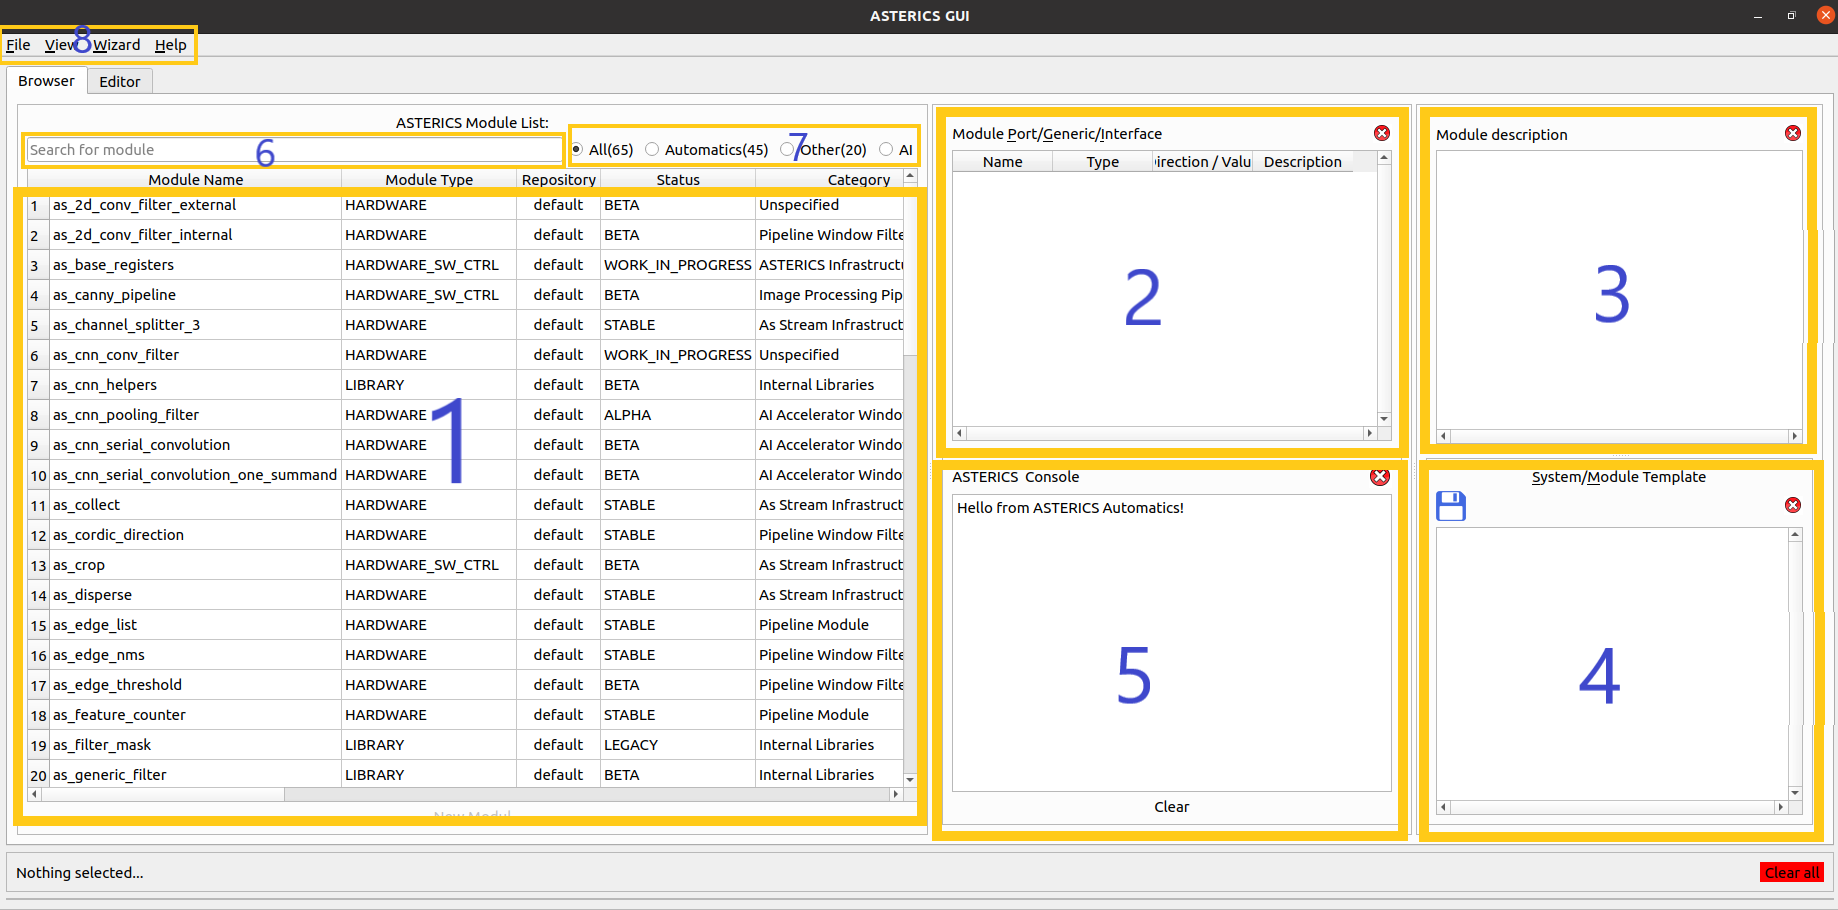
\includegraphics[width=\textwidth]{figs/gui/modulBrowser}
		\caption{GUI main view}
		\label{fig:GuiMainView}
	\end{figure}

	\subsection{Module Browser}
		\label{sec:06-05-modullist}
	This section explains how to use the \asterics-GUI to get details about the image processing modules available in \asterics.
	

	As it can be seen in the figure \ref{fig:GuiMainView}, the main GUI view is divided into smaller views with different goals. In the following, the different functionalities of these subviews will be described:
	\begin{enumerate}
		\item \textbf{Table of \asterics modules list}:\\
			Each row of this table describes an \asterics module and each row contains the following information:
		\begin{itemize}
			\item \lstcinline{Module Name}:\\
				The module name the same as the VHDL entity name.
			\item \lstcinline{Module type}: \\
				Each module has a type that is used to distinguish the modules that can process data e.g. only in hardware or only in software. In the table \ref{tab:06-05-module-type} all module types and the corresponding signification are listed:

			\begin{table}[!ht]
				\centering
				\footnotesize
				\begin{tabular}{|r|l|}
					\hline
					 \textbf{Module type} & \textbf{Signification} \\ \hline
					 UNSPECIFIED & No type specified \\ \hline
					 HARDWARE &Main \asterics hardware processing module \\ \hline
					 SOFTWARE &Main \asterics software processing module \\ \hline
					 LIBRARY& Library sub-module not fur use by the user (automatically inserted) \\ \hline
					 HARDWARE\_SOFTWARE &Main \asterics module processing both in software and hardware \\ \hline
					 HARDWARE\_SW\_CTRL& Main \asterics hardware processing module with a software driver \\ \hline
				\end{tabular}
				\caption{Module Type}
				\label{tab:06-05-module-type}
			\end{table}
			\item \lstcinline{Status}:\\
				From the beginning to the end of the implementation of a module, several steps are required, which are explained in the table \ref{tab:06-05-module-status}: 
		\begin{table}[!ht]
			\centering
			\footnotesize
			\begin{tabular}{|r|l|}
				\hline
				\textbf{Status} & \textbf{Signification} \\ \hline
				UNKNOWN& No state specified.\\ \hline
				 WORK\_IN\_PROGRESS &Code in development.\\ \hline
				 STABLE &In working condition and tested.\\ \hline
				 ALPHA &Code in development, some features work.\\ \hline
				 UNMAINTAINED& No longer maintained, not tested in current code base.\\ \hline
				 LEGACY& In working condition and maintained, but no longer up to date.\\ \hline
				 BETA &Code works, but not tested completely and not necessarily feature complete.\\ \hline
			\end{tabular}
			\caption{Module Status}
			\label{tab:06-05-module-status}
		\end{table}
		\item \lstcinline{Category}:\\
			The module category groups modules by their functionality.
		\item \lstcinline{Documentation}:\\It is currently under development. It is foreseen that this column contains a link that links the Doxygen documentation (to C, VHDL, or Python file) of the module.
		\item \lstcinline{Description}:\\ A rough description of the module.
		\end{itemize}
		\item \textbf{Module Port/Generic/Interface}:\\
			All ports, generics and interfaces of a module are listed here.
		\item \textbf{Modules Description }\\
		Here the module is described in more detail. We get additional information like on which modules the corresponding module depends and the path of the file that contains the implementation of the module.
		\item \textbf{System/Module Template}:\\
		In this view a generated Automatics script is displayed, which can then be saved locally with the button in the upper left corner.
		For something to be displayed in this view, there are two possibilities:
		\begin{enumerate}
			\item Click on a module from the first view.\\
			The generated script here is not a complete Automatics script, it only shows how the module should look like if it would be inserted into an image processing chain, no connection commands are generated.
			\item Click on the \texttt{"generate"} or \texttt{"Finish"} button from the wizard.\\
			The generated script is a complete and functional \automatics script and can therefore be used directly. In most cases, the generated script should be customized before use. 
		\end{enumerate}
		\item \textbf{\asterics Console}:\\
		This view shows the GUI history.
		\item \textbf{Search Bar}:\\
		The search bar facilitates the search for modules.  
		A module can be found by a part of the module name.  It is also useful that the part of the module's name does not have to match the beginning of the module name. For example, if the module \texttt{"as\_canny\_pipeline\_ent"} is searched, the keywords such as \texttt{"can"}, \texttt{"pip"}, \texttt{"ent"} etc can be used to search. Modules can also be searched by category, status or module type. Using the search word \texttt{"BETA"} will only list modules that have the status \texttt{"BETA"}.
		\item \textbf{Filter}:\\
		Not all \asterics modules can be directly introduced into an image processing chain, because they are e.g only sub- or auxiliary modules or also because \automatics cannot automatically include all modules into an image processing chain. With the option button \texttt{"All"} all \asterics modules are displayed, with \texttt{"Automatics"} all modules are listed which \automatics can automatically integrate into an image processing chain and with \texttt{"Other"} all modules not supported by \automatics are listed.
		\item \textbf{Menu Bar}:\\
			The menu bar offers the possibility to control the GUI more easily. The functionality of each menu are described in the following
			\begin{itemize}
				\item \textbf{File}:\\This menu provides two actions:
					\begin{enumerate}
						\item \lstapyinline{Exit}: Close the GUI. The key combination \textit{Ctrl+W} can be used to trigger this action.
						\item \lstapyinline{Add Repository}: It is currently under development. This should allow adding a folder as a new repository to the module library and adding all new modules to the module list. The key combination \textit{Ctrl+N} can be used to trigger this action.
					\end{enumerate}
				\item \textbf{View}: \\This menu provides five actions:
					\begin{enumerate}
						\item \lstapyinline{Template}: This action hides or shows the \textit{System/Module Template} view.
						\item \lstapyinline{Console}: This action hides or shows the \textit{Console} view.
						\item \lstapyinline{Port/Generic/Interface}: This action hides or shows  the \textit{Port/Generic/Interface} view.
						\item \lstapyinline{Modules Description}: This action hides or shows  the \textit{Module Description} view.
						\item \lstcinline{Restore all Views}: This action can be used to restore all views if they were previously closed.
					\end{enumerate}
				\item \textbf{Wizard}:\\This menu provides two actions:
					\begin{enumerate}
						\item \lstcinline{Start}: Start the Wizard. The key combination \textit{Ctrl+O} can be used to trigger this action.
						\item \lstcinline{Close}: Close the Wizard.
					\end{enumerate}
				\item \textbf{Help}: \\It is currently under development. It will allow you get information about \asterics such as the link to the Doxygen documentation of C, VHDL and Python files, new features to come,the contact of people who can help you in case of problems with \asterics and even more.
			\end{itemize}

	\end{enumerate}
	\subsection{Wizard}\label{sec:06-05-wizard}
	This section deals with ways to quickly create simple linear image processing chains. By linear it is meant that all modules in the chain excluding the input and output module get a single input and give a single output.
	There are two ways to create an image processing chain: either build the image processing chain from scratch (see Section \ref{subsub:06-05-new-system}), or use a template available in \asterics as a basis (see Section \ref{subsub:06-05-new-system-based-on-template}).
	To start the wizard, you should press the \texttt{"systems"} button in the 8th view (see the \ref{fig:GuiMainView} figure). A window like in \ref{fig:wizard} should appear. Now you can simply follow the instructions to create your image processing chain.
	\begin{figure}[!ht]
		\centering
		\begin{minipage}{0.45\textwidth}
			\centering
			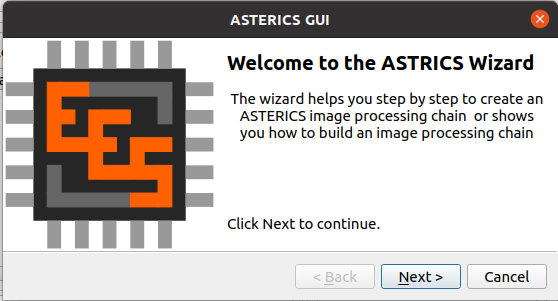
\includegraphics[width=\textwidth]{figs/gui/wizard}
			\caption{Wizard start window}
			\label{fig:wizard}
		\end{minipage} 
		\hfill
		\begin{minipage}{0.45\textwidth}
			\centering
			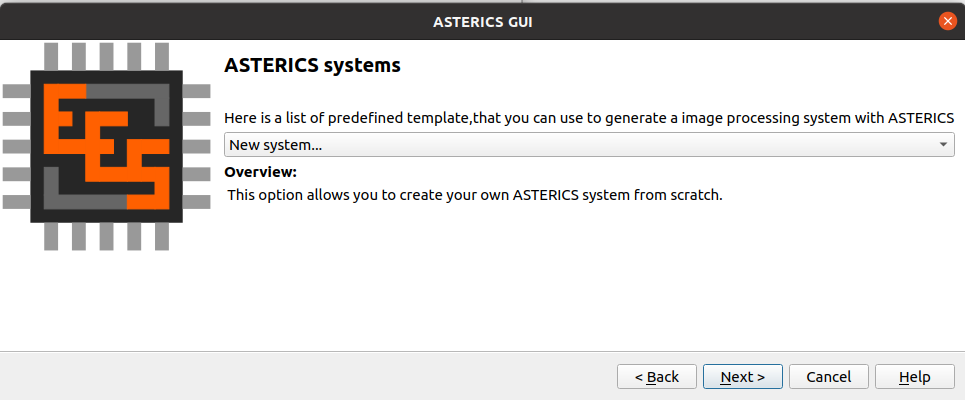
\includegraphics[width=\textwidth,]{figs/gui/list}
			\caption{List of \asterics Systems}

			\label{fig:astericsList}
		\end{minipage}
		
		
	\end{figure}
	\subsubsection{Generate a new System from scratch}\label{subsub:06-05-new-system}
	This section explains how to use the wizard to create a new image processing chain from scratch.
	Exactly how the creation proceeds is shown in the figure \ref{fig:06-05-wizard_input} to \ref{fig:06-05-wizard_connexion} and described in the following steps.
	\begin{figure}[!ht]
		\centering
		\begin{minipage}{0.45\textwidth}
			\centering
			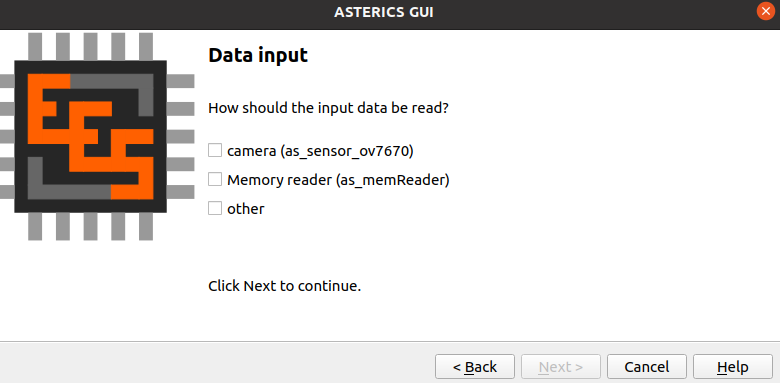
\includegraphics[width=\textwidth]{figs/gui/datainput}
			\caption{Input source}
			\label{fig:06-05-wizard_input}
		\end{minipage} 
		\hfill
		\begin{minipage}{0.45\textwidth}
			\centering
			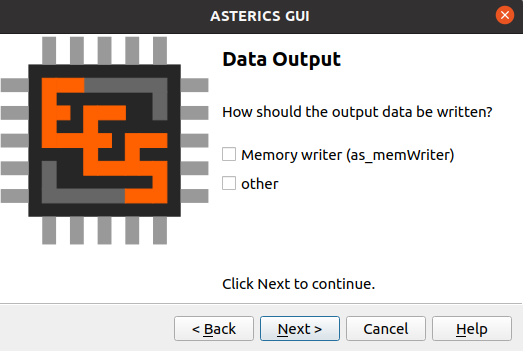
\includegraphics[width=\textwidth,]{figs/gui/dataoutput}
			\caption{Output source}
			\label{fig:06-05-wizard_output}
		\end{minipage}
		\begin{minipage}{0.45\textwidth}
			\centering
			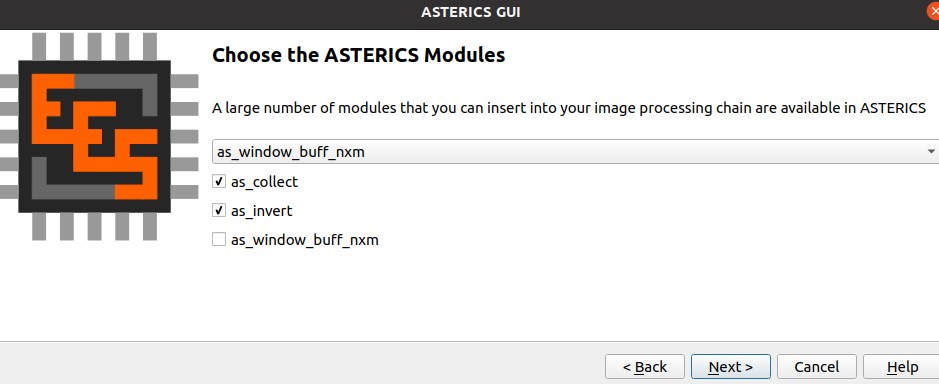
\includegraphics[width=\textwidth]{figs/gui/choose}
			\caption{Choose moduls}
			\label{fig:06-05-wizard_choose}
		\end{minipage} 
		\hfill
		\begin{minipage}{0.45\textwidth}
			\centering
			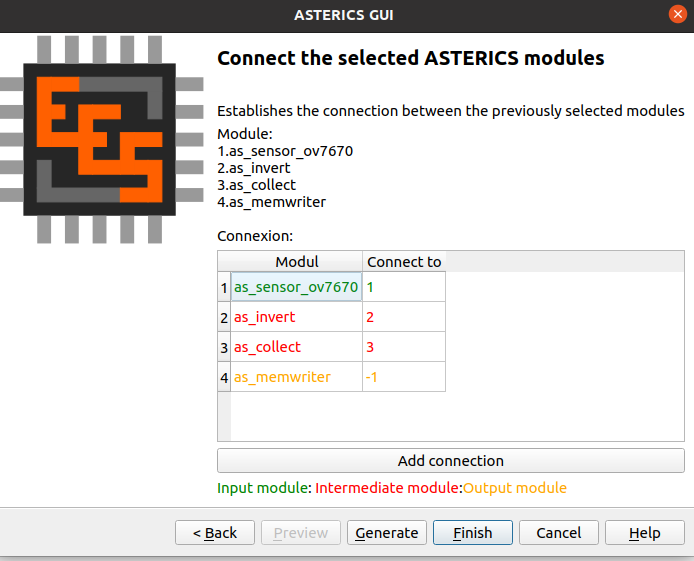
\includegraphics[width=\textwidth,]{figs/gui/connection}
			\caption{Connect moduls}
			\label{fig:06-05-wizard_connexion}
		\end{minipage}
	\end{figure}
	
	\begin{enumerate}
		\item Figure \ref{fig:06-05-wizard_input}: Choose how the input to the image processing chain is to be read. The input can be read directly from the camera, which corresponds to the \texttt{camera(as\_sensor\_ov7670)} option, or read from a file (image or video) from the hard disk, which corresponds to the \texttt{Memory reader (as\_memReader)} option. The latter option \texttt{other} is currently under development and intended for other input sources like USB stick.
		
		\item Figure \ref{fig:06-05-wizard_output}: After the input source has been selected, it should now be selected how the processed input should be written. With the option \texttt{Memory writer (as\_memWriter)} the output is written to memory and the option \texttt{other} is currently under development.
		
		\item Figure \ref{fig:06-05-wizard_choose}: The modules that are to process the input are selected from the list. It must be considered that not all \asterics modules are listed here because Automatics cannot automatically include all modules in an image processing chain or because they have already been used as input modules or output modules. If a selected module is not to be used any more, it must be simply checked off and is not considered in further.
		
		\item Figure \ref{fig:06-05-wizard_connexion}: Now the selected \asterics modules should be connected. In this view, all modules involved in the image processing chain are listed, and then how these modules are connected is shown in a table. In green is the input module (currently only one input module can exist in the chain, so it cannot read data from different input sources into one chain), in red are the intermediate modules (modules that process the input), and in yellow is the output module. The connection between two modules is shown in the column \texttt{"connect to"}. The first row in the table from the figure \ref{fig:06-05-wizard_connexion} means that the input module \texttt{as\_sensor\_ov7670} is directly connected to the module \texttt{as\_invert}. The number in the column  \texttt{"connect to"} must always be added by one to find the corresponding module or row from the table. The number in the \texttt{"connect to"} column are not fixed and can be adjusted. -1 means that the output of the module will not be processed further, the -1 is intended for the output module.  To generate the system, click on the button \texttt{"Generate"} or \texttt{"Finish"}. The generated script is located in the 4th view of the figure \ref{fig:GuiMainView} and can then be customized and saved.See Section \ref{subsub:06-05-generated-script} for further processing of the generated script 
	\end{enumerate}
	\subsubsection{Generate a new System based on Template}\label{subsub:06-05-new-system-based-on-template}
	This section explains how to use the Wizard to create a new computer vision system based on a template available in \asterics. The \asterics framework provides demonstration systems to facilitate familiarization with the concepts of the framework and its modules. The demo systems are already functional and can be used as a template for creating other systems.
	\begin{figure}[!ht]
		\centering
		\begin{minipage}{0.47\textwidth}
			\centering
			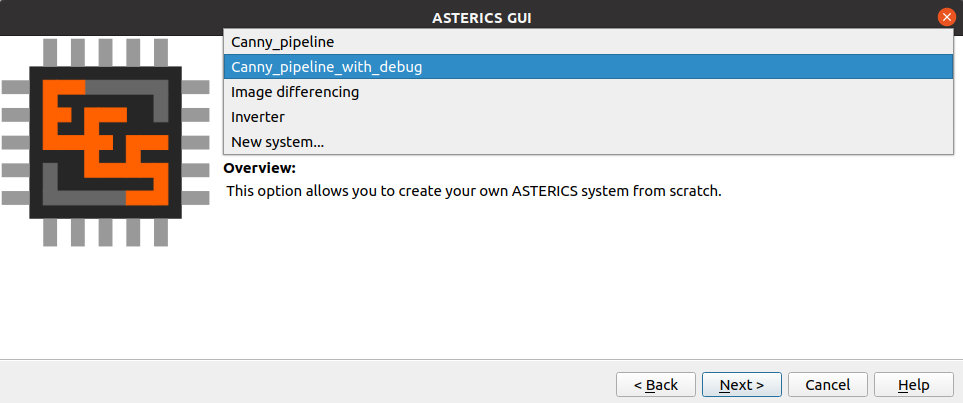
\includegraphics[width=\textwidth]{figs/gui/box}
			\caption{List on existing template}
			\label{fig:box}
		\end{minipage} 
		\hfill
		\begin{minipage}{0.47\textwidth}
			\centering
			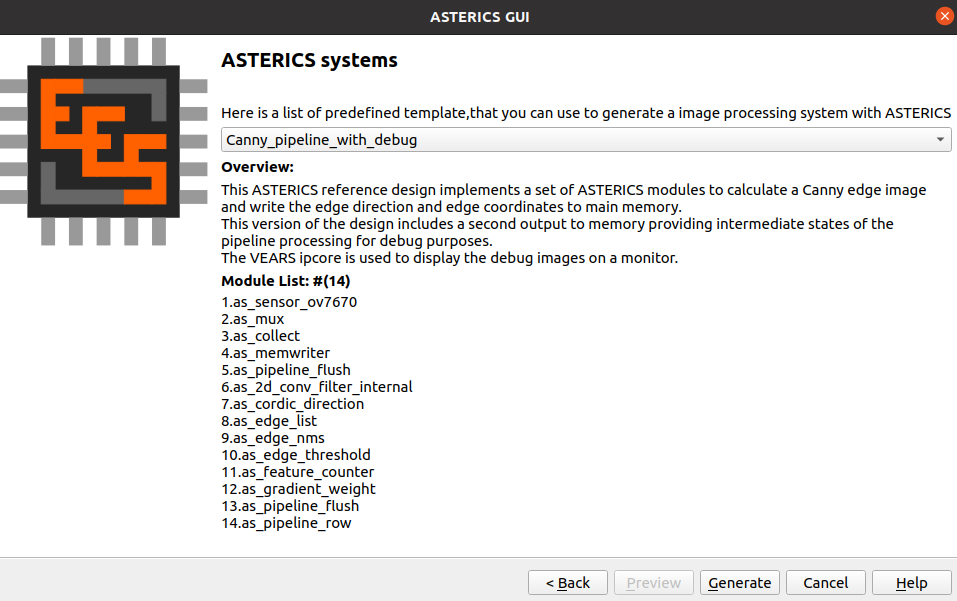
\includegraphics[width=\textwidth,]{figs/gui/exist}
			\caption{Description of an existing module}
			\label{fig:exist}
		\end{minipage}
	\end{figure}
	Compared to creating image processing systems from scratch, generating systems with template is faster. As it is shown in the figure \ref{fig:box}, there are already a few templates in \asterics. When a template is selected, a rough overview of the template's system is displayed, followed by a list of all modules involved in the chain. The system can then be created by clicking on the button \texttt{"Generate"}(see figure \ref{fig:exist}).
	
	\subsubsection{Use the generated Script}\label{subsub:06-05-generated-script}
	This section explains how to use the generated script.The generated script is located in the 4th view of Figure \ref{fig:GuiMainView} after clicking the "Generate" or "Finish" button of the wizard.  
	To save the script, you should click on the icon of the 4th view, which is the "Save As" button. You can manually customize the generated script again in your favorite editor after saving it. The script must be saved as Python file. Depending on whether the script was created from scratch or came from a demo system, the script will look different, especially when selecting the output products. Assuming that the script is saved under the name \texttt{"asterics-gen.py"}:
\begin{lstlisting}[style=AutomaticsPython, label=Code:06-05-demo-output-product, caption=Script: Demo system output product]

############### Automatics outputs ##############################

if len(sys.argv) < 3:
	print(
	(
		"Not enough parameters!\n"
		"Usage:\nasterics-gen.py build-target output-folder\n"
		"Valid build-targets: 'vivado', 'core'"
	)
 )
sys.exit()

# Build chain: Generate output products
# Write the outputs for the ASTERICS core

# Stores wether Automatics completed without errors or not
success = False

if sys.argv[1] == "vivado":
	success = chain.write_ip_core_xilinx(
	sys.argv[2] + "/ASTERICS", use_symlinks=True, force=True
	)
if success:
	# Create link to the VEARS IP-Core
	success = asterics.vears(sys.argv[2], use_symlinks=True, force=True)
elif sys.argv[1] == "core":
	success = chain.write_asterics_core(sys.argv[2], use_symlinks=True)
else:
	sys.exit("Not a valid build target!")
# On success, generate a system graph using dot
if success:
	chain.write_system_graph("asterics_system_graph")

# Report
if success:
	print("Automatics completed successfully!")
else:
	print("Automatics encountered errors:")
	asterics.list_errors()
\end{lstlisting}
	\begin{itemize}
		\item \textbf{Demo systems:}\\
			The script part representing the output products looks like in Listing \ref{Code:06-05-demo-output-product}. You can generate the output products using the following command line:
\begin{lstlisting}[style=shell]
$ python asterics-gen.py build-target output-folder
\end{lstlisting}
or 
\begin{lstlisting}[style=shell]
$ python3 asterics-gen.py build-target output-folder
\end{lstlisting}
			Where \textit{build-target} must be either \texttt{"vivado"} or \texttt{"core"}. With \texttt{"vivado"}, the \asterics system generator \automatics generates the source file for the described \asterics chain and packages them to an IP-Core using Xilinx Vivado. With \texttt{"core"}, \automatics generates only the \asterics chain source files to the the folder \textit{output-folder}. \textit{output-folder} is the name of the directory where the output products must be stored. For more information about the output product see \ref{ssec:02-output}.
		\item \textbf{Your own system:} \\
			For the systems you have built yourself, the script part representing the output products looks like in Listing \ref{Code:06-05-system-from-scratch-output-product}. All possible output products are listed. Depending on your application, you can generate only the necessary products. You only have to adjust the output folder \texttt{"destination\_dir"} and the path \texttt{"output\_file"} and then the script can be generated. After saving the generated script, run the command line to generate the output products:
\begin{lstlisting}[style=shell]
 $	python(3) asterics-gen.py
\end{lstlisting}
			
	\end{itemize}


\begin{lstlisting}[style=AutomaticsPython, label=Code:06-05-system-from-scratch-output-product, caption=Script: Output product of systems created with the wizard from scratch]
# Automatics output products 
# All possible output products are listed below and it is 
#			not necessary to generate all of them.
# vivado
chain.write_ip_core_xilinx(path='destination_dir', use_symlinks=True, 
							force=False, module_driver_dirs=False)
# Create link to the VEARS IP-Core
asterics.vears(path='destination_dir', use_symlinks=True, force=False)
# Core
chain.write_asterics_core(path='destination_dir', use_symlinks=True, 
							force=False, module_driver_dirs=False)
# System
chain.write_system(path='destination_dir', use_symlinks=True, 
	force=False, module_driver_dirs=False, add_vears=False)
# SVG graph
chain.write_system_graph(out_file='output_file', show_toplevels=False, 
						show_auto_inst=False, show_ports=False, 
						show_unconnected=False, show_line_buffers=False)
\end{lstlisting}
\begin{figure}[h]
	\centering
	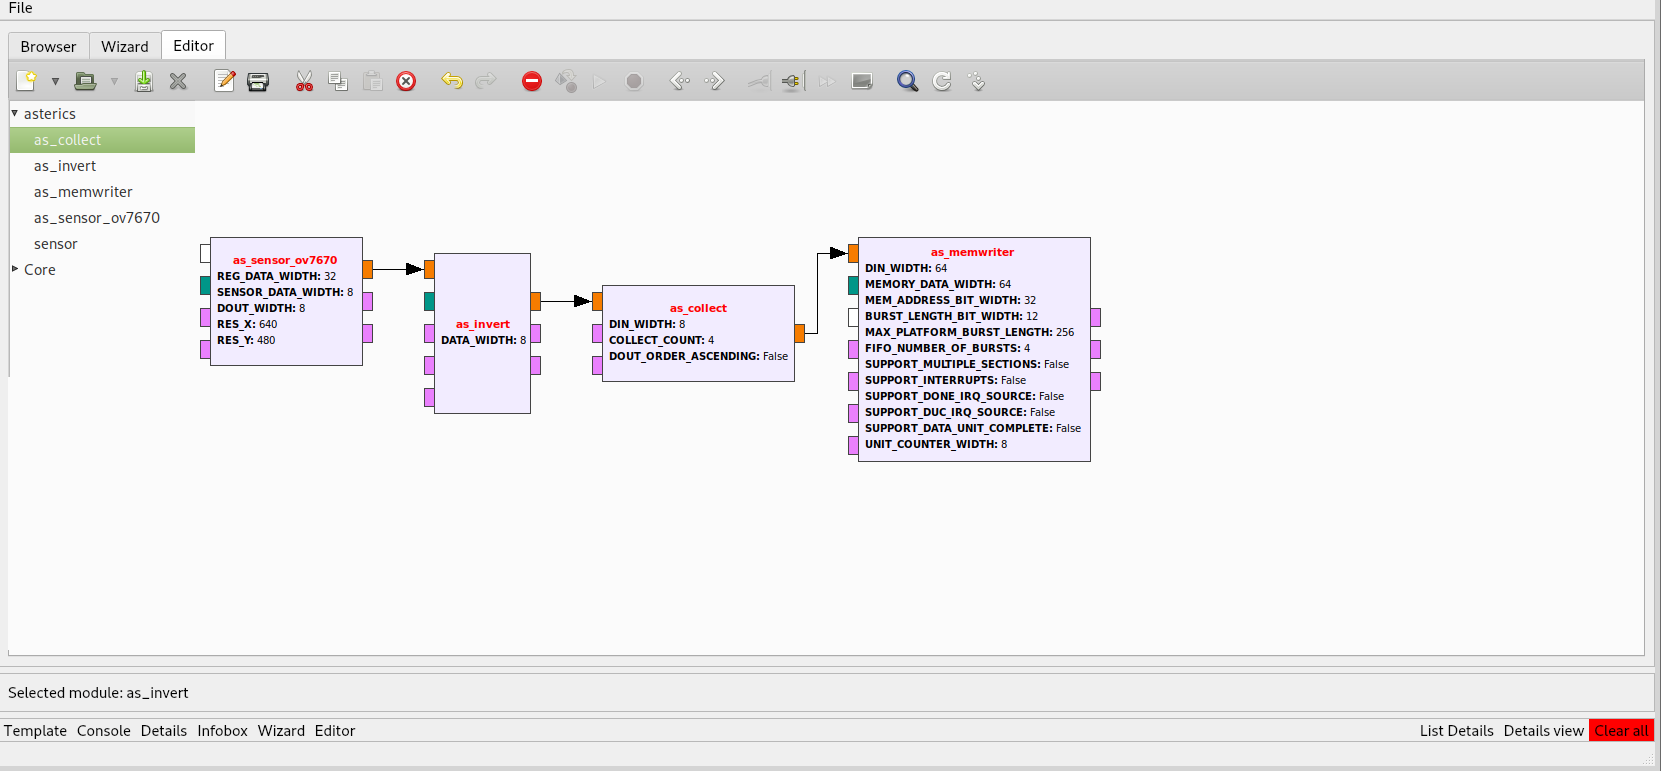
\includegraphics[width=\textwidth]{figs/gui/editor}
	\caption{Inverter system with editor.}
	\label{fig:editor}
\end{figure}
	\subsection{Editor}\label{sec:06-05-editor}
		The editor is currently under development and it should make the creation of image processing chains even easier and faster. It should not only be possible to create simple image processing chains, but also complex ones and the representation of systems should also be possible graphically. Figure \ref{fig:editor} shows an inverter system with the current version of the editor.
	\newpage	
		
		


%%%%%%%%%%%%%%%%%%%%%%%%%%%%%%%%%%%%%%%%%%%%%%%%%%%%%%%%%%%%%%%%%%%%%%%%%%%%%%
%%
%% This file is part of the ASTERICS Framework. 
%%
%% (C) 2021 Hochschule Augsburg, University of Applied Sciences
%% Efficient Embedded Systems Group
%%
%% Author(s): Gundolf Kiefer <gundolf.kiefer@hs-augsburg.de>
%%            Philip Manke <philip.manke@hs-augsburg.de>
%%
%%%%%%%%%%%%%%%%%%%%%%%%%%%%%%%%%%%%%%%%%%%%%%%%%%%%%%%%%%%%%%%%%%%%%%%%%%%%%%





%%%%%%%%%%%%%%%%%%%%%%%%%%%%% 7. Modules %%%%%%%%%%%%%%%%%%%%%%%%%%%%%%%%%%%%%

%% NOTE: Only modules from the public ASTERICS are documented here.
%%       Please add documentation for the 'asterics-nonfree' and 
%%       project-specific repos to '07int-modules.tex'!


\chapter{Basic Modules} \label{ch:07-modules}

The \asterics framework includes a multitude of processing and infrastructure modules.
This chapter serves as the documentation of the functionality and user reference for the simpler \asterics modules.


%\begin{verbatim}
%[[
%
%TBD (MS/JS/alle):
%
%Für jedes existierende Modul ein Datenblatt 
%- Umfang 1/2 - 1 Seite (komplexe Module + i2c nach Bedarf deutlich länger)
%- Kurzbeschreibung (Zweck; ein Absatz)
%- Symbolbild mit Ein- und Ausgängen
%- Tabelle der Generics (Name, Typ, Bedeutung, sinnvolle Werte)
%- Tabelle der Slave-Register (Name, Bitsfelder, Typ, Bedeutung, sinnvolle Werte)
%- Besonderes Verhalten bzgl. der as_stream-Schnittstellen: 
%optionale Leitungen, Stall-Unterstützung/-Latenz usw.
%- Funktionalität des Modul-Treibers (Funktionsnamen, informell, dann Verweis
%auf Doxygen-Doku).
%
%Die Form kann sich an der IP-Core-Beschreibungen (vgl. Xilinx EDK/Vivado) oder
%einer CPU-Befehlssatzbeschreibung (vgl. ParaNut-Handbuch) orientieren.
%
%Vorschlag: Jemand (Julian? Michael?) erstellt zunächst ein Muster, das dann 
%im zweiten Schritt für alle weiteren Module kopiert werden kann.
%
%]]
%\end{verbatim}


%%%%%%%%%%%%%%%%%%%%%%%%%%%%%  Memory IO %%%%%%%%%%%%%%%%%%%%%%%%%%%%%%
\section{Memory Interfaces}\label{ch:07-basic_mods-memory}



\subsection{as\_memreader}\label{ch:07-basic-mods-in_out-memreader}

\secauthor{Alexander Zoellner}

\subsubsection{Brief Description}
The \texttt{as\_memreader} is a hardware module for efficiently transferring data from main memory to the FPGA.
The module utilizes a bus master interface to memory and an \textit{as\_stream} interface to programmable logic.
It transfers chunks of data , so called \textit{sections}, by using burst accesses whenever possible.
\textit{Sections} are defined by a start address and size.
Multiple \textit{sections} are also supported, which may include a constant offset (i.e. the difference between the start address of two consecutive \textit{sections}) in between, allowing to read rectangular sub-images or skipping certain parts of data layouts.
In order to decrease the amount of time spent idle, the following \textit{section} can be programmed during an ongoing operation by overwriting the hardware registers of the \texttt{as\_memreader} and setting its \texttt{go} flag again.
The module proceeds with the next data transfer after the current section has been completed, i.e. all data has been read.
The module provides a register for tracking the progress of the current \textit{section}, which holds the next address the module is going to read from.

\subsubsection{Architecture}

Figure~\ref{fig:memreader} shows the architecture of the \texttt{as\_memreader} module in simplified form to emphasize the main parts of the module, which are required for performing data transfers. 
The \texttt{as\_memreader} uses a \textit{Master Interface} for obtaining data from memory. 
This interface comprises only signals which are required for configuring the access to memory, such as the number of bytes to be transferred or when to start a data transfer. 
The actual memory bus access is performed by a \textit{Bus Translation} module, which is connected to the memory bus interface and the \texttt{as\_memreader}. 
Data is intermediately stored in a \textit{FIFO Buffer} first, before passing it to the subsequent hardware module. 
As aforementioned, the memory modules usually transfer a chunk of data at once, utilizing burst accesses. 
However, the subsequent hardware module may not be able to handle the amount of data at the same pace as the memory module. 
The \textit{FIFO Buffer} is used to match the processing speed of the subsequent module, by being able to temporarily suspending data transfers towards the module. 
The \texttt{as\_memreader} continuous to request data from memory, as long as the fill level of the \textit{FIFO Buffer} has not reached a certain threshold. 
Hardware modules are connected to the \texttt{as\_stream} (see Chapter~\ref{ch:05-03-interfaces-as_stream}) interface of the \texttt{as\_memreader}. 
For configuring the \texttt{as\_memreader}, a \textit{Register Interface} is utilized, which provides a number of hardware registers. 
These registers can be accessed by hardware and software alike, for exchanging control and status information. 
During an ongoing operation, certain information must not be changed for the \texttt{as\_memreader} module to operate correctly. 
For this reason, information regarding the specifics of the operation, such as number of \textit{sections} or its size, have to be kept stable. 
This is accomplished by copying critical information to \textit{Shadow Registers} at the start of an operation. 
As a side effect, this allows the software to replace the associated hardware registers during an ongoing operation, which is used for queuing the subsequent operation for transferring data. 
The \textit{Memory State Machine} controls the data flow and operation within the \texttt{as\_memreader} module. 
This part is responsible for determining the point at which the contents of the \textit{Shadow Registers} are replaced, publishing
status information to software via the Register Interface as well as accepting control information from it. 
For the actual data transfer, the \textit{Memory State Machine} is responsible for setting the appropriate signals at its \textit{Master Interface} and \texttt{as\_stream} interface, depending on the fill level of the \textit{FIFO Buffer}. 
Additionally, it evaluates the \texttt{as\_stream} signal for the \texttt{as\_memreader}. 
The \textit{Address Generator}, as the name suggests, calculates the address required for the individual memory accesses as well as the number of bytes to be transferred. 
The required information are obtained from the \textit{Shadow Registers}. 
Towards software, the address used for the next data transfer is published to software via the \textit{Register Interface}.

\begin{figure}[ht]
    \centering
    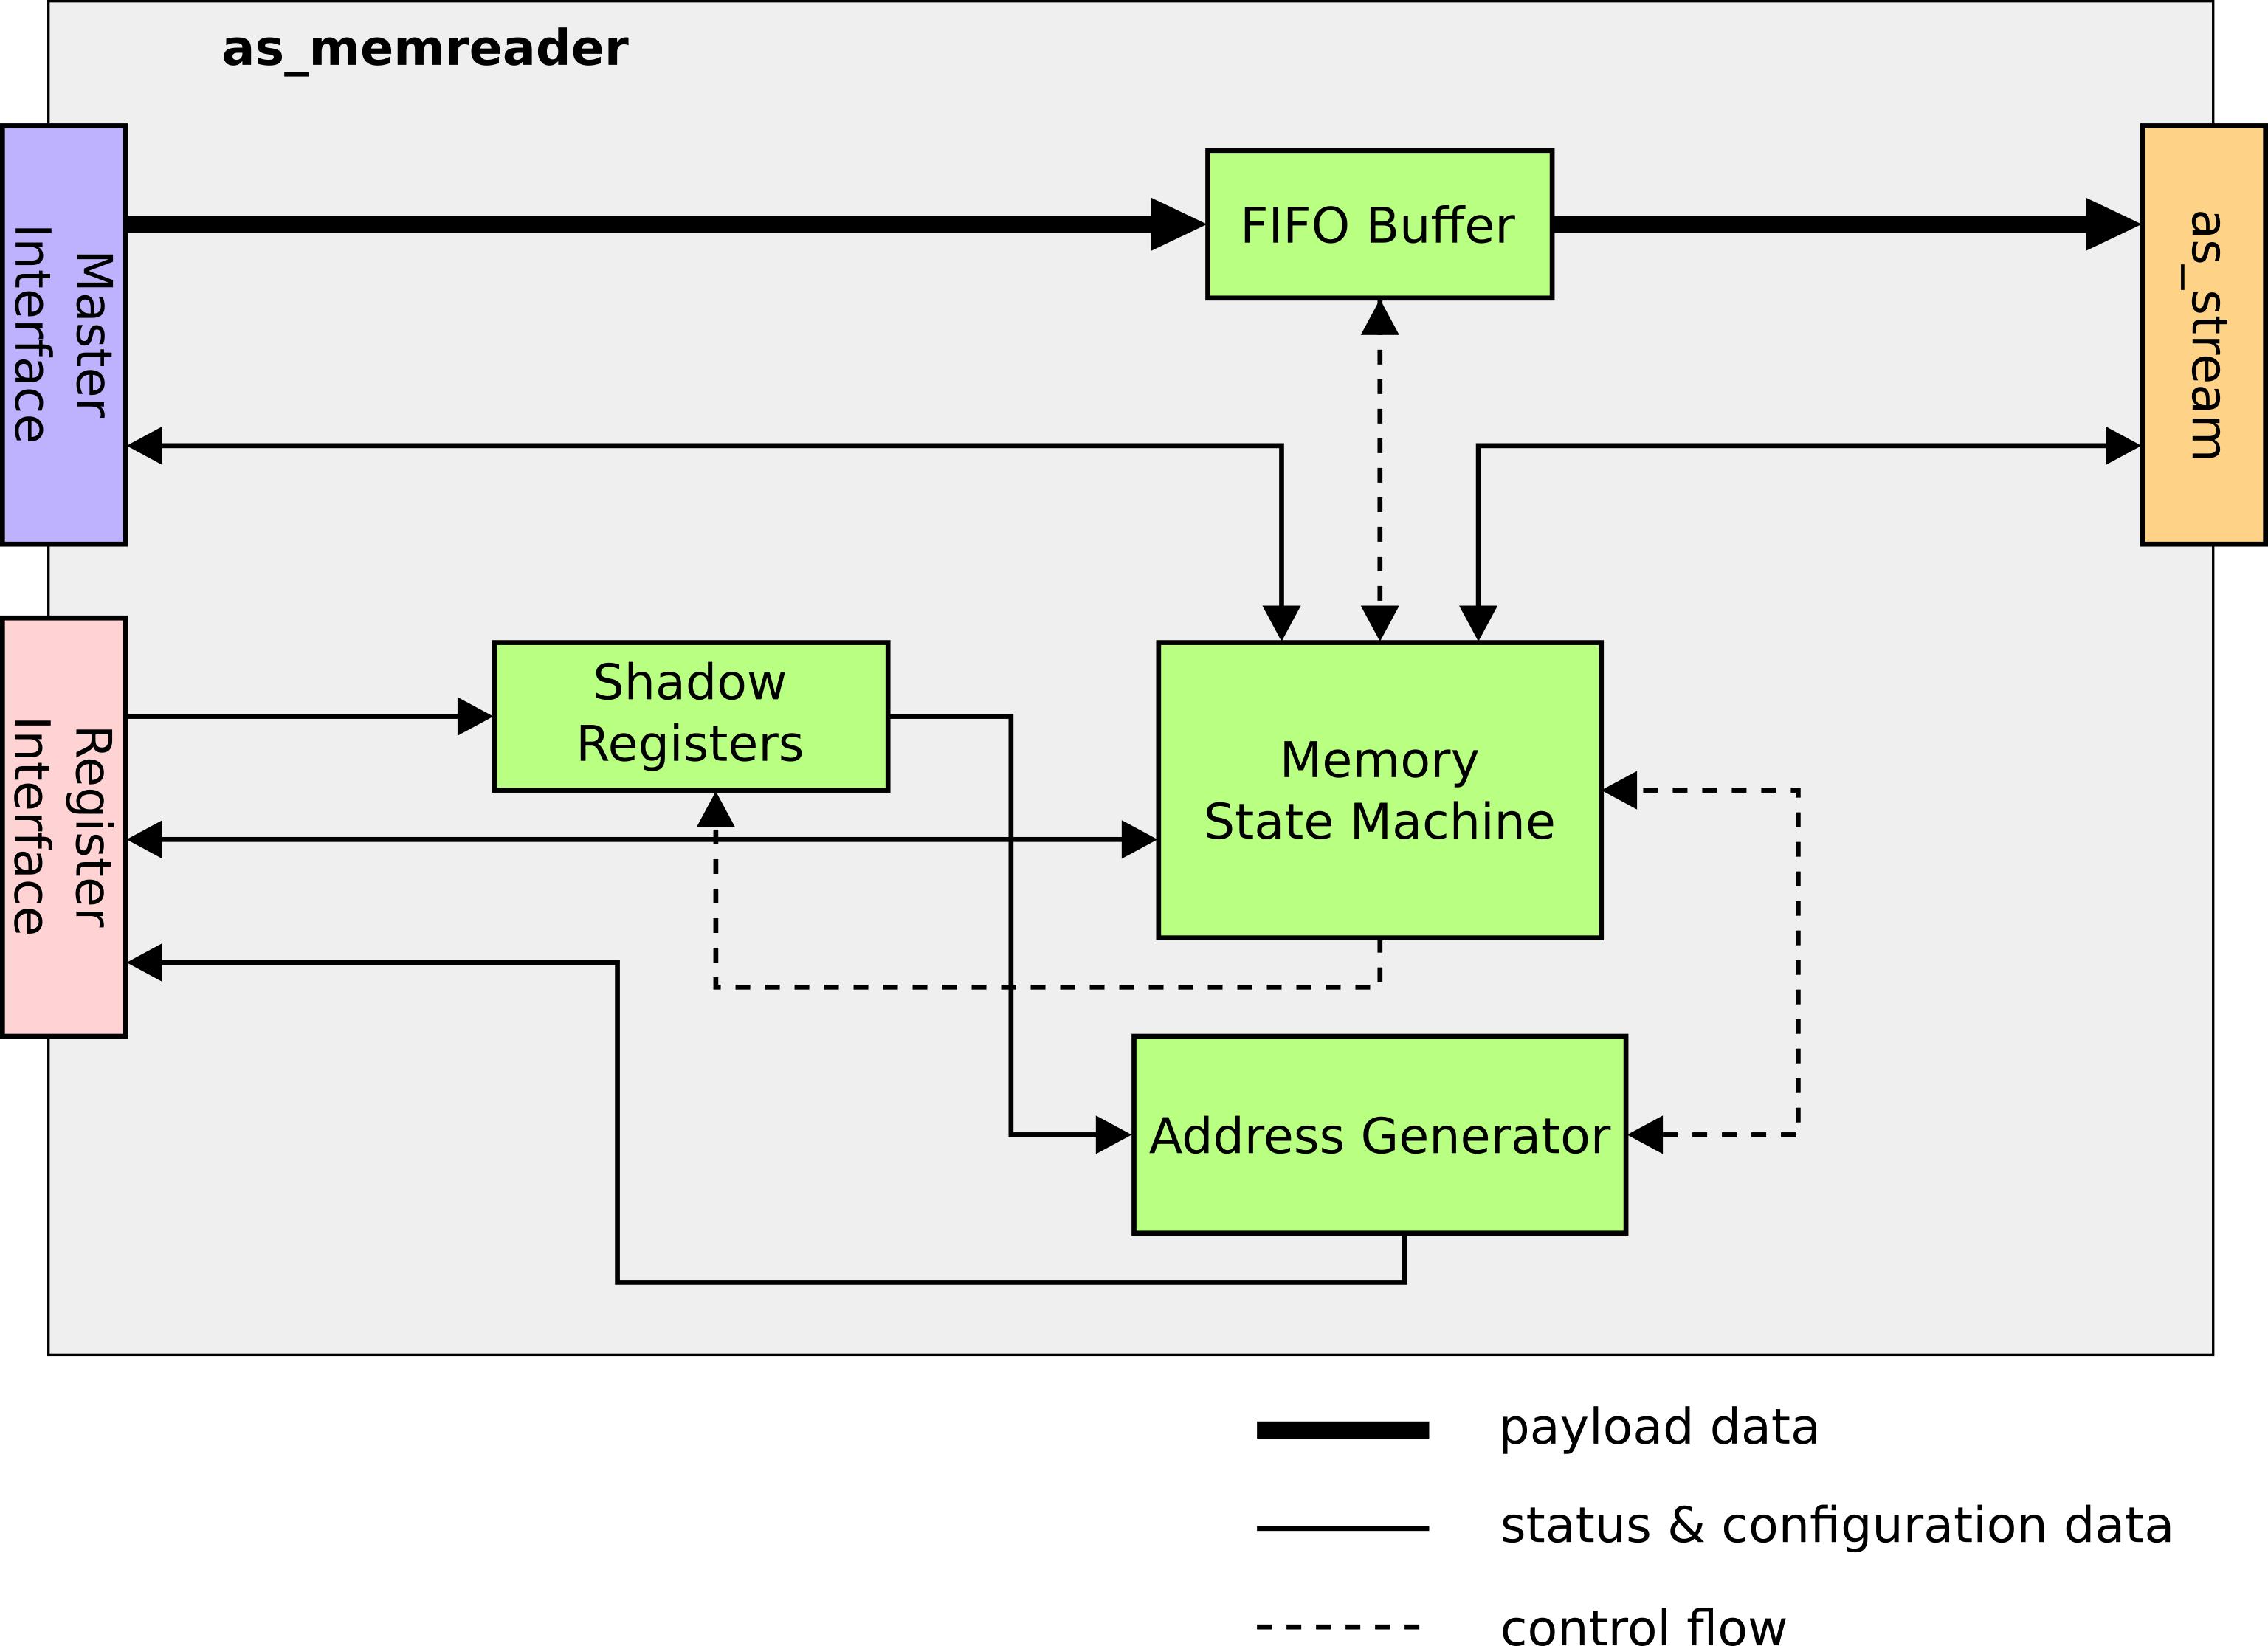
\includegraphics[width=0.8\linewidth,clip]{figs/memreader.png}
    \caption{Architecture of the \texttt{as\_memreader} module}
    \label{fig:memreader}
\end{figure}

\subsubsection{Pre-Synthesis Options}

% TBD(AZ/alle): Diesen Teil und die Layouts sollten wir in einem Meeting
%    diskutieren. @AZ: Sinnvoll ist, meine Kommentare unten vorher noch 
%    einzubauen.

\begin{longtable}[ht]{|l|l|l|}
    \hline
    \multicolumn{1}{|c|}{\textbf{Name}} & \multicolumn{1}{c|}{\textbf{Range}} & \multicolumn{1}{c|}{\textbf{Description}}\\
    \hline
    
    \small{REGISTER\_BIT\_WIDTH} & Positive integer value & \parbox{5cm}{\ \\
        Bit width for the slave registers used by this module (usually 32 bit).\vspace{0.3em}
    }\\
    \hline
    
    \small{DOUT\_WIDTH} & Positive integer value & \parbox{5cm}{\ \\
        Bit width of the data port of this module.\\
        Currently uses the same bit width as the memory bus interface (usually 32 or 64 bit).\vspace{0.3em}
    }\\
    \hline
    
    \small{MEMORY\_DATA\_WIDTH} & Positive integer value & \parbox{5cm}{\ \\
        Bit width of the data port to memory.\\
        Depends on the setting of the memory bus (usually 32 or 64 bit).\vspace{0.3em}
    }\\
    \hline
    
    \small{MEM\_ADDRESS\_BIT\_WIDTH} & Positive integer value & \parbox{5cm}{\ \\
        Bit width of the address port of the memory bus.
        Depends on the memory bus interface (usually 32 bit).\vspace{0.3em}
    }\\
    \hline
    
    \small{BURST\_LENGTH\_BIT\_WIDTH} & Positive integer value & \parbox{5cm}{\ \\
        Bit width of the memory bus to configure the burst size (currently 12 bits).\vspace{0.3em}
    }\\
    \hline
    
    \small{MAX\_PLATFORM\_BURST\_LENGTH} & Positive integer value & \parbox{5cm}{\ \\
        Highest possible burst length support by the memory bus in bytes (currently: 256).\vspace{0.3em}
    }\\
    \hline
    
    \small{FIFO\_NUMBER\_OF\_BURSTS} & Positive integer value & \parbox{5cm}{\ \\
        Minimum size of the internal data fifo. Actual size is to the power of 2 required for fitting the chosen size.\vspace{0.3em}
    }\\
    \hline
    
    \small{SUPPORT\_MULTIPLE\_SECTIONS} & Boolean & \parbox{5cm}{\ \\
        Enables regular address jumps for reading data from memory.\vspace{0.3em}
    }\\
    \hline
    
    \small{SUPPORT\_VARIABLE\_BURST\_LENGTH} & Boolean & \parbox{5cm}{\ \\
        Allows to configure actual burst length at runtime.\vspace{0.3em}
    }\\
    \hline
    
    \small{SUPPORT\_INTERRUPTS} & Boolean & \parbox{5cm}{\ \\
        Allows the module to generate interrupt events.\vspace{0.3em}
    }\\
    \hline
    
    \small{SUPPORT\_DONE\_IRQ\_SOURCE} & Boolean & \parbox{5cm}{\ \\
        Module generates an interrupt event at the end of a \textit{section}.\\
        \small{SUPPORT\_INTERRUPTS} has to be enabled.\vspace{0.3em}
    }\\
    \hline
    
\end{longtable}

\subsubsection{Register Space}

\begin{longtable}[ht]{|l|l|l|l|}
    \hline
    \multicolumn{1}{|c|}{\textbf{Name}} & \multicolumn{1}{c|}{\textbf{Relative Address}} & \multicolumn{1}{c|}{\textbf{Width}} & \multicolumn{1}{c|}{\textbf{Description}}\\
    \hline
    
    \texttt{state/control} & 0x0 & 32 & \parbox{7cm}{\ \\
        Status information of the \texttt{as\_memreader} and controlling the operation of the module. The lower half of the register is used for status information, the upper half for configuration.\vspace{0.3em}
    }\\
    \hline
    
    \texttt{section addr} & 0x4 & 32 & \parbox{7cm}{\ \\
        Memory address at which the module starts to read data from.\vspace{0.3em}
    }\\
    \hline
    
    \texttt{section offset} & 0x8 & 32 & \parbox{7cm}{\ \\
        Address offset in byte for regular address jumps. The offset is the distance between the start addresses of two consecutive \textit{sections}.\vspace{0.3em}
    }\\
    \hline
    
    \texttt{section size} & 0xC & 32 & \parbox{7cm}{\ \\
        Size of a \textit{section} in byte to be read from memory. The size has to be a multiple of the configured data bus width in byte.\vspace{0.3em}
    }\\
    \hline
    
    \texttt{section count} & 0x10 & 32 & \parbox{7cm}{\ \\
        Number of \textit{sections}. If \texttt{SUPPORT\_MULTIPLE\_SECTIONS} is not set, this register is ignored and a single \textit{section} is assumed.\\
        Otherwise, an address jump is performed between two consecutive \textit{sections}.\vspace{0.3em}
    }\\
    \hline
    
    \texttt{max burst length} & 0x14 & 32 & \parbox{7cm}{\ \\
        Number of bytes to be requested for a single memory bus access.\\
        Has to be a multiple of \texttt{MEMORY\_DATA\_WIDTH} and must not exceed \texttt{MAX\_PLATFORM\_BURST\_LENGTH}.\vspace{0.3em}
    }\\
    \hline
    
    \texttt{current hw addr} & 0x18 & 32 & \parbox{7cm}{\ \\
        Next memory address the module is going to read from.\\
        If the \texttt{as\_memreader} is not programmed this address is 0x0.\\
        For multiple \textit{sections}, it points to the last \textit{section} start address + offset after the last \textit{section} has been served.\vspace{0.3em}
    }\\
    \hline
    \caption{Register overview of the \texttt{as\_memreader} module.}
\end{longtable}


\begin{longtable}[ht]{|l|l|l|l|l|}
    \hline
    \multicolumn{1}{|c|}{\textbf{Field Name}} & \multicolumn{1}{c|}{\textbf{Bit Index}} & \multicolumn{1}{c|}{\textbf{Type}} & \multicolumn{1}{c|}{\textbf{Reset Value}} & \multicolumn{1}{c|}{\textbf{Description}}\\
    \hline
    
    \texttt{go} & 17 & wo & 0x0 & \parbox{5cm}{\ \\
        If set, the \texttt{as\_memreader} starts transferring data to memory.\vspace{0.3em}
    }\\
    \hline
    
    \texttt{reset} & 16 & wo & 0x0 & \parbox{5cm}{\ \\
        Resets the module and clears all remaining data in the \textit{FIFO Buffer}.\vspace{0.3em}
    }\\
    \hline
    
    \texttt{pending go} & 5 & ro & 0x0 & \parbox{5cm}{\ \\
        If set, the next data transfer has already been programmed.\vspace{0.3em}
    }\\
    \hline
    
    \texttt{busy} & 1 & ro & 0x0 & \parbox{5cm}{\ \\
        The \texttt{as\_memreader} is currently operating.\vspace{0.3em}
    }\\
    \hline
    
    \texttt{ready} & 0 & ro & 0x0 & \parbox{5cm}{\ \\
        The \texttt{as\_memreader} is currently idle.\vspace{0.3em}
    }\\
    \hline
    \caption{Bit field overview of the combined \texttt{state/control} register of the \texttt{as\_memreader}.}
    \label{table:memreader-state-fields}
\end{longtable}


\begin{longtable}[ht]{|l|l|l|l|l|}
    \hline
    \multicolumn{1}{|c|}{\textbf{Field Name}} & \multicolumn{1}{c|}{\textbf{Bit Index}} & \multicolumn{1}{c|}{\textbf{Type}} & \multicolumn{1}{c|}{\textbf{Reset Value}} & \multicolumn{1}{c|}{\textbf{Description}}\\
    \hline
    
    \texttt{section address} & 31:0 & wo & 0x0 & \parbox{5cm}{\ \\
        Start address for reading data from memory.\vspace{0.3em}
    }\\
    \hline
    
    \caption{Bit field overview of the \texttt{section addr} register of the \texttt{as\_memreader}.}
    \label{table:memreader-section_addr-fields}
\end{longtable}


\begin{longtable}[ht]{|l|l|l|l|l|}
    \hline
    \multicolumn{1}{|c|}{\textbf{Field Name}} & \multicolumn{1}{c|}{\textbf{Bit Index}} & \multicolumn{1}{c|}{\textbf{Type}} & \multicolumn{1}{c|}{\textbf{Reset Value}} & \multicolumn{1}{c|}{\textbf{Description}}\\
    \hline
    
    \texttt{section offet} & 31:0 & wo & 0x0 & \parbox{5cm}{\ \\
        The offset is the distance between two start addresses in byte.\vspace{0.3em}
    }\\
    \hline
    
    \caption{Bit field overview of the \texttt{section offset} register of the \texttt{as\_memreader}.}
    \label{table:memreader-section_offset-fields}
\end{longtable}


\begin{longtable}[ht]{|l|l|l|l|l|}
    \hline
    \multicolumn{1}{|c|}{\textbf{Field Name}} & \multicolumn{1}{c|}{\textbf{Bit Index}} & \multicolumn{1}{c|}{\textbf{Type}} & \multicolumn{1}{c|}{\textbf{Reset Value}} & \multicolumn{1}{c|}{\textbf{Description}}\\
    \hline
    
    \texttt{section size} & 31:0 & wo & 0x0 & \parbox{5cm}{\ \\
        Size of a \textit{section} in byte to be read from memory.\vspace{0.3em}
    }\\
    \hline
    
    \caption{Bit field overview of the \texttt{section size} register of the \texttt{as\_memreader}.}
    \label{table:memreader-section_size-fields}
\end{longtable}


\begin{longtable}[ht]{|l|l|l|l|l|}
    \hline
    \multicolumn{1}{|c|}{\textbf{Field Name}} & \multicolumn{1}{c|}{\textbf{Bit Index}} & \multicolumn{1}{c|}{\textbf{Type}} & \multicolumn{1}{c|}{\textbf{Reset Value}} & \multicolumn{1}{c|}{\textbf{Description}}\\
    \hline
    
    \texttt{section count} & 31:0 & wo & 0x0 & \parbox{5cm}{\ \\
        Number of \textit{sections}.\vspace{0.3em}
    }\\
    \hline
    
    \caption{Bit field overview of the \texttt{section count} register of the \texttt{as\_memreader}.}
    \label{table:memreader-section_count-fields}
\end{longtable}


\begin{longtable}[ht]{|l|l|l|l|l|}
    \hline
    \multicolumn{1}{|c|}{\textbf{Field Name}} & \multicolumn{1}{c|}{\textbf{Bit Index}} & \multicolumn{1}{c|}{\textbf{Type}} & \multicolumn{1}{c|}{\textbf{Reset Value}} & \multicolumn{1}{c|}{\textbf{Description}}\\
    \hline
    
    \texttt{max burst length} & 31:0 & wo & 0x0 & \parbox{5cm}{\ \\
        Number of bytes to be requested for a single memory bus access.\vspace{0.3em}
    }\\
    \hline
    
    \caption{Bit field overview of the \texttt{max burst length} register of the \texttt{as\_memreader}.}
    \label{table:memreader-burst-fields}
\end{longtable}


\begin{longtable}[ht]{|l|l|l|l|l|}
    \hline
    \multicolumn{1}{|c|}{\textbf{Field Name}} & \multicolumn{1}{c|}{\textbf{Bit Index}} & \multicolumn{1}{c|}{\textbf{Type}} & \multicolumn{1}{c|}{\textbf{Reset Value}} & \multicolumn{1}{c|}{\textbf{Description}}\\
    \hline
    
    \texttt{current hw addr} & 31:0 & ro & 0x0 & \parbox{5cm}{\ \\
        Next address the \texttt{as\_memreader} is going to read from.\vspace{0.3em}
    }\\
    \hline
    
    \caption{Bit field overview of the \texttt{current hw addr} register of the \texttt{as\_memreader}.}
    \label{table:memreader-cur_hw-fields}
\end{longtable}

\subsubsection{Behavior}
The bit fields of the \texttt{control} and \texttt{state} registers are also represented internally within the module by signals with the same name.
When referring to the bit field, the name is written in lower case and in upper case for the signal.
Flags refer to the bit fields.

% Start up and reset (during reset, post reset)
When the module receives a reset request, either by using the hardware port or the \texttt{reset} flag of the \textit{State Control} register, ongoing bus accesses are terminated and all internally stored configuration settings are cleared after a single clock cycle.
Additionally, the module requests to clear the \texttt{go} and \texttt{reset} field.
The configuration registers towards software are left as is.
Simultaneously, the data in the \textit{FIFO Buffer} is discarded and the address generator is reset.
The reset persists only for one clock cycle if it has been requested by software, otherwise up to the point it is lifted by hardware.
During the reset, neither of the modules' status flags is set.
After the reset has been lifted, the \texttt{as\_memreader} assumes its idle state.


% Operation
In the modules' idle state, the \texttt{ready} flag is set and the configuration registers are continuously copied into internal shadow registers.
Upon setting the \texttt{go} field, the current configuration is used for setting up data transfers after one clock cycle.
Further, the \texttt{ready} flag is unset and the \texttt{busy} flag is set instead, which is kept throughout the whole operation.
The \texttt{as\_memreader} requests the slave logic to clear the \texttt{go} flag and starts accessing the master memory bus interface.
During operation, the configuration registers can be overwritten and \texttt{go} flag set again, to seamlessly queue the next data transfer.
If the \texttt{go} flag was set in this manner, the module sets its \texttt{PENDING GO} signal.
Since the \texttt{as\_memreader} copies the configuration only at the start, it would be possible to change the configuration for the following transfer after having already set the \texttt{go} flag again.
However, it is strongly recommended to configure the data transfer before queuing the next transmission.
As soon as the \texttt{as\_memreader} has read all requested data for the current operation, it sets the \texttt{ready} flag again and returns to its idle state.
Here, the \texttt{busy} and \texttt{ready} flag are set simultaneously for a single clock cycle, which is exclusively used if another hardware module interfaces the \texttt{as\_memwriter} instead of software.
This is mainly for backwards compatibility and may be subject to change in the future.
If the next \texttt{GO} has already been set when entering the idle state, the module proceeds in the aforementioned manner without delay.
The \texttt{PENDING GO} (since \texttt{GO} is unset) is unset again.


% Stall
The \texttt{as\_memreader} is a \textit{stall-absorbing} module (see Chapter~\ref{05-03-stall}), which means it accepts requests to suspend data transfers by the following module.
After receiving a stall request, the \texttt{as\_memreader} stops transferring data at its \textit{as\_stream} output interface on the following clock cycle, until the stall is lifted again.
Since the module utilizes a \textit{FIFO Buffer}, it continues to read data from memory if there is remaining space.
The fifo is considered full, if it can only hold the equivalent of one additional maximal possible burst length amount of data.
Since the actually utilized burst length may vary (if \texttt{SUPPORT\_VARIABLE\_BURST\_LENGTH} is set), this method allows to prevent \textit{FIFO Buffer} overflow without having to check the precise amount of space left for each memory bus request.
This method has mainly been chosen to prevent the module from inefficiently reading multiple small amounts of data in order to utilize the whole \textit{FIFO Buffer}.
Instead, if the aforementioned threshold has been reached, the \texttt{as\_memreader} suspends reading data from memory until the \textit{FIFO Buffer} has output some data.
As a side effect, some FPGA area has been saved which would be required for the comparison.


% Support multiple sections
The \texttt{as\_memreader} module organizes its data transfers in one or more \textit{sections}, where each one is a physically continuous chunk of data in memory.
If more than one \textit{section} is required, the configuration option \texttt{SUPPORT\_MULTIPLE\_SECTIONS} has to be set at synthesis time.
The register \textit{Section Address} defines the memory address of the first \textit{section}, whereas \textit{Section Offset} is used for the following ones.
The latter is the difference of the start addresses of two consecutive \textit{sections}.
For example, if the first \textit{section} starts at the hexadecimal address "0x2000" and the following one at "0x5000", an offset of "0x3000" has to be configured.
The third \textit{section} would start at address "0x8000".
The number of \textit{sections} are chosen by writing a number greater 1 to the register \textit{Section Count}.
The size of a single \textit{section} is configured by using \textit{Section Size}.
When using more than one \textit{section}, the configured size should not exceed the offset, since it would result in partially overwriting the preceding \textit{section} with the following one.
If the value of \textit{Section Size} is less than \textit{Section Offset}, the difference between two \textit{sections} is skipped.
Assuming the above example with a size of "0x2200", the address range from "0x4200" to "0x4fff" is skipped and therefore not read from memory.
This method can be used for reading a sub-image from memory or skipping regular areas of a certain data layout.
If \texttt{SUPPORT\ MULTIPLE\ SECTIONS} is not set, \textit{Section Offset} and \textit{Section Count} are ignored and a single \textit{section} is assumed.


% Current hw addr
After starting the operation of the \texttt{as\_memreader} for the first time by setting the \texttt{GO} signal, the module continuously provides the current physical memory address of the \textit{Address Generator} to the software.
This address is the one used for the next memory access but might not have been processed yet.
It is stored within the hardware register \texttt{current hw addr}.
At the end of the operation of the \texttt{as\_memreader}, the address within this register points at the first address following the current \textit{section} if \texttt{SUPPORT\_MULTIPLE\_SECTIONS} has been set to "false".
Otherwise, it points at the start address of the following \textit{section}, although it is not used.
This is due to the fact, that the address is incremented by the \textit{offset} after each \textit{section}, where the last one is not handled separately.
The address is only updated during the operation of the \texttt{as\_memreader} and therefore is also not cleared once it has finished its operation.
However, performing a \textit{reset} on the module, either by hardware or software, clears the register.


% Variable burst length
The \texttt{as\_memreader} preferably utilizes burst accesses to read a chunk of memory at once, since requesting the memory bus requires a considerable overhead.
By using bursts, the number of bus accesses and therefor required overhead can be reduced.
The number of bytes used for a burst access can be configured using the register \textit{Maximal Burst Length}.
The configured number of bytes written to this register has to be a multiple of the of the memory bus interface.
Additionally, the maximal amount of data transferred in a single burst is usually limited by the architecture, to prevent other bus masters from starving, which must not be exceeded.
If the configured \textit{Section Size} is not a multiple of \textit{Maximal Burst Length}, the \texttt{as\_memreader} module falls back to less efficient single beat accesses for the remaining bytes, if \texttt{SUPPORT\_VARIABLE\_BURST\_LENGTH} has not been set.
The module requests the number of bytes equal to the one used for the memory bus interface at a time, which is usually 4 or 8 bytes.
If \texttt{SUPPORT\_VARIABLE\_BURST\_LENGTH} has been set, however, the \texttt{as\_memreader} performs a burst access for equal to the remaining number of bytes.\newline


% Error handling
The \texttt{as\_memreader} module does not perform any kind of error handling (see Chapter~\ref{ch:05-02-interfaces-module_signals}).
Since the module is designed to actively "pull" data, a \texttt{SYNC\_ERROR} due to lost data cannot occur.
Additionally, the \texttt{as\_memreader} is not able to determine whether its received data posses a valid value and therefore does not generate a \texttt{DATA\_ERROR} either.


% as\_arbiter
Instead of directly utilizing a memory bus master, the \texttt{as\_memreader} module can also be connected to an \textit{as\_arbiter} for mapping multiple \asterics memory modules to a single memory bus master.
The \texttt{as\_memreader} requests a bus access by setting the port \texttt{mem\_req} to "1" and subsequently for the same value appearing at its \texttt{mem\_req\_ack} port.
The latter port has to be bound to "1" (high), if no \textit{as\_arbiter} is used.


% Interrupt
Optionally, the \texttt{as\_memreader} generates a high level ("1") at its \texttt{interrupt\_out} port when it finishes its configured data transfer operation, i.e. all \textit{sections} have been read from memory.
Therefor, the pre-synthesis parameters \texttt{SUPPORT\_INTERRUPTS} and \texttt{SUPPORT\_DONE\_IRQ\_SOURCE} have to be set to "true".
The signal is active for a single clock cycle and can be used for generating a hardware interrupt for the processor, by using one of the available interrupt lines.


\subsubsection{Module Driver}
In order to set up data transfers from software, a module driver, namely \texttt{as\_reader\_writer}, is provided for the \texttt{as\_memreader}.
This driver is implemented in \textit{C} and comprises a header and a source file.
Within the module driver, a number of macros are defined for calculating the offset of the hardware registers and their bit indices.
These macros can be used for interfacing the hardware registers of the \texttt{as\_memreader} manually.
Alternatively, the functions of the module driver can be used. 
The provided functions enable to utilize the functionality of the module without having to look up the appropriate macros.
Internally, the \textit{\asterics Support Library} is used for performing the actual accesses to hardware.

\subsubsection{Application Notes}
For common applications using \texttt{as\_memreader} module, the default settings for most of its pre-synthesis parameters can be used.
The only exception is \texttt{DOUT\_WIDTH} and \texttt{MEMORY\_DATA\_WIDTH} which may be adjusted to 64 bit.
The following Listing~\ref{lst:memreader_setup} shows how the \texttt{as\_memreader} module is usually set up for a bare-metal application.
For using the module with an operating system, the device driver of the \asterics framework has to be used (see Chapter~\ref{ch:04-05-software-linux}).
As a first step, the registers of the module are set by using the function \texttt{as\_reader\_writer\_init()}.
It takes two arguments, the start address of the module, which is defined in \textit{as\_hardware.h}, and a pointer to the configuration structure \texttt{as\_reader\_writer\_config\_t} defined in the header file of the module driver.
By allocating a structure of this type, the corresponding data fields can be set in advance, to configure the module at once.
If a NULL pointer is provided to \texttt{as\_reader\_writer\_init()}, the default values defined in the header file are used, which covers most applications.
The function also resets the hardware module.
The \textit{section address} and \textit{section size} have to be manually configured by the user by using \texttt{as\_reader\_writer\_set\_section\_addr()} and \texttt{as\_reader\_writer\_set\_section\_size()} respectively.
A default \textit{section size} is set by \texttt{as\_reader\_writer\_init()}, however, the value is likely to differ from what is required by the user.
Lastly, \texttt{as\_reader\_writer\_set\_go()} starts the operation.
For some applications it may be required to check whether the module has completed its operation by using \texttt{as\_reader\_writer\_is\_done()}.
The given example shows an active status polling of the device, but different methods may also be used.


\begin{footnotesize}
    \lstset{style=CStyle, caption={Using the \texttt{as\_memreader} module.}}
    \begin{lstlisting}[label=lst:memreader_setup]
    /* Define a section size; here: the resolution of an image in 
       byte */ 
    #define IMAGE_RES           640*480
    
    /* Allocate a memory area */
    void *image_address = as_malloc(IMAGE_RES);
    
    
    /******* Setting up the as_memreader module *******/
    
    /* Sets default values for burst length, etc. */
    as_reader_writer_init(AS_MODULE_BASEADDR_MEMREADER_0, NULL);
    
    /* Set the start address, where the as_memreader is supposed to 
       read from */
    as_reader_writer_set_section_addr( \
        AS_MODULE_BASEADDR_MEMREADER_0, \
        (uint32_t*) image_address);
    
    /* Set the number of bytes to be read */
    as_reader_writer_set_section_size( \
        AS_MODULE_BASEADDR_MEMREADER_0, IMAGE_RES)
    
    
    /************** Data transfer **************/
    
    /* Start the as_memreader */
    as_reader_writer_set_go(AS_MODULE_BASEADDR_MEMREADER_0);
    
    /* Wait until the as_memreader has completed the section */
    while(!as_reader_writer_is_done( \
        AS_MODULE_BASEADDR_MEMREADER_0)) {
    /* Do nothing */
    }
    \end{lstlisting}
\end{footnotesize}


\subsection{as\_memwriter} \label{ch:07-basic-mods-in_out-memwriter}

\secauthor{Alexander Zoellner}

\subsubsection{Brief Description}

The \texttt{as\_memwriter} is a hardware module for efficiently transferring data from the FPGA to main memory.
The module utilizes an \textit{as\_stream} interface to programmable logic and a bus master interface to memory.
It transfers chunks of data , so called \textit{sections}, by using burst accesses whenever possible.
\textit{Sections} are defined by a start address and size.
Multiple \textit{sections} are also supported, which may include a constant offset (i.e. the difference between the start address of two consecutive \textit{sections}) in between, allowing to write rectangular sub-images or complying to a certain data layout.
In order to decrease the amount of time spent idle, the following \textit{section} can be programmed during an ongoing operation by overwriting the hardware registers of the \texttt{as\_memwriter} and setting its \texttt{go} flag again.
The module proceeds with the next data transfer after the current \textit{section} has been completed, i.e. all data has been written.
The module provides a register for tracking the progress of the current \textit{section}, which holds the next address the module is going to read from.
Additionally, the \texttt{as\_memwriter} supports organizing data in \textit{data units}, which is a logically grouped number of bytes.
A counter, readable by software, is used for tracking the number of \textit{data units}, which have been transferred to memory.
This can be used for counting frames, image lines or any arbitrary data sets.

\subsubsection{Architecture}

Figure~\ref{fig:memwriter} shows the architecture of the \texttt{as\_memwriter} module in simplified form to emphasize the main parts of the module, which are required for performing data transfers. 
The \texttt{as\_memwriter} obtains its data via a hardware module, using the \texttt{as\_stream} interface (see Chapter~\ref{ch:05-03-interfaces-as_stream}).
The incoming data is intermediately stored in a \textit{FIFO Buffer}, in order to aggregate a certain number of bytes for performing more efficient data transfers towards memory, using \textit{bursts}.
Further, data loss is prevented in this manner, if access to the memory bus cannot be obtained right away.
If the \textit{FIFO Buffer} reaches its limit, the \texttt{as\_memwriter} requests the preceding module to suspend any further data transfers to its \texttt{as\_stream} interface.
The \texttt{as\_memwriter} utilizes a \textit{Master Interface} for transferring data to memory.
This interface comprises only signals which are required for configuring the access to memory, such as the number of bytes to be transferred or when to start a data transfer. 
The actual memory bus access is performed by a \textit{Bus Translation} module, which is connected to the memory bus interface and the \texttt{as\_memwriter}.
Occasionally, the user may not require the data of the image processing chain, which results in the \texttt{as\_memwriter} to not transfer any data to memory.
In this case, the \textit{Enable Logic} is used to discard any following data at the \texttt{as\_stream} interface, to prevent the \textit{FIFO Buffer} from overflowing.
Thus, the \texttt{as\_memwriter} does not have to request the preceding module to suspend its data transfers, since other parts of the processing chain may depend on the data (e.g. the \texttt{as\_memwriter} is only used to store intermediate results for control purposes).
For regular operation, the \textit{Enable Logic} merely forwards the data to the \textit{FIFO Buffer}.

For configuring the \texttt{as\_memwriter}, a \textit{Register Interface} is utilized, which are associated with a number of hardware registers. 
These registers can be accessed by hardware and software alike, for exchanging control and status information. 
The control information are provided by software via the \textit{Register Interface} to affect the behavior of the \texttt{as\_memwriter}.
For this reason, the appropriate hardware registers are connected to the \textit{Enable Logic} to choose whether the \texttt{as\_memwriter} is expected to discard data at its \texttt{as\_stream} interface.
The \textit{Memory State Machine} is the central part of the module and is responsible for setting up data transfers, according to the settings of the software within the hardware registers.
It also affects the \textit{Enable Logic} under certain conditions.

During an ongoing operation, certain information must not be changed, in order for the \texttt{as\_memwriter} module to operate correctly. 
For this reason, information regarding the specifics of the operation, such as number of \textit{sections} or its size, have to be kept stable. 
This is accomplished by copying critical information to \textit{Shadow Registers} at the start of an operation, which is determined by the \textit{Memory State Machine}. 
As a side effect, this allows the software to replace the associated hardware registers during an ongoing operation, which is used for queuing the subsequent operation for transferring data. 
The \textit{Address Generator} calculates the address required for the individual memory accesses as well as the number of bytes to be transferred. 
The required information are obtained from the \textit{Shadow Registers}. 
Towards software, the address used for the next data transfer is published to software via the \textit{Register Interface}.

Optionally, the \textit{Data Unit Complete Logic} can be added to the \texttt{as\_memwriter} if \texttt{SUPPORT\_DATA\_UNIT\_COMPLETE} has been set.
It is used for tracking the number of \textit{data units} which have been transferred to memory.
This number as well as the end address of the last \textit{data unit} is published to software using the \textit{Register Interface}.
For certain configurations, the \textit{Data Unit Complete Logic} also affects the \textit{Enable Logic}.


\begin{figure}[ht]
    \centering
    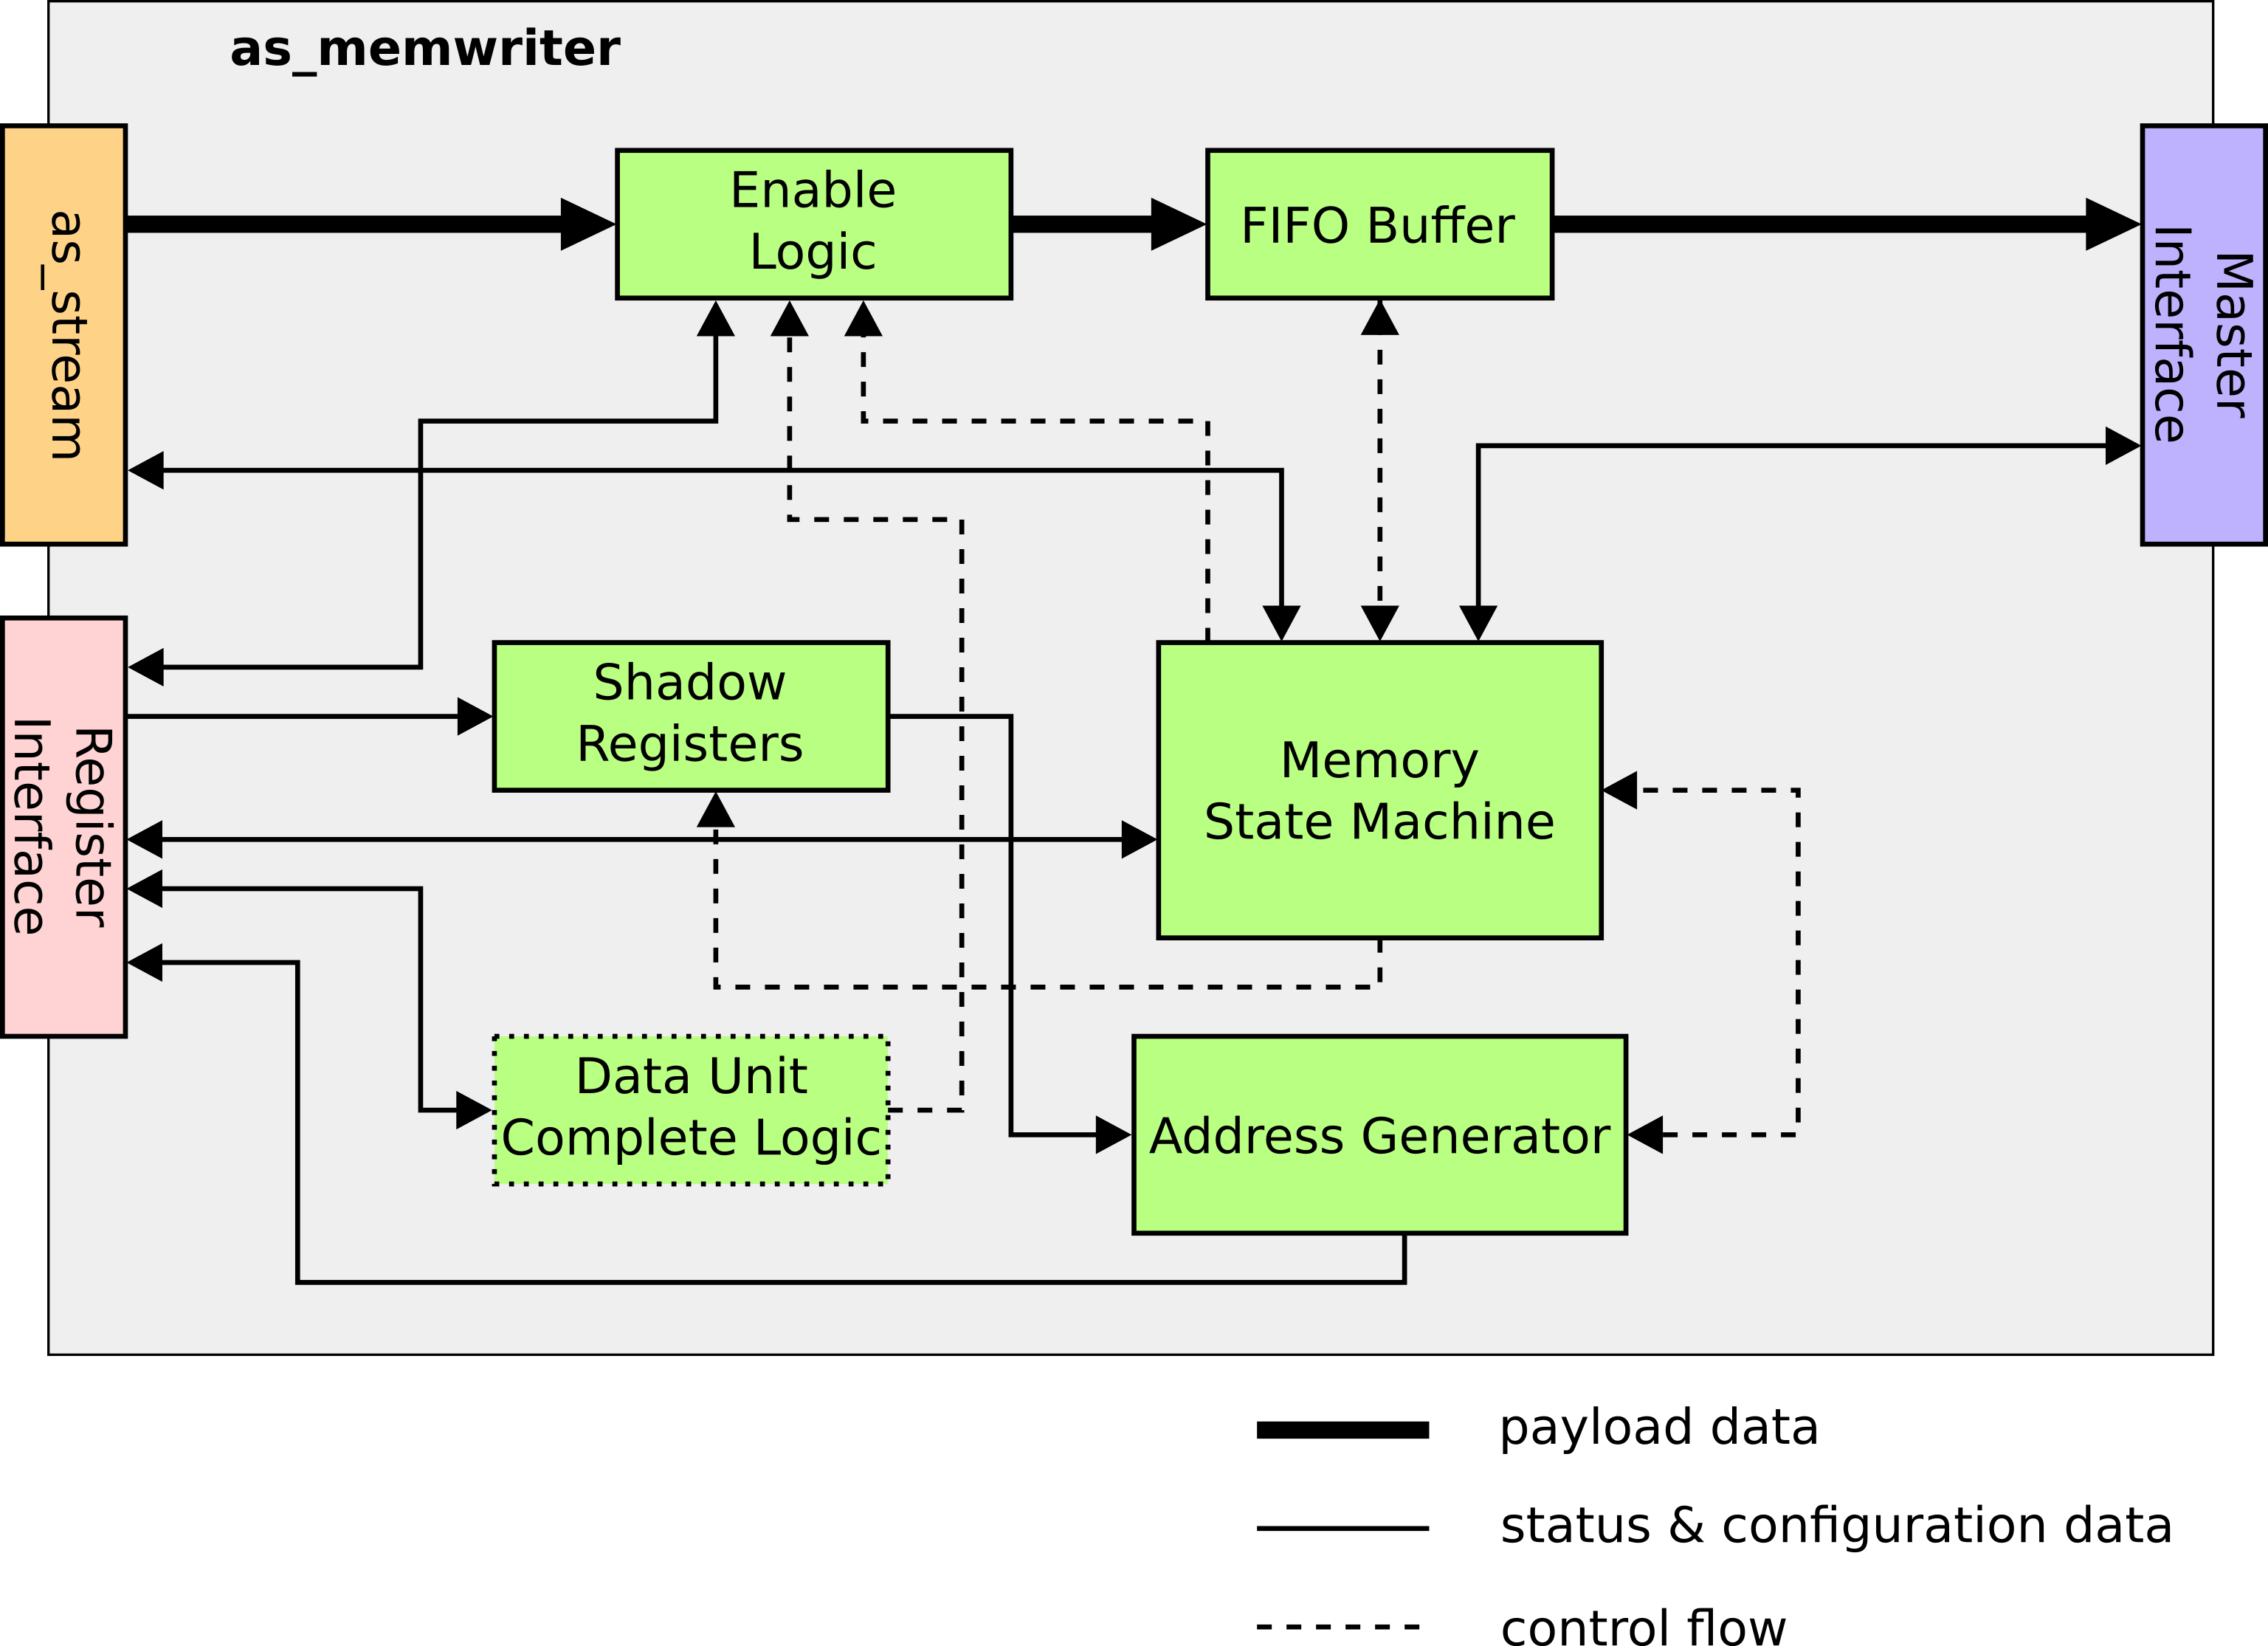
\includegraphics[width=0.8\linewidth,clip]{figs/memwriter.png}
    \caption{Architecture of the \texttt{as\_memwriter} module}
    \label{fig:memwriter}
\end{figure}

\subsubsection{Pre-Synthesis Options}

\begin{longtable}[ht]{|l|l|l|}
    \hline
    \multicolumn{1}{|c|}{\textbf{Name}} & \multicolumn{1}{c|}{\textbf{Range}} & \multicolumn{1}{c|}{\textbf{Description}}\\
    \hline
    
    \small{REGISTER\_BIT\_WIDTH} & Positive integer value & \parbox{5cm}{\ \\
        Bit width for the slave registers used by this module (usually 32 bit).\\
    }\\
    \hline
    
    \small{DOUT\_WIDTH} & Positive integer value & \parbox{5cm}{\ \\
        Bit width of the data port of this module.\\
        Currently uses the same bit width as the memory bus interface (usually 32 or 64 bit).\\
    }\\
    \hline
    
    \small{MEMORY\_DATA\_WIDTH} & Positive integer value & \parbox{5cm}{\ \\
        Bit width of the data port to memory.\\
        Depends on the setting of the memory bus (usually 32 or 64 bit).\\
    }\\
    \hline
    
    \small{MEM\_ADDRESS\_BIT\_WIDTH} & Positive integer value & \parbox{5cm}{\ \\
        Bit width of the address port of the memory bus.\\
        Depends on the memory bus interface (usually 32 bit).
    }\\
    \hline
    
    \small{BURST\_LENGTH\_BIT\_WIDTH} & Positive integer value & \parbox{5cm}{\ \\
        Bit width of the memory bus to configure the burst size (currently 12 bits).\\
    }\\
    \hline
    
    \small{MAX\_PLATFORM\_BURST\_LENGTH} & Positive integer value & \parbox{5cm}{\ \\
        Highest possible burst length support by the memory bus in bytes (currently: 256).\\
    }\\
    \hline
    
    \small{FIFO\_NUMBER\_OF\_BURSTS} & Positive integer value & \parbox{5cm}{\ \\
        Minimum size of the internal data fifo. The actual size is to the power of 2 required for fitting the chosen size.\\
    }\\
    \hline
    
    \small{SUPPORT\_MULTIPLE\_SECTIONS} & Boolean & \parbox{5cm}{\ \\
        Enables regular address jumps for reading data from memory.\\
    }\\
    \hline
    
    
    \small{SUPPORT\_INTERRUPTS} & Boolean & \parbox{5cm}{\ \\
        Allows the module to generate interrupt events.\\
    }\\
    \hline
    
    \small{SUPPORT\_DONE\_IRQ\_SOURCE} & Boolean & \parbox{5cm}{\ \\
        Module generates an interrupt event at the end of a \textit{section}.\\
        \small{SUPPORT\_INTERRUPTS} has to be enabled.\\
    }\\
    \hline
    
    \small{SUPPORT\_DUC\_IRQ\_SOURCE} & Boolean & \parbox{5cm}{\ \\
        Module generates an interrupt event at the end of a data unit.\\
        \small{SUPPORT\_INTERRUPTS} has to be enabled.\\
        \small{SUPPORT\_DATA\_UNIT\_}\\
        \small{COMPLETE} has to be enabled.\\
    }\\
    \hline
    
    \small{SUPPORT\_DATA\_UNIT\_COMPLETE} & Boolean & \parbox{5cm}{\ \\
        Module generates an interrupt event at the end of a data unit.\\
        \small{SUPPORT\_INTERRUPTS} has to be enabled.\\
    }\\
    \hline
    
    \small{UNIT\_COUNTER\_WIDTH} & Positive integer value & \parbox{5cm}{\ \\
        Bit width of the register for storing the number of data units.\\
    }\\
    \hline
    
\end{longtable}

\subsubsection{Register Space}

\begin{longtable}[ht]{|l|l|l|l|}
    \hline
    \multicolumn{1}{|c|}{\textbf{Name}} & \multicolumn{1}{c|}{\textbf{Relative Address}} & \multicolumn{1}{c|}{\textbf{Width}} & \multicolumn{1}{c|}{\textbf{Description}}\\
    \hline
    
    \texttt{state/control} & 0x0 & 32 & \parbox{7cm}{\ \\
        Status information of the \texttt{as\_memwriter} and controlling the operation of the module. The lower half of the register is used for status information, the upper half for configuration.\\
    }\\
    \hline
    
    \texttt{ section addr} & 0x4 & 32 & \parbox{7cm}{\ \\
        Memory address at which the module starts to read data from.\\
    }\\
    \hline
    
    \texttt{section offset} & 0x8 & 32 & \parbox{7cm}{\ \\
        Address offset in byte for regular address jumps. The offset is the distance between the start addresses of two consecutive \textit{sections}.\\
    }\\
    \hline
    
    \texttt{section size} & 0xC & 32 & \parbox{7cm}{\ \\
        Size of a \textit{section} in byte to be read from memory. The size has to be a multiple of the configured data bus width in byte.\\
    }\\
    \hline
    
    \texttt{section count} & 0x10 & 32 & \parbox{7cm}{\ \\
        Number of \textit{sections}. If \texttt{SUPPORT\_MULTIPLE\_SECTIONS} is not set, this register is ignored and a single \textit{section} is assumed.\\
        Otherwise, an address jump is performed between two consecutive \textit{sections}.\\
    }\\
    \hline
    
    \texttt{max burst length} & 0x14 & 32 & \parbox{7cm}{\ \\
        Number of bytes to be requested for a single memory bus access.\\
        It has to be a multiple of \texttt{MEMORY\_DATA\_WIDTH} and must not exceed \texttt{MAX\_PLATFORM\_BURST\_LENGTH}.\\
    }\\
    \hline
    
    \texttt{current hw addr} & 0x18 & 32 & \parbox{7cm}{\ \\
        Contains the next memory address the module is going to read from.\\
        If the \texttt{as\_memwriter} is not programmed this address is 0x0.\\
        For multiple \textit{sections}, it points to the last \textit{section} start address + offset after the last \textit{section} has been served.\\
    }\\
    \hline
    
    \parbox{3cm}{\texttt{last data unit complete addr}} & 0x1C & 32 & \parbox{7cm}{\ \\
        Following address after a data unit has been written to memory.\\
        \texttt{SUPPORT\_DATA\_UNIT\_}\small{COMPLETE} has to be set. Otherwise the value of this register is always 0x0.\\
    }\\
    \hline
    
    \texttt{current unit count} & 0x20 & 32 & \parbox{7cm}{\ \\
        Number of transferred data units to memory.\\
        \texttt{SUPPORT\_DATA\_UNIT\_}\small{COMPLETE} has to be set. Otherwise the value of this register is always 0x0.\\
        The actual number of utilized bits of this register depend on the setting of \texttt{UNIT\_COUNTER\_WITDH}, up to 32.
    }\\
    \hline
    
    \caption{Register overview of the \texttt{as\_memwriter} module.}
\end{longtable}

\begin{longtable}[ht]{|l|l|l|l|l|}
    \hline
    \multicolumn{1}{|c|}{\textbf{Field Name}} & \multicolumn{1}{c|}{\textbf{Bit Index}} & \multicolumn{1}{c|}{\textbf{Type}} & \multicolumn{1}{c|}{\textbf{Reset Value}} & \multicolumn{1}{c|}{\textbf{Description}}\\
    \hline
    
    \texttt{flush data} & 23 & wo & 0x0 & \parbox{5cm}{\ \\
        If set, the \texttt{as\_memwriter} to transfer all currently buffered data to memory.\\
    }\\
    \hline
    
    \texttt{disable on no go} & 22 & wo & 0x0 & \parbox{5cm}{\ \\
        If set, the \texttt{as\_memwriter} to reject data at its input port after finishing its current operation and the next one has not been set up (i.e. there is no \texttt{pending go}).\\
    }\\
    \hline
    
    \texttt{single shot} & 21 & wo & 0x0 & \parbox{5cm}{\ \\
        If set, the \texttt{as\_memwriter} only transfers a single \textit{data unit} before it continuous to reject incoming data.\\
    }\\
    \hline
    
    \parbox{3cm}{\texttt{enable on data unit complete}} & 20 & wo & 0x0 & \parbox{5cm}{\ \\
        If set, the \texttt{as\_memwriter} starts accepting data at its input port after receiving a signal at its \texttt{data\_unit\_complete\_in} port.\\
    }\\
    \hline
    
    \texttt{disable} & 19 & wo & 0x0 & \parbox{5cm}{\ \\
        If set, the \texttt{as\_memwriter} rejects all incoming data.\\
    }\\
    \hline
    
    \texttt{enable} & 18 & wo & 0x0 & \parbox{5cm}{\ \\
        If set, the \texttt{as\_memwriter} accepts incoming data.\\
    }\\
    \hline
    
    \texttt{go} & 17 & wo & 0x0 & \parbox{5cm}{\ \\
        If set, the \texttt{as\_memwriter} starts transferring data to memory.\\
    }\\
    \hline
    
    \texttt{reset} & 16 & wo & 0x0 & \parbox{5cm}{\ \\
        Resets the module and clears all remaining data in the \textit{FIFO Buffer}.\\
    }\\
    \hline
    
    \texttt{set enable} & 6 & ro & 0x0 & \parbox{5cm}{\ \\
        If set, the \texttt{as\_memwriter} currently accepts incoming data.\\
    }\\
    \hline
    
    \texttt{pending go} & 5 & ro & 0x0 & \parbox{5cm}{\ \\
        If set, the next data transfer has already been programmed.\\
    }\\
    \hline
    
    \texttt{flushable data} & 4 & ro & 0x0 & \parbox{5cm}{\ \\
        If set, there is currently data in the \textit{FIFO Buffer}, which can be flushed.\\
    }\\
    \hline
    
    \texttt{sync error} & 3 & ro & 0x0 & \parbox{5cm}{\ \\
        If set, data has been lost due to the preceding modules ignoring the \texttt{STALL} signal and the \textit{FIFO Buffer} being full.\\
    }\\
    \hline
    
    \texttt{busy} & 1 & ro & 0x0 & \parbox{5cm}{\ \\
        The \texttt{as\_memwriter} is currently operating.\\
    }\\
    \hline
    
    \texttt{ready} & 0 & ro & 0x0 & \parbox{5cm}{\ \\
        The as\_memwriter is currently idle.\\
    }\\
    \hline
    \caption{Bit field overview of the combined \texttt{state/control} register of the \texttt{as\_memwriter}.}
    \label{table:memwriter-state-fields}
\end{longtable}

\begin{longtable}[ht]{|l|l|l|l|l|}
    \hline
    \multicolumn{1}{|c|}{\textbf{Field Name}} & \multicolumn{1}{c|}{\textbf{Bit Index}} & \multicolumn{1}{c|}{\textbf{Type}} & \multicolumn{1}{c|}{\textbf{Reset Value}} & \multicolumn{1}{c|}{\textbf{Description}}\\
    \hline
    
    \texttt{section address} & 31:0 & wo & 0x0 & \parbox{5cm}{\ \\
        Start address for reading data from memory.\\
    }\\
    \hline
    
    \caption{Bit field overview of the \texttt{section addr} register of the \texttt{as\_memwriter}.}
    \label{table:memwriter-section_addr-fields}
\end{longtable}


\begin{longtable}[ht]{|l|l|l|l|l|}
    \hline
    \multicolumn{1}{|c|}{\textbf{Field Name}} & \multicolumn{1}{c|}{\textbf{Bit Index}} & \multicolumn{1}{c|}{\textbf{Type}} & \multicolumn{1}{c|}{\textbf{Reset Value}} & \multicolumn{1}{c|}{\textbf{Description}}\\
    \hline
    
    \texttt{section offet} & 31:0 & wo & 0x0 & \parbox{5cm}{\ \\
        The offset is the distance between two start addresses in byte.\\
    }\\
    \hline
    
    \caption{Bit field overview of the \texttt{section offset} register of the \texttt{as\_memwriter}.}
    \label{table:memwriter-section_offset-fields}
\end{longtable}


\begin{longtable}[ht]{|l|l|l|l|l|}
    \hline
    \multicolumn{1}{|c|}{\textbf{Field Name}} & \multicolumn{1}{c|}{\textbf{Bit Index}} & \multicolumn{1}{c|}{\textbf{Type}} & \multicolumn{1}{c|}{\textbf{Reset Value}} & \multicolumn{1}{c|}{\textbf{Description}}\\
    \hline
    
    \texttt{section size} & 31:0 & wo & 0x0 & \parbox{5cm}{\ \\
        Size of a section in byte to be read from memory.\\
    }\\
    \hline
    
    \caption{Bit field overview of the \texttt{section size} register of the \texttt{as\_memwriter}.}
    \label{table:memwriter-section_size-fields}
\end{longtable}


\begin{longtable}[ht]{|l|l|l|l|l|}
    \hline
    \multicolumn{1}{|c|}{\textbf{Field Name}} & \multicolumn{1}{c|}{\textbf{Bit Index}} & \multicolumn{1}{c|}{\textbf{Type}} & \multicolumn{1}{c|}{\textbf{Reset Value}} & \multicolumn{1}{c|}{\textbf{Description}}\\
    \hline
    
    \texttt{section count} & 31:0 & wo & 0x0 & \parbox{5cm}{\ \\
        Number of sections.\\
    }\\
    \hline
    
    \caption{Bit field overview of the \texttt{section count} register of the \texttt{as\_memwriter}.}
    \label{table:memwriter-section_count-fields}
\end{longtable}


\begin{longtable}[ht]{|l|l|l|l|l|}
    \hline
    \multicolumn{1}{|c|}{\textbf{Field Name}} & \multicolumn{1}{c|}{\textbf{Bit Index}} & \multicolumn{1}{c|}{\textbf{Type}} & \multicolumn{1}{c|}{\textbf{Reset Value}} & \multicolumn{1}{c|}{\textbf{Description}}\\
    \hline
    
    \texttt{max burst length} & 31:0 & wo & 0x0 & \parbox{5cm}{\ \\
        Number of bytes to be requested for a single memory bus access.\\
    }\\
    \hline
    
    \caption{Bit field overview of the \texttt{max burst length} register of the \texttt{as\_memwriter}.}
    \label{table:memwriter-burst-fields}
\end{longtable}


\begin{longtable}[ht]{|l|l|l|l|l|}
    \hline
    \multicolumn{1}{|c|}{\textbf{Field Name}} & \multicolumn{1}{c|}{\textbf{Bit Index}} & \multicolumn{1}{c|}{\textbf{Type}} & \multicolumn{1}{c|}{\textbf{Reset Value}} & \multicolumn{1}{c|}{\textbf{Description}}\\
    \hline
    
    \texttt{current hw addr} & 31:0 & ro & 0x0 & \parbox{5cm}{\ \\
        Next address the \texttt{as\_memwriter} is going to write to.\\
    }\\
    \hline
    
    \caption{Bit field overview of the \texttt{current hw addr} register of the \texttt{as\_memwriter}.}
    \label{table:memwriter-cur_hw-fields}
\end{longtable}


\begin{longtable}[ht]{|l|l|l|l|l|}
    \hline
    \multicolumn{1}{|c|}{\textbf{Field Name}} & \multicolumn{1}{c|}{\textbf{Bit Index}} & \multicolumn{1}{c|}{\textbf{Type}} & \multicolumn{1}{c|}{\textbf{Reset Value}} & \multicolumn{1}{c|}{\textbf{Description}}\\
    \hline
    
    \parbox{3cm}{\texttt{reg last data unit complete addr}} & 31:0 & ro & 0x0 & \parbox{5cm}{\ \\
        Following address after the last \textit{data unit}.\\
        \texttt{SUPPORT\_DATA\_UNIT\_}\\
        \texttt{COMPLETE} has to be set.\\
    }\\
    \hline
    
    \caption{Bit field overview of the \texttt{reg last data unit complete addr} register of the \texttt{as\_memwriter}.}
    \label{table:memwriter-last-unit-addr}
\end{longtable}


\begin{longtable}[ht]{|l|l|l|l|l|}
    \hline
    \multicolumn{1}{|c|}{\textbf{Field Name}} & \multicolumn{1}{c|}{\textbf{Bit Index}} & \multicolumn{1}{c|}{\textbf{Type}} & \multicolumn{1}{c|}{\textbf{Reset Value}} & \multicolumn{1}{c|}{\textbf{Description}}\\
    \hline
    
    \texttt{current unit count} & 31:0 & ro & 0x0 & \parbox{5cm}{\ \\
        Number of \textit{data units} which have been written to memory.\\
        \texttt{SUPPORT\_DATA\_UNIT\_}
        \texttt{COMPLETE} has to be set.\\
    }\\
    \hline
    
    \caption{Bit field overview of the \texttt{current unit count} register of the \texttt{as\_memwriter}.}
    \label{table:memwriter-unit-count}
\end{longtable}


\subsubsection{Behavior}
The bit fields of the \texttt{control} and \texttt{state} registers are also represented internally within the module by signals with the same name.
When referring to the bit field, the name is written in lower case and in upper case for the signal.
Flags refer to the bit fields.

% Start up and reset (during reset, post reset)
When the module receives a reset request, either by using the hardware port or the \texttt{reset} field of the \texttt{control} register, ongoing bus accesses are terminated and all internally stored configuration settings are cleared after a single clock cycle.
Additionally, the module requests to clear the \texttt{go}, \texttt{enable}, \texttt{disable} and \texttt{reset} field.
The configuration registers towards software are left as is.
Simultaneously, the data in the \textit{FIFO Buffer} is discarded and the \textit{Address Generator} is reset.
Further, the \textit{Enable Logic} is instructed to discard all incoming data at the \texttt{as\_stream} interface.
The reset persists only for one clock cycle if it has been requested by software, otherwise up to the point it is lifted by hardware.
During the reset, neither of the modules' status flags is set.
After the reset has been lifted, the \texttt{as\_memwriter} assumes its idle state.


% Operation
In the modules' idle state, the \texttt{ready} flag is set, the \texttt{busy} flag is unset and the configuration registers are continuously copied into internal \textit{Shadow Registers}.
Upon receiving the \texttt{GO} signal, the current configuration is used for setting up data transfers after one clock cycle.
Further, the \texttt{ready} flag is unset and the \texttt{busy} flag is set instead, which is kept throughout the whole operation.
The \texttt{as\_memwriter} requests the slave logic to clear the \texttt{go} bit field and starts setting up data transfer using the \textit{Master Interface}, as soon as enough data is aggregated in the \textit{FIFO Buffer}.
The required number of bytes for the data transfer as well as the type of transfer (single-beat or burst) is determined by the \textit{Address Generator}.
The \texttt{as\_memwriter} uses the setting of the \textit{Address Generator}, except a \textit{flush} request occurs.
During operation, the configuration registers at the \textit{Register Interface} can be overwritten and the \texttt{go} bit field set again, to seamlessly queue the next data transfer.
If the \texttt{go} flag was set in this manner, the module sets its \texttt{PENDING GO} signal.
Since the \texttt{as\_memwriter} copies the configuration only at the start, it would be possible to change the configuration for the following transfer after having already set the \texttt{go} field again.
However, it is strongly recommended to configure the data transfer before queuing the next transmission.
If \texttt{disable on no go} field of the \texttt{control} register has been set and the \texttt{GO} signal is not present at the time the \texttt{as\_memwriter} finishes its operation, it requests the \textit{Enable Logic} to discard incoming data.
Further, the \textit{FIFO Buffer} is reset.
Subsequently, the \texttt{as\_memwriter} returns to its idle state.
Otherwise, the module sets its \texttt{ready} flag before returning to its idle state.
Here, the \texttt{busy} and \texttt{ready} flag are set simultaneously for a single clock cycle, which is exclusively used if another hardware module interfaces the \texttt{as\_memwriter} instead of software.
This is mainly for backwards compatibility and may be subject to change in the future.
If the next \texttt{GO} has already been set when entering the idle state, the module proceeds in the aforementioned manner without delay.
The \texttt{PENDING GO} (since \texttt{GO} is unset) is unset again.


% Enable
The in- and output side of the \texttt{as\_memwriter} are decoupled from each other. 
At its output side, data can be written to memory as long as there is remaining data within the \textit{FIFO Buffer}.
The data output is started once the \texttt{as\_memwriter} has been programmed and the \texttt{GO} signal has been set.
However, in order to accept data at its input side, the \textit{Enable Logic} has to set the internal \texttt{ENABLE} signal.
This signal is combined with the \texttt{STROBE} signal, using an "AND" operation.
The setting of the \texttt{ENABLE} signal can be influenced directly and indirectly by software using the appropriate fields of the \texttt{control} register.
The \texttt{ENABLE} signal can be set and unset directly using the \texttt{enable} and \texttt{disable} field of the \texttt{control} register, respectively.
These fields affect the setting of the \textit{ENABLE} signal directly after a single clock cycle.
If both fields are set simultaneously, the \texttt{disable} is dominant.
The \texttt{ENABLE} signal can be set for or after the \texttt{go} field has been set.
The user is responsible for preventing data loss manually when using the aforementioned fields directly during the operation of the \texttt{as\_memwriter}.
On the other hand, the \texttt{disable on no go} field can be used for or during the operation of the module to unset the \texttt{ENABLE} signal indirectly.
The \textit{Memory State Machine} of the \texttt{as\_memwriter} evaluates this field upon finishing its operation.
If \texttt{disable on no go} is set and \texttt{PENDING GO} is not set, the \texttt{ENABLE} signal is unset.
If a \texttt{PENDING GO} is present, \texttt{disable on no go} takes no effect but is evaluated again for subsequent operations.
If the \textit{Data Unit Complete Logic} is active by having set the \texttt{SUPPORT\_DATA\_UNIT\_COMPLETE} pre-synthesis parameter, additional options for influencing the \textit{Enable Logic} are available.
For setting the \texttt{ENABLE} signal, the \texttt{enable on data unit complete} field is used.
The \textit{Data Unit Complete Logic} of the \texttt{as\_memwriter} sets the \texttt{ENABLE} signal on its own, when it receives the next \texttt{DATA UNIT COMPLETE} signal at its \texttt{data\_unit\_complete\_in} port.
This can be used to synchronize the \texttt{as\_memwriter} with a continuous data stream.
In order operate correctly, the \texttt{ENABLE} signal has to be unset before using the \texttt{enable on data unit complete} field and the \textit{FIFO Buffer} is expected to not hold any data at this point.
The \texttt{single shot} field can be used in combination with \texttt{enable on data unit complete} to have the \texttt{as\_memwriter} automatically unset the \texttt{ENABLE} signal after receiving a subsequent \texttt{DATA UNIT COMPLETE} signal.
If the \texttt{ENABLE} has been unset in this way, a snapshot is taken of the current fill-level of the \textit{FIFO Buffer}.
The \textit{Data Unit Complete Logic} triggers an internal \textit{flush} process for transferring all remaining data of the \textit{data unit} to memory.
The snapshot is used for determining the required number of bytes to be transferred.
After the completion of this task, the \textit{Memory State Machine} and \textit{FIFO Buffer} are reset


% Stall
The \texttt{as\_memwriter} module is a \textit{stall-generating} module (see Chapter~\ref{05-03-stall}).
The module sets the signal for its \texttt{stall\_out} port to high if either its \textit{FIFO Buffer} is about to be full or during a \textit{flush} process.
For the former occasion, the signal is set if the \textit{FIFO Buffer} has only one remaining free data entry.
This guarantees that at least one additional data set is accepted after raising the \texttt{STALL} signal.
The \texttt{STALL} is lifted as soon as there are two free entries within the \textit{FIFO Buffer}.
During a \textit{flush} process, the \texttt{as\_memwriter} also sets its \texttt{STALL} signal for as long as the operation is carried out.
The \textit{flush} ends with either the \textit{FIFO Buffer} being empty or in case the next operation has not been programmed if the \textit{flush} exceeds the currently programmed \textit{sections}.


% Support multiple sections
The \texttt{as\_memwriter} module organizes its data transfers in one or more \textit{sections}, where each one is a physically continuous chunk of data in memory.
If more than one \textit{section} is required, the configuration option \texttt{SUPPORT\_MULTIPLE\_SECTIONS} has to be set at synthesis time.
The register \textit{Section Address} defines the memory address of the first \textit{section}, whereas \textit{Section Offset} is used for the following ones.
The latter is the difference of the start addresses of two consecutive sections.
For example, if the first \textit{section} starts at the hexadecimal address "0x2000" and the following one at "0x5000", an offset of "0x3000" has to be configured.
The third \textit{section} would start at address "0x8000".
The number of \textit{sections} are chosen by writing a number greater 1 to the register \textit{Section Count}.
The size of a single \textit{section} is configured by using \textit{Section Size}.
When using more than one \textit{section}, the configured size should not exceed the offset, since it would result in partially overwriting the preceding \textit{section} with the following one.
If the value of \textit{Section Size} is less than \textit{Section Offset}, the difference between two \textit{sections} is skipped.
Assuming the above example with a size of "0x2200", the address range from "0x4200" to "0x4fff" is skipped and therefore not read from memory.
This method can be used for writing a sub-image to memory or complying to a certain data layout.
If \texttt{SUPPORT\ MULTIPLE\ SECTIONS} is not set, \textit{Section Offset} and \textit{Section Count} are ignored and a single \textit{section} is assumed.


% Current hw addr
After starting the operation of the \texttt{as\_memwriter} for the first time by setting the \texttt{GO} signal, the module continuously provides the current physical memory address of the \textit{Address Generator} to the software.
This address is the one used for the next memory access but might not have been processed yet.
It is stored within the hardware register \texttt{current hw addr}.
At the end of the operation of the \texttt{as\_memwriter}, the address within this register points at the first address following the current \textit{section} if \texttt{SUPPORT\_MULTIPLE\_SECTIONS} has been set to "false".
Otherwise, it points at the start address of the following \textit{section}, although it is not used.
This is due to the fact, that the address is incremented by the \textit{offset} after each \textit{section}, where the last one is not handled separately.
The address is only updated during the operation of the \texttt{as\_memwriter} and therefore is also not cleared once it has finished its operation.
However, performing a \textit{reset} on the module, either by hardware or software, clears the register.


% unit counter
When the \texttt{SUPPORT\_DATA\_UNIT\_COMPLETE} parameter is set, the \texttt{as\_memwriter} counts the number of \textit{data units} which have been transferred to memory.
Each time a \texttt{DATA UNIT COMPLETE} signal is received, a snapshot of the current fill-level of the \textit{FIFO Buffer} is taken, to determine the remaining data associated with the last \textit{data unit}.
After having transferred the data to memory, the \texttt{current unit counter} register is updated, by incrementing its value by one.


% last data unit complete addr
Similarly, the \texttt{last data unit complete addr} is also updated by writing the following address of the \textit{data unit} to it.
As an example, if the start address of the \textit{data unit} is "0x0000" and its size is "0xff", the resulting address within the \texttt{last data unit complete addr} register is "0x0100", because it is the next following address of the \textit{data unit}.


% Error handling
Since the \texttt{as\_memwriter} receives data from another hardware module, it comprises a \texttt{SYNC\_ERROR} signal (see Chapter~\ref{ch:05-02-interfaces-module_signals}).
This signal is set when data is lost at the \texttt{as\_memwriter}, due to receiving data despite its \textit{FIFO Buffer} being full.
It is propagated to hardware using the \texttt{sync\_error\_out} port.
The software can also check if this signal is set, by reading the \texttt{sync error} field of the \texttt{status} register.
Once the \texttt{sync\_error} is set, it persists until the \texttt{as\_memwriter} is reset.


% as\_arbiter
Instead of directly utilizing a memory bus master, the \texttt{as\_memwriter} module can also be connected to an \textit{as\_arbiter} for mapping multiple \asterics memory modules to a single memory bus master.
The \texttt{as\_memwriter} requests a bus access by setting the port \texttt{mem\_req} to "1" and subsequently for the same value appearing at its \texttt{mem\_req\_ack} port.
The latter port has to be bound to "1" (high), if no \textit{as\_arbiter} is used.


% Interrupt
Optionally, the \texttt{as\_memwriter} generates a high level ("1") at its \texttt{interrupt\_out} port when it finishes its configured data transfer operation, i.e. all \textit{sections} have been read from memory.
Therefor, the pre-synthesis parameters \texttt{SUPPORT\_INTERRUPTS} and \texttt{SUPPORT\_DONE\_IRQ\_SOURCE} have to be set to "true".
If {SUPPORT\_DATA\_UNIT\_COMPLETE} is set, the \texttt{SUPPORT\_DUC\_IRQ\_SOURCE} parameter can be set to generate an interrupt event after writing a \textit{data unit} to memory.
The signals for the \texttt{interrupt\_out} port are active for a single clock cycle and can be used for generating a hardware interrupt for the processor, by using one of the available interrupt lines.


% Flush
The \texttt{as\_memwriter} offers a \textit{flush} mechanic to force writing all intermediately stored data within the \textit{FIFO Buffer} to memory.
This process can either be triggered externally by hardware using the \texttt{flush\_in} port or by software using the \texttt{flush data} field of the \texttt{control} register.
The former is one of the common module signals (see Chapter~\ref{ch:05-02-interfaces-module_signals}), whereas the latter is part of the \textit{Register Interface}.
Either signal is expected to hold a "high" ("1") for a single clock cycle but it is also valid to extend this signal to multiple clock cycles.
When the \texttt{as\_memwriter} receives a \textit{flush} request by software, it signals the module connected to its \textit{Register Interface} to unset the corresponding field of the \texttt{control} register.
Towards hardware, no such signal is used.
After one clock cycle, the \textit{flush} request is adopted by the \texttt{as\_memwriter}.
The module sets its \texttt{STALL} signal and starts transferring data to memory, as soon as the \texttt{as\_memwriter} is in its operation mode, i.e. the \texttt{GO} signal has been set.
The \texttt{as\_memwriter} concludes its \textit{flush} process, if either its \textit{FIFO Buffer} is empty or the \texttt{DONE} signal is set internally and there is no \texttt{PENDING GO}, i.e. the \textit{idle} state is assumed and the next operation has not been set up.
Thus, if the \texttt{as\_memwriter} is not executing an operation, i.e. \texttt{go} has not been set, the \textit{flush} is concluded immediately, without setting the \texttt{STALL} signal at all.
If the amount of data within the \textit{FIFO Buffer} exceeds the remaining amount of the currently configured \textit{sections}, the \texttt{PENDING GO} signal is checked.
Similar to the double buffering scheme for queuing operations (\texttt{PENDING GO}), the \textit{flush} process can also be queued across operations.
If the \texttt{PENDING GO} is absent at the end of the operation, the \textit{flush} process has to be triggered anew.
This scheme prevents the \texttt{STALL} signal of the \texttt{as\_memwriter} to be set for an extended period of time, due to not setting up the following operation right away.
Further, the source of the \textit{flush} request (hardware or software) is not required to check the current status of the \texttt{as\_memwriter}, whether further action is required.
The \texttt{as\_memwriter} uses the setting of the \textit{Address Generator} for determining whether \textit{burst} data transfers are to be used, as long as the amount of data within the \textit{FIFO Buffer} permits it.
Otherwise a maximum of \texttt{max\_burst\_length}$*2-2$ \textit{single-beat} transfers are used.
This is the worst-case scenario, which occurs if the \textit{flush} process involves two data transfer operations, where the first one has to be concluded first before executing the second one.
Usually, the expected number of \textit{single-beat} transfers is less than half of the worst-case assumption.


\subsubsection{Module Drivers}
In order to set up data transfers from software, a module driver, namely \texttt{as\_reader\_writer}, is provided for the \texttt{as\_memwriter}.
This driver is implemented in \textit{C} and comprises a header and a source file.
Within the module driver, a number of macros are defined for calculating the offset of the hardware registers and their bit indices.
These macros can be used for interfacing the hardware registers of the \texttt{as\_memwriter} manually.
Alternatively, the functions of the module driver can be used. 
The provided functions enable to utilize the functionality of the module without having to look up the appropriate macros.
Internally, the \textit{\asterics Support Library} is used for performing the actual accesses to hardware.


\subsubsection{Application Notes}

For common applications using \texttt{as\_memreader} module, the default settings for most of its pre-synthesis parameters can be used.
The only exception is \texttt{DOUT\_WIDTH} and \texttt{MEMORY\_DATA\_WIDTH} which may be adjusted to 64 bit.
The following Listing~\ref{lst:memwriter_normal_op} shows how the \texttt{as\_memwriter} module is usually set up for a bare-metal application.
For using the module with an operating system, the device driver of the \asterics framework has to be used (see Chapter~\ref{ch:04-05-software-linux}).
As a first step, the registers of the module are set by using the function \texttt{as\_reader\_writer\_init()}.
It takes two arguments, the start address of the module, which is defined in \textit{as\_hardware.h}, and a pointer to the configuration structure \texttt{as\_reader\_writer\_config\_t} defined in the header file of the module driver.
By allocating a structure of this type, the corresponding data fields can be set in advance, to configure the module at once.
If a NULL pointer is provided to \texttt{as\_reader\_writer\_init()}, the default values defined in the header file are used, which covers most applications.
The function also resets the hardware module.
The \textit{section address} and \textit{section size} have to be manually configured by the user by using \texttt{as\_reader\_writer\_set\_section\_addr()} and \texttt{as\_reader\_writer\_set\_section\_size()} respectively.
A default \textit{section size} is set by \texttt{as\_reader\_writer\_init()}, however, the value is likely to differ from what is required by the user.
Lastly, \texttt{as\_reader\_writer\_set\_go()} starts the operation and \texttt{as\_writer\_set\_enable()} allows the \textit{FIFO Buffer} to accept data.
Either sequence for setting the \texttt{go} and \texttt{enable} field can be chosen.
For some applications it may be required to check whether the module has completed its operation by using \texttt{as\_reader\_writer\_is\_done()}.
The given example shows an active status polling of the device, but different methods may also be used.

\begin{footnotesize}
    \lstset{style=CStyle, caption={Using the \texttt{as\_memwriter} module for a single \textit{section}.}}
    \begin{lstlisting}[label=lst:memwriter_normal_op]
    
    /* Define a section size; here: the resolution of an image in byte */ 
    #define IMAGE_RES           640*480
    
    /* Allocate a memory area */
    void *image_address = as_malloc(IMAGE_RES);
    
    
    /******* Setting up the as_memwriter module *******/
    
    /* Sets default values for burst length, etc. */
    as_reader_writer_init(AS_MODULE_BASEADDR_MEMWRITER_0, NULL);
    
    /* Set the start address, where the as_memreader is supposed to read from */
    as_reader_writer_set_section_addr( \
        AS_MODULE_BASEADDR_MEMWRITER_0, (uint32_t*) image_address);
    
    /* Set the number of bytes to be read */
    as_reader_writer_set_section_size( \
        AS_MODULE_BASEADDR_MEMWRITER_0, IMAGE_RES)
    
    
    /************** Data transfer **************/
    
    /* Start the as_memreader */
    as_reader_writer_set_go(AS_MODULE_BASEADDR_MEMWRITER_0);
    
    /* Enable input to FIFO Buffer */
    as_writer_set_enable(AS_MODULE_BASEADDR_MEMWRITER_0);
    
    /* Wait until the as_memreader has completed the section */
    while(!as_reader_writer_is_done(AS_MODULE_BASEADDR_MEMWRITER_0)) {
    /* Do nothing */
    }
    
    /* Disable input to FIFO Buffer */
    as_writer_set_disable(AS_MODULE_BASEADDR_MEMWRITER_0);
    
    \end{lstlisting}
\end{footnotesize}

Listing~\ref{lst:memwriter_single_shot} shows the how the \texttt{as\_memwriter} is configured for the \textit{single shot} mode to transfer exactly one \textit{data unit} to memory.
The aforementioned setup has been also used for this application.
Contrary to the regular operation mode, the \texttt{enable} field is not set, since the \texttt{ENABLE} signal is set implicitly. 
Rather, the input of the \textit{FIFO Buffer} is activated automatically by the \texttt{as\_memwriter} upon receiving a "1" at its \texttt{data\_unit\_complete\_in} port.
For this reason, the \texttt{enable on data unit complete} register field is set, using the corresponding function.
The \texttt{single shot} field is used by the \texttt{as\_memwriter} to unset its \texttt{ENABLE} signal, once the following \texttt{DATA UNIT COMPLETE} signal has been received.
The \texttt{as\_memwriter} clears the \texttt{enable on data unit complete} and \texttt{single shot} \texttt{control} register field at the end of the \textit{data unit}.
Further, the \textit{Memory State Machine} is reset, which terminates the current and pending operations.

Any sequence for setting the three required bit fields for the \textit{single shot} mode may be chosen.


\begin{footnotesize}
    \lstset{style=CStyle, caption={Using \textit{single shot} mode of the \texttt{as\_memwriter} module.}}
    \begin{lstlisting}[label=lst:memwriter_single_shot]
    
    /******* Setting up the as_memwriter module *******/
    
    /* ... */
    
    
    /************** Data transfer **************/
    
    /* Start the as_memreader */
    as_reader_writer_set_go(AS_MODULE_BASEADDR_MEMWRITER_0);
    
    /* Activate single shot mode */
    as_writer_set_single_shot(AS_MODULE_BASEADDR_MEMWRITER_0);
        
    /* Automatically activate FIFO Buffer input */
    as_writer_set_enable_on_data_unit_complete( \
        AS_MODULE_BASEADDR_MEMWRITER_0);
    
    /* Wait until the as_memreader has completed the section */
    while(!as_reader_writer_is_done( \
        AS_MODULE_BASEADDR_MEMWRITER_0)) {
    /* Do nothing */
    }
    
    \end{lstlisting}
\end{footnotesize}


%%%%%%%%%%%%%%%%%%%%%%%%%%%%% Memio %%%%%%%%%%%%%%%%%%%%%%%%%%%%%%%%

\subsection{as\_memio} \label{ch:07-basic-modules-as_memio}

\secauthor{Alexander Zöllner}


\subsubsection{Brief Description}
The \texttt{as\_memio} module offers a way for conveniently transferring data between the \asterics-based processing chain on hardware and the application software of the user.
Unlike most modules of the \asterics framework, \texttt{as\_memio} (memory input/output) is a pure software module and therefore does not provide a hardware counterpart on its own.
Rather, it utilizes the memory modules (\texttt{as\_memreader}/\texttt{as\_memwriter}) implemented in hardware and their corresponding drivers.
Towards the user application software, POSIX-like interfaces are provided, which comprise the commonly utilized file operations, most users are familiar with from operating systems.
The \texttt{as\_memio} module has been designed for being operable with bare-metal applications as well as for being seamlessly integrated in a device driver for an operating system. 


\subsubsection*{Architecture}
Figure~\ref{fig:memio} shows the main components of the \texttt{as\_memio} module and its relation to other hardware and software parts of \asterics.
The module consists of a \textit{Ring Buffer} for intermediately storing the data to be transferred.
This buffer is a chunk of memory which has a physically concurrent address space.
The data source writes to the \textit{Ring Buffer} in a linear manner.
When the end of the buffer is reached, it starts at the beginning of the buffer again.
The data sink reads from the \textit{Ring Buffer} in a similar manner.
The \textit{Memio File} represents a specific instance of the \texttt{as\_memio} module, which is associated with a single memory module.
The \textit{Memory Module Settings} part of the \textit{Memio File} contains the static configuration for the memory module, such as the burst length to be used (see Chapter~\ref{ch:07-basic-mods-in_out-memreader}/\ref{ch:07-basic-mods-in_out-memwriter}).
The \textit{Buffer Handler} is responsible for managing accesses to the \textit{Ring Buffer} to prevent buffer over- and underflows.
Further, the dynamic configuration for the memory module is performed by this part.
Status information of the memory module are used to take appropriate actions within the \textit{Buffer Handler}.
The \texttt{as\_memio} module utilizes the \texttt{as\_reader\_writer} module driver for accessing the hardware memory module.
Appropriate functions of the driver are chosen depending on the type of the associated memory module.
Towards software, a range of interfaces are presented for conveniently transferring data between hardware and software.
A new \textit{Memio File} along with its associated \textit{Ring Buffer} is created by using \textit{open} and destroyed by \textit{close}.
Since a given instance of \texttt{as\_memio} posses only one \textit{Ring Buffer}, it can manage either a \texttt{as\_memreader} or \texttt{as\_memwriter} module.
The presented figure shows an instance of \texttt{as\_memio} utilizing a \texttt{as\_memwriter}.
The \texttt{as\_memwriter} is the data source and writes its data to the \textit{Ring Buffer}.
The \textit{read} interface is used by the \textit{application} software for obtaining the data of the hardware.
The \textit{Buffer Handler} copies the requested data from the \textit{Ring Buffer} to the \textit{User Buffer}.
In this case, the \textit{write} interface is not available.
When using a \texttt{as\_memreader}, the data flow is inversed and the \textit{read} interface becomes unavailable for the \texttt{as\_memio} instance.
Here, data is copied from the \textit{User Buffer} to the \textit{Ring Buffer}.

The \textit{hw update} interface is used for explicitly triggering the \textit{Buffer Handler} to prevent data from being "stuck" within the \textit{Ring Buffer}.
The parameters required for the \texttt{as\_memio} interfaces along with their behavior are presented in more detail in Chapter~\ref{ch:07-basic-modules-as_memio-behavior}.

\begin{figure}[ht]
    \centering
    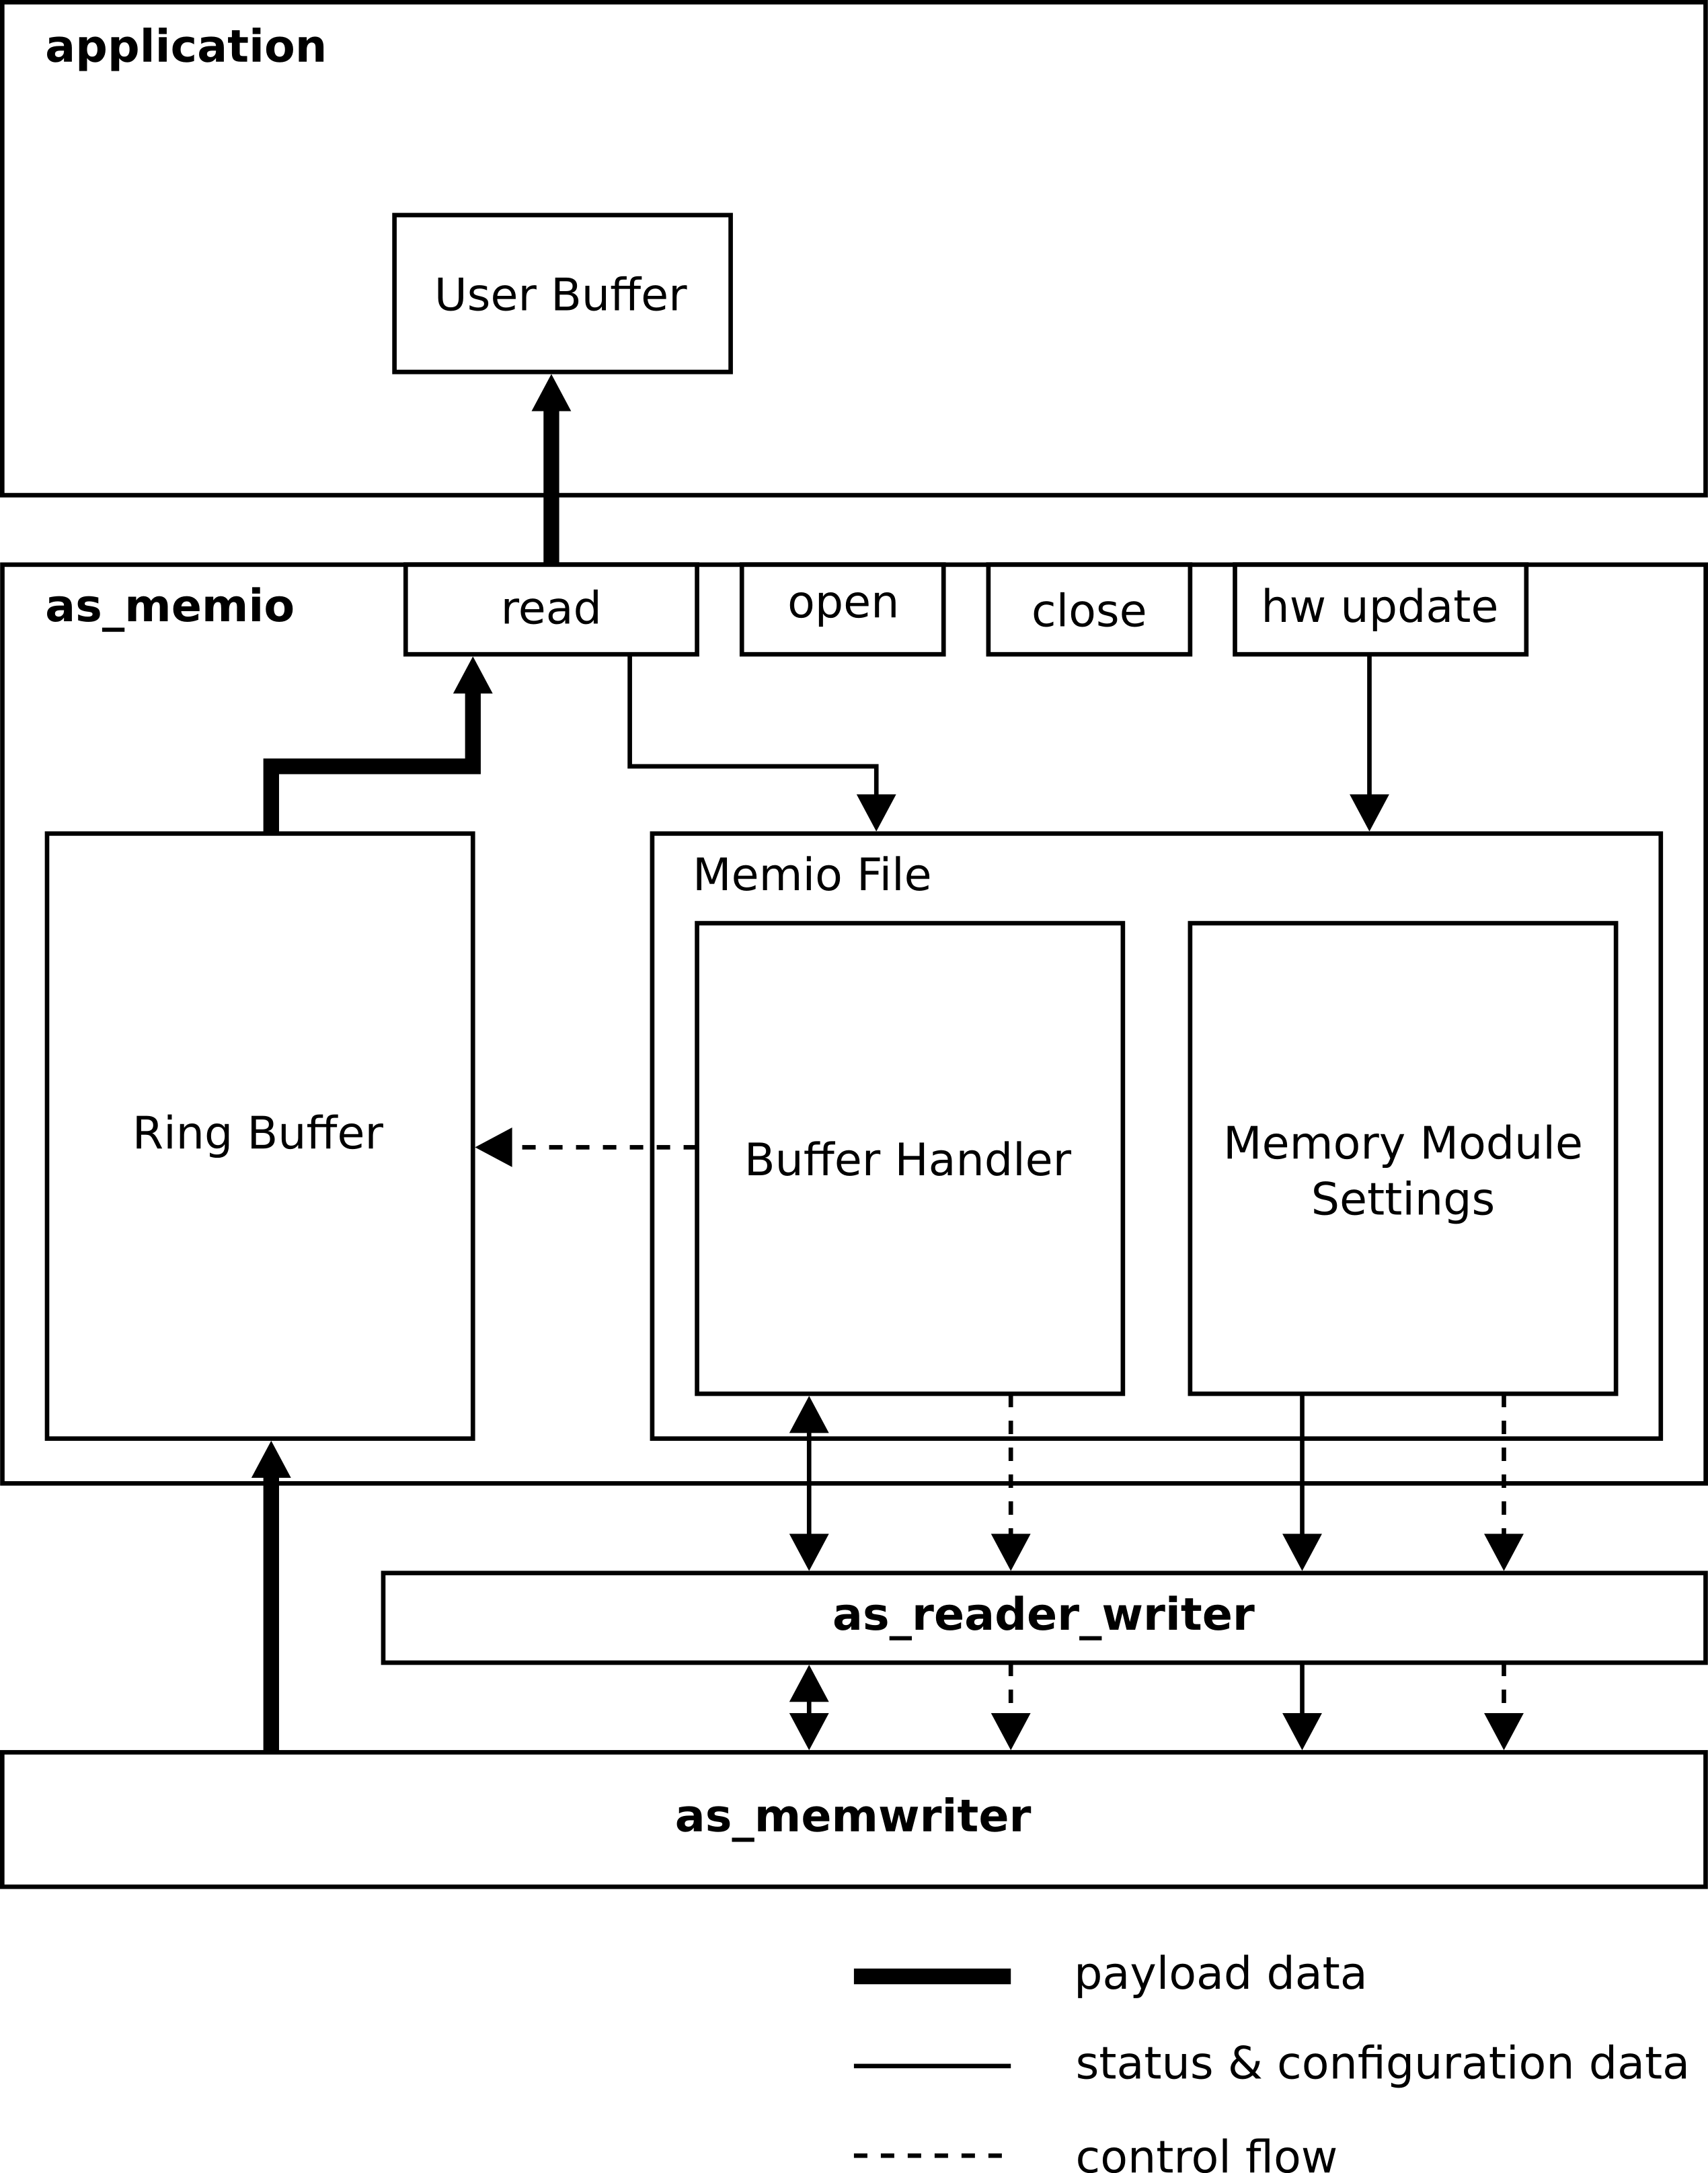
\includegraphics[width=0.6\linewidth,clip]{figs/memio.png}
    \caption{Architecture of the \texttt{as\_memio} module and its software/hardware interaction}
    \label{fig:memio}
\end{figure}

\subsubsection{Compile-Time Options}\label{ch:07-basic-modules-as_memio-options}
% buffer size in byte
% safety distance in byte (transfer size)
\begin{longtable}[ht]{|l|l|l|}
    \hline
    \multicolumn{1}{|c|}{\textbf{Name}} & \multicolumn{1}{c|}{\textbf{Range}} & \multicolumn{1}{c|}{\textbf{Description}}\\
    \hline
    
    \parbox{5cm}{\small{AS\_MEMIO\_DEFAULT\_}\\\small{INTERFACE\_WIDTH}} & Positive integer value & \parbox{5cm}{\ \\
        Sets the default bit width for ALL (!) memory module bus interfaces (usually 32 or 64 bit).\\
        This parameter is likely to be dropped in a future version of \texttt{as\_memio}.\\
    }\\
    \hline
    
    \parbox{5cm}{\small{AS\_MEMIO\_DEFAULT\_}\\\small{MAX\_BURST\_LENGTH}} & Positive integer value & \parbox{5cm}{\ \\
        Sets the default burst length in byte for ALL (!) memory modules (usually 256).\\
        This parameter is likely to be dropped in a future version of \texttt{as\_memio}.\\
    }\\
    \hline
    
    \parbox{5cm}{\small{AS\_MEMIO\_DEFAULT\_}\\\small{HW\_TRANSFER\_SIZE}} & Positive integer value & \parbox{5cm}{\ \\
        Sets the default \textit{transfer size} in byte for ALL (!) \texttt{as\_memio} modules.\\
        The \textit{transfer size} is the minimum \textit{section size} to be configured for the \texttt{as\_memwriter}.\\
        Prevents data loss at the \textit{FIFO Buffer} which may occur due to too small \textit{sections}.\\
    }\\
    \hline
    
    \parbox{5cm}{\small{AS\_MEMIO\_DEFAULT\_}\\\small{FIFO\_BUFFER\_SIZE}} & Positive integer value & \parbox{5cm}{\ \\
        Sets the default \textit{Ring Buffer} size in byte for ALL (!) \texttt{as\_memio} modules.\\
        Increasing the size allows the memory module to transfer more data for a single configuration.\\
    }\\
    \hline
    
\end{longtable}

\subsubsection{Register Space}

The module described does not contain any memory-mapped control or status registers, since it is a software module.

\subsubsection{Behavior}\label{ch:07-basic-modules-as_memio-behavior}

% open
In order to establish a connection between a memory module and \texttt{as\_memio}, its \textit{open} function has to be called, named \texttt{as\_memio\_open}.
Here, the address of the memory module has to be provided, which is internally used for calls to the functions of the \texttt{as\_reader\_writer} driver.
By providing the direction of the data flow via the \texttt{flags} parameter, either a \texttt{as\_memreader} or \texttt{as\_memwriter} is associated with the instance of \texttt{as\_memio}.
The \texttt{as\_memio} module is not able to determine the module type based on the address of the memory module.
Alternatively, a pointer to a configuration structure of the type \texttt{as\_memio\_config\_t} can be provided to overwrite the default settings for this \texttt{as\_memio} instance (see \ref{ch:07-basic-modules-as_memio-options}).
If a NULL pointer is provided, the default settings are used instead.
Within the \texttt{as\_memio\_open} function, the \textit{Ring Buffer} and \textit{Memio File} are allocated.
Subsequently, the static settings of the associated memory module are initialized, such as the \texttt{max burst length}.
Lastly, the memory module is reset and the pointer to the \textit{Memio File} is returned to the user for referencing to this instance of \texttt{as\_memio}, similar to a file pointer of the POSIX \textit{open} function.
The contents of the \textit{Memio File} are hidden from the user.

% read
The function \texttt{as\_memio\_read} is used for transferring data from hardware to software.
Next to the \textit{Memio File} pointer, a \textit{User Buffer} and the desired number of bytes have to be provided.
The requested number of bytes are copied to this buffer and therefore has to be of appropriate size.
First, the \texttt{as\_memio\_read} function is checks the current status of the \texttt{as\_memwriter} module.
The \texttt{current hw addr} is read, which determines the current location within the \textit{Ring Buffer}, where the \texttt{as\_memwriter} writes to.
Additionally, if the \texttt{pending go} bit field of the \texttt{control} register is not set, the next \textit{section} is programmed, as long as there is enough empty space within the \textit{Ring Buffer}.
All addresses up to \texttt{current hw addr} have been served by the hardware module.
The actual amount of data available in the \textit{Ring Buffer} is determined by using this address in combination with the last address copied to a \textit{User Buffer} for a previous call to \texttt{as\_memio\_read}.
Figure~\ref{fig:memio_buffer_read} shows how the available data within the \textit{Ring Buffer} is determined. 
The \texttt{current hw addr} is shown as \textit{hw} and the following address after the last copy process to the \textit{User Buffer} as \textit{sw}.
Both are represented within the \textit{Buffer Handler} of \texttt{as\_memio}.
If the number of bytes in the \textit{Ring Buffer} is not equal to the requested one, the smaller number of bytes is copied.
The address of \textit{sw} is increased for each copied byte to the \textit{User Buffer} throughout the lifetime of the \texttt{as\_memio} instance.
If either \textit{hw} or \textit{sw} exceeds the upper boundary of the \textit{Ring Buffer}, it is set to its start address again (bottom).
The \textit{Buffer Handler} prevents buffer over- and underflow due to one pointer overtaking the other.
After completing \texttt{as\_memio\_read}, the actual number of copied bytes is returned to the caller and the \textit{User Buffer} contains the data.

\begin{figure}[ht]
    \centering
    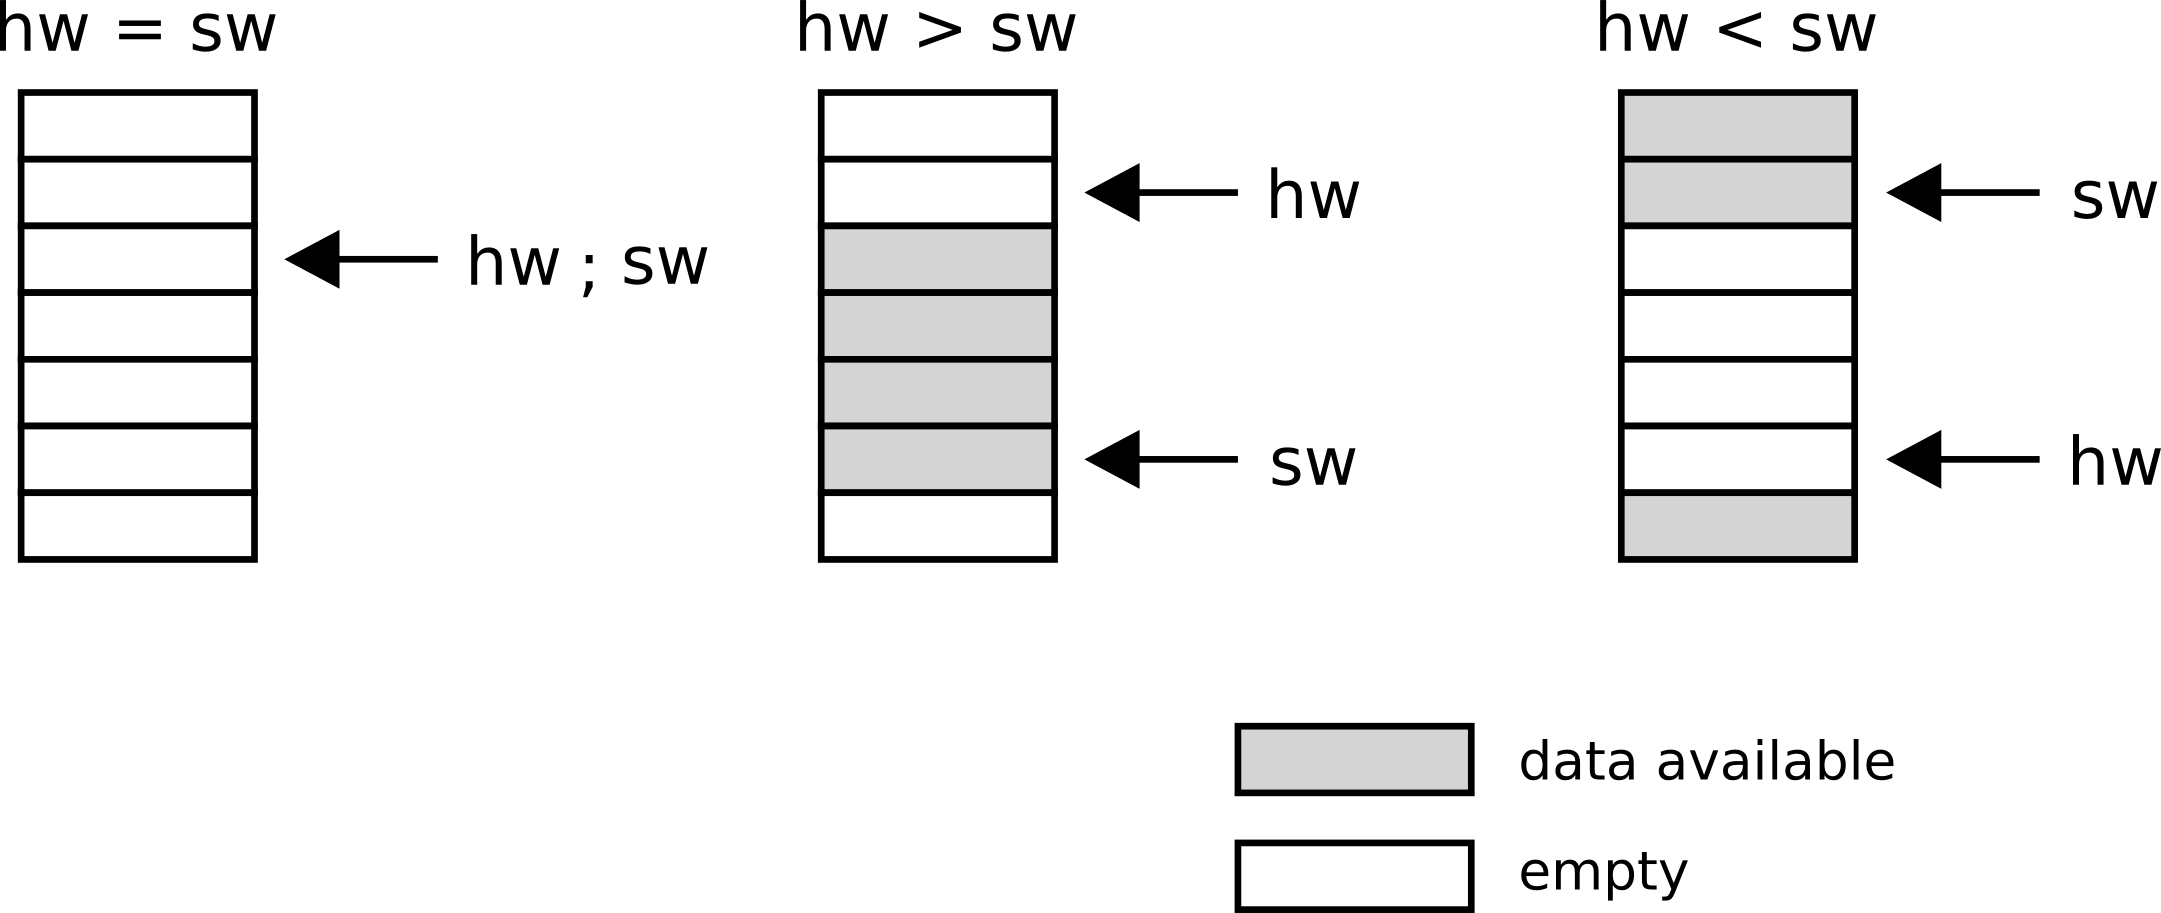
\includegraphics[width=0.6\linewidth,clip]{figs/memio_buffer_read.png}
    \caption{Determining the available amount of data within the \textit{Ring Buffer} for \texttt{as\_memio\_read}}
    \label{fig:memio_buffer_read}
\end{figure}

% write
The \texttt{as\_memio\_write} function operates in a similar way but data is copied from the \textit{User Buffer} to the empty slots of the \textit{Ring Buffer}.
Figure~\ref{fig:memio_buffer_write} shows how the available addresses within the \textit{Ring Buffer} are determined.
Since a \texttt{as\_memreader} is associated with this function it can only be configured once data is available in the \textit{Ring Buffer}.
Therefore, \texttt{current hw addr} is read after copying the data from the \textit{User Buffer} as well as programming the next \textit{section} in case the \texttt{pending go} field of the \texttt{control} register is not set.
Although \texttt{as\_memio} has been able to copy all data to the \textit{Ring Buffer}, the actual data transfer may not yet be completed after \texttt{as\_memio\_write} returns.

\begin{figure}[ht]
    \centering
    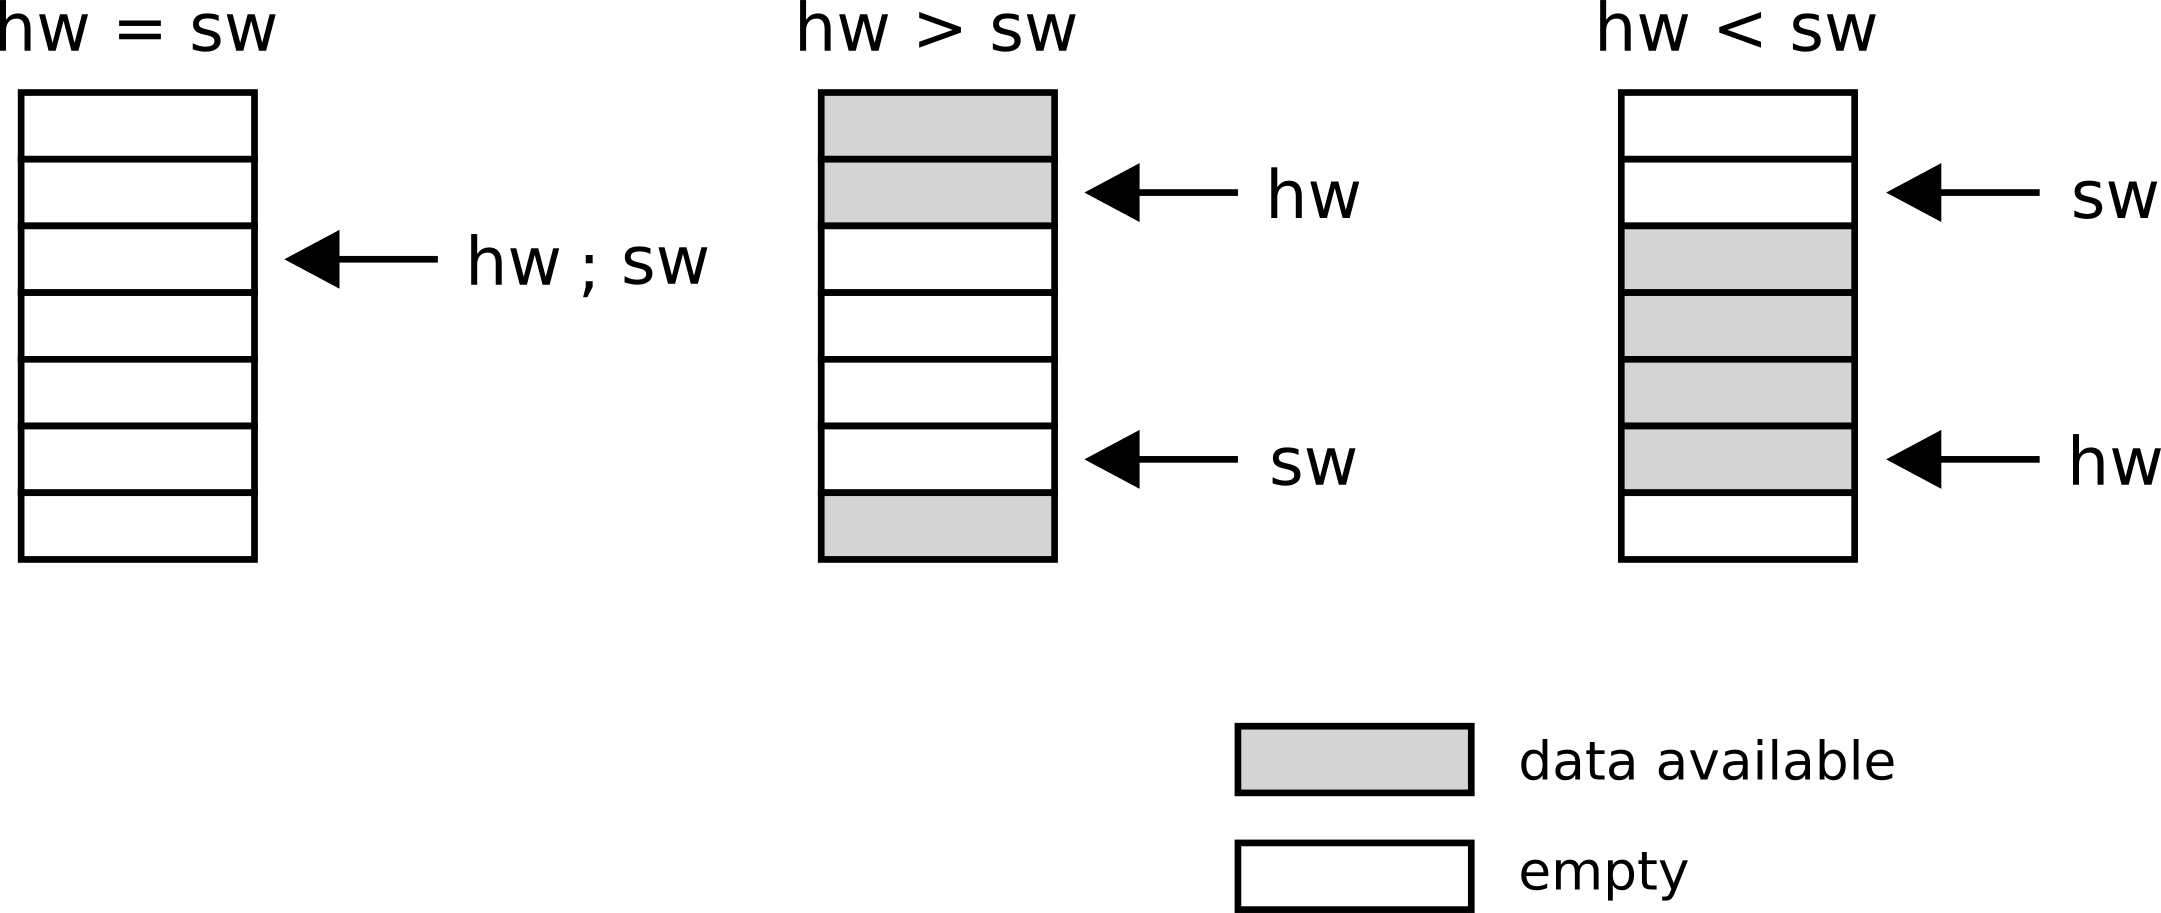
\includegraphics[width=0.6\linewidth,clip]{figs/memio_buffer_write.png}
    \caption{Determining the available amount of data within the \textit{Ring Buffer} for \texttt{as\_memio\_write}}
    \label{fig:memio_buffer_write}
\end{figure}

% hw update
The \texttt{as\_memio} module implicitly programs its associated memory module when calling either \texttt{as\_memio\_read} or \texttt{as\_memio\_write}.
Although sufficient in most cases, explicitly programming the memory module is required if the last data transfer between the \textit{Ring Buffer} and \textit{User Buffer} results in a boundary crossing by the hardware module.
Since the memory modules only support a single \textit{section} which has to consist of physically concurrent addresses, wrapping around the \textit{Ring Buffer} requires programming the memory modules twice.
This is shown in Figure~\ref{fig:memio_buffer_read} and~\ref{fig:memio_buffer_write} for "hw $>$ sw", where the first \textit{section} has to be programmed starting from \textit{hw} up to the end of the \textit{Ring Buffer} and the second on from the beginning.
The second \textit{section} can be programmed by using the \texttt{as\_memio\_hw\_update} function.
When the instance of \texttt{as\_memio} is associated with a \texttt{as\_memreader}, it prevents data from getting "stuck" in the \textit{Ring Buffer} which could cause the image processing chain to wait indefinitely for data to arrive.
For the \texttt{as\_memwriter}, it prevents a potential overflow of its \textit{FIFO Buffer} due to not being able to transfer the data to the \textit{Ring Buffer}.

% Transfer size
Although the \texttt{as\_memwriter} is able to request the preceding hardware module to suspend data transfers when its \textit{FIFO Buffer} is full, not all modules are able to suspend their transfers (e.g. camera).
For this reason, the \texttt{as\_memio} module uses a \textit{transfer size} when programming the \textit{section} size for the \texttt{as\_memwriter} to cater for continuous data streams.
The \textit{transfer size} is the minimum number of bytes which have to be transferred by the \texttt{as\_memwriter} to prevent overflows of its \textit{FIFO Buffer} due to setting up a too small \textit{section}.
This is mainly relevant when the \texttt{as\_memwriter} is about to cross the upper boundary of the \textit{Ring Buffer} of the \texttt{as\_memio} module.
Since two \textit{sections} have to be programmed when wrapping around the \textit{Ring Buffer}, the first one has to be big enough to give the software time to program the second one.
The \textit{FIFO Buffer} of the \texttt{as\_memwriter} must not overflow during this given time window.
The \textit{Ring Buffer} of \texttt{as\_memio} has to be a multiple of the \textit{transfer size}.

% close
The call to \texttt{as\_memio\_close} deletes a no longer required instance of the \texttt{as\_memio} module.
Here, the associated memory module is reset and all acquired resources are returned. 
Since the \textit{Memio File} no longer exists after this point, it can no longer be used. 

All calls to the functions of the \texttt{as\_memio} module are nonblocking and therefore return immediately even if the request could not be fulfilled.
This may require to call \texttt{as\_memio\_read} or \texttt{as\_memio\_write} more than once to transfer the desired number of bytes.



\subsubsection{Application Notes}
Figure~\ref{lst:memio_simple} shows the setup of the \texttt{as\_memio} module using default settings.

\begin{footnotesize}
    \lstset{style=CStyle, caption={Using \texttt{as\_memio} for transferring data from hardware to software}}
    \begin{lstlisting}[label=lst:memio_simple]
    
    #define IMAGE_RES           640*480
    int n;
    
    void *user_buffer = as_malloc(IMAGE_RES);
    
    /******* Setting up as_memio *******/
    
    struct as_memio_file_s *memio_read_fp = \
        as_memio_open(AS_ADDR(AS_MODULE_BASEREG_MEMWRITER_0), \
            NULL, O_WRONLY);
    
    
    /************** Data transfer **************/
    
    n = 0;
    
    while(n < IMAGE_RES) {
    n += as_memio_read(memio_read_fp, user_buffer+n, IMAGE_RES-n)
    }
    
    \end{lstlisting}
\end{footnotesize}



\clearpage
%%%%%%%%%%%%%%%%%%%%%%%%%%%%% Camera Modules %%%%%%%%%%%%%%%%%%%%%%%%%%%%%%%%
\section{Camera Interfaces}



\subsection{as\_picam}

\secauthor{Thomas Izycki}

The \texttt{as\_picam} module was developed in order to use a \textit{Raspberry Pi} camera v1.3 or v2.1 with an \asterics chain on a TE0726 Zynqberry\footnote{\url{https://shop.trenz-electronic.de/en/TE0726-03M-ZynqBerry-Module-with-Xilinx-Zynq-7010-in-Raspberry-Pi-Form-Faktor}}. It is operated in combination with the \texttt{video\_in} subsystem provided by \textit{Trenz Electronic GmbH}. The subsystem consists of several modules and interfaces the camera by implementing the CSI-2 specification. As long as the \textit{enable} signal is active, a continuous video stream is apllied to its AXI-Stream output with 8-bit per pixel in the ABGR format.
For further information on the \texttt{video\_in} subsystem refer to section \ref{sec:09-01-as_refdesign_zynqberry}.

\subsubsection{Module Description}

The \texttt{as\_picam} module serves as a link between the \texttt{video\_in} subsystem and the \asterics chain with image data being transmitted via AXI-Stream. A constant enable signal applied to the \texttt{video\_in} subsystem keeps the camera permanently in operation, generating a steady video stream. In addition the AXI-Stream's \textit{READY} signal is also kept high the entire time, meaning new data is accepted every clock cycle. For use within the ASTERICS chain the \texttt{as\_picam} module provides an \texttt{as\_stream} output interface. Figure \ref{07-as-picam-wave} shows the AXI-Stream input compared to the \texttt{as\_stream} output at the beginning of a new image frame, indicated by the \textit{start of frame} (SOF) signal.

\begin{figure}[htbp]
    \noindent \begin{centering}
    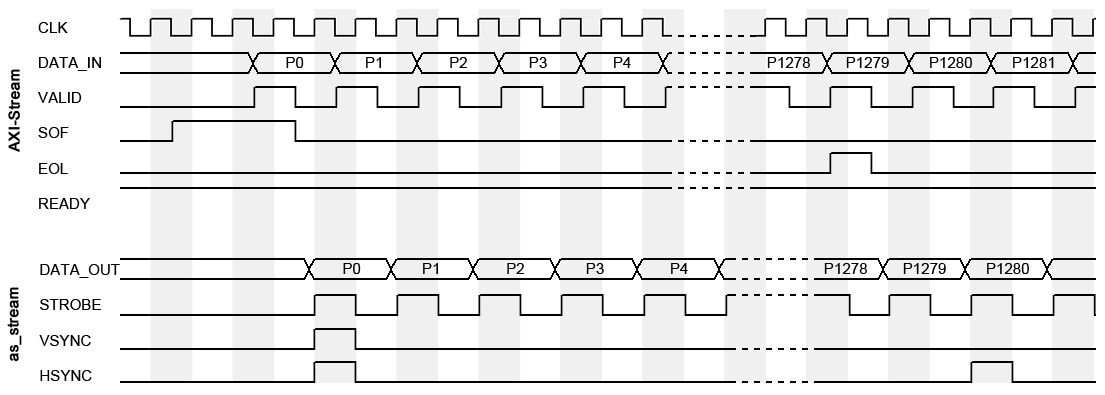
\includegraphics[width=\textwidth]{figs/07-as_picam_wave.png}
    \par\end{centering}
    \caption{Conversion of AXI-Stream to as\_stream}
    \label{07-as-picam-wave}
\end{figure}

In contrast to the \texttt{as\_stream} specification that needs the \textit{HSYNC} signal to be generated with the first pixel of every line, the AXI-Stream protocol defines the \textit{end of line} (EOL) signal occurring with the last pixel of a line.
Beside the AXI-Stream to \texttt{as\_stream} conversion the 32-bit BGRA image data is transformed into 8-bit grayscale.
\subsubsection{Register Space}

The module has one 32-bit wide combined status and control register depicted in Table \ref{07-as-picam-register}.

\begin{longtable}[htb]{|c|c|c|c|}
\hline
\textbf{Bit Name} & \textbf{Index} & \textbf{Access} & \textbf{Description} \\
\hline
\endhead

\texttt{Frame Done} & 0 & R &
\parbox{8,5cm}{ ~ \\ Frame completely transmitted. \\ ~  \small
This status bit is set by the hardware when the last pixel of an image has been transferred.
\vspace{0.3em} ~ } \\

\hline

\texttt{Data Enable} & 17 & W &
\parbox{8,5cm}{ ~ \\ Enables the video stream. \\ ~ \small
As soon as this bit is set, the camera images are output continously as grayscale images.
\vspace{0.3em} ~ } \\

\hline

\texttt{Enable Once} & 18 & W &
\parbox{8,5cm}{ ~ \\ Process one image. \\ ~  \small
Setting this bit has the effect that exactly one complete image is output as a grayscale image.
\vspace{0.3em} ~ } \\

\hline

\caption{Bit fields of the status and control register}
\label{07-as-picam-register}
\end{longtable}

\subsubsection{Software Driver}

The software driver serves two purposes. The first one is to initialize the \textit{Raspberry Pi} camera by configuring it via \textit{i2c}. Therefore the processing system's \textit{i2c} module is used and the corresponding setup is loaded into the camera's registers. However, only resolutions of 1280x720 pixels are supported. The distinction between the \textit{Raspberry Pi} camera v1.3 and 2.1 is made automatically.
The second purpose is to interface the hardware. Either the camera is set to a constant run mode, streaming the video data or every frame is triggered individually.



\clearpage
%%%%%%%%%%%%%%%%%%%%%%%%%%%%% Converters and Adapters %%%%%%%%%%%%%%%%%%%%%%%%%%%%%%%%
\section{Converters and Adapters}


\subsection{as\_collect}

\secauthor{Julian Sarcher, Alexander Zöllner}

\subsubsection{Brief Description}

The collect module collects smaller data words (e.g. 8 bit wide) until a certain bit width is reached. As the desired bit width is reached, the collect module forwards the larger data word. An example usage for this module is collecting 8-bit gray scale pixels for 32 or 64 bit memory bus accesses.

\subsubsection{Configuration Options}

\begin{tabular}{|c|c|c|}
    \hline
    \textbf{Name} & \textbf{Description} & \textbf{Range} \\ \hline
    
    % First tabular line / First Generic:
    DIN\_WIDTH & 
    \begin{tabular}{c} Data width of DATA\_IN \end{tabular} & 
    \begin{tabular}{c} Power of two $ \wedge $ \\ DIN\_WIDTH $<$ DOUT\_WIDTH \end{tabular}  
    \\ \hline
    
    % Second line / Second Generic:
    DOUT\_WIDTH & 
    \begin{tabular}{c} Data width of DATA\_OUT \end{tabular} & 
    \begin{tabular}{c} Power of two $ \wedge $ \\ DOUT\_WIDTH $<$ DIN\_WIDTH \end{tabular}  
    \\ \hline
\end{tabular}

\subsubsection{Register Space}

The module described does not contain any memory-mapped control or status registers.

\subsubsection{Resource Utilization}

%\begin{verbatim}
%[[
%
%TBD: Resource utilization obviously depends 
%on the generic adjusment. So far, there are no 
%experiments made for different generic adjustments.
%
%]]
%
%\end{verbatim}

\begin{tabular}{|c|c|c|c|c|}
    \hline
    DIN\_WIDTH & DOUT\_WIDTH & Slices & Block-RAM & DSP-Slices \\ \hline
    8 & 64 & 26 (0.2\%) & 0 (0.0\%) & (0.0\%) \\ \hline
\end{tabular}


%%%%%%%%%%%%%%%%%%%%%%%%%%%%%%%%%%%%%%%%%%%%%%%%%%%%%%%%% as_stream_adapter %%%%%%%%%%%%%%%%%%%%%%%%%%%%%%%%%%%%%%%%%%%%%%

\subsection{as\_stream\_adapter}

\secauthor{Philip Manke}

\subsubsection{Brief Description}

The module \texttt{as\_stream\_adapter} is capable of adjusting the bit width of an \texttt{as\_stream}'s data signal without modifying the data contents.
Almost arbitrary combinations of bit width conversions are possible.
The module can both collect data to implement a narrow to wide conversion and disperse data to implement a wide to narrow conversion.
Furthermore, the bit widths converted between do not have to be multiples of each other.

Valid conversions are, for example:
\begin{itemize}
\setlength\itemsep{-0.2em}
\item 8 to 32 bits
\item 32 to 8 bits
\item 32 to 24 bits
\item 8 to 1 bit
\item 17 to 32 bits
\end{itemize}
 
\textit{Note:}
The module's FPGA resource requirements scale by the least common multiple between the configured input and output bit widths.


\subsubsection{Configuration Options / Generics}

\begin{tabular}{|c|c|c|}
    \hline
    \textbf{Name} & \textbf{Range} & \textbf{Description} \\ \hline
    
    % First tabular line / First Generic:
    DIN\_WIDTH & 
    \begin{tabular}{c} \(]0,+\infty]\) \end{tabular} & 
    \begin{tabular}{c} Bit width of \texttt{data\_in} \end{tabular}
    \\ \hline
    
    % Second line / Second Generic:
    DOUT\_WIDTH & 
    \begin{tabular}{c} \(]0,+\infty]\) \end{tabular} & 
    \begin{tabular}{c} Bit width of \texttt{data\_out} to adapt to \end{tabular}  
    \\ \hline
    
    \parbox{4.5cm}{GENERATE\_STROBE\_\\COUNTERS} & 
    \begin{tabular}{c} \texttt{true, false} \end{tabular} &
    \begin{tabular}{c} \parbox{7cm}{\ \\ Wether to add two registers with counters for incoming and outgoing strobe signals.  \vspace{0.3em} } \end{tabular}  
    \\ \hline
\end{tabular}


\subsubsection{Register Space}

This module utilizes four 32 bit wide registers the contents and functionality of which are described in the following tables.

\begin{longtable}[ht]{|l|c|c|l|}
    \hline
    \multicolumn{1}{|c|}{\textbf{Name}} & \multicolumn{1}{c|}{\textbf{Offset}} & \multicolumn{1}{c|}{\textbf{Access}} & \multicolumn{1}{c|}{\textbf{Description}}\\
    \hline
    
    \texttt{state} & \texttt{0x0} & R & \parbox{8.5cm}{\ \\
        Status bits and information.\vspace{0.3em}
    }\\
    \hline
    
    \texttt{control} & \texttt{0x1} & W & \parbox{8.5cm}{\ \\
        Control bits for software control.\vspace{0.3em}
    }\\
    \hline
    
    \parbox{3.5cm}{\texttt{incoming strobe counter}} & \texttt{0x2} & R & \parbox{8.5cm}{\ \\
        Contains the number of counted incoming strobes if \texttt{GENERATE\_STROBE\_COUNTERS} is set to \texttt{true}.\vspace{0.3em}
    }\\
    \hline
    
    \parbox{3.5cm}{\texttt{outgoing strobe counter}} & \texttt{0x3} & R & \parbox{8.5cm}{\ \\
        Contains the number of counted outgoing (generated) strobes if \texttt{GENERATE\_STROBE\_COUNTERS} is set to \texttt{true}.\vspace{0.3em}
    }\\
    \hline
    \caption{Register overview of the \texttt{as\_stream\_adapter} module.}
\end{longtable}



\begin{longtable}[ht]{|l|c|c|l|}
    \hline
    \multicolumn{1}{|c|}{\textbf{Bit Name}} & \multicolumn{1}{c|}{\textbf{Index}} & \multicolumn{1}{c|}{\textbf{Access}} & \multicolumn{1}{c|}{\textbf{Description}}\\
    \hline
    
    \texttt{buffer full} & 0 & R & \parbox{8.5cm}{\ \\
        If '1', indicates that the module's internal data buffer is full and it is sending data or waiting to send data.\vspace{0.3em}
    }\\
    \hline
    
    \texttt{buffer empty} & 1 & R & \parbox{8.5cm}{\ \\
        If '1', indicates that no more data will be send by this module until new data is received.\vspace{0.3em}
    }\\
    \hline
    
    \texttt{unused} & 2 .. 6 & R & \parbox{8.5cm}{\ \\
        Not used, always returns 0.\vspace{0.3em}
    }\\
    \hline
    
    \parbox{3.5cm}{ \texttt{strobe counters enabled}} & 7 & R & \parbox{8.5cm}{\ \\
        '1' if the module is configured with strobe counters (\texttt{GENERATE\_STROBE\_COUNTERS} is set to \texttt{true}).\vspace{0.3em}
    }\\
    \hline
    
    \texttt{buffer size} & 8 .. 31 & R & \parbox{8.5cm}{\ \\
        Set to the size of the internal data buffer in bits. Should equal the least common multiple of \texttt{DIN\_WIDTH} and \texttt{DOUT\_WIDTH}.\vspace{0.3em}
    }\\
    \hline
    
    \caption{Bit field overview of the state register of \texttt{as\_stream\_adapter}.}
\end{longtable}


\begin{longtable}[ht]{|l|c|c|l|}
    \hline
    \multicolumn{1}{|c|}{\textbf{Bit Name}} & \multicolumn{1}{c|}{\textbf{Index}} & \multicolumn{1}{c|}{\textbf{Access}} & \multicolumn{1}{c|}{\textbf{Description}}\\
    \hline
    
    \texttt{reset} & 0 & W & \parbox{9cm}{\ \\
        Resets the module's state and clears the internal data buffer when set to '1'. Must also be unset by software.\vspace{0.3em}
    }\\
    \hline
    
    \texttt{reset counters} & 1 & W & \parbox{9cm}{\ \\
        Resets the module's strobe counters when set to '1'. Must also be unset by software.\vspace{0.3em}
    }\\
    \hline
    
    \caption{Bit field overview of the control register of \texttt{as\_stream\_adapter}.}
\end{longtable}


\subsubsection{Behavior}

This module can operate in three different modes defined by the values of \texttt{DIN\_WIDTH} and \texttt{DOUT\_WIDTH}:

\begin{itemize}
\setlength{\itemsep}{-0.2em}
\item \textbf{Collection mode} (\texttt{DIN\_WIDTH > DOUT\_WIDTH}): The bit width of the data signal is increased.
\item \textbf{Dispersion mode} (\texttt{DIN\_WIDTH < DOUT\_WIDTH}): The bit width of the data signal is decreased.
\item \textbf{Pass-through mode} (\texttt{DIN\_WIDTH = DOUT\_WIDTH}): The bit width of the data signal is not modified.
\end{itemize}

In general, this module delays the data signal by at one clock cycle.
The data signal will be delayed more when \texttt{as\_stream\_adapter} is operating in collect mode.
When enough data has been accumulated in the internal buffer to allow for a data word to be output, this will happen one clock cycle after the last data word was received.
Any synchronization signals (\texttt{vsync, hsync,} etc.) received while data is collected will be output with the next data word.


In disperse mode, the module will emit a stall signal when the internal buffer is full.
A clock cycle before the final data word is send by the module, it will stop emitting the stall signal.
This gives the preceding modules a relatively short notice to start sending more data.
This may result in an underutilization of the following modules, as any delay longer than one clock cycle will result in a delay at the module's output.
Any synchronization signals (\texttt{vsync, hsync,} etc.) received with an incoming data word are output once with the first data word that contains part of the received data word.


Pass-through mode can make sense when used in conjunction with the strobe counter feature built-in to the module.
Otherwise this mode does not provide any functionality, except for a one clock cycle delay.



\clearpage
%%%%%%%%%%%%%%%%%%%%%%%%%%%%% Image Processing %%%%%%%%%%%%%%%%%%%%%%%%%%%%%%%%
\section{Image Processing Modules}



\construction{section}


\clearpage
%%%%%%%%%%%%%%%%%%%%%%%%%%%%% Bus and Protocol Modules %%%%%%%%%%%%%%%%%%%%%%%%%%%%%%%%
\section{Protocol and Bus Modules}

%%%%%%%%%%%%%%%%%%%%%%%%%%%%%%%%%%%%%%%%%%%%%%%%%%%%%%%%%%%%%%%%%%%%%%%%%%%%%%
%%
%% This file is part of the ASTERICS Framework. 
%%
%% Copyright (C) Hochschule Augsburg, University of Applied Sciences
%% Efficient Embedded Systems Group
%%
%% Author(s): Philip Manke <philip.manke@hs-augsburg.de>
%%
%%%%%%%%%%%%%%%%%%%%%%%%%%%%%%%%%%%%%%%%%%%%%%%%%%%%%%%%%%%%%%%%%%%%%%%%%%%%%%





%%%%%%%%%%%%%%%%%%%%%%%%%%%%% 7.5. i2c Master %%%%%%%%%%%%%%%%%%%%%%%%%%%%%%%%


\subsection{\textit{i2c} Bus Master} 
\label{ch:07-05-modules-i2c}
\secauthor{Philip Manke}

This section describes the module \texttt{as\_iic} in detail.
\texttt{as\_iic} implements a simple \textit{i2c} master with relatively limited functionality.


\subsubsection{General Overview of Features and Limitations}

The entire module was developed with a mindset of keeping the hardware small and adding only the most important features. Its primary use-case is configuring the cameras that are used with \asterics.

Figure \ref{07-05-as-iic-overview} gives a general overview of the ports of the module. 

\begin{figure}[htbp]
\noindent \begin{centering}
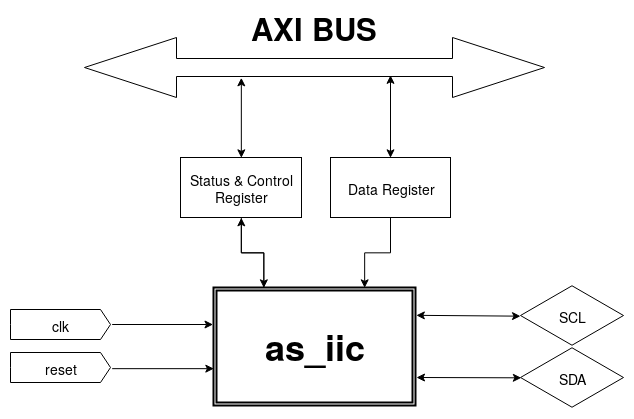
\includegraphics[width=\textwidth]{figs/07-05-as-iic-module-overview}
\par\end{centering}
\caption{Interfaces of the \texttt{as\_iic} hardware module}
\label{07-05-as-iic-overview}
\end{figure}

The following features are supported:

\begin{itemize}
	\item \textit{standard} and \textit{fast mode} \textit{i2c}.
	\item Variable bus clock (configurable via software) of frequencies between 10 kHz to 1 MHz
	\item Clock stretching
	\item 7 bit addressing
	\item Multi-byte transactions
	\item Master-acknowledge
\end{itemize}

\bigskip

The modules limitations are:

\begin{itemize}
	\item Only 8 bit addressing.
	\item No arbitration of any kind. Therefore, multi-master configurations are not supported.
	\item No faster modes of operation than Fast Mode.
	\item No interrupt support. The driver utilizes polling.
	\item No buffering of data. The driver has to transfer each byte sequentially.
\end{itemize}

10 bit addressing is possible with the current hardware, though it hasn't been implemented by the driver.

\subsubsection{The Hardware}

The hardware core consists of two state machines: one handles the generation of the bus clock (SCL) and the other controls the data signal (SDA) and the behaviour of the entire module.

\subsubsection*{The interfaces of \texttt{as\_iic}}

The \texttt{as\_iic} module requires two 32 bit slave registers on an AXI-Slave bus.
The first register is a combined status and control register, which also transfers the data received from the \textit{i2c} slave. 
The second register is read-only for the \texttt{as\_iic} hardware and is used to transfer the data to send to the \textit{i2c} bus and for configuring the \textit{i2c} bus clock frequency.

The status and control register is provided as three 16 bit registers for the status bits, the control bits and a special control-reset register respectively.
The control-reset register allows the AXI-Bus to reset control bits by itself.
If a bit in the control-reset register goes high, the respective bit in the control register is automatically set to low.
Table \ref{07-05-as-iic-registers} gives an overview of the registers of \texttt{as\_iic}.

\begin{longtable}[htb]{|c|c|c|c|}
\hline 
\textbf{Register Name} & \textbf{Access} & \textbf{Offset} & \textbf{Description} \\
\hline
\endhead

\texttt{Status \& Control Register} & RW & 1 &
\parbox{7cm}{ ~ \\ Status and control register for the hardware \\ ~ \\ \small
Half of this register reports the current status of the hardware module of \texttt{as\_iis} to the software. It is also used to transfer bytes, received from slaves on the \textit{i2c} bus, to the software.
The other half is used to control the hardware.
\\ ~ } \\

\hline 

\texttt{Data Register} & W & 0 &
\parbox{7cm}{ ~ \\ Data register for the hardware \\ ~ \\ \small
This register is used to control the hardware module.
Transactions can be initiated, stopped and modified, using bits of this register.
It also contains a soft reset bit.
\\ ~ } \\

\hline 

\caption{The registers of \texttt{as\_iic}}
\label{07-05-as-iic-registers}
\end{longtable}


The tables \ref{07-05-as-iic-control-bits} and \ref{07-05-as-iic-status-bits} explain the purpose of each control and status bit in more detail.

\begin{longtable}[htb]{|c|c|c|c|}
\hline 
\textbf{Bit Name} & \textbf{Access} & \textbf{Index} & \textbf{Description} \\
\hline
\endhead

\texttt{Start/Continue} & W & 0 &
\parbox{9cm}{ ~ \\ Start or continue a transaction. \\ ~ \small
This control bit is used to initiate a transaction from the ready state or continue a transaction for another byte after sending or checking for an acknowledge.
This bit is reset after sending/receiving a byte to/from the \textit{i2c} bus.
\vspace{0.3em} } \\

\hline 

\texttt{Stop} & W & 1 &
\parbox{9cm}{ ~ \\ Stop a transaction. \\ ~ \small
This control bit overwrites the Start/Continue bit and explicitly stops the current transaction after the next acknowledge or after the start bit.
This bit is reset when the hardware is in the ready state.
\vspace{0.3em} } \\

\hline 

\texttt{Read/Write} & W & 2 &
\parbox{9cm}{ ~ \\ Choose to write or read the next byte. \\ ~ \small
This bit toggles between writing a data byte onto the bus or reading a data byte from the bus.
It is sampled after checking for or sending an acknowledge.
This bit is only reset after stopping a transaction.
The default value is '0' (\^= write).
\vspace{0.3em} } \\

\hline

\texttt{Reset} & W & 3 &
\parbox{9cm}{ ~ \\ Completely reset the hardware. \\ ~ \small
This bit acts just like a hard reset for the \texttt{as\_iic} module.
The hardware will enter the ready state again after just a few clock cycles.
This bit is reset immediately.
\vspace{0.3em} } \\

\hline

\texttt{Data Ready} & W & 4 &
\parbox{9cm}{ ~ \\ Signal the hardware to continue. \\ ~ \small
This bit operates in conjunction with the status bit "Waiting SW".
When that status bit is set, the hardware is waiting for the software to finish setting up the data register for the next data byte or finish reading from the status register.
When the software is done, it needs to set this control bit.
The hardware will then continue with the transaction.
This bit is reset immediately.
\vspace{0.3em} } \\

\hline

\texttt{Ack Mod} & W & 5 &
\parbox{9cm}{ ~ \\ Send a master acknowledge. \\ ~ \small
This bit's only purpose is to tell the hardware to send an acknowledge after sending the \textit{i2c} slave address.
It is reset after sending/receiving a data byte.
\vspace{0.3em} } \\

\hline

\caption{Bit fields of the control register}
\label{07-05-as-iic-control-bits}
\end{longtable}

\begin{longtable}[htb]{|c|c|c|c|}
\hline 
\textbf{Bit Name} & \textbf{Access} & \textbf{Bit} & \textbf{Description} \\
\hline
\endhead


\texttt{IIC Ready} & R & 0 &
\parbox{8,5cm}{ ~ \\ The module's hardware is ready. \\ ~ \\ \small
This status bit is only set when the hardware is in the ready state.
\\ ~ } \\

\hline

\texttt{IO Ready} & R & 1 &
\parbox{8,5cm}{ ~ \\ The AXI Slave Registers are safe to read/write. \\ ~ \\ \small
When this status bit is set, the hardware is currently not reading/writing from/to the data byte parts of the AXI Slave registers, meaning that IO operations are allowed and safe.
\\ ~ } \\

\hline

\texttt{Bus Active} & R & 2 &
\parbox{8,5cm}{ ~ \\ This module is active on the \textit{i2c} bus. \\ ~ \\ \small
This status bit is always set when the \texttt{as\_iic} module is actively setting the SDA signal of the \textit{i2c} bus.
\\ ~ } \\

\hline

\texttt{Ack Rec} & R & 3 &
\parbox{8,5cm}{ ~ \\ Acknowledgement was received. \\ ~ \\ \small
This bit is set after checking for an acknowledgement bit from the slave after sending a data byte to the \textit{i2c} bus.
It should only be sampled after a write transaction as the value is only valid then.
Also note that this bit can only report on the state of the acknowledgement from the previous data byte.
It is reset just before checking for an acknowledge bit or when starting a new transaction.
\\ ~ } \\

\hline

\texttt{Stalled} & R & 4 &
\parbox{8,5cm}{ ~ \\ Clock stretching is detected. \\ ~ \\ \small
This bit is set every time clock stretching is detected.
Note that it is accurate to within a single system clock cycle.
The bit is reset immediately after the slave releases SCL.
\\ ~ } \\

\hline

\texttt{Waiting SW} & R & 5 &
\parbox{8,5cm}{ ~ \\ The hardware is waiting for the software. \\ ~ \\ \small
This bit is working in conjunction with the control bit "Data Ready".
When this bit is set, the hardware is waiting on the control bit "Data Ready" to be set by the software.
The hardware will always wait after sending/receiving a byte, before sending/checking for an acknowledge.
This allows the software to finish tasks like reading the last received data byte and writing the next data byte to be send.
This bit is immediately reset after the software sets "Data Ready".
\\ ~ } \\

\hline

\textit{Unused} & R & 6 - 7 &
\parbox{8,5cm}{ ~ \\ Unused \\ ~ \\ \small
\\ ~ } \\

\hline

\texttt{Data RX} & R & 8 - 15 &
\parbox{8,5cm}{ ~ \\ Data received from the bus \\ ~ \\ \small
This part of the status register is used by the hardware to transfer data received from slave devices on the bus to the software.
\\ ~ } \\

\hline


\caption{Bit fields of the status register}
\label{07-05-as-iic-status-bits}
\end{longtable}

\begin{longtable}[htb]{|c|c|c|c|}
\hline 
\textbf{Bit Name} & \textbf{Access} & \textbf{Bit} & \textbf{Description} \\
\hline
\endhead

\texttt{SCL\_DIV} & W & 0 - 23 &
\parbox{8,5cm}{ ~ \\ SCL counter compare value \\ ~ \\ \small
This value is used to reset the SCL counter, which is used to generate the \textit{i2c} bus frequency.
\\ ~ } \\

\hline 

\texttt{Data TX} & W & 24 - 31 &
\parbox{8,5cm}{ ~ \\ Data to send to the \textit{i2c} bus \\ ~ \\ \small
This part of the data register is used to transfer the bytes for the hardware to send on the bus.
\\ ~ } \\

\hline 

\caption{Bit fields of the data register}
\label{07-05-as-iic-data-register}
\end{longtable}

Besides the registers, there are the clock and hardware reset signals that go into the module and the SCL and SDA signals for the \textit{i2c} bus, which are "inout" signals, driven by the module using tristate drivers.
These signals should be connected to the outside using GPIO Pins connected to the \textit{i2c} devices, you wish to communicate with.
Though not intended, an internal \textit{i2c} bus could be configured just the same.

\subsubsection*{Generation of the SCL signal}

The data width used to configure the frequency for SCL differs, depending on the hardware configuration. It is always equal to the value of the "SCL\_DIV\_REGISTER\_WIDTH" generic, configurable before synthesis.
The data is little endian.

"SCL\_DIV\_REGISTER\_WIDTH", the modules only generic, sets the size of the counter that is used to detect when to switch the SCL signal. Therefore a wider counter allows for lower frequencies on the bus.
Also: With higher system clock frequencies a wider SCL DIV counter might be necessary to achieve the desired \textit{i2c} bus clock frequency.

The value used to configure the counter compare value in the data register (SCL\_DIV), is calculated as follows:

\[RegisterValue = (SystemFrequency / (4 * DesiredBusFrequency)) - 2 \]

With that, the ideal value for the "SCL\_DIV\_REGISTER\_WIDTH" generic is:

\[\log_{2}(RegisterValue)\]

Where the \textit{SystemFrequency} is the frequency of the clock driving the \texttt{as\_iic} module, \textit{DesiredBusFrequency} is the desired frequency of the SCL signal on the \textit{i2c} bus and \textit{RegisterValue} is the value to set the "Frequency for SCL" part of the data register to.\\
Note that the practical minimum value for the register value is 3.
This will run the hardware as fast as possible.

A state machine in conjunction with the aforementioned counter is used to generate the SCL clock signal. Every time the counter reaches the compare value configured via the data register, it is reset and a separate modulo 4 counter is incremented. Bit 1 of this smaller counter corresponds to the state of the SCL signal.
This also means that every time bit 0 of this smaller counter changes, one quarter of the bus clock period has passed.
This is an important signal for many parts of the hardware, as it changes exactly between and on the edges of the SCL clock signal.
Figure \ref{07-05-as-iic-scl-generation} shows a simplified diagram of the counters involved in generating the SCL signal.

\begin{figure}[htbp]
\noindent \begin{centering}
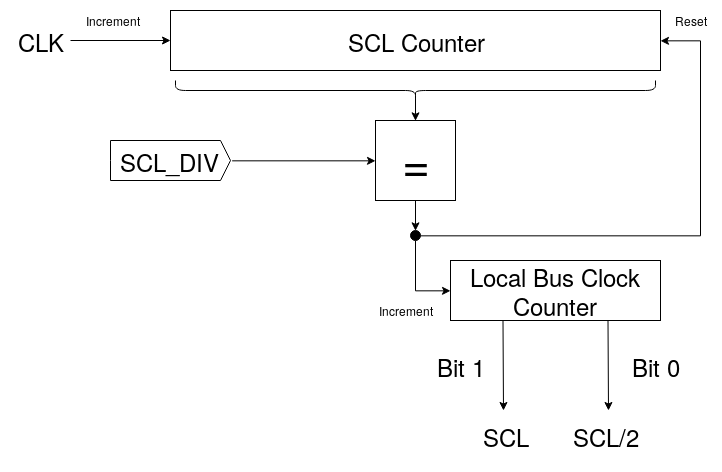
\includegraphics[width=\textwidth]{figs/07-05-as-iic-scl-generation}
\par\end{centering}
\caption{The counters generating the SCL Signal in \texttt{as\_iic}}
\label{07-05-as-iic-scl-generation}
\end{figure}

The state machine controls the counters and sets the SCL signal according to the mod 4 counter's state.
The "mod 4 counter" is also called \textit{local bus clock} or \textit{local bus clock counter} in hardware and in the graphic.
It also sets the "stalled" status signal, whenever clock stretching is detected.
This is done by monitoring the SCL bus signal and comparing it to the internal SCL signal (\textit{lbclk}).
If the signals differ from each other, another device on the \textit{i2c} bus is interfering with the clock signal (\^= "clock stretching").


\subsubsection*{The SDA state machine}

\begin{figure}[htbp]
\noindent \begin{centering}
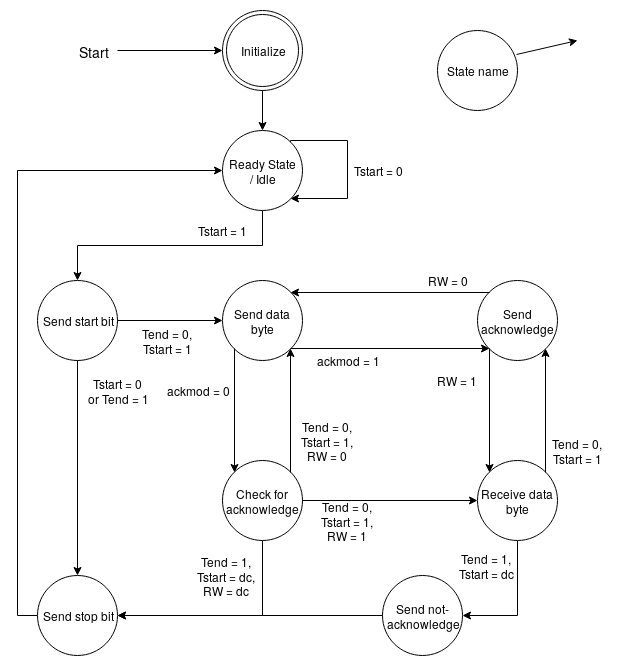
\includegraphics[width=\textwidth]{figs/07-05-as-iic-statemachine}
\par\end{centering}
\caption{Visualization of the SDA state machine in \texttt{as\_iic}}
\label{07-05-as-iic-states}
\end{figure}

This second larger state machine is used to control the SDA signal, manage the communication with the software via the AXI-Bus and manage the SCL state machine.\\
The states of this state machine can be grouped to correspond to different sections of the \textit{i2c} protocol, as seen in figure \ref{07-05-as-iic-states}.

The state machine oftentimes uses the \textit{i2c} bus signals SDA and SCL as parameters.
When it does that, these signals are not the internal signals, but are read directly from the bus, to make sure that clock stretching is always recognized.\\
When setting or sampling the SDA signal while sending or receiving a data byte, bit 0 from the \textit{local bus clock counter} (\textit{lbclk\_half}) is used as the trigger.
When this bit of the counter changes, exactly one quarter of the SCL clock period has passed, meaning that this is exactly in between two SCL clock edges. This guards against possible timing violations.

\subsubsection*{The "Master Acknowledge"}

A non-standard feature supported by this \textit{i2c} master implementation is the \textit{Master-Acknowledge}. After the slave address has been sent to the bus, the master is able to send an acknowledge bit by itself.
This behaviour is controlled by the software through the \texttt{ack\_mod} control bit. 
Some driver functions, like \texttt{set\_regpointer}, use this functionality and some functions take an additional parameter, the \texttt{modifier} byte, which can enable this and other functionality.

\subsubsection*{How to connect a hardware module to the \textit{i2c} bus} \label{07-05-as-iic-connect-devices}

As mentioned before the \textit{i2c} bus consists of just two signals/wires: SCL and SDA.
To connect a new slave device to the bus, these two wires of the \texttt{as\_iic} master need to be connected to the appropriate wires of the slave.
The SCL wires are connected together and the SDA wires are connected together.\\
The \textit{i2c} bus requires that each signal has a pull-up resistor connected to it.
This requires a resistor of between 1 kilo ohm and 10 kilo ohm to be connected to the signal and the supply voltage (usually 3.3 Volts) for both signals.

Possible problems with the \textit{i2c} bus include:

\begin{itemize}
	\item Multiple pull-up resistors present per signal
	\item Capacitance between the signals and ground is too high
	\item Interference from other signals
\end{itemize}

For more in-depth knowledge on the design of the hardware, consider looking through the VHDL source files of \texttt{as\_iic} available in \texttt{"modules/as\_iic/hardware/"}.

\subsubsection*{Waveform examples}

This section will further explain the \textit{i2c} protocol, using some waveform examples.\\
Figure \ref{07-05-as-iic-wave-write} shows some signals of a simulated \texttt{as\_iic} during a write operation.

\begin{figure}[htbp]
\noindent \begin{centering}
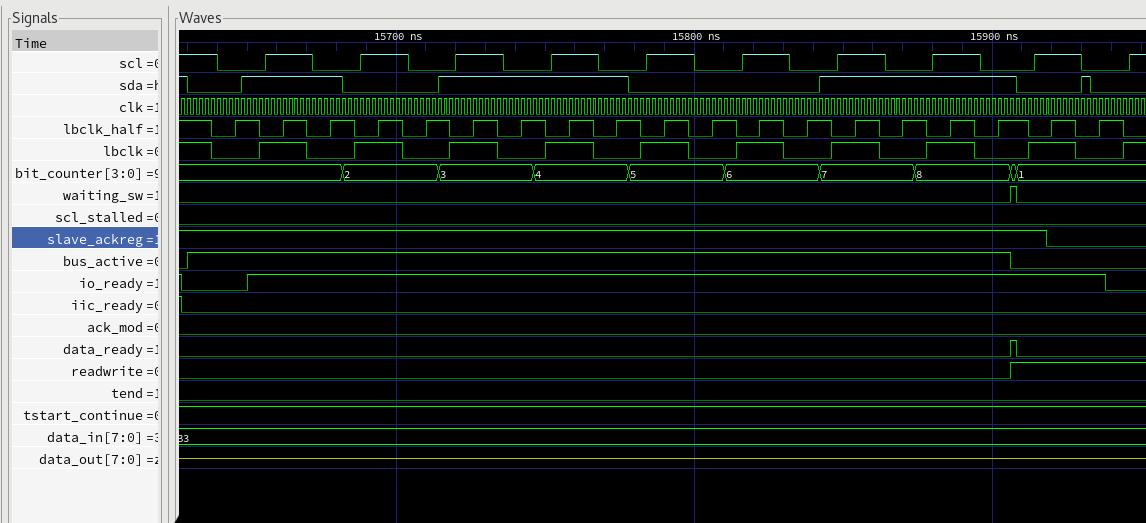
\includegraphics[width=\textwidth]{figs/07-05-as-iic-wave-write}
\par\end{centering}
\caption{\textit{i2c} read transaction as a waveform from a simulated \texttt{as\_iic} module}
\label{07-05-as-iic-wave-write}
\end{figure}

The first operation shown is the start bit, SDA going low while SCL is high followed by SCL going low while SDA is still low.
Following that, SDA may change while SCL is low and has to be valid when SCL goes high.\\
Furthermore some \texttt{as\_iic} specific relations can be demonstrated using this waveform.
The relationship between the system clock \texttt{clk}, the local bus clock counter, \texttt{lbclk} (\^= bit 1) and \texttt{lbclk\_half} (\^= bit 0), SCL and SDA where SCL is equal to \texttt{lbclk} but slightly delayed and SDA changes slightly after \texttt{lbclk\_half} goes high.

Figure \ref{07-05-as-iic-wave-read} shows a read transaction from the same simulated module.

\begin{figure}[htbp]
\noindent \begin{centering}
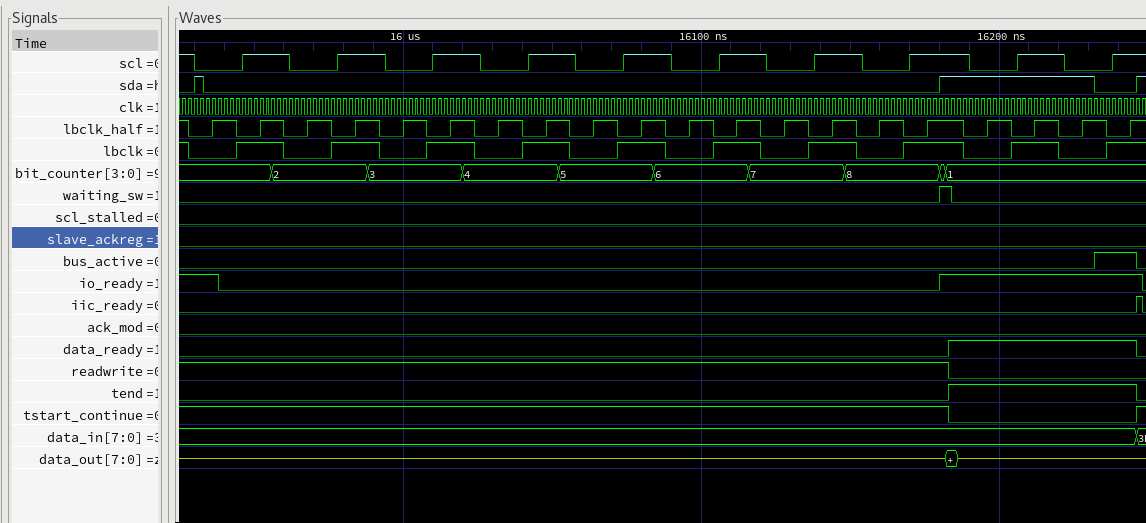
\includegraphics[width=\textwidth]{figs/07-05-as-iic-wave-read}
\par\end{centering}
\caption{\textit{i2c} write transaction as a waveform from a simulated \texttt{as\_iic} module}
\label{07-05-as-iic-wave-read}
\end{figure}

Finally figure \ref{07-05-as-iic-wave-real} shows a complete read transaction and write transaction captured using a logic analyzer using real hardware.
In this figure the start bits are marked by a green circle and the stop bits by a red circle.
Every transferred bit is marked by a small arrow on the edge of SCL going high, with the clock cycle for the acknowledge lacking this arrow.

\begin{figure}[htbp]
\noindent \begin{centering}
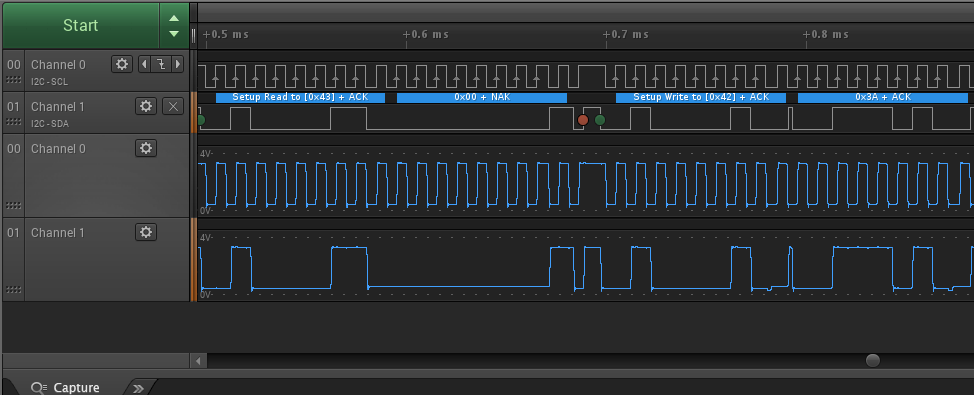
\includegraphics[width=\textwidth]{figs/07-05-as-iic-wave-real}
\par\end{centering}
\caption{Waveform captured using a logic analyzer from the \texttt{as\_iic} module}
\label{07-05-as-iic-wave-real}
\end{figure}

\subsubsection{The Software Driver}

The driver's low level functions are built to act as a modular system.
A few low level functions can be put together to a sequence, which can act as any possible \textit{i2c} transaction the hardware supports.
This means that less knowledge of this particular hard- and software implementation is required to expand the drivers functionality.
All of the lower level functions reference "transactions". This refers to all the actions between and including the start bit and the stop bit, meaning a transaction can contain an arbitrary count of data bytes.

The higher level functions can be used as is, after initializing the module properly.
They include single byte transactions, multi-byte transactions and transactions which refer to "registers" or "reg(s)".
This refers to registers of the \textit{i2c} slaves on the bus.

Table \ref{07-05-as-iic-functions} provides an overview of the transactions available in the driver.

\begin{table}[htb]
	\centering
	\begin{tabular}[t]{|r|l|}
		\hline
		\textbf{Function Name} & \textbf{Transaction Type}\\ \hline
		as\_iic\_write\_byte & Single Byte Write\\ \hline
		as\_iic\_get\_byte & Single Byte Read\\ \hline
		as\_iic\_write\_bytes & Multi-Byte Write\\ \hline
		as\_iic\_read\_bytes & Multi-Byte Read\\ \hline
		as\_iic\_write\_reg & Set an \textit{i2c} Device's Slave Register\\ \hline
		as\_iic\_read\_reg & Read an \textit{i2c} Device's Slave Register\\ \hline
		as\_iic\_read\_regs & Read successive Slave Registers\\ \hline
		as\_iic\_set\_regpointer & Set special Slave Register (Master ACK)\\ \hline
	\end{tabular}
	
	\caption{Listing of the high-level functions available for \texttt{as\_iic}}
	\label{07-05-as-iic-functions}
\end{table}

For more information on the high level functions and the lower level functions not mentioned here, see the \asterics Doxygen driver documentation.


\subsubsection{Quirks of \texttt{as\_iic}} \label{07-05-04-as-iic-quirks}

\subsubsection*{Hard Wait Mechanism}

The driver has a hard-coded wait mechanism that waits for about 50 us after every transaction to give the slave enough time to recognize the end and start of two sequential transactions.  

\subsubsection*{SCL Frequency Configuration}

The configuration for the SCL frequency is immediately applied in the hardware. 
The valid frequencies range from 10kHz to 1MHz. Note though, that the entire range is not always supported by the specific hardware configuration.
This means, that the frequency can be set to a value that the \texttt{as\_iic} hardware can not handle.
The minimum value for the SCL configuration register is 3.
The maximum is dependent on your hardware configuration of \asterics.
Note that the frequency configuration is NOT reset when calling the reset-function \texttt{as\_iic\_reset\_hw\_state()} and is only reset by the function \texttt{as\_iic\_reset()}.

\subsubsection*{Pull-up Resistors for the \textit{i2c} Bus}

The \texttt{as\_iic} module does not configure internal pull-up resistors for the \textit{i2c} signals, as the internally provided current is usually too weak. Therefore external pull-up resistors have to be provided by the user in order to use the \texttt{as\_iic} module.
The section \ref{07-05-as-iic-connect-devices} briefly covers how to connect devices to the \textit{i2c} bus and how to connect the required pull-up resistors.




\clearpage
%%%%%%%%%%%%%%%%%%%%%%%%%%%%% 2D Window Pipeline Modules %%%%%%%%%%%%%%%%%%%%%%%%%%%%%%%%
\section{2D Window Modules}



\construction{section}


\clearpage
%%%%%%%%%%%%%%%%%%%%%%%%%%%%% Other Modules %%%%%%%%%%%%%%%%%%%%%%%%%%%%%%%%
\section{Miscellaneous Modules}


\subsection{as\_global\_processing}

\secauthor{Alexander Zöllner}

\infobox{The module \texttt{as\_global\_processing} is currently not supported by the system generator Automatics and will likely be replaced by \texttt{as\_base\_registers} in the future.}

\subsubsection{Brief Description}
The \texttt{as\_global\_processing} is the software driver for the \texttt{asterics\_state/control} register for requesting the state of the \asterics-chain as well as for performing a reset on it.
Access functions are provided by this software driver for accessing the aforementioned register correctly without having to remember the actual bit fields of the hardware mapping.
It is expected that the status and control fields of the hardware modules within the \asterics-chain are mapped correctly to the fields of the \texttt{asterics\_state/control} register.


\subsubsection{Register Interface}
The register space is part of the \textit{Common Control and Status Registers} described in Chapter~\ref{ch:05-01-interfaces-general-common}.




\clearpage
%%%%%%%%%%%%%%%%%%%%%%%%%%%%% VEARS %%%%%%%%%%%%%%%%%%%%%%%%%%%%%%%%

%%%%%%%%%%%%%%%%%%%%%%%%%%%%%%%%%%%%%%%%%%%%%%%%%%%%%%%%%%%%%%%%%%%%%%%%%%%%%%
%%
%% This file is part of the ASTERICS Framework. 
%%
%% Copyright (C) Hochschule Augsburg, University of Applied Sciences
%% Efficient Embedded Systems Group
%%
%% Author(s): Michael Schaeferling <michael.schaeferling@hs-augsburg.de>
%%
%%%%%%%%%%%%%%%%%%%%%%%%%%%%%%%%%%%%%%%%%%%%%%%%%%%%%%%%%%%%%%%%%%%%%%%%%%%%%%





%%%%%%%%%%%%%%%%%%%%%%%%%%%%% The VEARS module %%%%%%%%%%%%%%%%%%%%%%%%%%%%%%%%


\section{Image Output: The \textit{VEARS} module} 
\label{ch:07-modules-vears}
\secauthor{Michael Schaeferling}

\bigskip

This section describes the \texttt{VEARS} module in detail.
\texttt{VEARS} stands for "Visualization for Embedded Augmented Reality Systems". It is developed to display an image on a monitor and enrich this image by a graphical overlay, e.g. to mark particular image regions or to display other information (like text) on top of the image (without manipulating the original image stored in the main memory).
Although \texttt{VEARS} is part of the \asterics framework, unlike many other \asterics modules, it is a self-contained IP core. 
The \texttt{VEARS} module was initially developed as a project work by several students of the University of Applied Sciences, Augsburg. Since then, it is maintained by the EES workgroup. 


\subsection{Brief description}

The \texttt{VEARS} module is a stand-alone IP core which can be integrated into a system on chip, also without the need of an \asterics image processing chain. 
The image and the overlay are stored in the systems main memory where \texttt{VEARS} fetches them via AXI Master Burst accesses. The image to display is to be provided by the user in a specified format, which may be grayscale or color. In grayscale mode, \texttt{VEARS} uses 8 bits per pixel, while in color mode 32 bits per pixel (8 bits for red, green and blue each with 8 bits padding) are used. To simplify overlay manipulation, \texttt{VEARS} provides several functions for this task, e.g. for drawing lines, circles, rectangles, etc. and also to draw text. The overlay is also stored in main memory, using a space and memory bandwitdh saving 2 bit per pixel data format.




\subsection{The Hardware}


\subsubsection{Configuration Options}


\texttt{VEARS} supports a selection of most common video formats (and may be extended for other desired formats in the future). 
Video and color mode selection is set at synthesis time via generics as several fixed hardware structures, such as line buffers and clock generators depend on the video format and timing. Also the desired video output method, such as VGA, HDMI or interfacing to external video encoder chips is set at synthesis time. 
The following parameters are set by generics (which can also be accessed in the Vivado blockdesign GUI), as described in the subsequent paragraphs.

\begin{itemize}
	\item \textbf{Video Group} and the respective \textbf{Video Mode} (see table \ref{07-vears-video-modes})
	\item \textbf{Color Mode}
	\item \textbf{VGA output enable} and \textbf{VGA TFT output enable} along with\textbf{VGA Color width}
	\item \textbf{HDMI output enable}
	\item \textbf{Chrontel CH7301 output enable}
  \item \textbf{AXI Clock Frequency}
  
\end{itemize}



The following \textbf{Video Group} (1=CEA, 2=DMT) and \textbf{Video Mode} combinations are currently supported:

\begin{table}[htb]
\centering
\begin{tabular}[t]{|c|c|l|l|}
  \hline
  \textbf{Video Group} & \textbf{Video Mode} & Video Format / Timing     & Pixel Frequency \\ \hline
  1                    &  4                  & 1280x720 @60Hz/45kHz      & 74.250 MHz  \\ \hline
  1                    &  32                 & 1920x1080 @24Hz/26.8kHz   & 74.250 MHz  \\ \hline
  1                    &  33                 & 1920x1080 @25Hz/27.9kHz   & 74.250 MHz  \\ \hline
  1                    &  34                 & 1920x1080 @30Hz/33.5kHz   & 74.250 MHz  \\ \hline
  \hline
  2                    &  4                  & 640x480 @60Hz/31.5kHz     & 25.175 MHz  \\ \hline
  2                    &  8                  & 800x600 @56Hz/35.2kHz     & 36 MHz      \\ \hline
  2                    &  10                 & 800x600 @72Hz/48.1kHz     & 50 MHz      \\ \hline
  2                    &  16                 & 1024x768 @60Hz/48.4kHz    & 65 MHz      \\ \hline
  2                    &  35                 & 1280x1024 @60Hz/64kHz     & 108 MHz     \\ \hline
\end{tabular}
\caption{\texttt{VEARS} - Supported Video Modes}
\label{07-vears-video-modes}
\end{table}


The \textbf{Color Mode} for the image can be '0' (8-bit grayscale) or '1' (24-bit color). In grayscale mode, image pixels are stored as consecutive 8-bit values in memory. In color mode, each pixel occupies 32 bits in memory where 8 bits are used for red, green and blue channels (resulting in 24 bit RGB) and 8 bits are used for padding. Note that color mode does only affect the image and not the overlay (which is a fixed 2 bits per pixel format).


The \textbf{VGA, HDMI and CH7301 output enables} should be set accordingly to the desired output methods. 
\textbf{VGA TFT output enable} is an extension to the VGA output, needed by some digital displays. 


\textbf{AXI Clock Frequency} must be set to the actual system bus frequency as it is used to calculate internal parameters for generating the video clock (the systems bus clock is used as a clock source). In Xilinx Vivado block-designs, this value should be updated automatically. 


\subsubsection{Interrupts}

\texttt{VEARS} provides interrupt output signals \textit{intr\_frame} and \textit{intr\_line}, e.g. in order to synchronize software. These signals are active high at the beginning of the video sync time (V-Sync for \textit{intr\_frame} and H-Sync for \textit{intr\_line}) for one AXI-slave clock cycle.
The interrupt signals can be controlled by enable bits of the control register (see Table \ref{07-vears-control-bits}).


\subsubsection{Considerations to Memory Bandwidth}

When selecting the required \textbf{Video Group}/\textbf{Video Mode} in combination with the \textbf{Color Mode}, it should be considered that there is enough  memory bandwidth available for image data transfer. \texttt{VEARS} pre-fetches image and overlay data for the next line on-the-fly while outputting the recent line to the monitor. Thus, image and overlay data must be fetched into the internal line-buffer within the recent lines time-to-draw. To meet this requirement, the AXIs clock speed must be set high enough so that the bus is able to transport at least image and overlay data (if \texttt{VEARS} is the only bus master). As a rule of thumb, in color mode one should budget the system bus to be occupied by at least 1.25x the recent video modes pixel frequency. In grayscale mode, only a quarter of this bandwidth is needed as for image data only 8 bits instead of 32 bits (for color) have to be transferred per image pixel. 
The overlay has very little impact on memory bandwidth usage as it uses a space and bandwidth saving 2 bit per pixel data format, but may also be taken into account for bandwidth considerations.


\subsubsection{Pitfall: SoC software re-upload}

The \texttt{VEARS} module continuously fetches data when it is enabled. In Xilinx Zynq environments it was observed that this can cause a problem when the system software is re-uploaded. During various initialization steps which are automatically performed on software upload and start (so called "ps7init") the Zynq-system is getting prepared for operation (several Zynq PS register values for clocking etc. are set), but if \texttt{VEARS} is still running during that time (as it may not be disabled before re-uploading the software), this initialization phase is likely to fail (due to pending bus transactions caused by \texttt{VEARS}). The only recovery option is to power-cycle the system.

Thus, on Zynq-based (and probably other) systems, \texttt{VEARS} must be disabled before re-uploading an running software on the system once it was enabled before!


\bigskip

\subsubsection{Register Space}

The \texttt{VEARS} module is configured by 32 bit wide slave registers, connected to the AXI-Slave bus.
Table \ref{07-vears-registers} gives an overview on the registers.

\begin{longtable}[htb]{|c|c|c|c|}
\hline 
\textbf{Register Name} & \textbf{Access} & \textbf{Offset} & \textbf{Description} \\
\hline
\endhead

\texttt{Control Register} & W & 0 &
\parbox{7cm}{ ~ \\ Control register for the hardware: \\ \small
Various bits are used to control the module.\\
See table \ref{07-vears-control-bits} for a detailed description.
\\ ~ } \\

\hline 

\texttt{Status Register} & R & 1 &
\parbox{7cm}{ ~ \\ Status register for the hardware: \\ \small
This register delivers various information on the capabilities of the module.\\
See table \ref{07-vears-status-bits} for a detailed description.
\\ ~ } \\

\hline 

\texttt{Image Base-Address} & W & 2 &
\parbox{7cm}{ ~ \\ The image base-address: \\ ~ \\ \small
used to fetch image data from memory.
\\ ~ } \\

\hline 

\texttt{Overlay Base-Address} & W & 3 &
\parbox{7cm}{ ~ \\ The overlay base-address: \\ ~ \\ \small
used to fetch overlay data from memory.
\\ ~ } \\

\hline 

\texttt{Overlay Color 1} & W & 4 &
\parbox{7cm}{ ~ \\ Overlay Color 1: \\ \small
24 bit RGB palette value of overlay color 1.
\\ ~ } \\

\hline 

\texttt{Overlay Color 2} & W & 5 &
\parbox{7cm}{ ~ \\ Overlay Color 2: \\ \small
24 bit RGB palette value of overlay color 2.
\\ ~ } \\

\hline 

\texttt{Overlay Color 3} & W & 6 &
\parbox{7cm}{ ~ \\ Overlay Color 3: \\ \small
24 bit RGB palette value of overlay color 3.
\\ ~ } \\

\hline 
\caption{The registers of \texttt{VEARS}}
\label{07-vears-registers}
\end{longtable}




Tables \ref{07-vears-control-bits} and \ref{07-vears-status-bits} explain the purpose of each control and status bit in more detail.


\begin{longtable}[htb]{|c|c|c|c|}
\hline 
\textbf{Bit Name} & \textbf{Access} & \textbf{Bit} & \textbf{Description} \\
\hline
\endhead

\texttt{Reset} & W & 0 &
\parbox{7cm}{ ~ \\ Reset the VEARS module. \\ ~ \\ \small
This control bit can be used to reset the \texttt{VEARS} module.
\\ ~ } \\

\hline 

\texttt{Enable} & W & 1 &
\parbox{7cm}{ ~ \\ Set the \texttt{VEARS} instance into operation. \\ ~ \\ \small
This control bit is used to activate the \texttt{VEARS} module. When activated, the \texttt{VEARS} module will grab image data from memory. For this, an appropriate image base address must be supplied (via the according register) before enabling \texttt{VEARS}. Note: the \texttt{VEARS} module will generate video data on the monitor output ports (a vertical bit pattern) even if it's not enabled.
\\ ~ } \\

\hline 

\texttt{Overlay Enable} & W & 2 &
\parbox{7cm}{ ~ \\ Enable the overlay. \\ ~ \\ \small
When the \texttt{VEARS} module is in operational mode (bit "Enable" is set), the overlay can be enabled or disabled with this bit separately. An appropriate overlay base address must be supplied (via the according register) before enabling overlay output.
\\ ~ } \\

\hline

\texttt{Frame Interrupt Enable} & W & 6 &
\parbox{7cm}{ ~ \\ Enable frame interrupt. \\ ~ \\ \small
Each time a new frame starts (at the start of V-Sync) an interrupt signal is generated on the \textit{intr\_frame} output.
\\ ~ } \\

\hline 

\texttt{Line Interrupt Enable} & W & 7 &
\parbox{7cm}{ ~ \\ Enable line interrupt. \\ ~ \\ \small
Each time a new line starts (at the start of H-Sync) an interrupt signal is generated on the \textit{intr\_line} output.
\\ ~ } \\

\hline

\caption{Bit fields of the control register}
\label{07-vears-control-bits}
\end{longtable}




\begin{longtable}[htb]{|c|c|c|c|}
\hline 
\textbf{Bit Name} & \textbf{Access} & \textbf{Bit} & \textbf{Description} \\
\hline
\endhead

\texttt{Video Group} & R & [7:0] &
\parbox{7cm}{ ~ \\ Video Group: \\ ~ \\ \small
These bits give information on the video group supported by this \texttt{VEARS} instance. \textbf{Video Group} and \textbf{Video Mode} can be used to determine the video output format.
\\ ~ } \\

\hline

\texttt{Video Mode} & R & [15:8] &
\parbox{7cm}{ ~ \\ Video Mode: \\ ~ \\ \small
These bits give information on the video mode supported by this \texttt{VEARS} instance. \textbf{Video Group} and \textbf{Video Mode} can be used to determine the video output format.
\\ ~ } \\

\hline

\texttt{Color Mode} & R & 16 &
\parbox{7cm}{ ~ \\ Color Mode: \\ ~ \\ \small
This bit gives information on the color mode supported by this \texttt{VEARS} instance: \\
'0': grayscale \\
'1': color
\\ ~ } \\

\hline

\caption{Bit fields of the status register}
\label{07-vears-status-bits}
\end{longtable}






\subsection{The Software Driver}

The driver functions can be split to two categories: the hardware interfacing functions and functions for overlay manipulation.

Hardware interfacing functions are used to generally control the module, such as to enable or disable the module at all or to set memory adresses for image and overlay data. 

Overlay manipulation functions can be used to erase the whole overlay, to draw lines, circles or rectangles or even to draw text to the overlay. 

For a detailed overview on the software driver functions, see the \asterics Doxygen driver documentation.



\ifdefined\astericsinternal
\input{07int-modules.tex}
\fi
%%%%%%%%%%%%%%%%%%%%%%%%%%%%%%%%%%%%%%%%%%%%%%%%%%%%%%%%%%%%%%%%%%%%%%%%%%%%%%
%%
%% This file is part of the ASTERICS Framework. 
%%
%% Copyright (C) Hochschule Augsburg, University of Applied Sciences
%% Efficient Embedded Systems Group
%%
%% Author(s): Gundolf Kiefer <gundolf.kiefer@hs-augsburg.de>
%%
%%%%%%%%%%%%%%%%%%%%%%%%%%%%%%%%%%%%%%%%%%%%%%%%%%%%%%%%%%%%%%%%%%%%%%%%%%%%%%


%%%%%%%%%%%%%%%%%%%%%%%%%%%%% 8 Complex Modules %%%%%%%%%%%%%%%%%%%%%%%%%%%


\chapter{Complex Modules} \label{ch:08-modules-complex}

%[[ TBD (MS/JS/alle); s.o. ]]

\ifdefined\astericsinternal

\else
\infobox{Currently no complex modules are included in the open source version of \asterics. If you are interested in some of the complex modules presented in publications, feel free to contact the authors.}
\fi



\ifdefined\astericsinternal
\input{08int-complex-modules.tex}
\fi
%%%%%%%%%%%%%%%%%%%%%%%%%%%%%%%%%%%%%%%%%%%%%%%%%%%%%%%%%%%%%%%%%%%%%%%%%%%%%%
%%
%% This file is part of the ASTERICS Framework. 
%%
%% Copyright (C) Hochschule Augsburg, University of Applied Sciences
%% Efficient Embedded Systems Group
%%
%% Author(s): Gundolf Kiefer <gundolf.kiefer@hs-augsburg.de>
%%
%%%%%%%%%%%%%%%%%%%%%%%%%%%%%%%%%%%%%%%%%%%%%%%%%%%%%%%%%%%%%%%%%%%%%%%%%%%%%%
%%
%% Systems of the public(!) ASTERICS framework are documented here.
%% Systems of asterics-nonfree are documented in 09int-systems.tex
%%
%%%%%%%%%%%%%%%%%%%%%%%%%%%%%%%%%%%%%%%%%%%%%%%%%%%%%%%%%%%%%%%%%%%%%%%%%%%%%%

%% [TBD] Structure:
%% - Purpose
%% - Architecture
%% - Configuration
%% - "How to use" (maybe also refer to README of the system)
%% - Dependencies which are not part of the system itself (OpenCV, ...)


%%%%%%%%%%%%%%%%%%%%%%%%%%%%% 9. Systems %%%%%%%%%%%%%%%%%%%%%%%%%%%%%%%%%%%%%


\chapter{Systems} \label{ch:09-systems}

This section describes systems provided along with the \asterics distribution, e.g. for demonstration of the \asterics frameworks abilities.
All systems can be found in the directory \texttt{asterics/systems}.


\section{as\_refdesign\_zynq}
\label{sec:09-01-as_refdesign_zybo}

\secauthor{Michael Schäferling, Philip Manke}

This system demonstrates how a minimal \asterics system may be assembled and prepared to be runnable out-of-the-box on evaluation boards which are based on the Xilinx Zynq platform.
Currently only the Zybo-Board is fully supported. The system generation is tested with Vivado 2019.1 and 2020.2. Note that necessary cable drivers and board files need to be installed.\\
The image processing chain is controlled by bare-metal software running on an ARM core and consists of \asterics hardware modules for image capturing, basic image operations and writing the resulting image to system memory. The system also includes an \asterics module for visualization (VEARS) which allows to observe the output image stream on an attached screen connected via HDMI or VGA.

This demo system implements an image difference calculation on the FPGA.


\subsubsection*{System Architecture and Functionality}

\begin{figure}[htb]
\centering
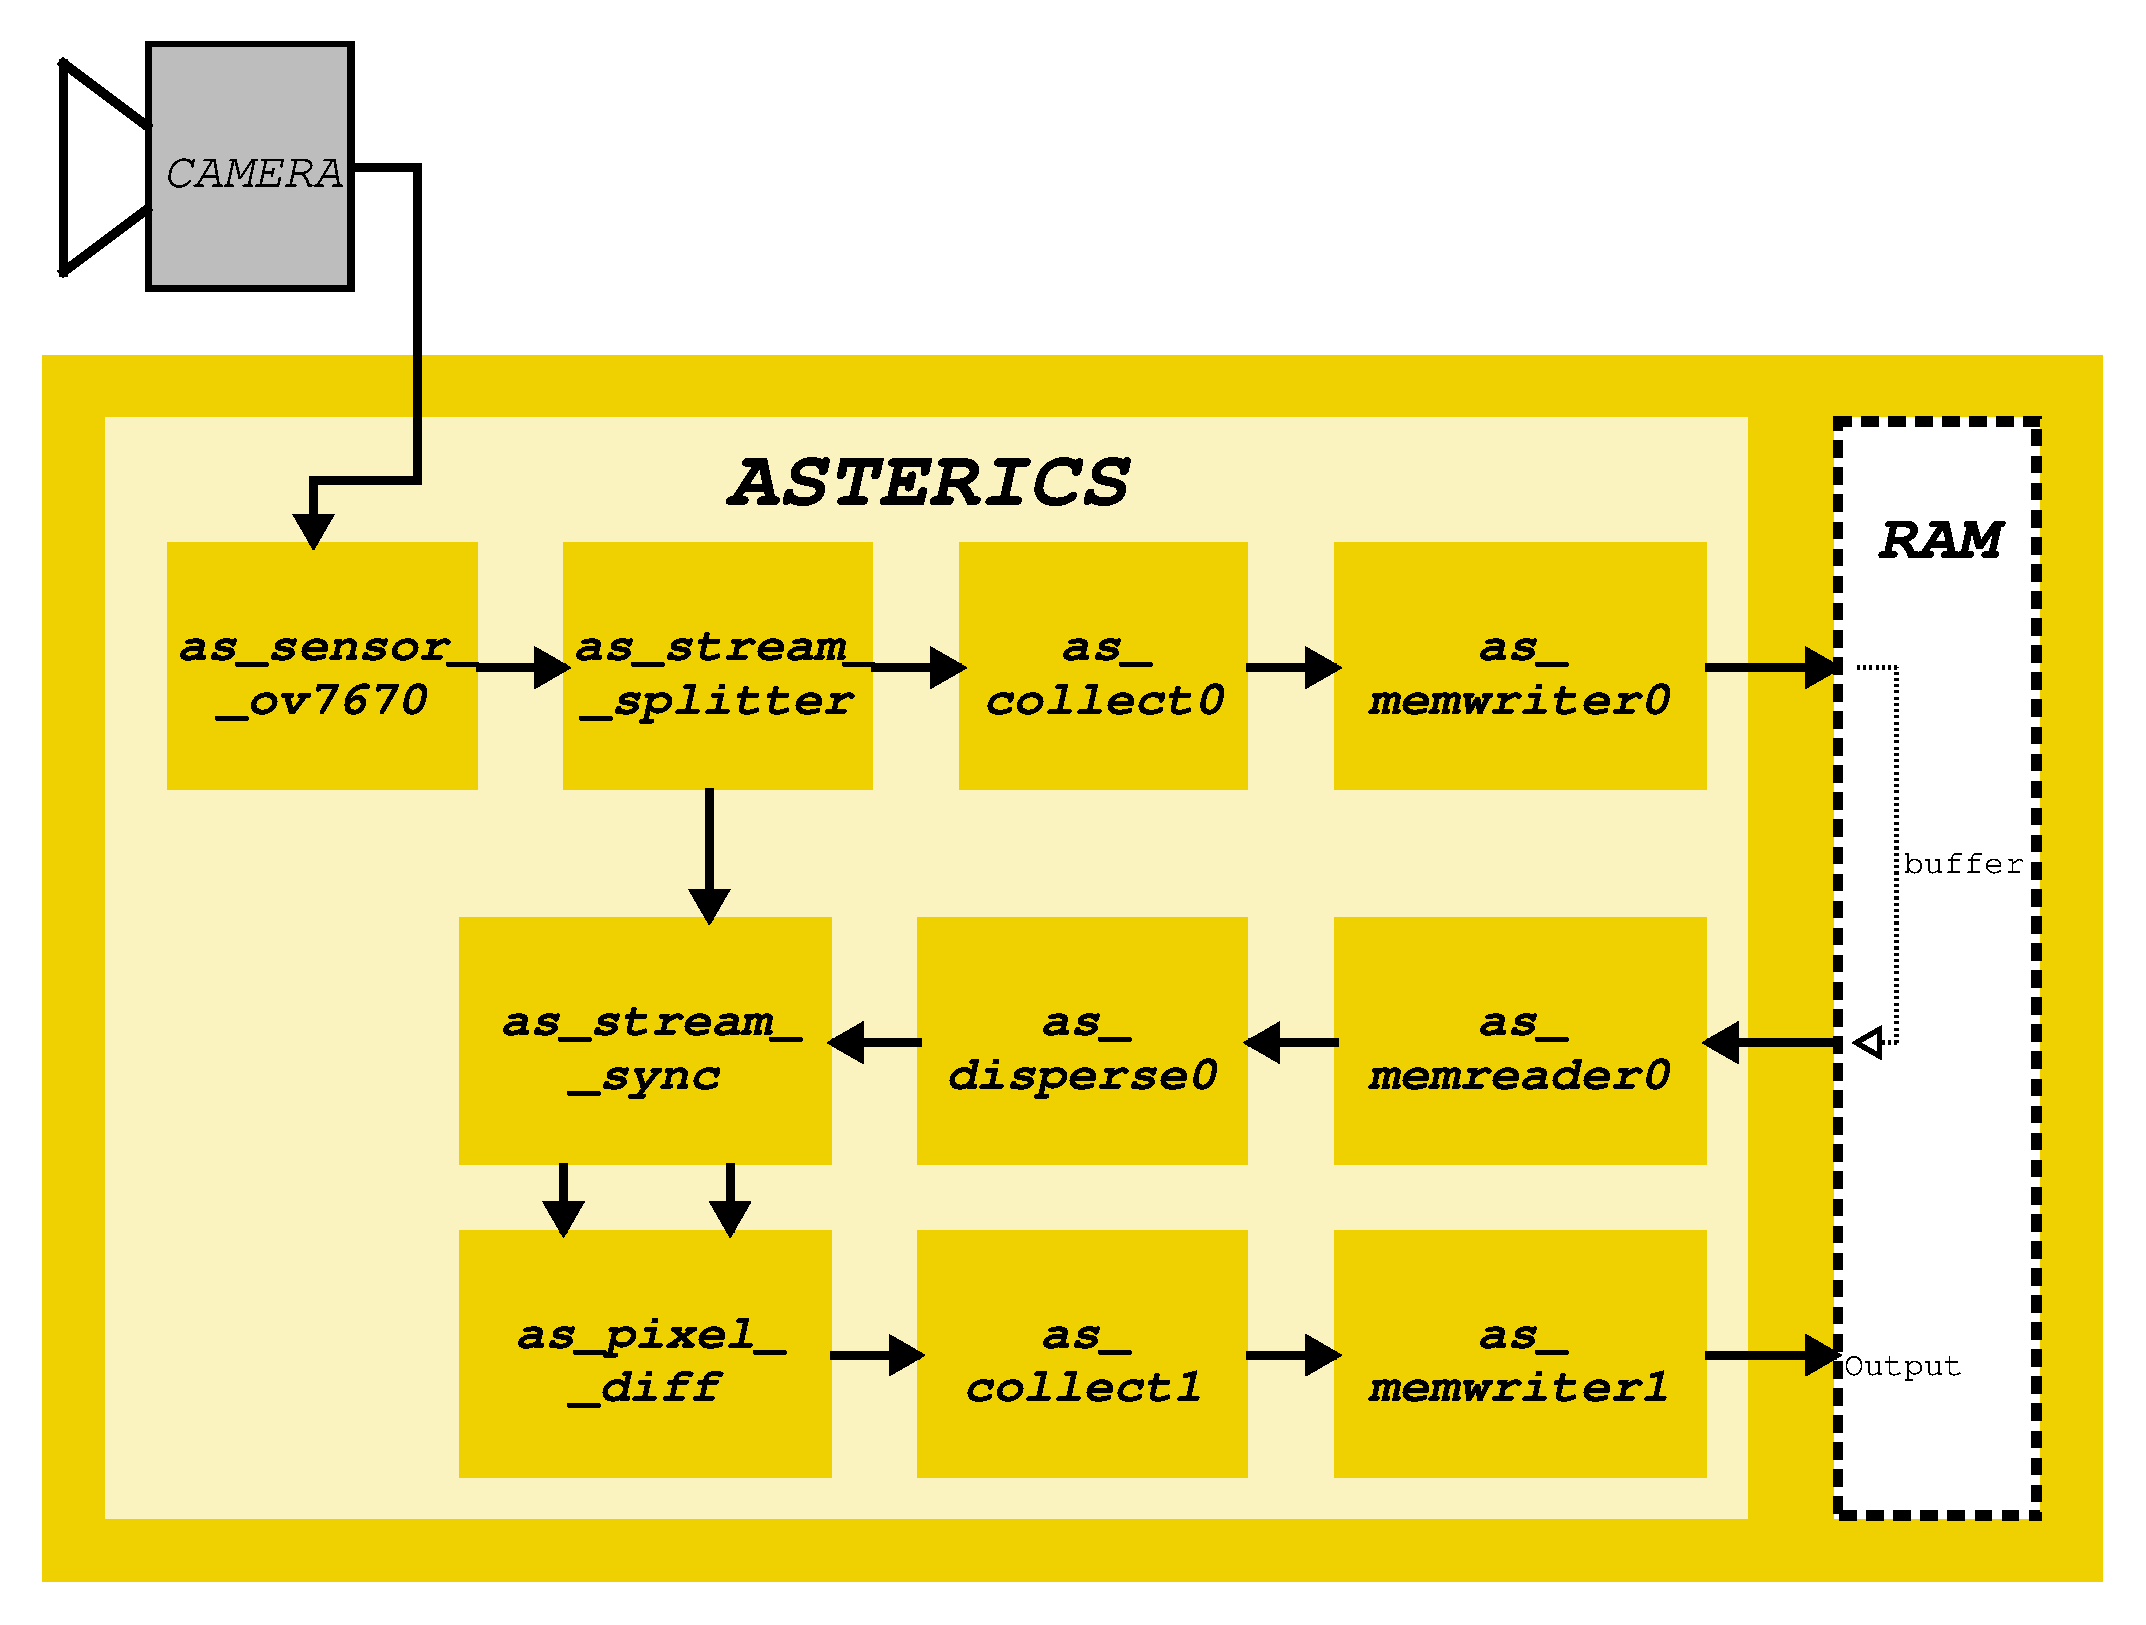
\includegraphics[width=\textwidth]{figs/09-as_refdesign_zybo_image_differencing.pdf}
\caption{Dataflow diagram of the \asterics chain \texttt{as\_refdesign\_zybo}, depicting the included modules.}
\label{fig:09-image_differencing}
\end{figure}

The system architecture is depicted in Figure \ref{fig:09-image_differencing}.
The OV7670 camera is directly connected to the programmable logic and interfaces with an \asterics module \texttt{as\_sensor\_ov7670}.
The physical connection is done via a adapter board or fly-wire connections.
This is detailed in the \texttt{doc} directory of the demo system.
This module converts the camera data stream into a standardized \texttt{as\_stream} interface that the other modules understand.
The data stream is duplicated by the \texttt{as\_stream\_splitter} module.
Each frame is written to RAM by \texttt{as\_memwriter0} from where it is read back when the next frame arrives by the \texttt{as\_memreader0}.
This has the effect of a delay of one frame for this data stream.
The delayed (previous) and duplicated (current) frame are then synchronized by the \texttt{as\_stream\_sync} module and each pixel pair is subtracted from each other by the \texttt{as\_pixel\_diff} module.
The resulting image is then stored in RAM for visualization or further processing.
The \texttt{as\_collect} and \texttt{as\_disperse} modules are used to pack and unpack the eight bit pixel data into 32 bit words for more efficient memory access.
The software for this system is only used to initialize and control the camera and memory access modules and the VEARS core.

This system serves as an example of the capabilities of \asterics and may be used as a starting point and style guide for building your own image processing system using \asterics.
When implemented on the ZyboBoard, switch zero is used to switch between showing the buffered original camera image and the difference image on the screen using the VEARS IP-Core.

For further details regarding building and testing this system, please refer to the included README file and sections \ref{sec:02-getting_started} and \ref{sec:06-02-user_guide}.


\section{as\_refdesign\_canny}
\label{sec:09-01-as_refdesign_canny}
\secauthor{Philip Manke}

\infobox{There are known issues with this system, see section \ref{sec:09-canny_issues}.}

The reference systems \texttt{as\_refdesign\_canny} and \texttt{as\_refdesign\_canny\_dbg} both implement a Canny edge detector using a 2D Window Pipeline subsystem.
Both systems are based on a system developed by Alexander Zoellner and where re-implemented using the 2D Window Pipeline extension of Automatics.
This system is built to demonstrate the 2D Window Pipeline and targets the Zybo-Board development platform.
The system is fully tested for synthesis and implementation using Xilinx Vivado 2019.1.
Note that, just as with the main reference system, \texttt{as\_refdesign\_zybo}, the necessary cable drivers and board files must be installed before building and running the system on hardware.
The system variant \texttt{as\_refdesign\_canny\_dbg} includes additional outputs from the filter modules included in the 2D Window Pipeline, for debugging and educational purposes.

For information on building the system, programming the hardware and operating the software, refer to the README files included in the folders of the systems.

\subsubsection*{System Architecture and Functionality}
\begin{figure}[htbp]
\centering
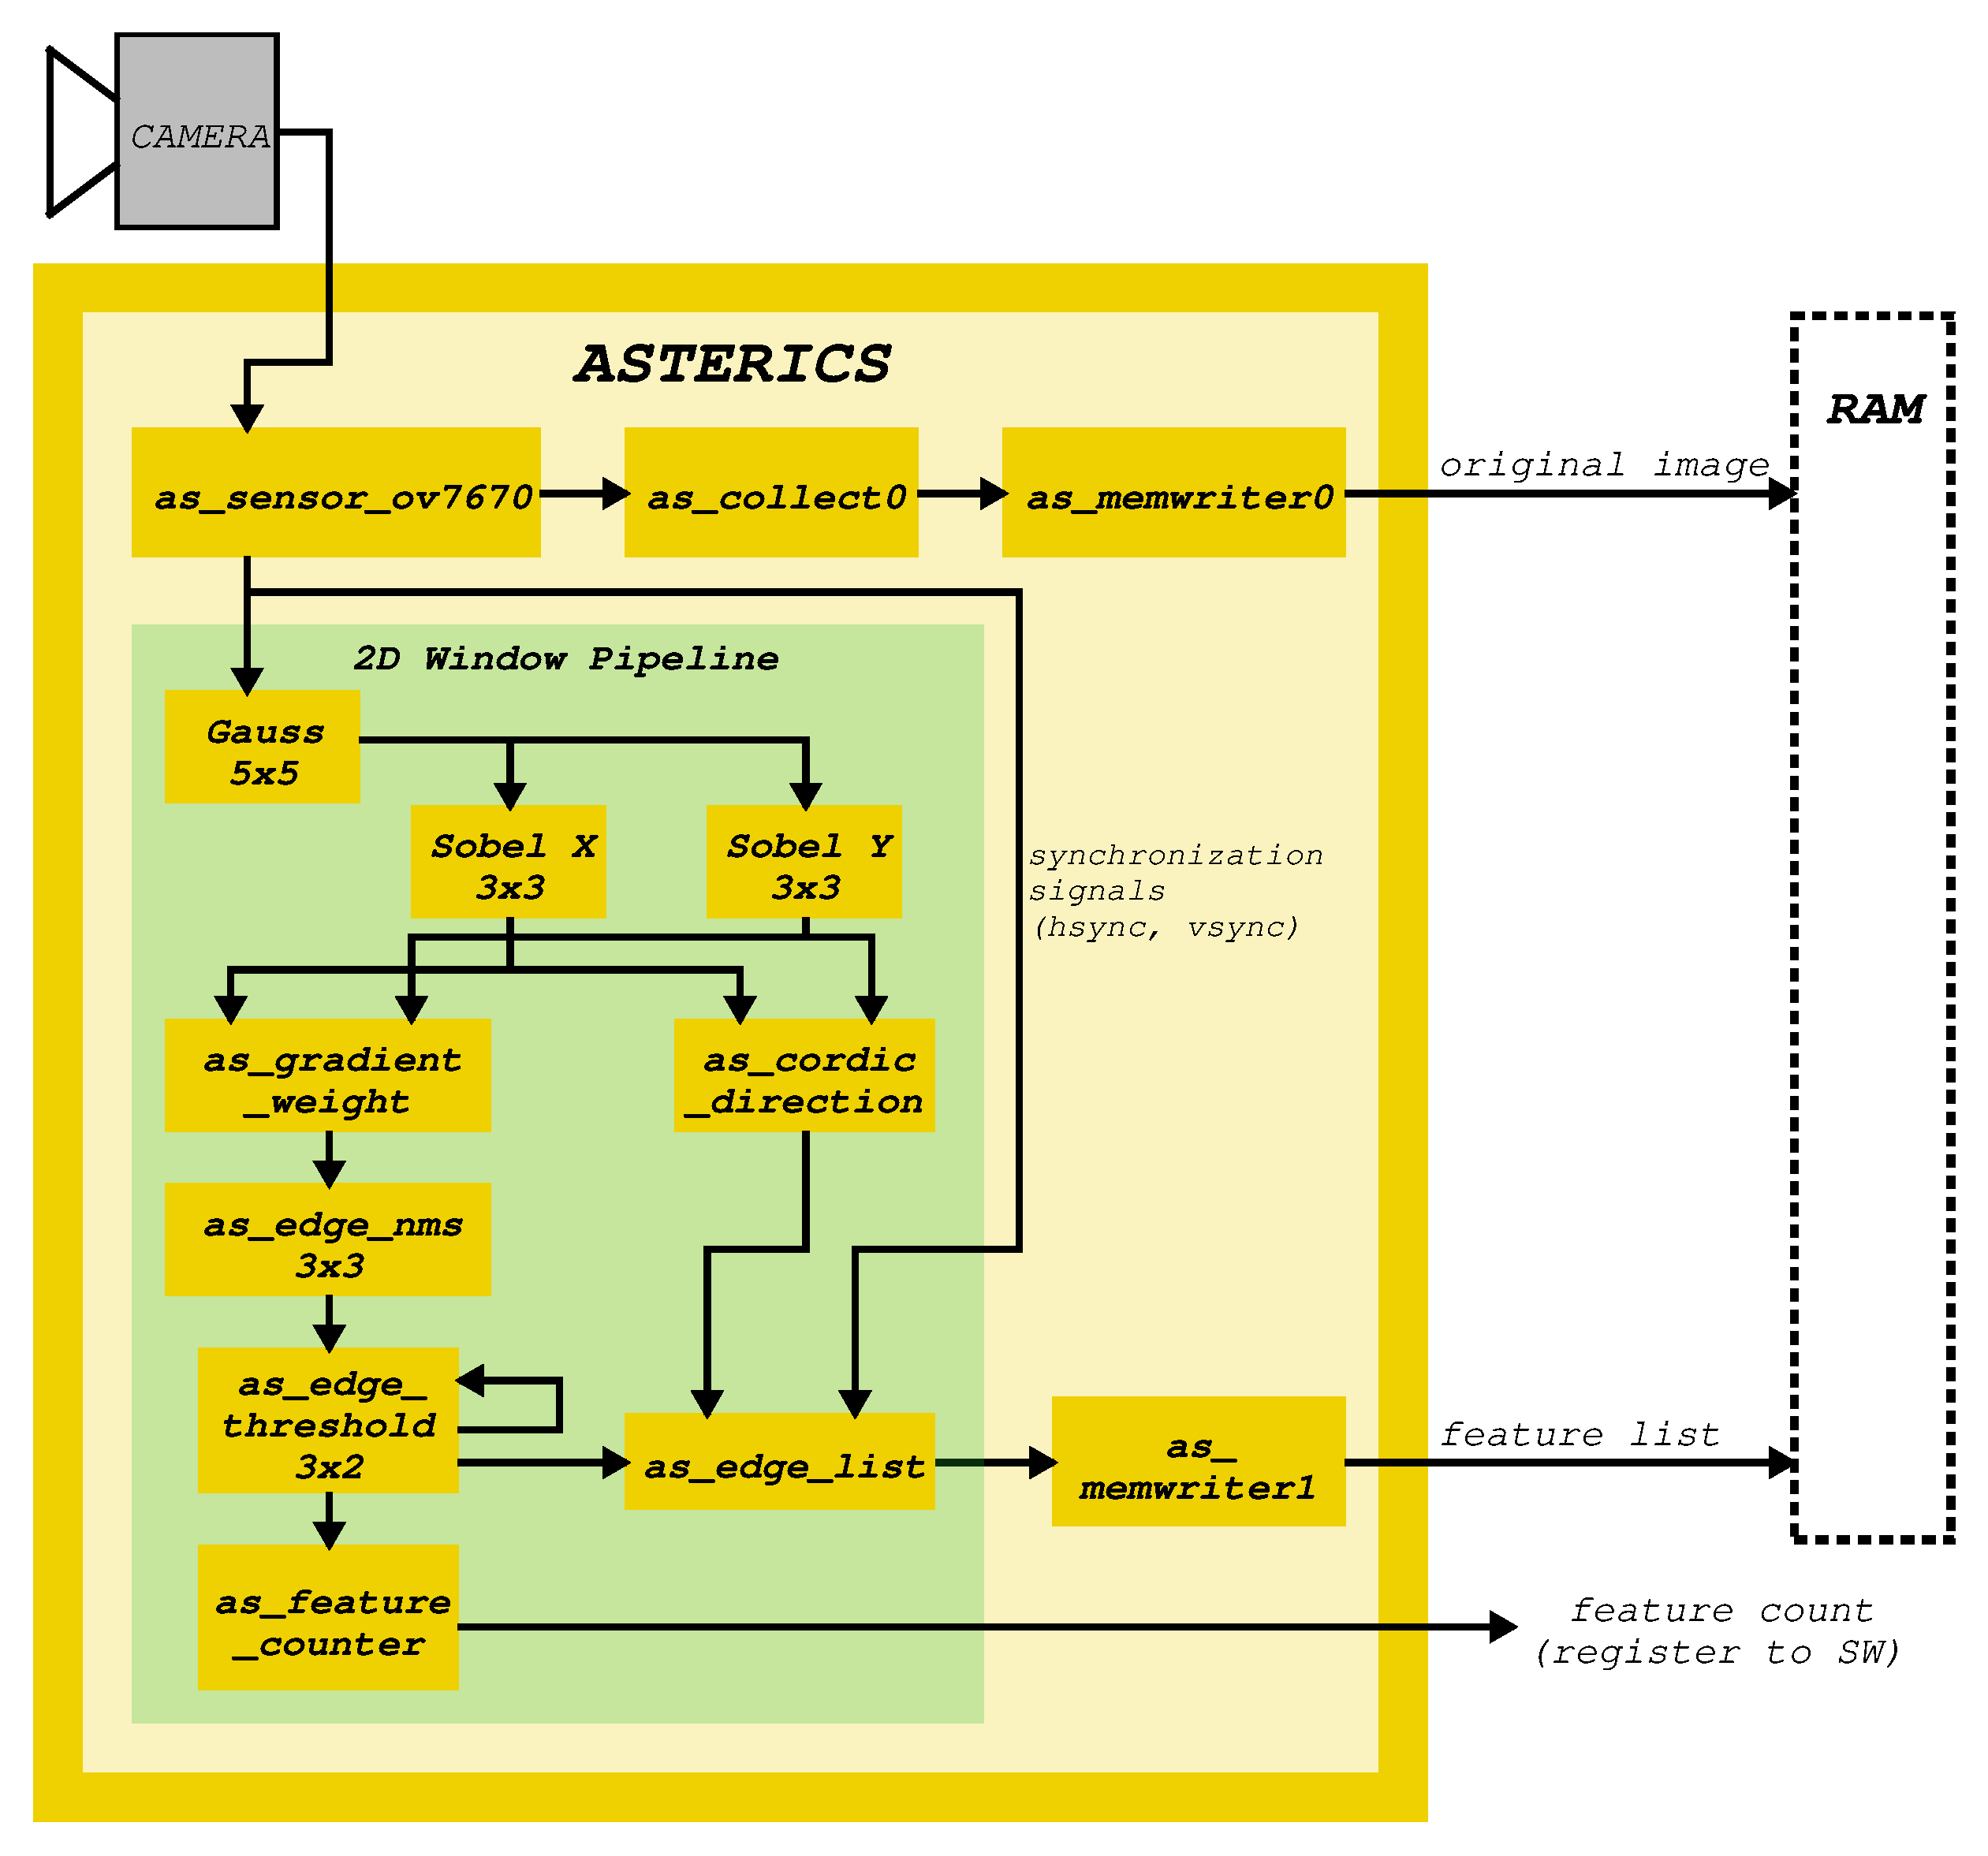
\includegraphics[width=\textwidth]{figs/09-as_refdesign_canny.pdf}
\caption{Dataflow diagram of the \asterics chain \texttt{as\_refdesign\_canny}, depicting the included modules.}
\label{fig:09-canny_diagram}
\end{figure}

The system architecture is depicted in Figure \ref{fig:09-canny_diagram}.
The OV7670 camera is directly connected to the programmable logic and interfaces with the \asterics module \texttt{as\_sensor\_ov7670}.
From there, using the modules \texttt{as\_collect} and \texttt{as\_memwriter}, the original camera image is written to main memory, from where it can be shown on a screen using the VEARS IP-Core, also included with \asterics and in this system.
The Canny edge detector is entirely implemented in a 2D Window Pipeline.
Within the pipeline image convolution with a 5 by 5 Gauss kernel and 3 by 3 Sobel kernels, for both vertical and horizontal edges, is done using three instances of the module \texttt{as\_2d\_conv\_filter\_internal}.
The resulting edge images are combined in the \texttt{as\_gradient\_weight} module and the edge direction is calculated using the Cordic algorithm in the \texttt{as\_cordic\_direction} module.
The combined edge image is filtered for the strongest edge points using a non-maximum-suppression algorithm in the \texttt{as\_edge\_nms} module.
To the now clean edge image, the Canny thresholding is applied in the \texttt{as\_edge\_threshold} module with threshold values provided by software.
The threshold module requires its own output from the last pixel row, requiring a connection to itself.
Lastly this module provides the \texttt{as\_edge\_list} module with the information which pixels are a Canny edge pixel.
The module uses the camera's synchronization signals to generate coordinates for the edge pixels and sends these, together with the Cordic gradient direction to the second \texttt{as\_memwriter} module, writing the Canny features to the main memory.
To inform the software about the number of Canny features written for each camera frame, the \texttt{as\_feature\_counter} module keeps track of the number of Canny edge pixels found and reports that via a slave register.

\section{Known Issues}
\label{sec:09-canny_issues}

This system is not fully tested and debugged.
The following issues unfortunately still exist:

\begin{itemize}
\item The number of reported Canny features per image is not always consistent. In edge cases a very high, incorrect number of features is reported.
\item The memory interface module \texttt{as\_memwriter}, writing the feature data to main memory, sometimes does not finish and reaches a timeout.
\end{itemize}


\section{as\_refdesign\_zynqberry}
\label{sec:09-01-as_refdesign_zynqberry}
\secauthor{Thomas Izycki}

This reference system is designed to serve as a starting point for building processing systems exclusively on the \textit{Zynqberry} using the \asterics framework. The system is tested with Xilinx Vivado 2018.3. Note that just as with all provided reference systems the necessary cable drivers and board files must be installed before building and running the system on hardware.

Beside a \textit{Raspberry Pi} camera v1.3 or 2.1, that has to be connected to the CSI connector, a screen can be attached via HDMI. The system also includes a bare-metal application running on one of the ARM cores, configuring the camera and controlling the ASTERICS chain.

Further information can be obtained by the README files included in the folders of the system.

\subsubsection*{System Architecture and Functionality}

The system architecture is depicted in Figure \ref{fig:09-zynqberry-video-stream}.

\begin{figure}[htbp]
    \centering
    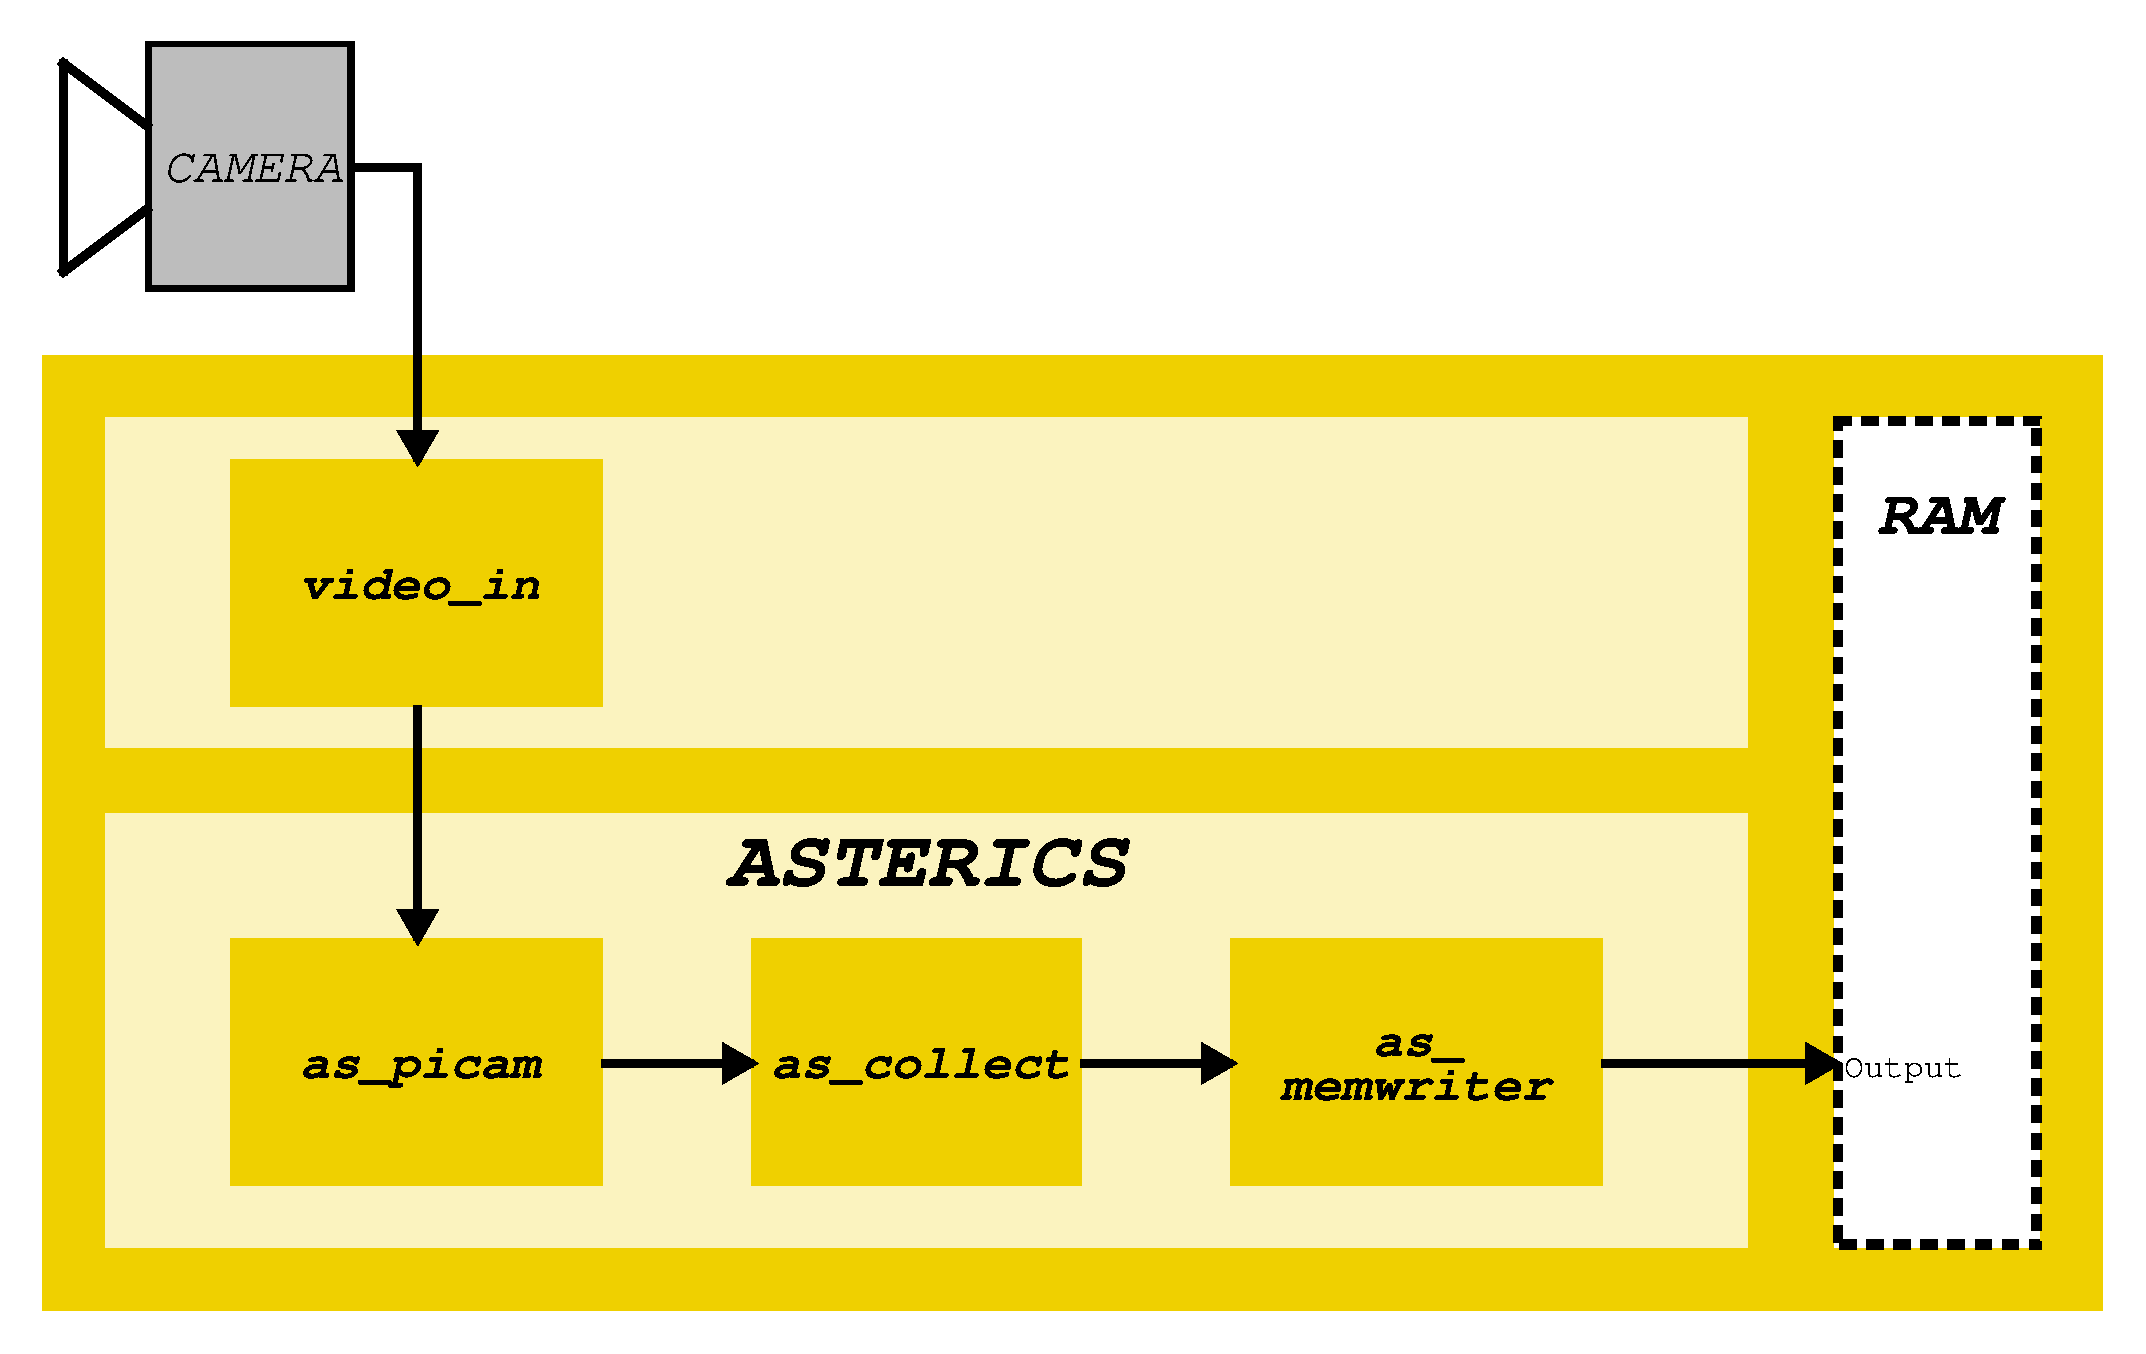
\includegraphics[width=\textwidth]{figs/09-as_refdesign_zynqberry.pdf}
    \caption{Dataflow diagram of the \asterics chain \texttt{as\_refdesign\_zynqberry}, depicting the included modules.}
    \label{fig:09-zynqberry-video-stream}
\end{figure}

 A \textit{Raspberry Pi} camera v1.3 or v2.1 is connected to the \texttt{video\_in} submodule that is not part of the \asterics framework but provided by \textit{Trenz Electronic GmbH} and included in this reference system. The following \texttt{as\_picam} module converts the data stream into a standardized \texttt{as\_stream} interface and computes the grayscale values of the camera images. Subsequent to this module, an own \asterics image processing chain can be built up. In the present case no further image processing takes place and the \texttt{as\_collect} module is used to pack the 8-bit pixel data into 32-bit words for more efficient memory access. The \texttt{as\_memwriter} module writes the images to the main memory. Using the \asterics module for visualization (\textit{VEARS}) IP-Core, the images are shown on the screen attached to the HDMI connector.

 While connected to a computer, the standard output can be displayed on a serial console and might be useful to check the status of the system on start up.

\ifdefined\astericsinternal
\input{09int-systems.tex}
\fi


%%%%%%%%%%%%%%%%%%%%%%%%%%%%% Appendix %%%%%%%%%%%%%%%%%%%%%%%%%%%%%%%%%%

\clearpage

\appendix
\chapter*{Appendices}
\addcontentsline{toc}{chapter}{Appendices}
\renewcommand{\thesection}{\Alph{section}}


\section{Contributing to the \asterics Book}
\secauthor{Philip Manke}

This appendix serves as a guide and reference for contributors to the \asterics book.

\subsection{Who can Contribute?}

All members of the Efficient Embedded Systems (EES) research group working on or with the \asterics framework are urged to write a section or chapter on their work, to help provide a complete documentation of the framework.

All other users of \asterics are also welcome to help complete and improve this document and can do so by sending their suggestions or contributions to one of the main maintainers, as indicated in the preface in \refarb{About this Document}.

\subsection{Language and Style}

This document is written in English.

We strive to keep the content neutral and objective.
Further, we encourage all contributors to base their contributions on scientific publications and professional documentation.

\subsection{\LaTeX{} and Building the \asterics Book}

The \asterics book is written using \LaTeX{} to produce a consistent visual style and reproducible output.
It allows conditionally including parts of the documentation and allows easily collaborating within the EES group.


\subsubsection{Building the \asterics book}


To build the \asterics book, a \LaTeX{} installation must be present on your system.
A Makefile is provided in the directory \texttt{asterics/doc-src/}, capable of producing the PDF output.
All source files for this document are located in \texttt{asterics/doc-src/manual/}.
The produced PDF should be placed in the directory \texttt{asterics/doc/}, so all links are correctly resolved.
\bigskip

\subsubsection{Edititing \LaTeX{}}


For editing and writing \LaTeX{}, any text editor can be used.
We recommend Texmaker\footnote{\url{https://www.xm1math.net/texmaker/}}, as it is rather light-weight, cross-platform, open-source and for its relative simplicity.
\bigskip

\subsubsection{Using \LaTeX{} packages}


\LaTeX{} is a modular typesetting language and supports the use of third-party, often open-source, community developed and maintained packages to extend \LaTeX{} by various features.
The \asterics book includes a number of packages to support the inclusion of different image formats, code with syntax highlighting, local links, URLs and more.
We strongly suggest you make use of the existing packages and only explore the use of other, new packages if no alternative exists.

\warnbox{New \LaTeX{} packages \emph{must not be included} in your contribution without having consulted a maintainer of the \asterics book first.}

Conflicts between \LaTeX{} packages are common and may result in your contribution being unusable without rewriting the parts that require a certain package.
Testing new packages \emph{in the full version of the manual first} is essential.


\subsection{Where Should I Add My Contribution?}

This question should generally be discussed with your supervisor or with one of the maintainers (see preface \refarb{About this Document}).

Generally, it can be helpful to out-source your contribution to a separate file following the existing file naming conventions, especially if your contribution is larger.
The separate file is then included in another file of the document using the \texttt{input} command:
\begin{lstlisting}[style=LaTeXStyle]
§\texttt{\textbackslash}{\texttt{input}}§{my-contribution.tex}
\end{lstlisting}

%input{my-contribution.tex}
%\end{lstlisting}


\subsection{Conventions and Brief Reference Guide}

Within the \asterics book we observe a set of conventions regarding the formatting of text, font styles, listings, tables, references and more.
This section gives an overview over these and may serve as a reference when contributing to this document.
It is not exhaustive and only presents a subset of the most commonly used \LaTeX{} commands.

\subsubsection{General Conventions}
~~
\textbf{Attribution:}
\smallskip

Chapters, sections or (sub-)subsections that are entirely or almost entirely written by a single author or very few authors, should be marked as such.
This document includes two commands to easily add this information:
\begin{itemize}
\item For any part authored by one or two (maybe three) authors, use the following below your chapter, section or (sub-)subsection:
\begin{lstlisting}[style=LaTeXStyle]
\secauthor{<authorname>[, <second author>]}
\end{lstlisting}
If more than two (three) authors have worked on a chapter, section, etc, this should not be used and instead be left unmarked.

\item For any chapter, section, etc, formerly authored by a single author and edited by you substantially, change the above command to:
\begin{lstlisting}[style=LaTeXStyle]
\secorigauthor{<authorname>[, <second author>]}
\end{lstlisting}
\end{itemize}

\textbf{Referring to \asterics:}
\smallskip

To reference the \asterics project, a \LaTeX{} command exists that consistently reproduces the style chosen to represent the \asterics framework in this document.
Any time you refer to the framework by name, the following command must be used:

\begin{lstlisting}[style=LaTeXStyle]
\asterics
\end{lstlisting}

\subsubsection{Font Styles}

Within this document the following three font styles are used to accentuate the following:
\begin{itemize}
\item \textbf{Bold style font} is used to define names and terms you deem important and/or that are used often within the document / chapter / section.
\begin{lstlisting}[style=LaTeXStyle]
\textbf{text you want to print in bold}
\end{lstlisting}

\item \textit{Italic style font} is used to highlight important text, phrases or words you want the reader to pay special attention to.
\begin{lstlisting}[style=LaTeXStyle]
\emph{text you want to print in italic}
 - or - 
\textit{text you want to print in italic}
\end{lstlisting}

\item \texttt{Typewriter style font} is used to highlight directories, file paths, file names and function, parameter, class names or similar things.
Anything more than singular names, concerning code inclusions in written text, should be done using the \texttt{lstlisting} environment, explained in Section \refarb{Code Listings} of this appendix.
\begin{lstlisting}[style=LaTeXStyle]
\texttt{text you want to print in typewriter}
\end{lstlisting}
\end{itemize}

\subsubsection{Chapters, Sections and Subsections}

This document is organized using the following levels in descending hierarchy: chapters, sections, subsections and subsubsections.
If you believe that another level below the subsubsection would be helpful/required, consider restructuring your text.
Only if this is not possible, use:
\begin{lstlisting}[style=LaTeXStyle]
§{\texttt{\textbackslash}}subsubsection*§{Name of the Subsubsection}
\end{lstlisting}
This will create a non-numbered heading of the same fontsize and style as a subsubsection.

\warnbox{Starred sections will not appear in the table of context, thus will be harder to find!}

Typically, each chapter and section is labeled, to more easily reference it throughout the document. See Section \refarb{Referencing} for more information.

\subsubsection{Referencing}
\labelarb{Referencing}

In general, to reference something in \LaTeX{}, a label has to be first set.
Chapters, (sub-) sections, figures, tables, code listings and more can be labeled and referenced throughout the document.
References create clickable links that link to the location in the document of the referenced label.

This document includes helpful commands for referencing different targets:

\begin{itemize}
\item \textbf{Chapters:}
\begin{lstlisting}[style=LaTeXStyle]
§{\textbackslash}\texttt{chapter}§{Example Chapter}
\labelch{<internal label name>}
% [...]
Xyz is described in \refch{<internal label name>}.
% This prints as: "§{\textrm{Xyz is described in Chapter 2.}§"
\end{lstlisting}

\item \textbf{Sections:}
\begin{lstlisting}[style=LaTeXStyle]
§{\textbackslash}\texttt{section}§{Example Section}
\labelsec{<internal label name>}
% [...]
Xyz is described in \refsec{<internal label name>}.
% This prints as: "§{\textrm{Xyz is described in Section 2.3.}§"
\end{lstlisting}

\item \textbf{(Sub-)Subsections:}
\begin{lstlisting}[style=LaTeXStyle]
§{\textbackslash}\texttt{subsection}§{Example Subsection}
\labelssec{<internal label name>}
% [...]
Xyz is described in \refssec{<internal label name>}.
% This prints as: "§{\textrm{Xyz is described in Section 2.3.1.}§"
\end{lstlisting}

\item \textbf{Figures:}
\begin{lstlisting}[style=LaTeXStyle]
§{\textbackslash}§begin{figure}
% [...]
\labelfig{<internal label name>}
§{\textbackslash}§end{figure}
% [...]
Xyz is shown in \reffig{<internal label name>}.
% This prints as: "§{\textrm{Xyz is shown in Figure 2.1.}§"
\end{lstlisting}

\item \textbf{Tables:}
\begin{lstlisting}[style=LaTeXStyle]
§{\textbackslash}§begin{table}
% [...] Table
\labeltab{<internal label name>}
§{\textbackslash}§end{table}
% [...]
Xyz is provided in \reftab{<internal label name>}.
% This prints as: "§{\textrm{Xyz is provided in Table 2.1.}§"
\end{lstlisting}

\item \textbf{Hardware Modules:}
\begin{lstlisting}[style=LaTeXStyle]
\labelmodule{<module name>}
% [...]
, in this case, consider using \refmodule{<module name>}.
% This prints as: "§{\textrm{, in this case, consider using }\texttt{<module name>}}§"
\end{lstlisting}

\item \textbf{Tools:}
\begin{lstlisting}[style=LaTeXStyle]
\labeltool{<tool name>}
% [...]
The tool \refmodule{<module name>} simplifies this operation.
% This prints as: "§{\textrm{The tool }\texttt{<tool name>}\textrm{ simplifies this operation.}}§"
\end{lstlisting}

\item \textbf{Arbitrary Locations by Name:}
\begin{lstlisting}[style=LaTeXStyle]
\labelarb{<name>}
% [...]
See Section \refarb{<name>} in the preamble.
% This prints as: "§{\textrm{See Section \texttt{<}\textit{name}\texttt{>} in the preamble.}}§"
\end{lstlisting}

\end{itemize}

\textbf{Code listings} must be labeled and referenced manually, using the built-in \LaTeX{} label and reference commands:
\begin{lstlisting}[style=LaTeXStyle]
§\textbackslash§begin{lstlisting}[style=[...], label=lst:<label name>]
% [...]
§\textbackslash§end{lstlisting}
% [...]
Listing \ref{lst:<label name>} shows a relevant code example.
% This prints as: "§{\textrm{Listing 3.1 shows a relevant code example.}}§"
\end{lstlisting}

To refer to the Doxygen documentations of the different parts of the framework, the following commands are available:

\begin{itemize}
\item \textbf{Python code:} \lstinline[style=LaTeXStyle]{\refdoxypython}, prints as: \refdoxypython


\item \textbf{C code:} \lstinline[style=LaTeXStyle]{\refdoxyc}, prints as: \refdoxyc

\item \textbf{VHDL code:} \lstinline[style=LaTeXStyle]{\refdoxyvhdl}, prints as: \refdoxyvhdl

\end{itemize}


\subsubsection{Info and Warning Boxes}

To especially highlight some information, this document includes two types of information "boxes".

\begin{itemize}

\item \textbf{Information Box:}
\begin{lstlisting}[style=LaTeXStyle]
\infobox{Hello, I am a friendly looking information box.}
\end{lstlisting}
This prints as:
\infobox{Hello, I am a friendly looking information box.}

\item \textbf{Warning Box:}
\begin{lstlisting}[style=LaTeXStyle]
\warnbox{Please pay attention, I am a warning box!}
\end{lstlisting}
This prints as:
\warnbox{Please pay attention, I am a warning box!}

\end{itemize}

\subsubsection{Including Images/Figures}

Images or figures are very helpful to illustrate more complex concepts or to provide examples and overviews of topics.
We encourage the use of figures, but be aware of the following:
\begin{itemize}
\item 
Make sure that you are legally allowed to use an image when it comes from a third party.
Check that it can be distributed under the Creative Commons Attribution-ShareAlike 4.0 International License, which this document is published under.
Be sure you fulfill all obligations of the license that an image is published under, when you include third party content.

Or alternatively, create the image/figure yourself, but be aware that it will be published under the CC-SA 4.0.

\item
Use high quality images and figures, ideally vector graphics (e.g. SVG) for figures and good quality JPEGs, PNGs or similar for photos.
Be aware of the file sizes.
Ideally you should strike a balance between sharp images/figures and acceptable file sizes.

\item
Vector graphics must be packed into PDF files to be used in this document.
We suggest you use Inkscape\footnote{\url{https://inkscape.org/}} to easily convert vector graphic files to PDF files.
\end{itemize}

To include a figure use the following syntax:
\begin{lstlisting}[style=LaTeXStyle]
\begin{figure}[htbp]
§{\texttt{\textbackslash}}§centering  % optional
\includegraphics[width=0.8\textwidth]{path/to/file.png}
\caption{Brief description of this figure}
\label{fig:<labelname>}
§{\texttt{\textbackslash}}§end{figure}
\end{lstlisting}

The tag \texttt{[htbp]} in the first line describes roughly, where \LaTeX{} should place the figure and with what priority.
The letters mean the following: \texttt{h}: here, \texttt{t}: top of a page, \texttt{b}: bottom of a page, \texttt{p}: on its own page.
You may omit any (or all) and rearrange them to fit your needs.

The \texttt{{\textbackslash}centering} command centers the figure horizontally on the page.

The decimal number within the statement "\texttt{width=0.8{\textbackslash}textwidth}", in this example \texttt{0.8}, defines the percentage ($0.8 = 80\%$) of the page the figure should occupy.
Only the portion of the page, where text is printed, is considered.

\subsubsection{Lists and Enumerations}

\LaTeX{} supports two types of listings:

\begin{itemize}
\item \textbf{itemize:} Itemize listings are unnumbered, bullet point lists, like this one. Create them using:
\begin{lstlisting}[style=LaTeXStyle]
§\textbackslash§begin{itemize}
§\textbackslash§item <First point here
  Still part of the first point.>
§\textbackslash§item <Second point here>
§\textbackslash§end{itemize}
\end{lstlisting}

\item \textbf{enumerate:} Enumerate listings are numbered lists. Create them using:
\begin{lstlisting}[style=LaTeXStyle]
§\textbackslash§begin{enumerate}
§\textbackslash§item <First point here
  Still part of the first point.>
§\textbackslash§item <Second point here>
§\textbackslash§end{enumerate}
\end{lstlisting}

\end{itemize}

\subsubsection{Tables}

To present data in a table environment, two templates are provided here:

\begin{itemize}
\item \textbf{Smaller tables:}
\begin{lstlisting}[style=LaTeXStyle]
\begin{table}[htbp]
§{\texttt{\textbackslash}}§centering  % optional
\begin{tabular}{|l|c|r|}
  \hline  % Column headers
  \textbf{Header 1} & \textbf{Header 2} & \textbf{Header 3} \\
  \hline  % First data row
  Data 1 & Data 2 & Data 3 \\
  \hline  % Second data row
  Data 1 & Data 2 & Data 3 \\
  \hline
§{\texttt{\textbackslash}}§end{tabular}
\caption{<Short description of the table>}
\labeltab{<label name>}
§{\texttt{\textbackslash}}§end{table}
\end{lstlisting}
This prints as:
\begin{table}[htbp]
\centering  % optional
\begin{tabular}{|l|c|r|}
  \hline  % Column headers
  \textbf{Header 1} & \textbf{Header 2} & \textbf{Header 3} \\
  \hline  % First data row
  Data 1 & Data 2 & Data 3 \\
  \hline  % Second data row
  Data 1 & Data 2 & Data 3 \\
  \hline
\end{tabular}
\caption{Short description of the table}
\end{table}

To adjust the number of columns and the alignment of text within table cells, adjust the column definition characters within the \texttt{tabular} environment:
\begin{lstlisting}[style=LaTeXStyle]
\begin{tabular}{|l|c|r|}
\end{lstlisting}
Where \texttt{l} defines a left aligned column, \texttt{c} defines a centered column and \texttt{r} defines a right aligned column.

For especially small tables the \texttt{table} environment can be removed, using only \texttt{tabular}.

\item \textbf{Larger tables with multi-line cells:}
\begin{lstlisting}[style=LaTeXStyle]
\begin{longtable}[htbp]{|c|c|c|}
\hline  % Column headers
\textbf{Header 1} & \textbf{Header 2} & \textbf{Header 3} \\
\hline  % First data row
\endhead  
\texttt{Data 1} & Data 2 &
\parbox{11cm}{\ \\ Multi-line description text or other long data, maybe a list?
Who knows, it's your documentation, not mine. 
\vspace{0.3em}} \\
\hline  % Second data row
\texttt{Data 1} & Data 2 &
\parbox{11cm}{\ \\ Multi-line description text.
\vspace{0.3em}} \\
\hline
\caption{Brief description of the table}
\labeltab{<label name>}
§{\texttt{\textbackslash}}§end{longtable}
\end{lstlisting}
This prints as:
\begin{longtable}[htbp]{|c|c|c|}
\hline  % Column headers
\textbf{Header 1} & \textbf{Header 2} & \textbf{Header 3} \\
\hline  % First data row
\endhead  
\texttt{Data 1} & Data 2 &
\parbox{11cm}{\ \\ Multi-line description text or other long data, maybe a list? Who knows, it's your documentation, not mine.
\vspace{0.3em}} \\
\hline  % Second data row
\texttt{Data 1} & Data 2 &
\parbox{11cm}{\ \\ Multi-line description text.
\vspace{0.3em}} \\
\hline
\caption{Brief description of the table}
\labeltab{<label name>}
\end{longtable}

The width of the multi-line text cells, using the \texttt{parbox} command, can be easily adjusted using the first parameter:
\begin{lstlisting}[style=LaTeXStyle]
\parbox{<width>cm}{ Text }
\end{lstlisting}

\end{itemize}

\subsubsection{Code Listings}
\labelarb{Code Listings}

Code listings should be placed within the \texttt{lstlisting} environment.
Use the following syntax:
\begin{lstlisting}[style=LaTeXStyle]
§\textbackslash§begin{lstlisting}[style=<listing style>,
	label=lst:<labelname>, caption=<Brief description of the code>]
Add your code here
§\textbackslash§end{lstlisting}
\end{lstlisting}

The following styles are available within the \asterics book:
\begin{itemize}
\setlength{\itemsep}{-0.3em}
\item \texttt{CStyle} for C code
\item \texttt{hdl} for VHDL code
\item \texttt{LaTeXStyle} for \LaTeX{} code
\item \texttt{AutomaticsPython} for Python code (specifically Automatics Scripts)
\end{itemize}
Additional styles should be added to the file \texttt{asterics/doc-src/00-lst-settings.tex}.

For especially short code examples or if you want to use syntax highlighting on single words, like function or class names or keywords, consider using the inline syntax:

\begin{lstlisting}[style=LaTeXStyle]
§\textbackslash§lstinline[style=<listing style>]{Your code here}
\end{lstlisting}

Three convenience commands are currently available in this document:
\begin{itemize}
\setlength{\itemsep}{-0.2em}
\item \texttt{{\textbackslash}lstapyinline\{Your code here\}} for Python code
\item \texttt{{\textbackslash}lsthdlinline\{Your code here\}} for VHDL code
\item \texttt{{\textbackslash}lstcinline\{Your code here\}} for C code
\end{itemize}

\subsubsection{URLs and Linking to Files}

\LaTeX{} supports linking to URLs and local files.

\begin{itemize}
\item \textbf{Third party websites:} When linking to third party websites, we suggest you use a footnote and print the URL in full, so readers can clearly see where the link will take them. Were fitting, URLs may also be placed within the text. Note that text wrapping issues may arise for long URLs.
\begin{lstlisting}[style=LaTeXStyle]
We suggest the use of \LaTeX{}§\textbackslash§footnote{§\textbackslash§url{https://www.latex-project.org/}}.
\end{lstlisting}
This prints as:\\
We suggest the use of \LaTeX{}\footnote{\url{https://www.latex-project.org/}}.

\item \textbf{Known, internal websites:} Websites, such as the homepage of the EES-group, may be included as follows:
\begin{lstlisting}[style=LaTeXStyle]
For more information, see the \href{https://ees.hs-augsburg.de}{EES Homepage}.
\end{lstlisting}
This prints as:\\
For more information, see the \href{https://ees.hs-augsburg.de}{EES Homepage}.

\item \textbf{Files:} Linking to files should be done using their relative position in the file system - relative to the position of this manual.
The PDF file \textbf{must} be placed in \texttt{asterics/doc/} for these links to function.
All file links \textbf{must} use this folder as the root for relative file links.
\begin{lstlisting}[style=LaTeXStyle]
The \href{run:./VHDL_doxygen/html/index.html}{Doxygen documentation}
provides more detail.
\end{lstlisting}
This prints as:\\
The \href{run:./VHDL_doxygen/html/index.html}{Doxygen documentation}
provides more detail.

\end{itemize}



\clearpage

\section{Doxygen Cheatsheet}
\secauthor{Philip Manke}

Besides the documentation written for the \asterics book specifically, the framework is also documented per programming language using the Doxygen tool.
This section serves as a reference for general and language specific functions and rules for writing code that produces Doxygen documentation of high quality.

Doxygen is a tool to automatically parse source code and generate documentation from the code and comments.
Doxygen does not parse all comments, only those started using specific characters, dependent on the programming language.

Within Doxygen comments, simple Markdown syntax, such as \texttt{**bold**} and \texttt{//italic//} can be used to format text.
Using the name of other documented code entities, such as classes and functions, will automatically highlight them and add a link to their documentation.


\subsection{Doxygen Comments}

\subsubsection{C Code}

Valid Doxygen comments include:

\begin{lstlisting}[style=CStyle]
/// Doxygen comment

//! Doxygen comment

/**
 * Multi-line Doxygen comment
 */
\end{lstlisting}

\subsubsection{VHDL Code}

Doxygen comments are started using:
\begin{lstlisting}[style=hdl]
--! Doxygen comment
\end{lstlisting}

\subsubsection{Python Code}

In Python, single and multi-line Doxygen comments are started as follows:
\begin{lstlisting}[style=AutomaticsPython]
## Doxygen comment
#  All comments until an empty line are also Doxygen comments

# Regular comment
\end{lstlisting}

Furthermore, docstrings can also be parsed by Doxygen:
\begin{lstlisting}[style=AutomaticsPython]
def example_function():
    """I am a regular docstring. I describe "example_function"."""

def doxygen_example_function():
    """! @brief I am a Doxygen-parsed docstring.
    The exclamation mark makes Doxygen parse me.
    I describe "doxygen_example_function"."""
\end{lstlisting}

\clearpage

\subsection{General Commands and Tags}

Each Doxygen command and tag must be preceded by either a backslash (\texttt{\textbackslash}) or an "at"-character (\texttt{@}) to distinguish it from a regular word.

\begin{itemize}
\item \texttt{@author}: This tag allows to define an author for a file, class, function, etc.
\begin{lstlisting}[style=CStyle]
/// @file filename.c
/// @author <author name>
\end{lstlisting}

\item \texttt{@file}: This command allows to add a description to the file.
\begin{lstlisting}[style=CStyle]
/// @file filename.h
/// <description>
\end{lstlisting}

\item \texttt{@brief}: Define part of a Doxygen comment as a short summary. This is displayed more prominently in the resulting documentation and should always be included.
\begin{lstlisting}[style=CStyle]
/// @brief This is a summary for as_iic_init, it ends at the 
/// first sentence/full stop, right here ->.
/// <detailed description from here on>
void example_function(){ // [...] 
\end{lstlisting}

\item \texttt{@param}: This tag defines the description of a function parameter.
\begin{lstlisting}[style=CStyle]
/// @param value1  <Description of the parameter value1>
/// @param value2  <Description of the parameter value2.
///                 Can span multiple lines and sentences.>
void example_function(int value1, int value2){ // [...]
\end{lstlisting}

\item \texttt{@return}: This tag defines the description of a function's return value.
\begin{lstlisting}[style=CStyle]
/// @return  <Description of the return value>
int example_function(){ // [...]
\end{lstlisting}

\item \texttt{@defgroup}: Creates a group/module for within the documentation. Allows thematic/functional grouping of code documentation.
\begin{lstlisting}[style=CStyle]
/// @defgroup <internal group name> <group display name> 
/// @brief <Summary of group description>
/// <Detailed descripton from here on>
\end{lstlisting}

\item \texttt{@\{} and \texttt{@\}}: These braces can be used in conjunction with some Doxygen commands to define their scope. For example with \texttt{@addtogroup}.

\item \texttt{@addtogroup}: Add a scope to a Doxygen group/module.
\begin{lstlisting}[style=CStyle]
/// @addtogroup <internal group name>
/// @{
  
// Things to add to the group

/// @}
\end{lstlisting}

\item \texttt{@ingroup}: Add a single file, class, function, etc. to a group.
\begin{lstlisting}[style=CStyle]
/// @ingroup <internal group name>
void example_function(){ // [...]
\end{lstlisting}

\end{itemize}




% TBD(AZ,CS,DM,MS):   [GK 2018-07-09]
%   Wir sollten noch ein Kapitel "Systems hinzufügen" (s.o.), um auch komplette
%   Systeme zu beschreiben. Aktuell:
%   a) Das Demo-System / evtl. separat das EdS-2-System
%   b) Das System aus dem ASAP-Paper
%   c) Das System aus dem FSD-Fahrzeug
%
%   Nicht-öffentliche Systeme und Module sollten in Unterdateien mit den Namen
%
%     07int-mod-<Modulname>.tex     (Module)
%     08int-sys-<Systemname>.tex    (Systeme)

%   dokumentiert werden. Für freie Systeme und komplexe Module sollte wir die gleiche
%   Namenskonvention ohne "int" einführen.
%





%%%%%%%%%%%%%%%%%%%%%%%%%%%%% Bibliography %%%%%%%%%%%%%%%%%%%%%%%%%%%%%%%%%%%



%\printbibliography[heading=bibintoc]

\end{document}
